\chapter{Graphs}
\label{sec:graphs}

\section{Simulated FWI variables}
Este local não teve incêndio
\begin{figure}[h]
\caption{HELLo}
    \centering
    \begin{subfigure}{0.49\textwidth}
        \centering
        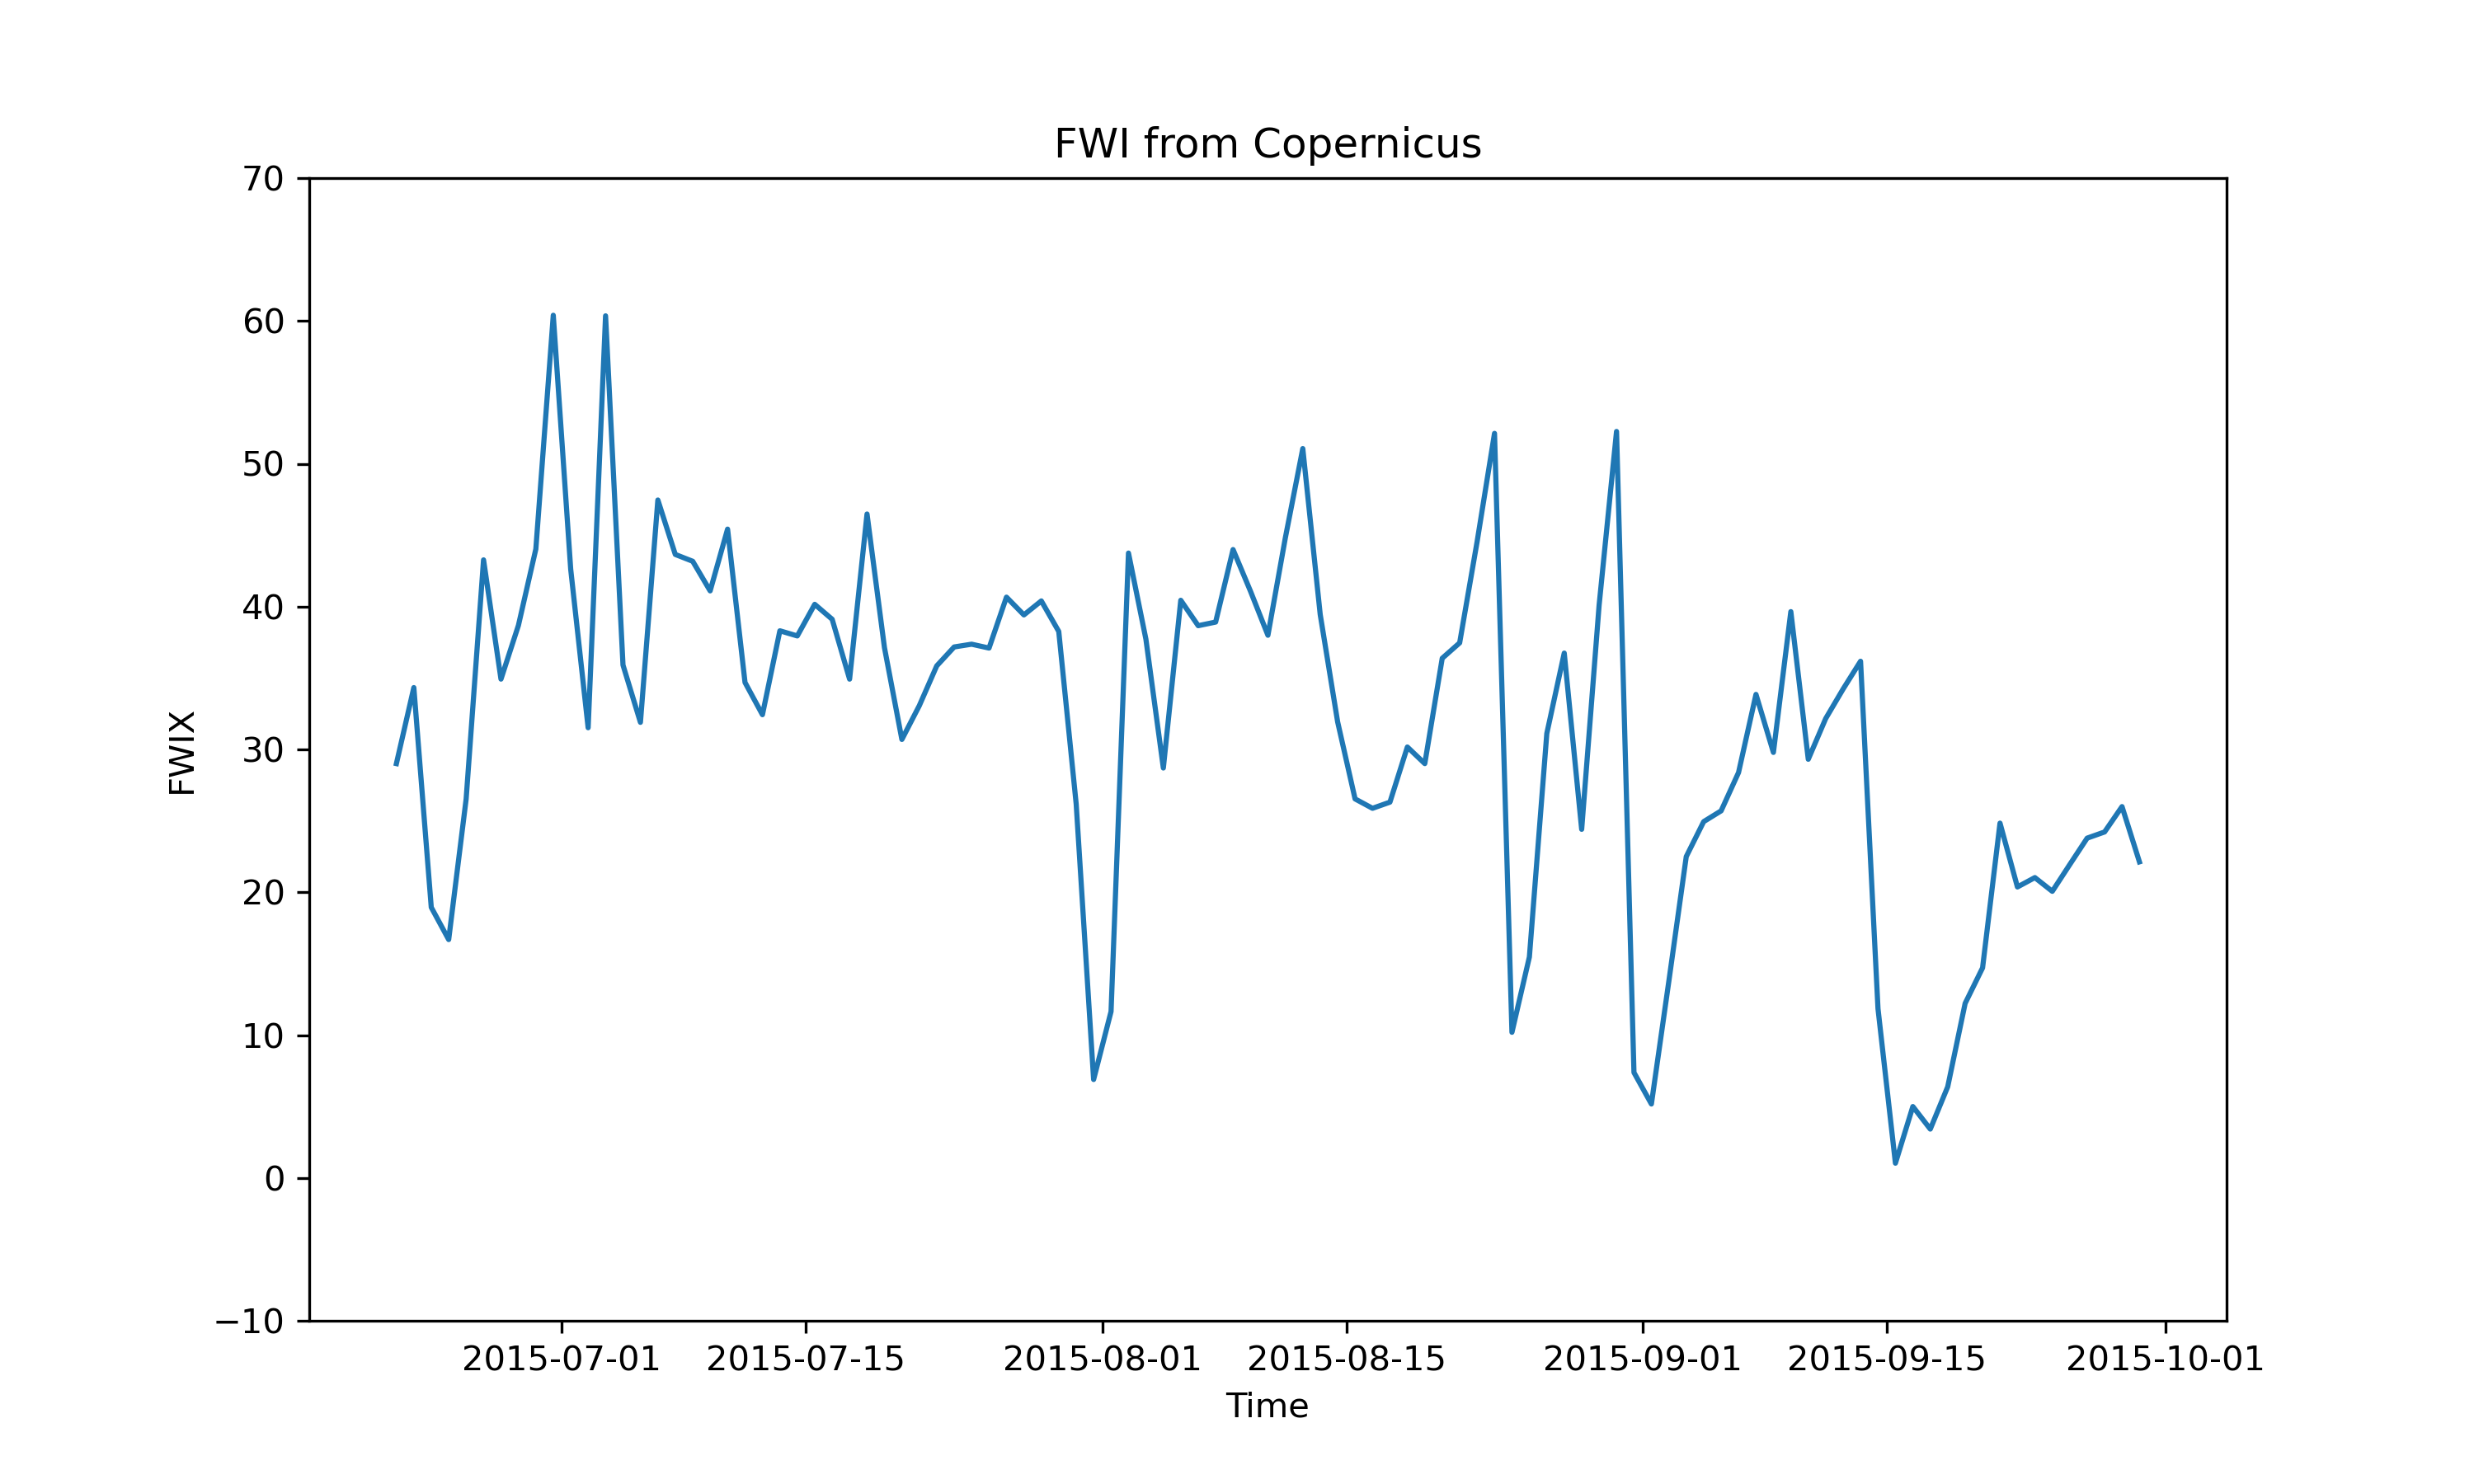
\includegraphics[width=\textwidth]{graphs/2015MesmoSitio/2015CopernicusFWI12.png}
        \caption{Caption for image 1}
        \label{fig:img1}
    \end{subfigure}
    \hfill
    \begin{subfigure}{0.49\textwidth}
        \centering
        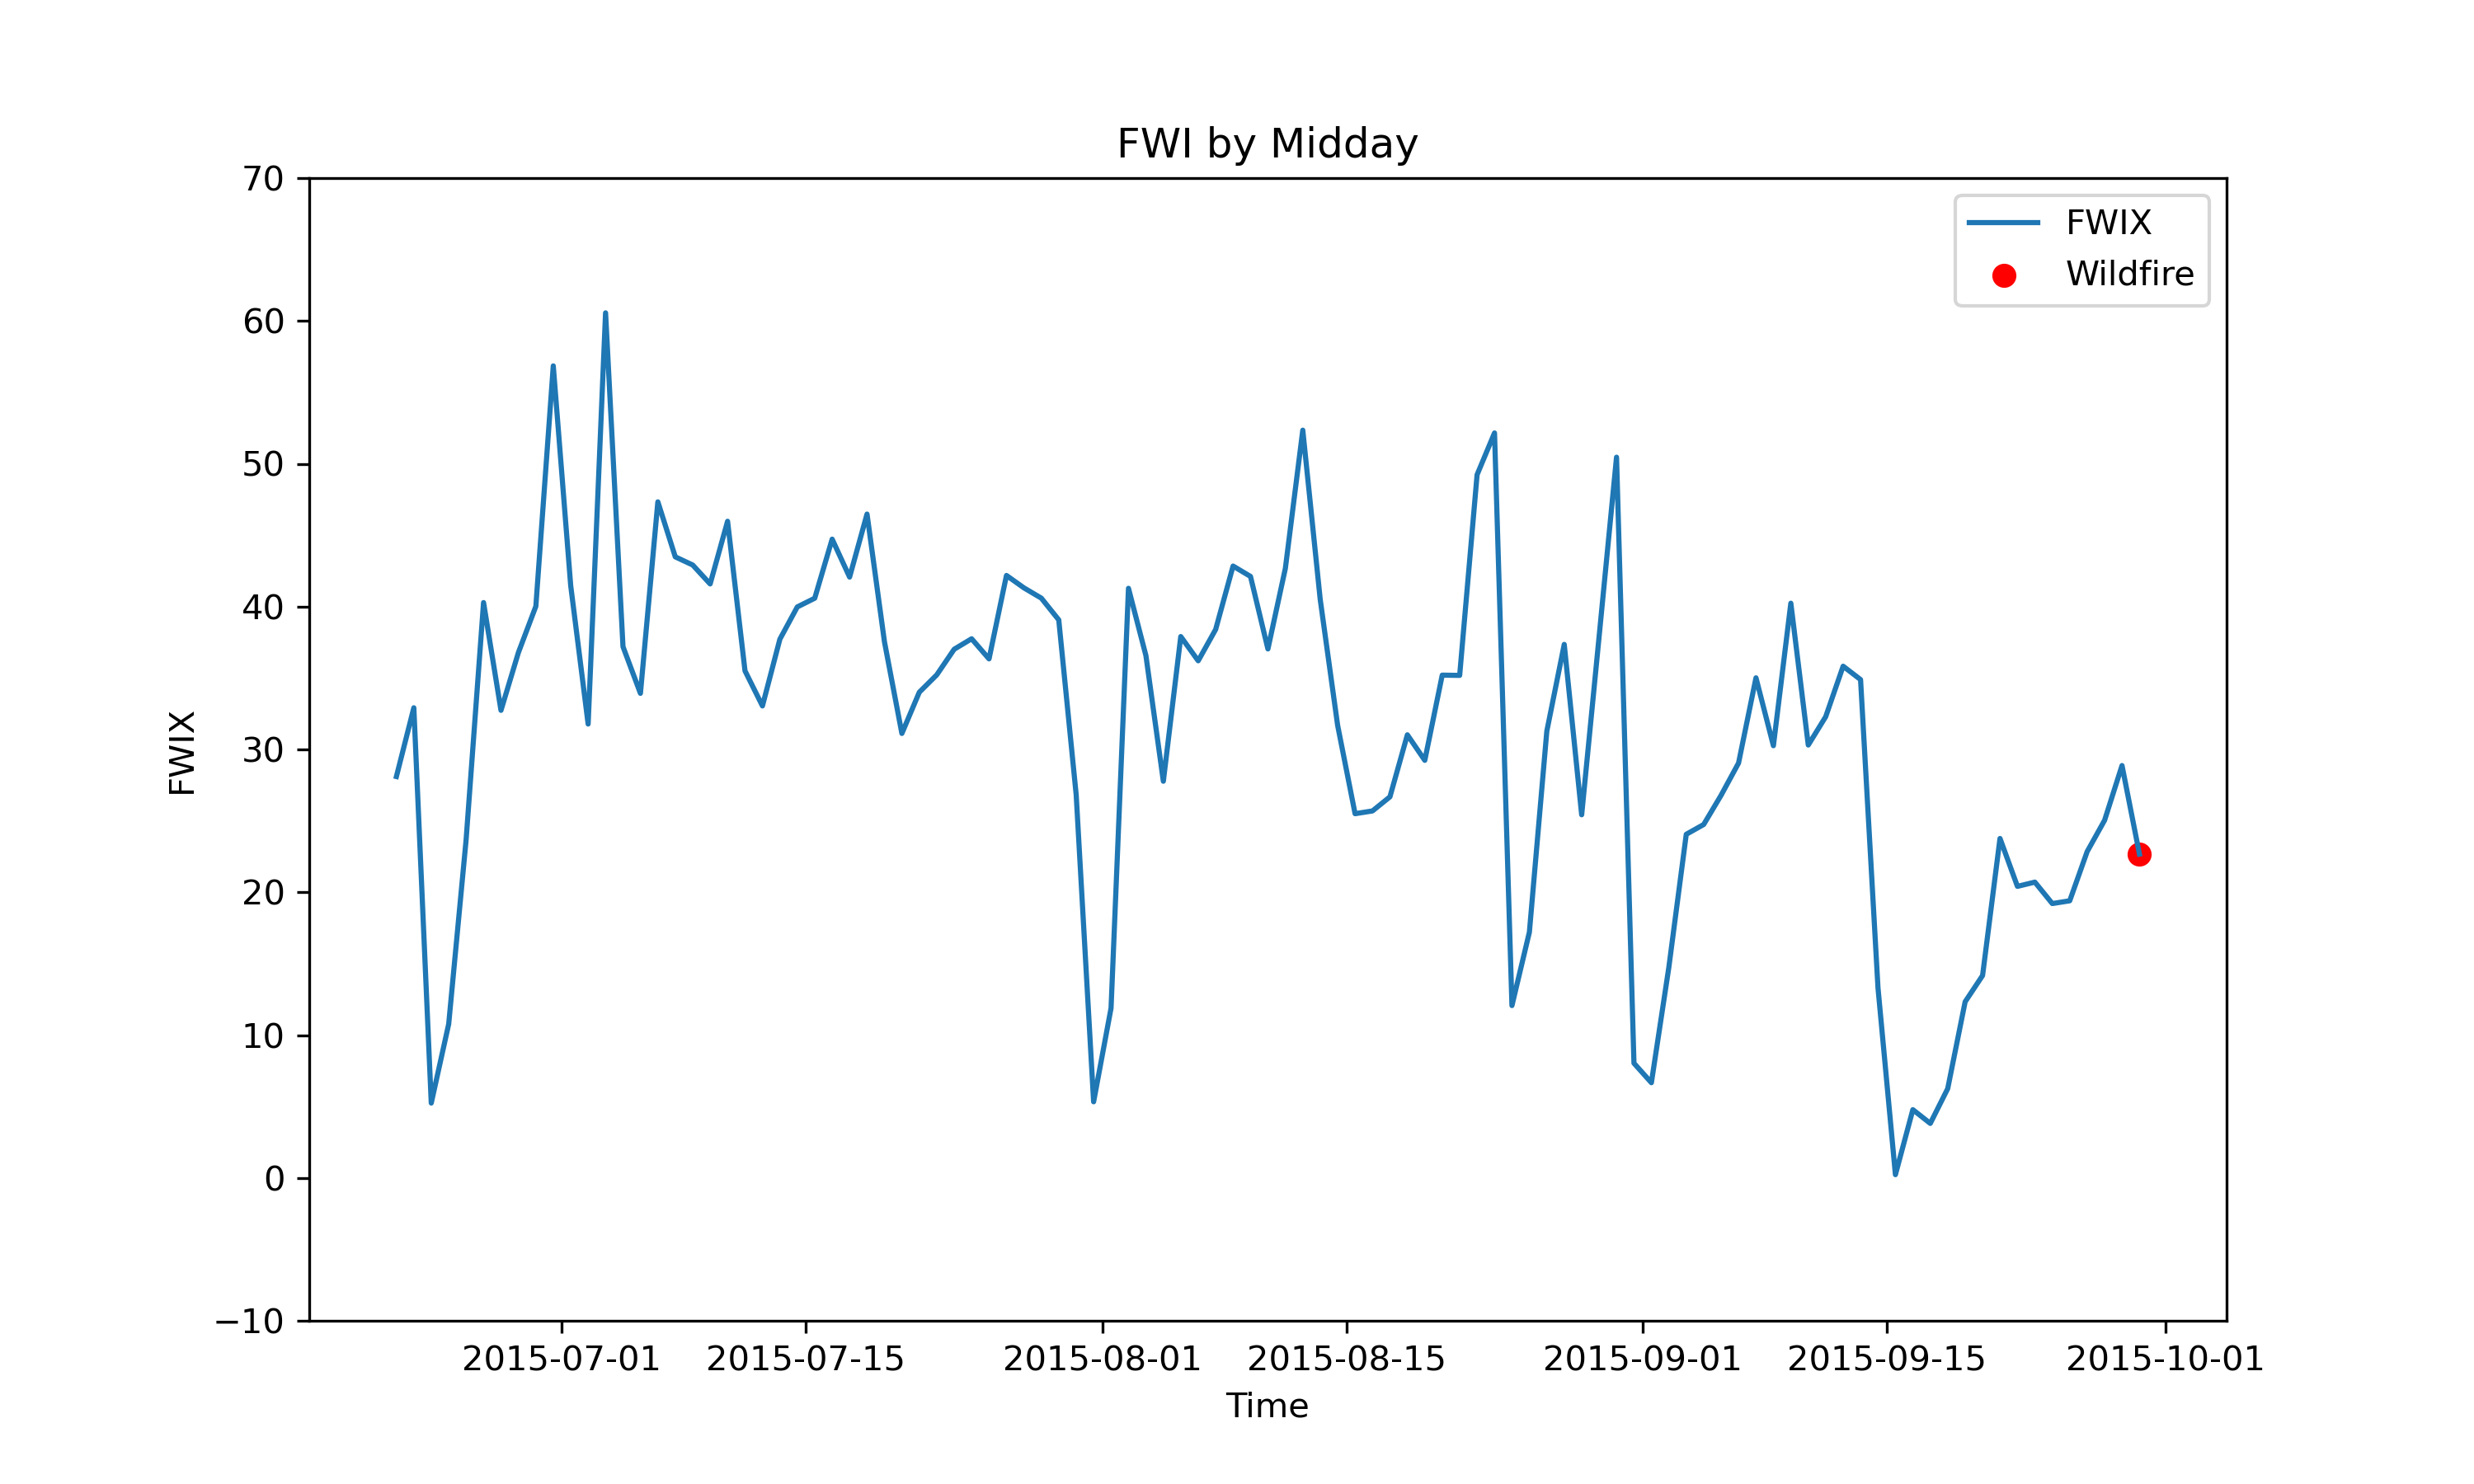
\includegraphics[width=\textwidth]{graphs/2015MesmoSitio/2015CalcFWI12.png}
        \caption{Caption for image 2}
        \label{fig:img2}
    \end{subfigure}
    \label{fig:both_images}
\end{figure}

\begin{figure}[h]
\caption{HELLo}
    \centering
    \begin{subfigure}{0.49\textwidth}
        \centering
        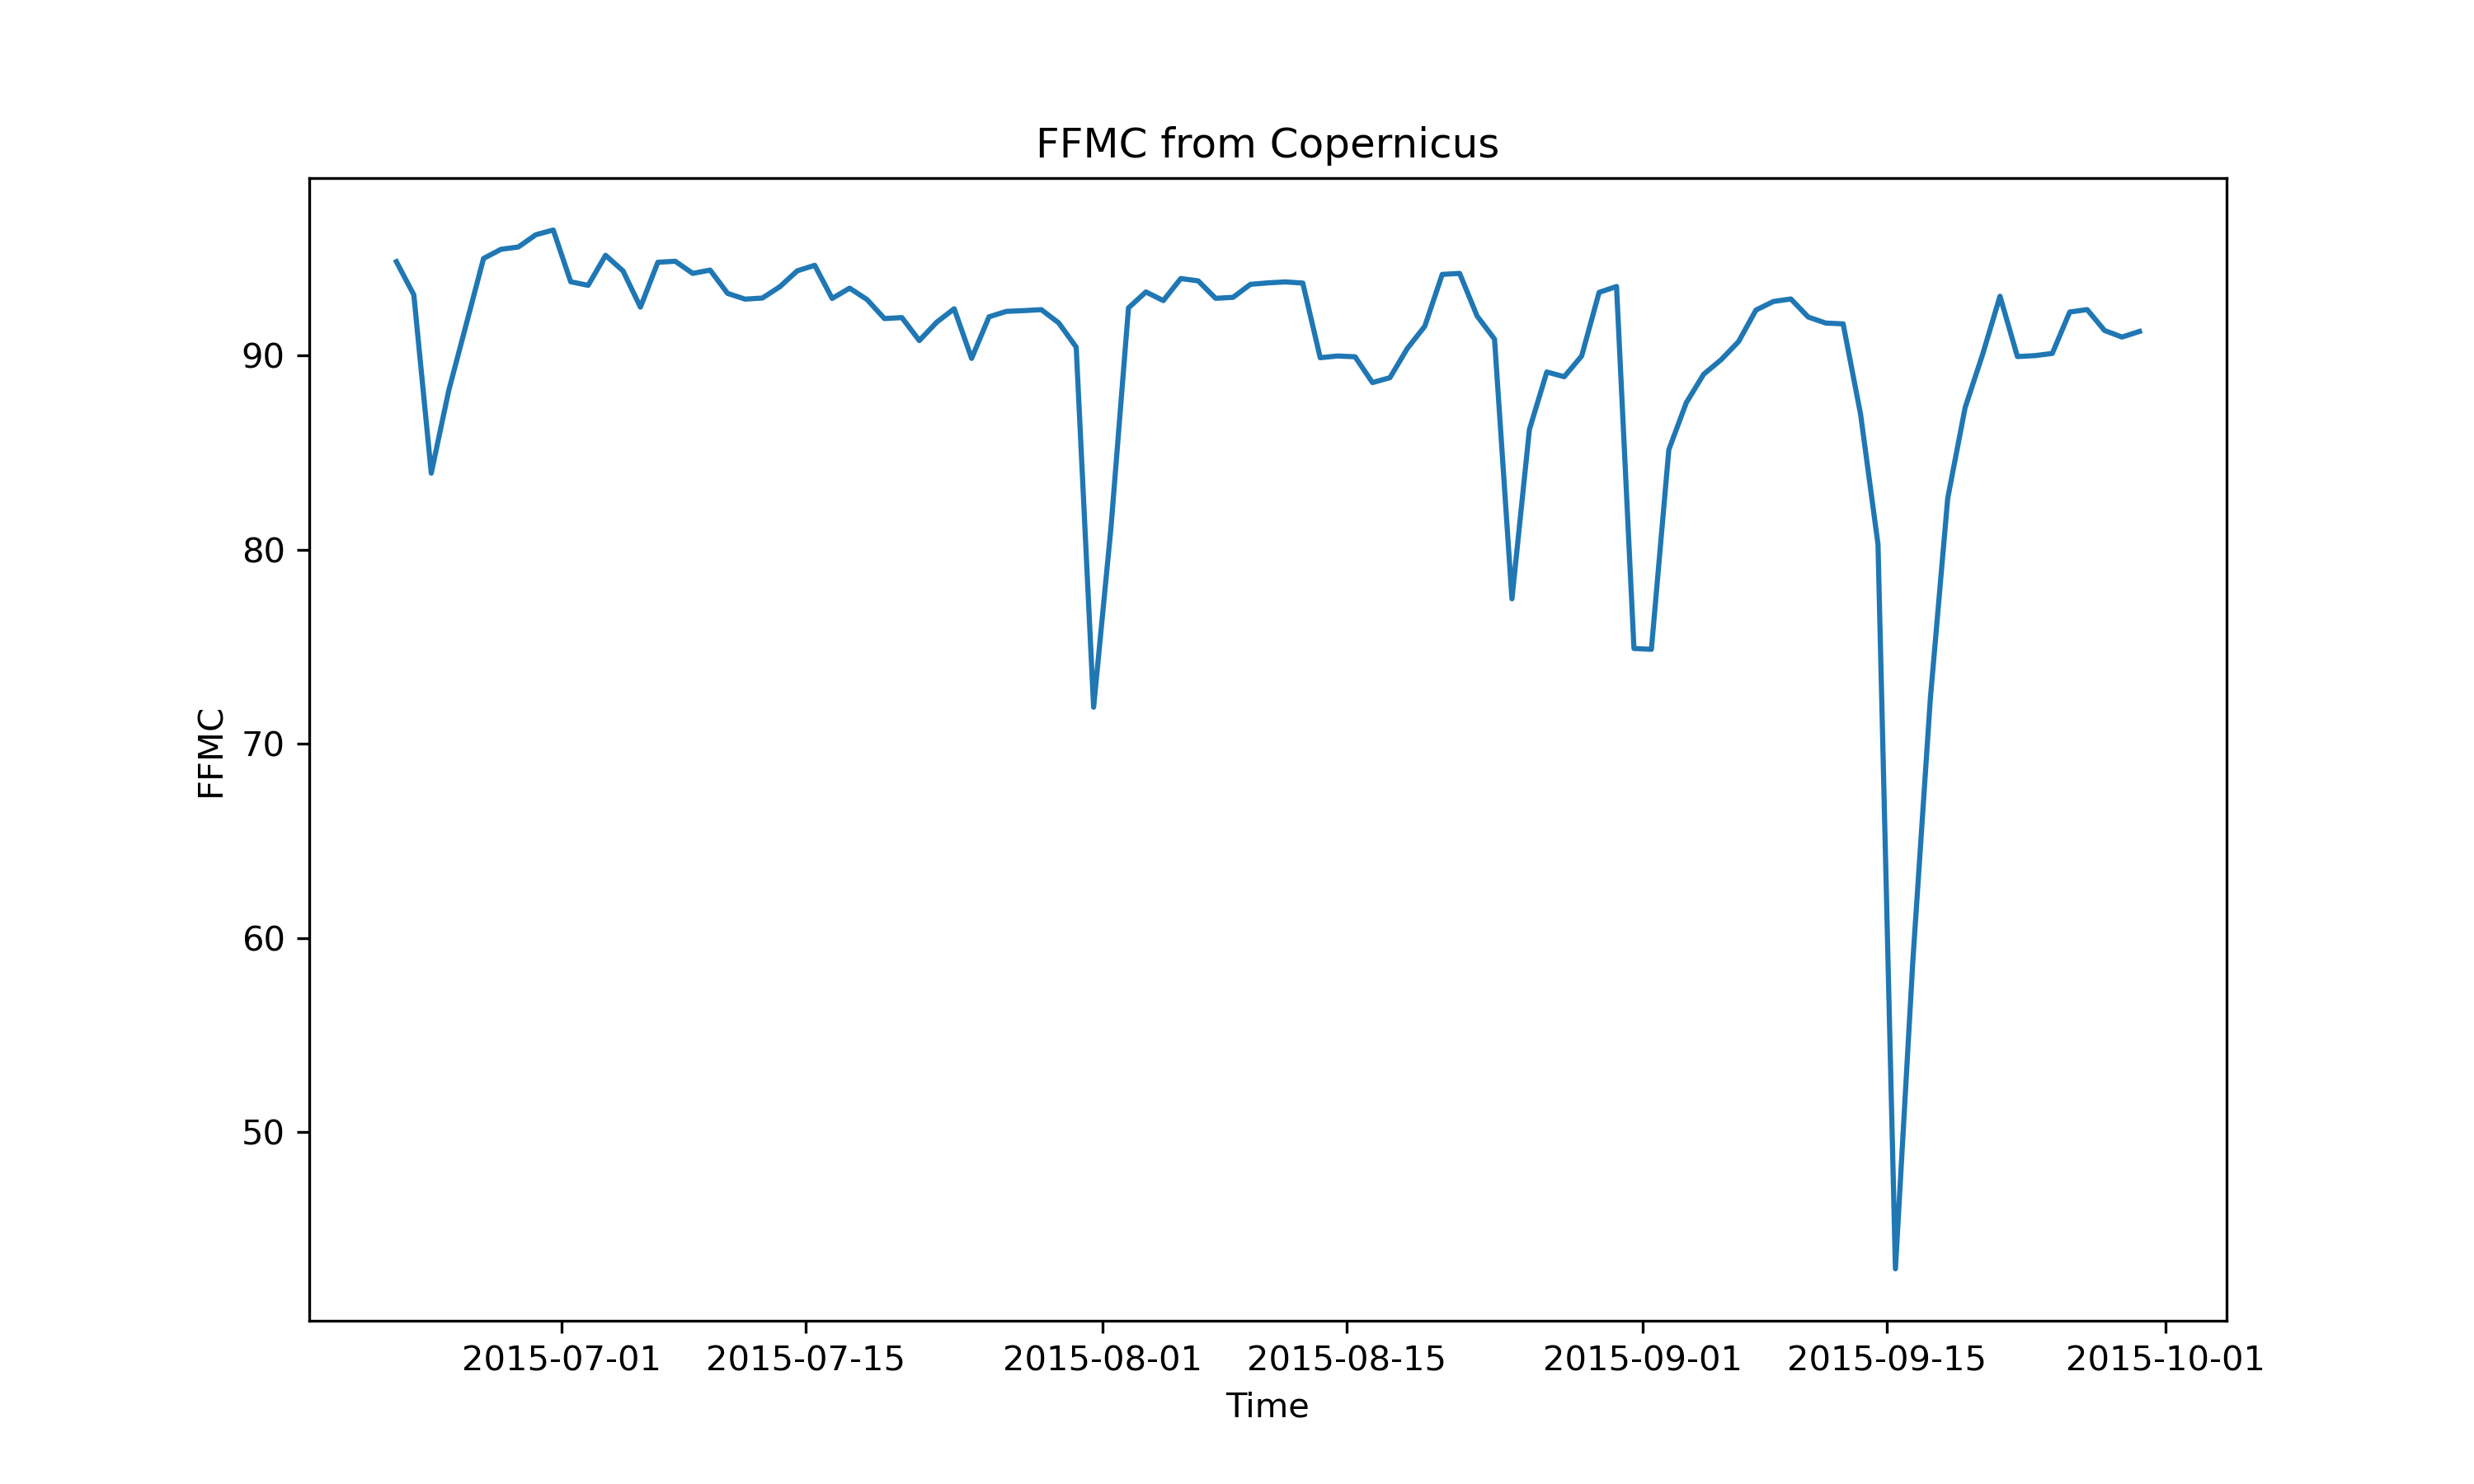
\includegraphics[width=\textwidth]{graphs/2015MesmoSitio/2015CopernicusFFMC12.png}
        \caption{Caption for image 1}
        \label{fig:img1}
    \end{subfigure}
    \hfill
    \begin{subfigure}{0.49\textwidth}
        \centering
        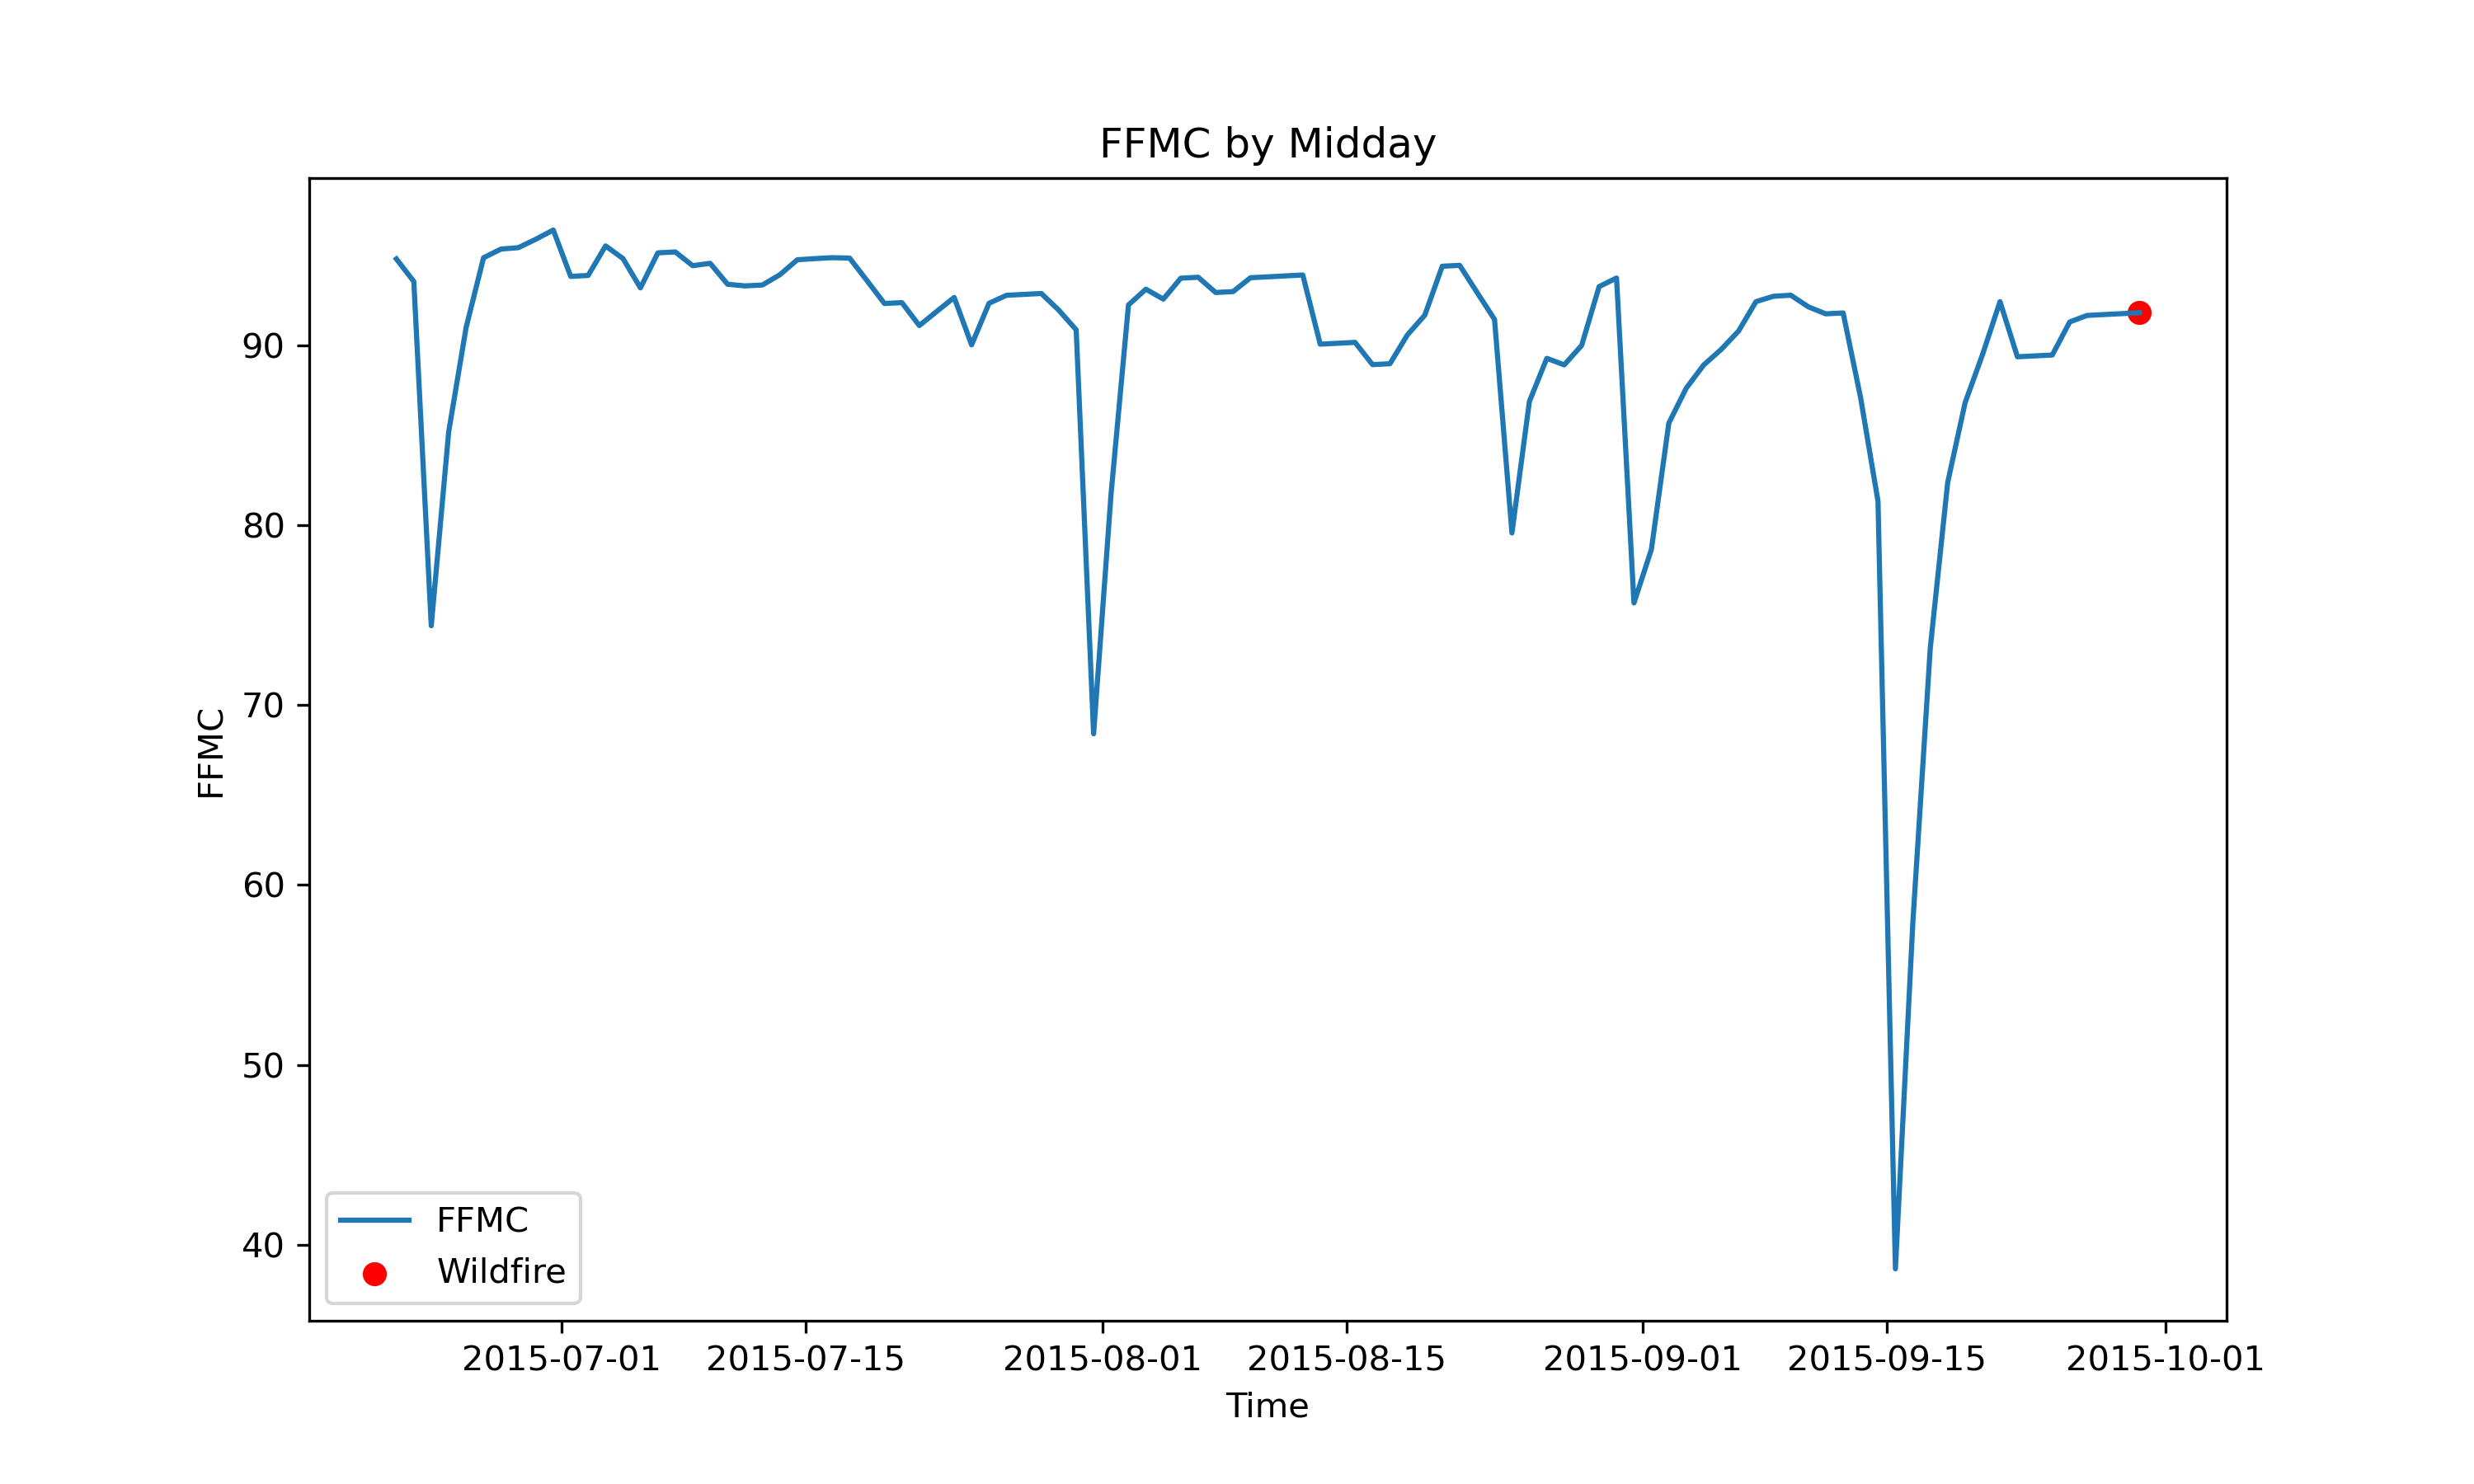
\includegraphics[width=\textwidth]{graphs/2015MesmoSitio/2015CalcFFMC12.png}
        \caption{Caption for image 2}
        \label{fig:img2}
    \end{subfigure}
    \label{fig:both_images}
\end{figure}

\begin{figure}[h]
\caption{HELLo}
    \centering
    \begin{subfigure}{0.49\textwidth}
        \centering
        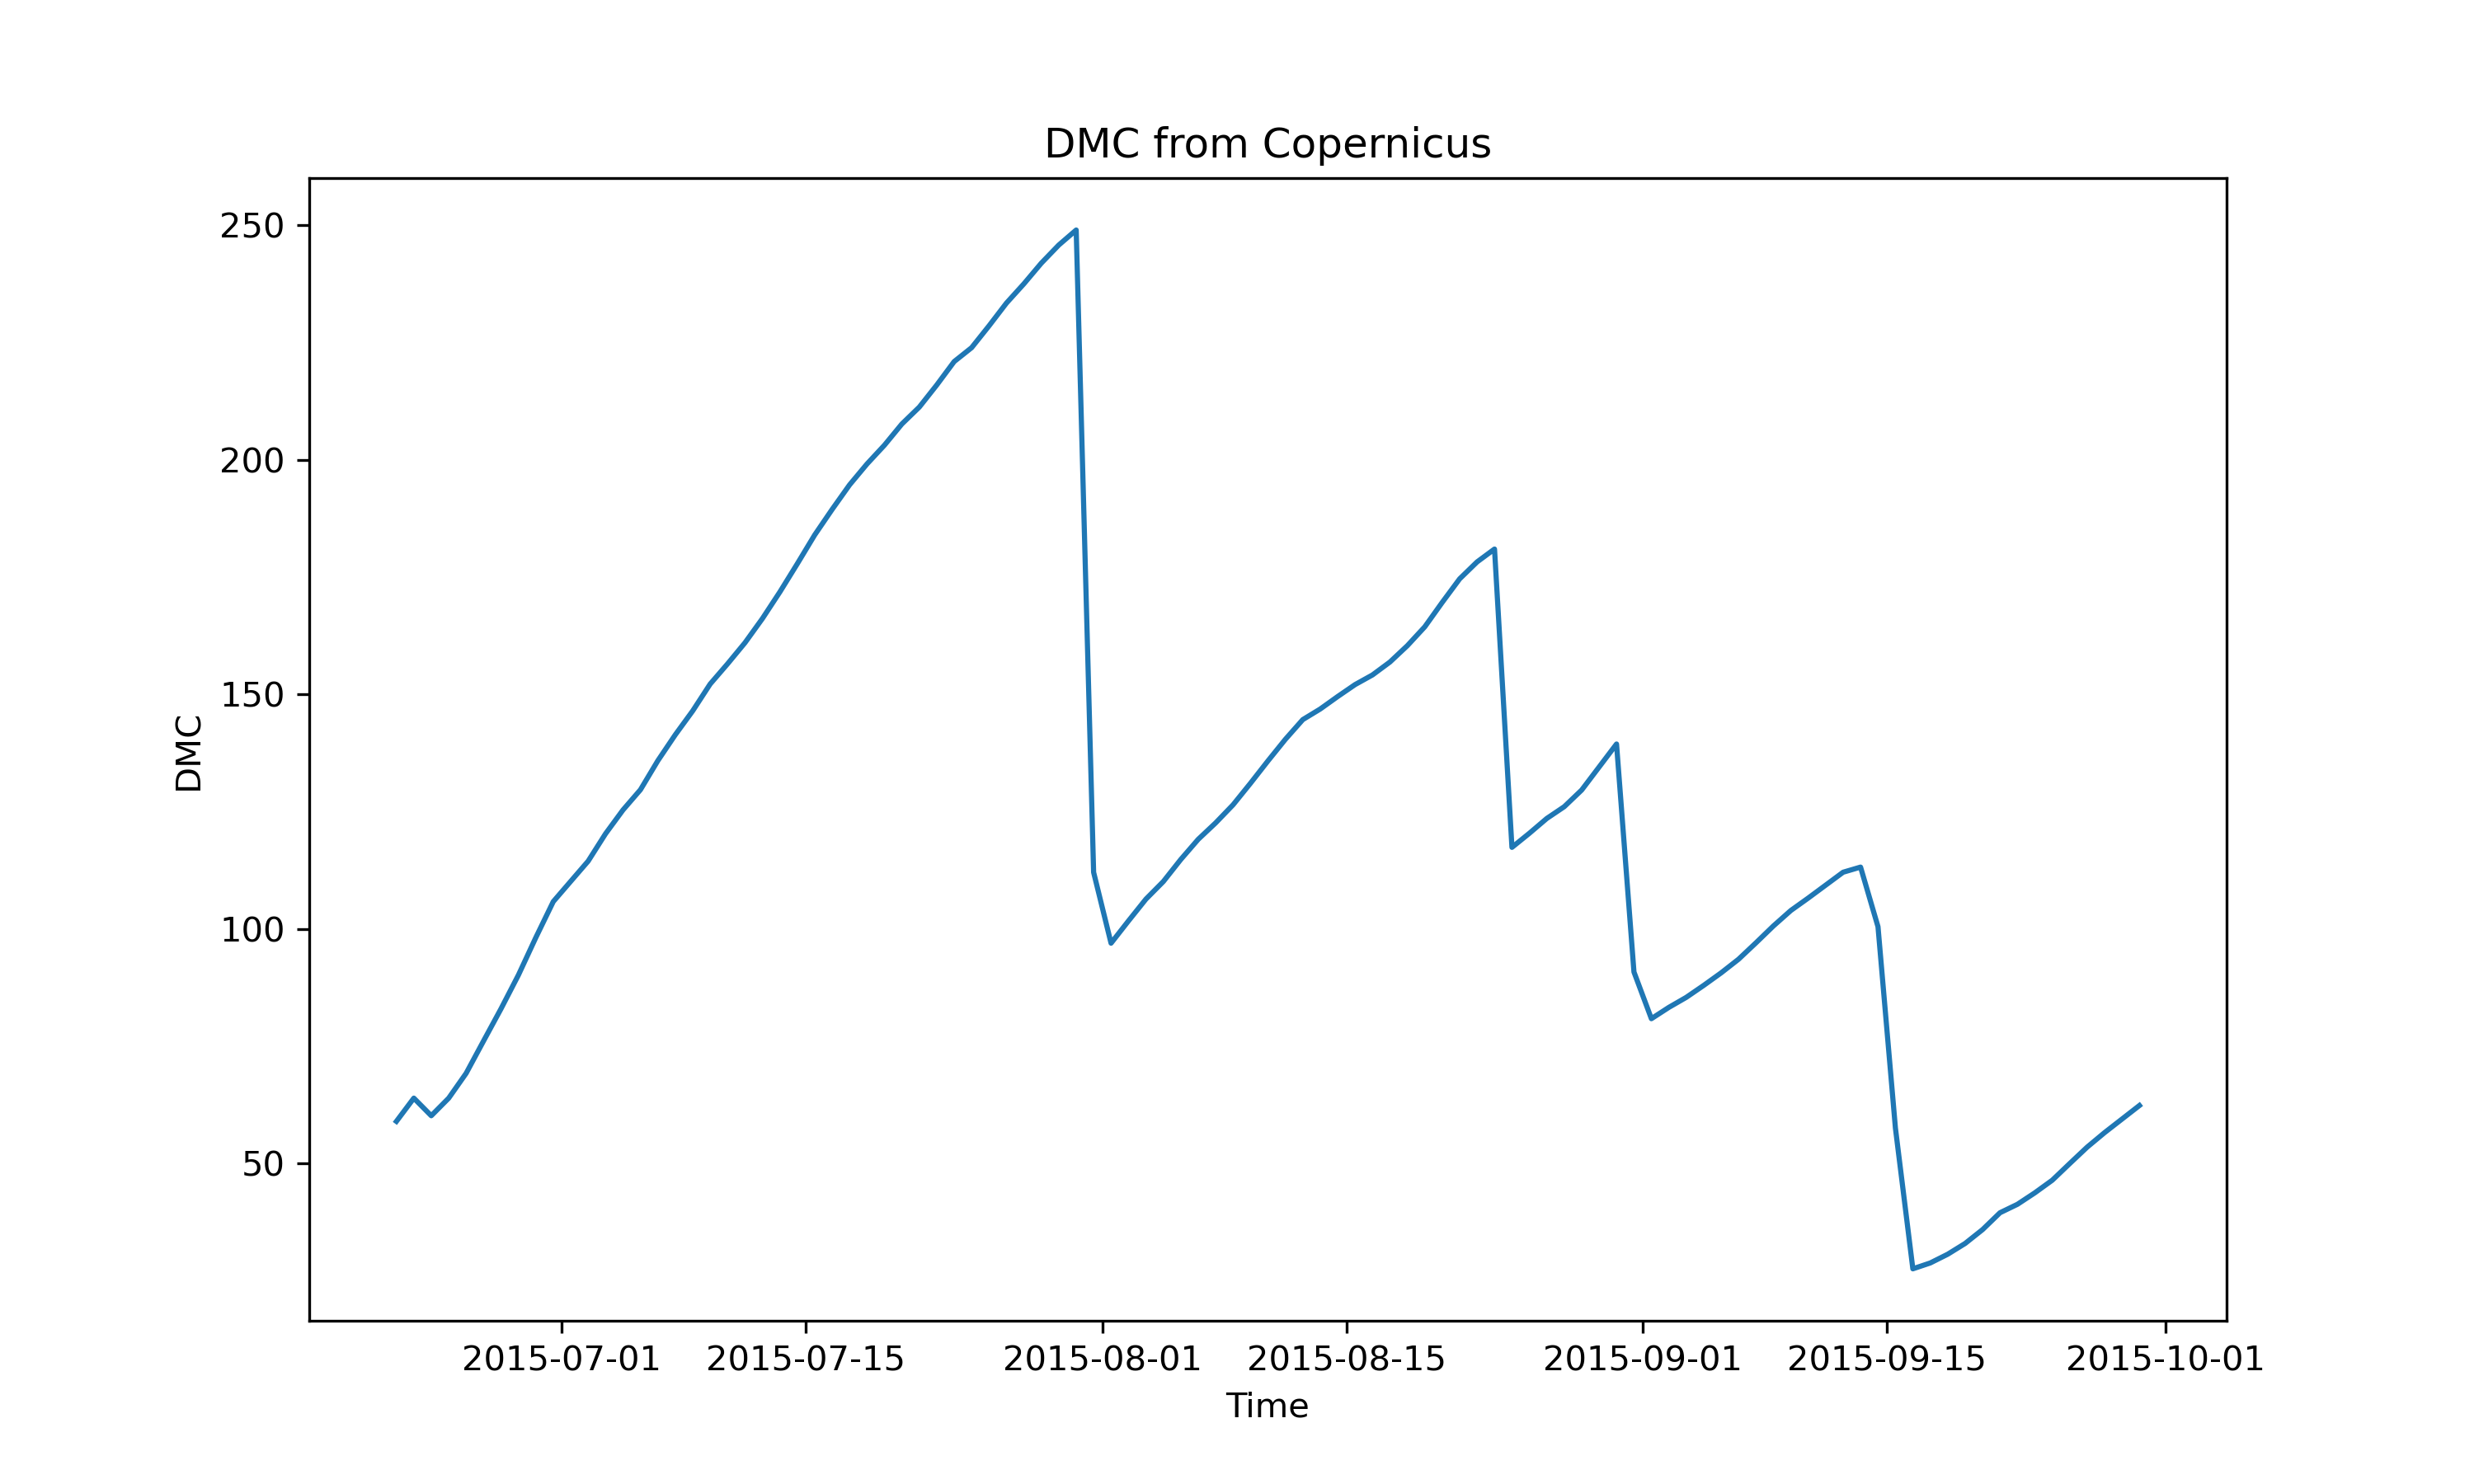
\includegraphics[width=\textwidth]{graphs/2015MesmoSitio/2015CopernicusDMC12.png}
        \caption{Caption for image 1}
        \label{fig:img1}
    \end{subfigure}
    \hfill
    \begin{subfigure}{0.49\textwidth}
        \centering
        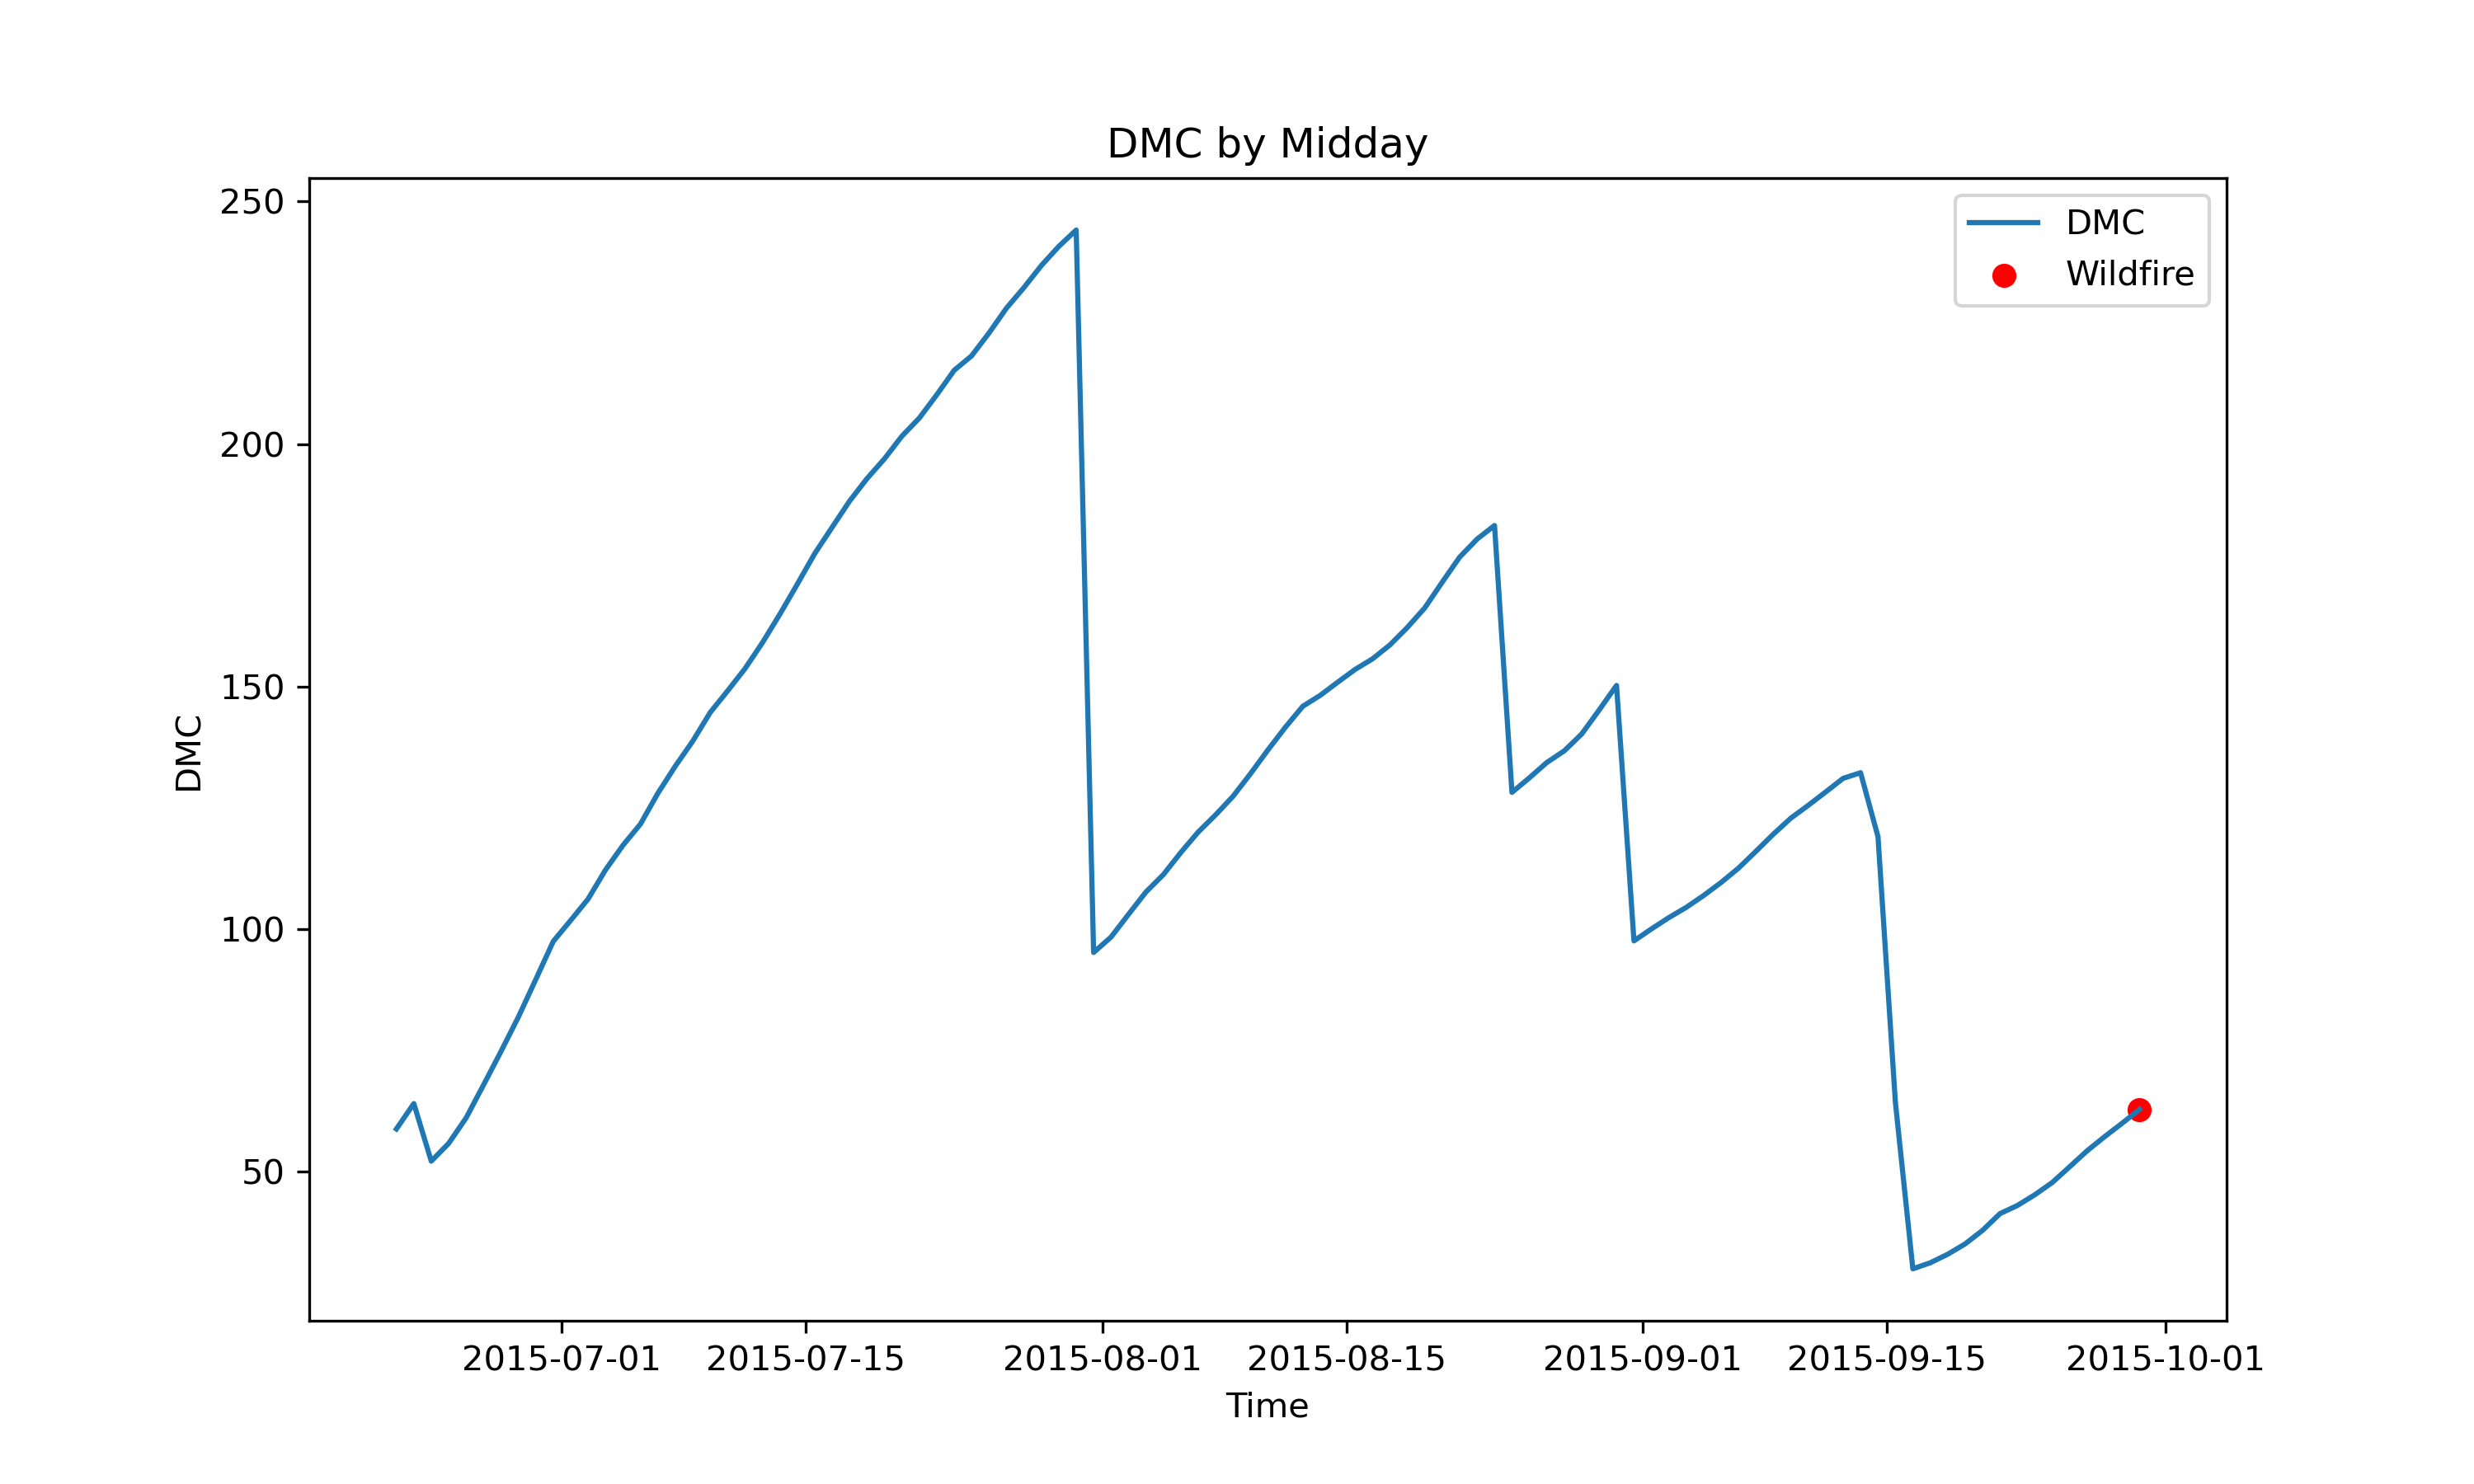
\includegraphics[width=\textwidth]{graphs/2015MesmoSitio/2015CalcDMC12.png}
        \caption{Caption for image 2}
        \label{fig:img2}
    \end{subfigure}
    \label{fig:both_images}
\end{figure}

\begin{figure}[h]
\caption{HELLo}
    \centering
    \begin{subfigure}{0.49\textwidth}
        \centering
        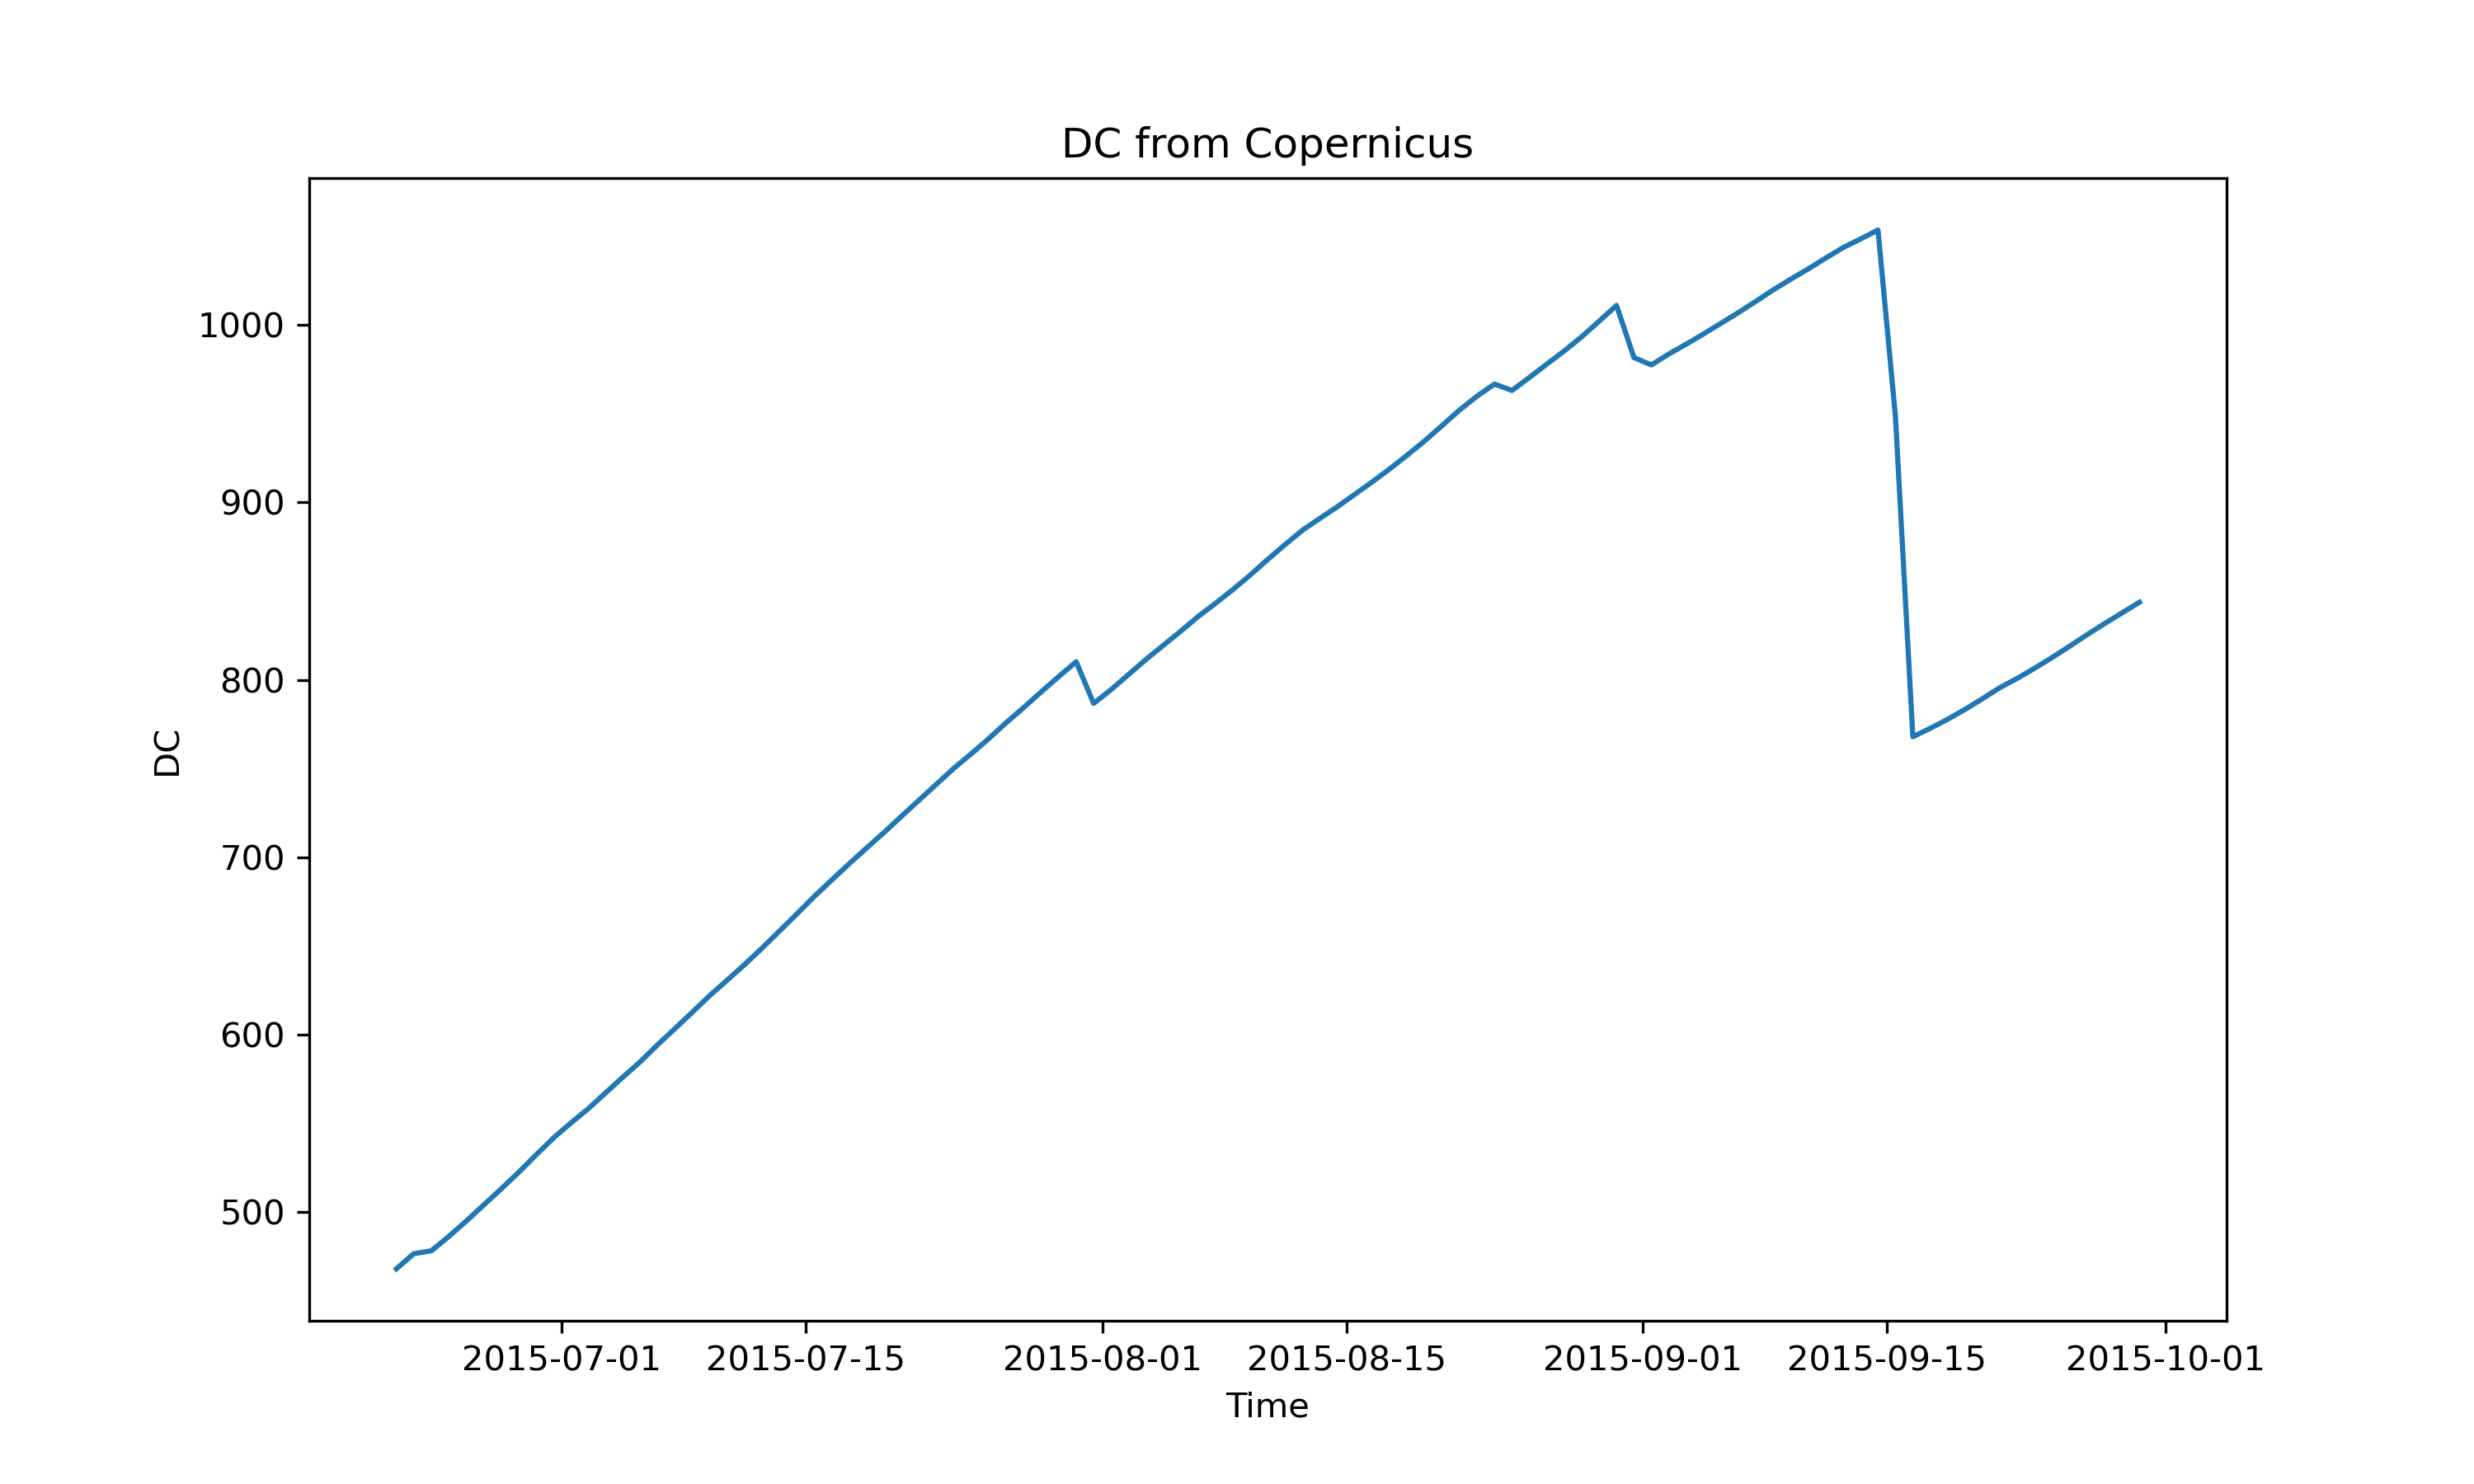
\includegraphics[width=\textwidth]{graphs/2015MesmoSitio/2015CopernicusDC12.png}
        \caption{Caption for image 1}
        \label{fig:img1}
    \end{subfigure}
    \hfill
    \begin{subfigure}{0.49\textwidth}
        \centering
        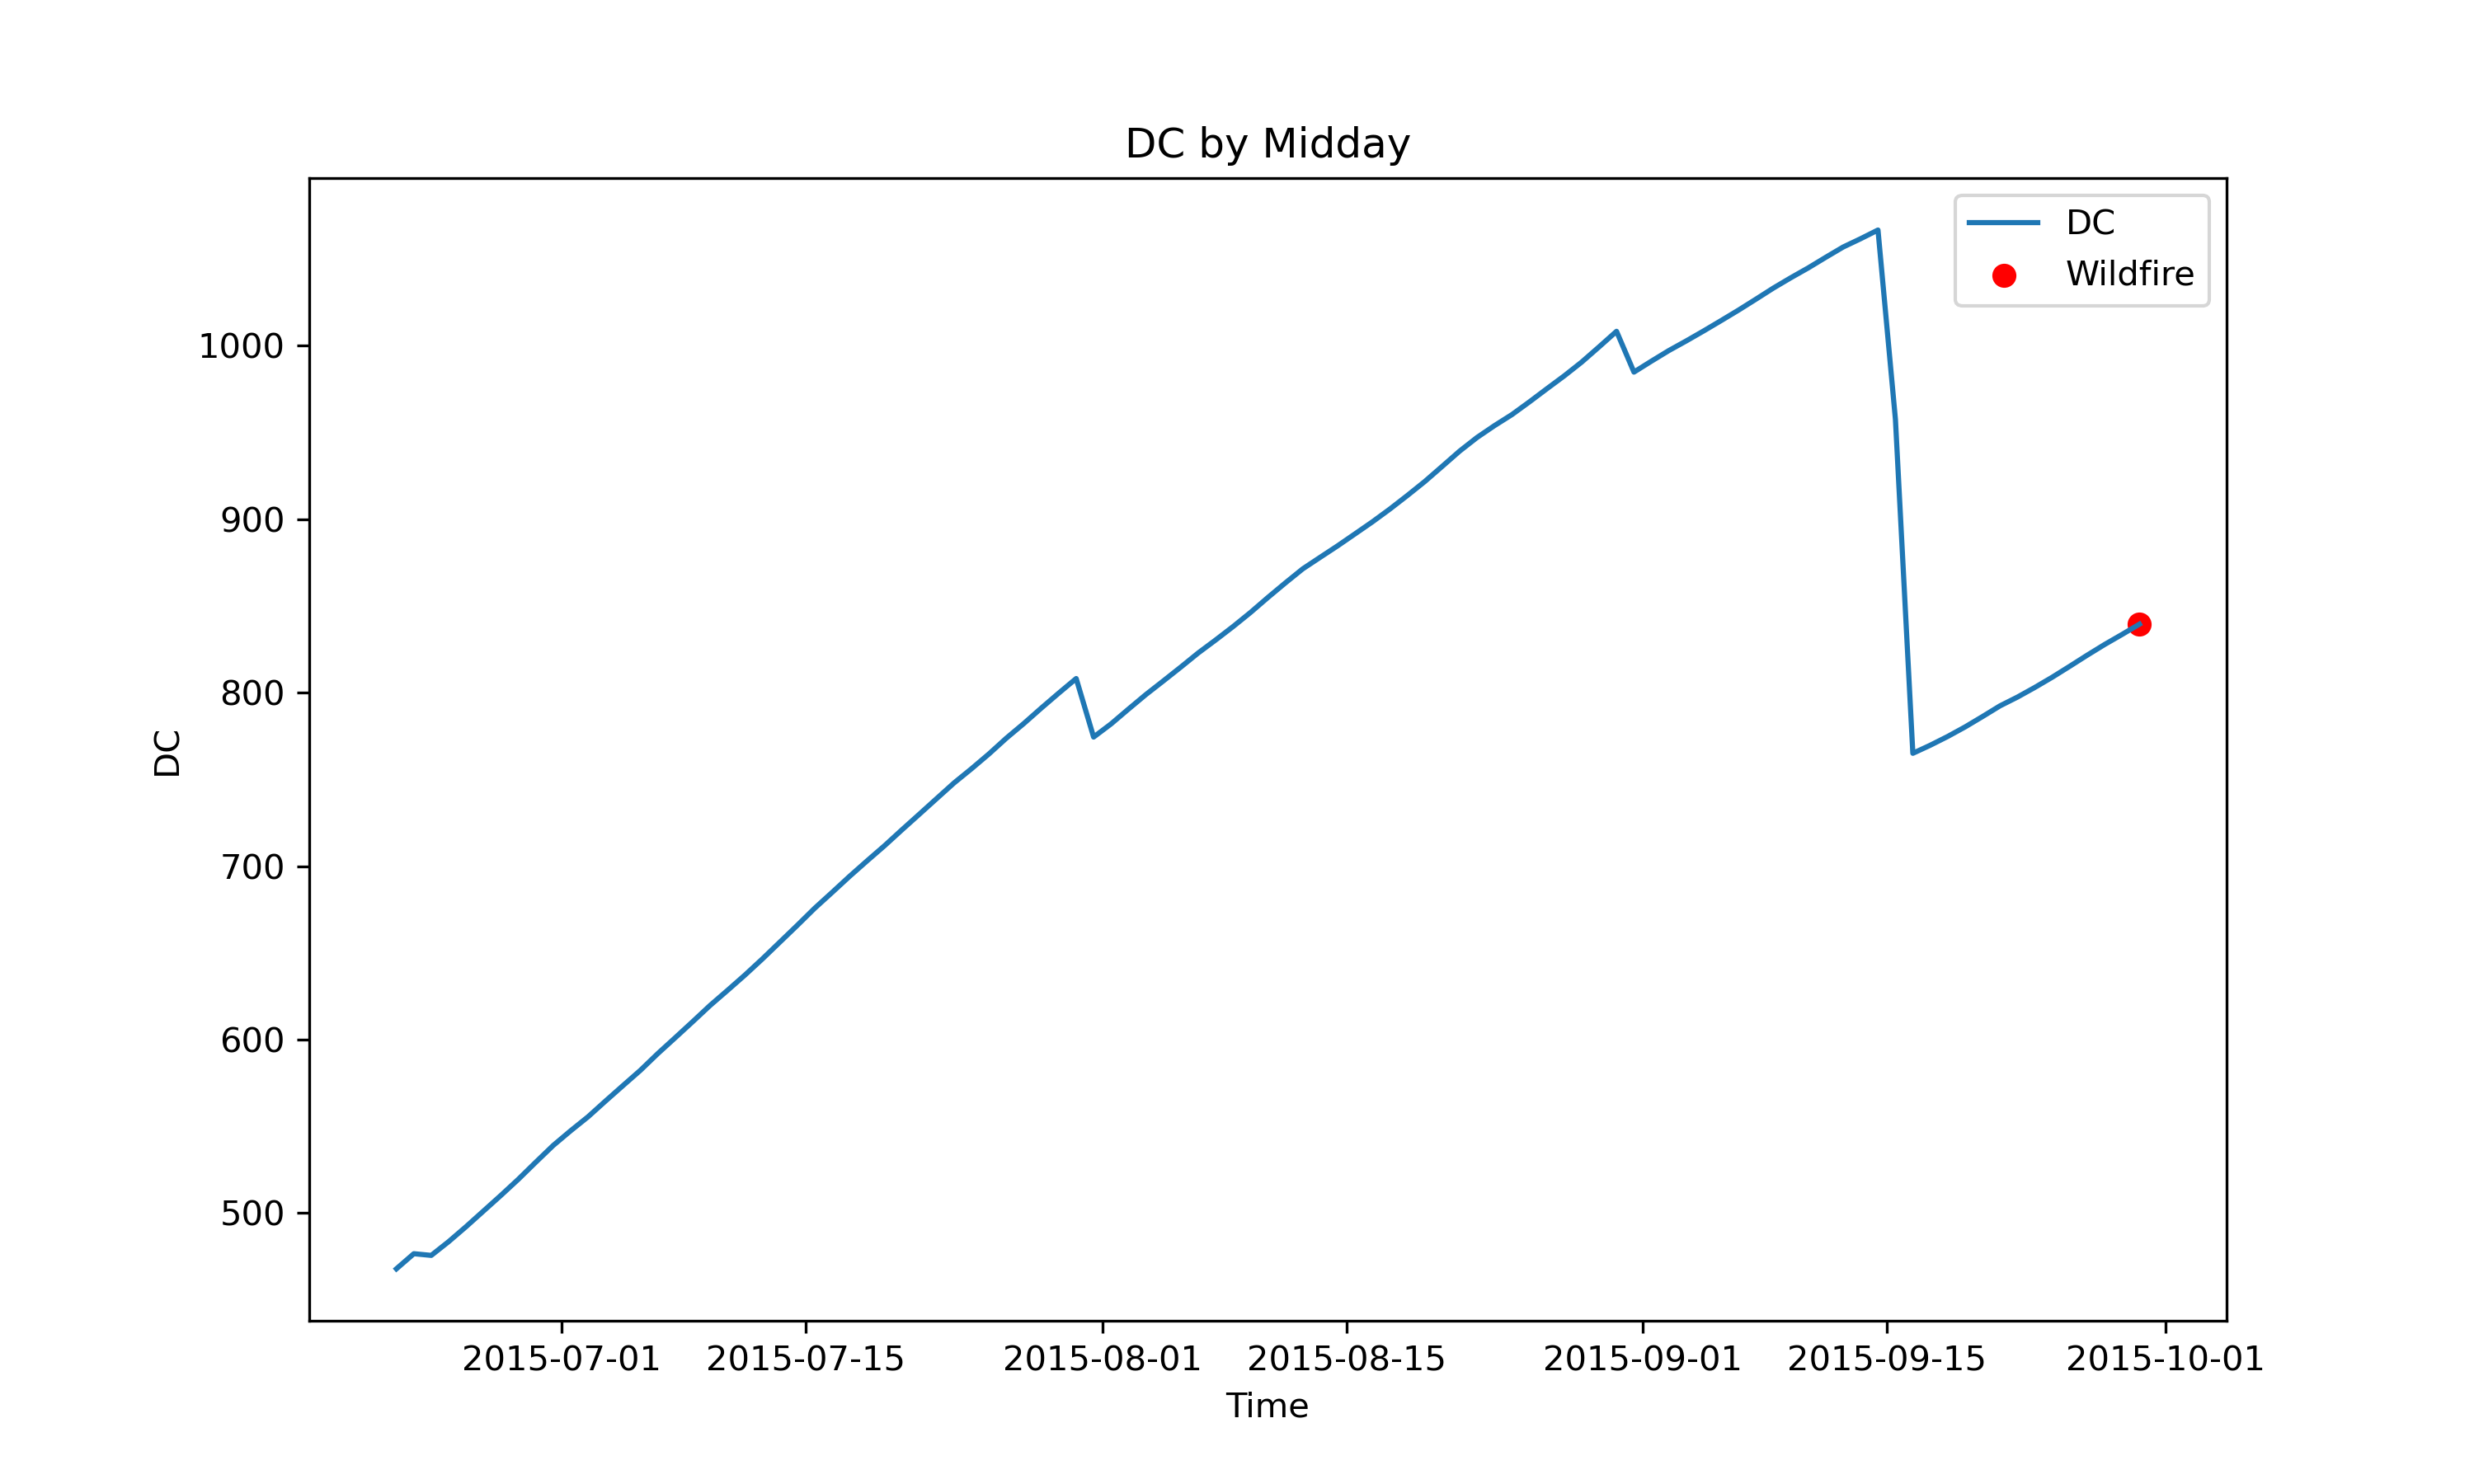
\includegraphics[width=\textwidth]{graphs/2015MesmoSitio/2015CalcDC12.png}
        \caption{Caption for image 2}
        \label{fig:img2}
    \end{subfigure}
    \label{fig:both_images}
\end{figure}

\begin{figure}[h]
\caption{HELLo}
    \centering
    \begin{subfigure}{0.49\textwidth}
        \centering
        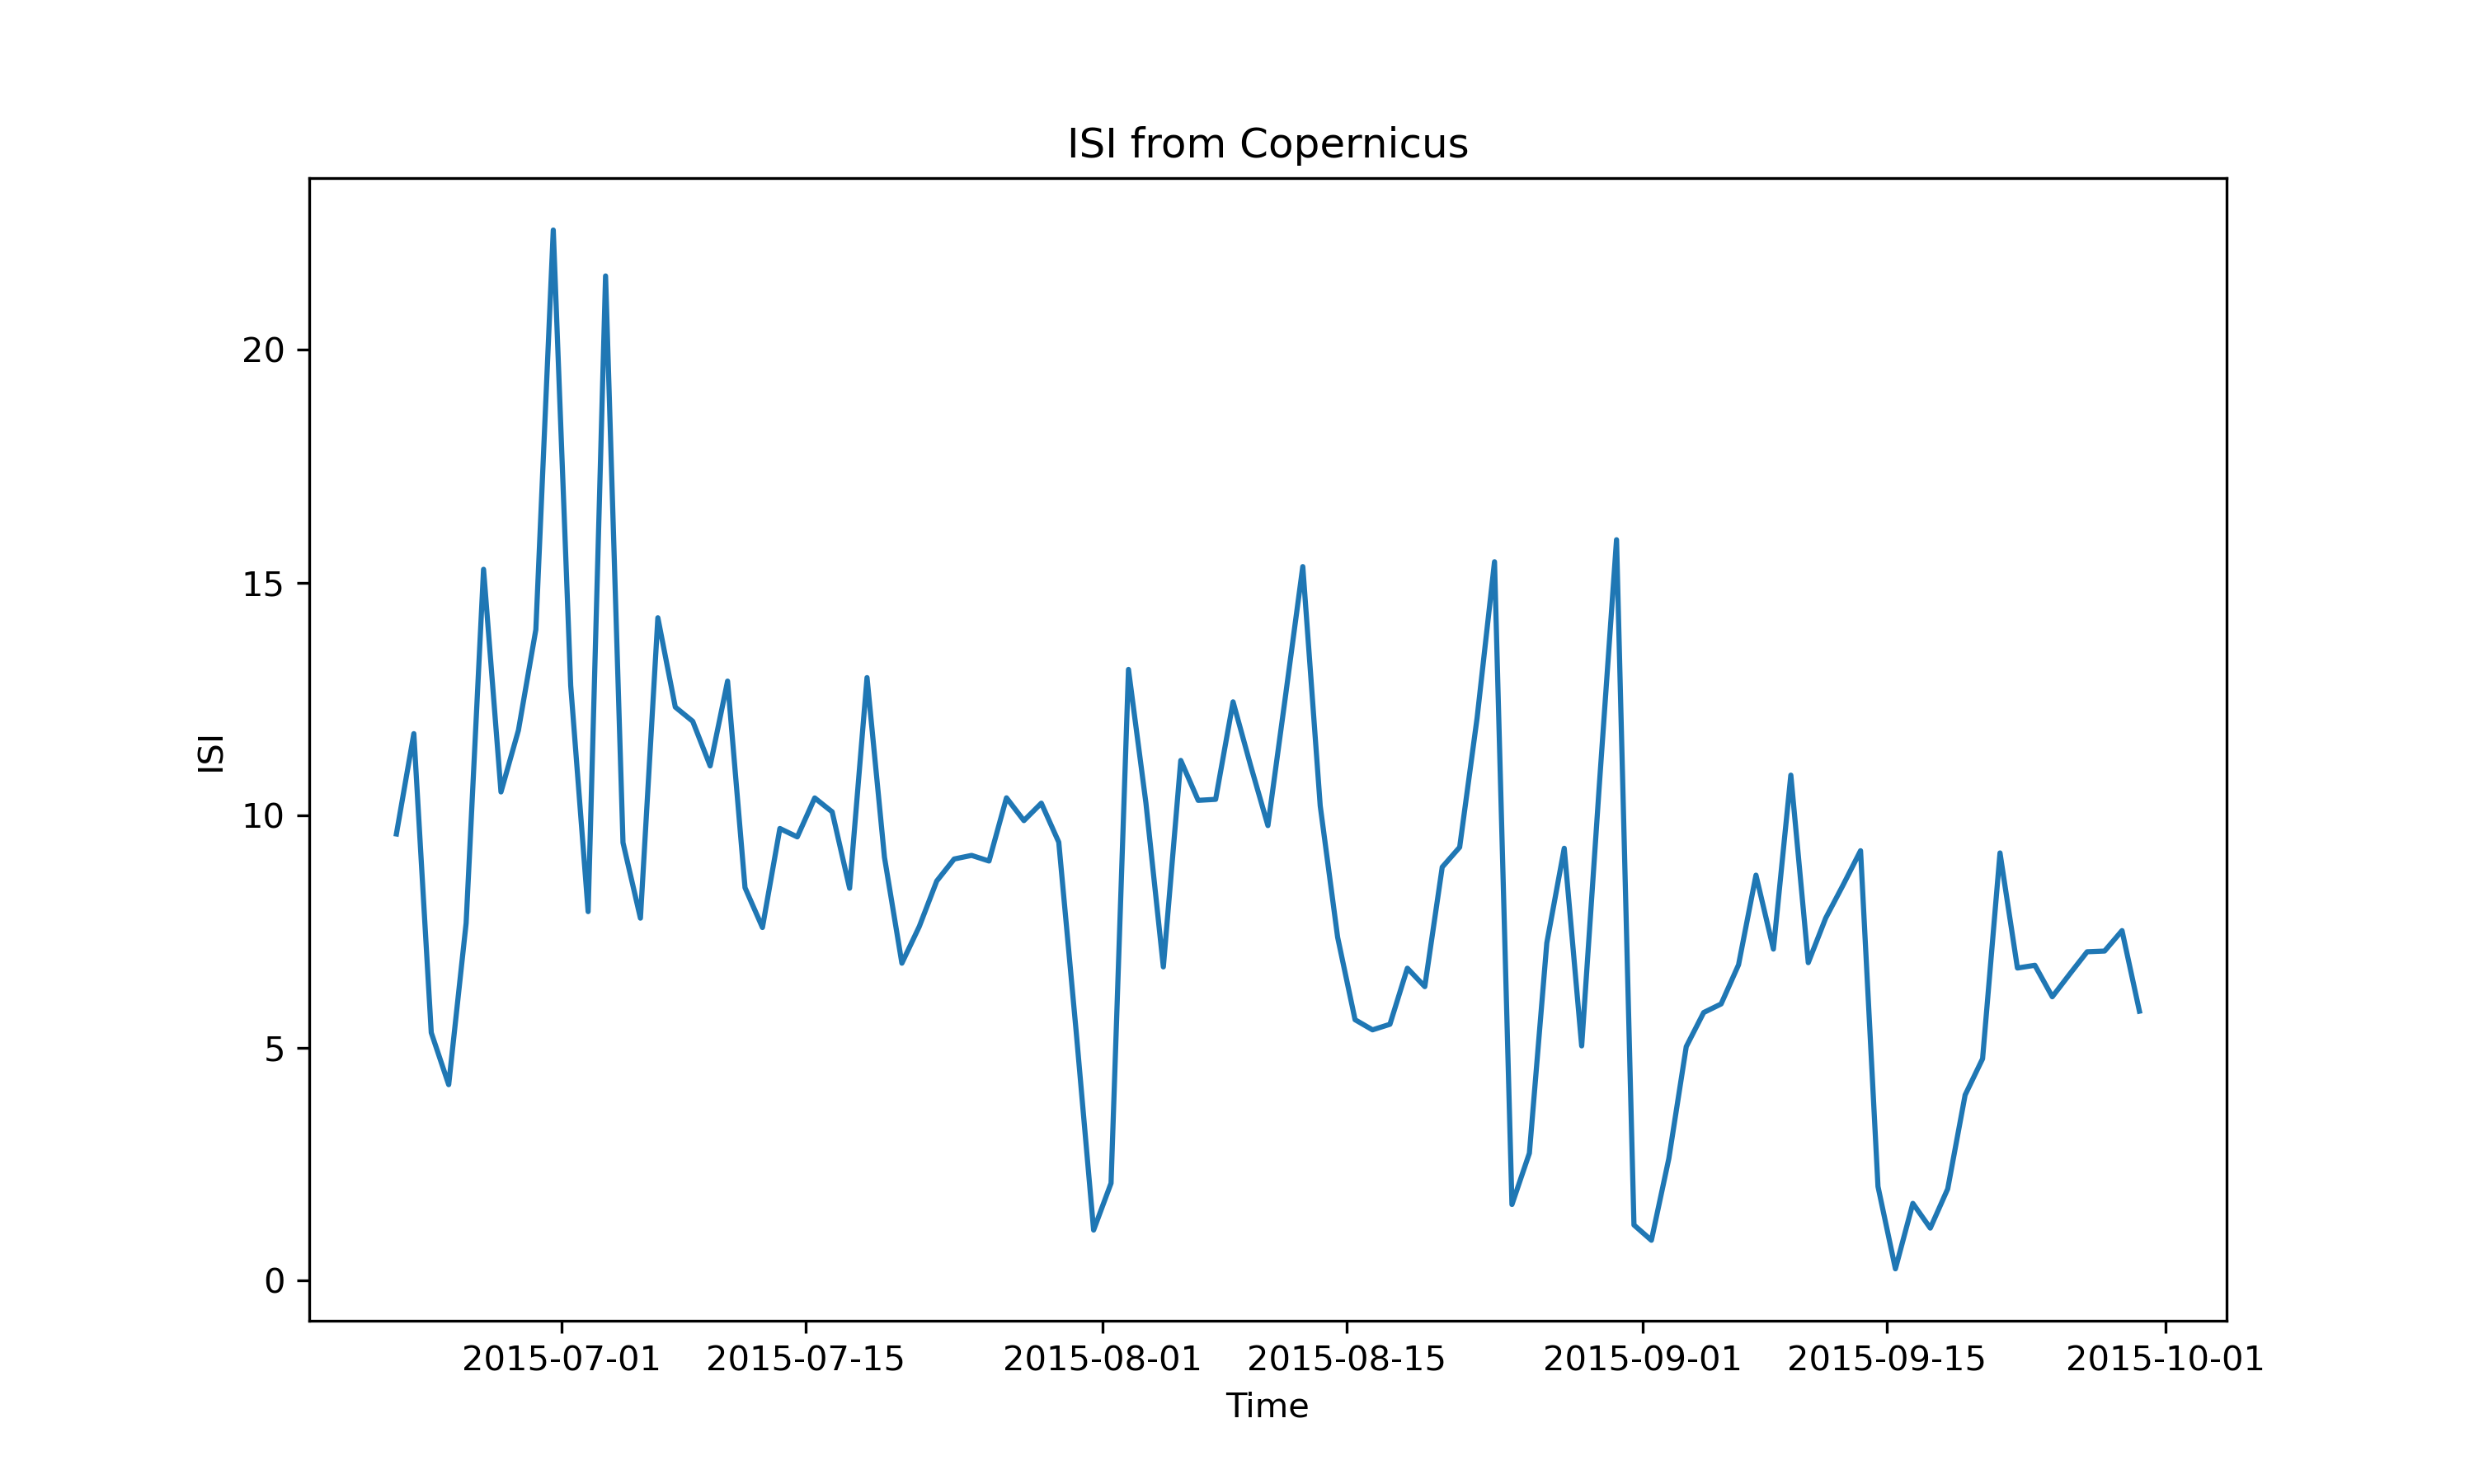
\includegraphics[width=\textwidth]{graphs/2015MesmoSitio/2015CopernicusISI12.png}
        \caption{Caption for image 1}
        \label{fig:img1}
    \end{subfigure}
    \hfill
    \begin{subfigure}{0.49\textwidth}
        \centering
        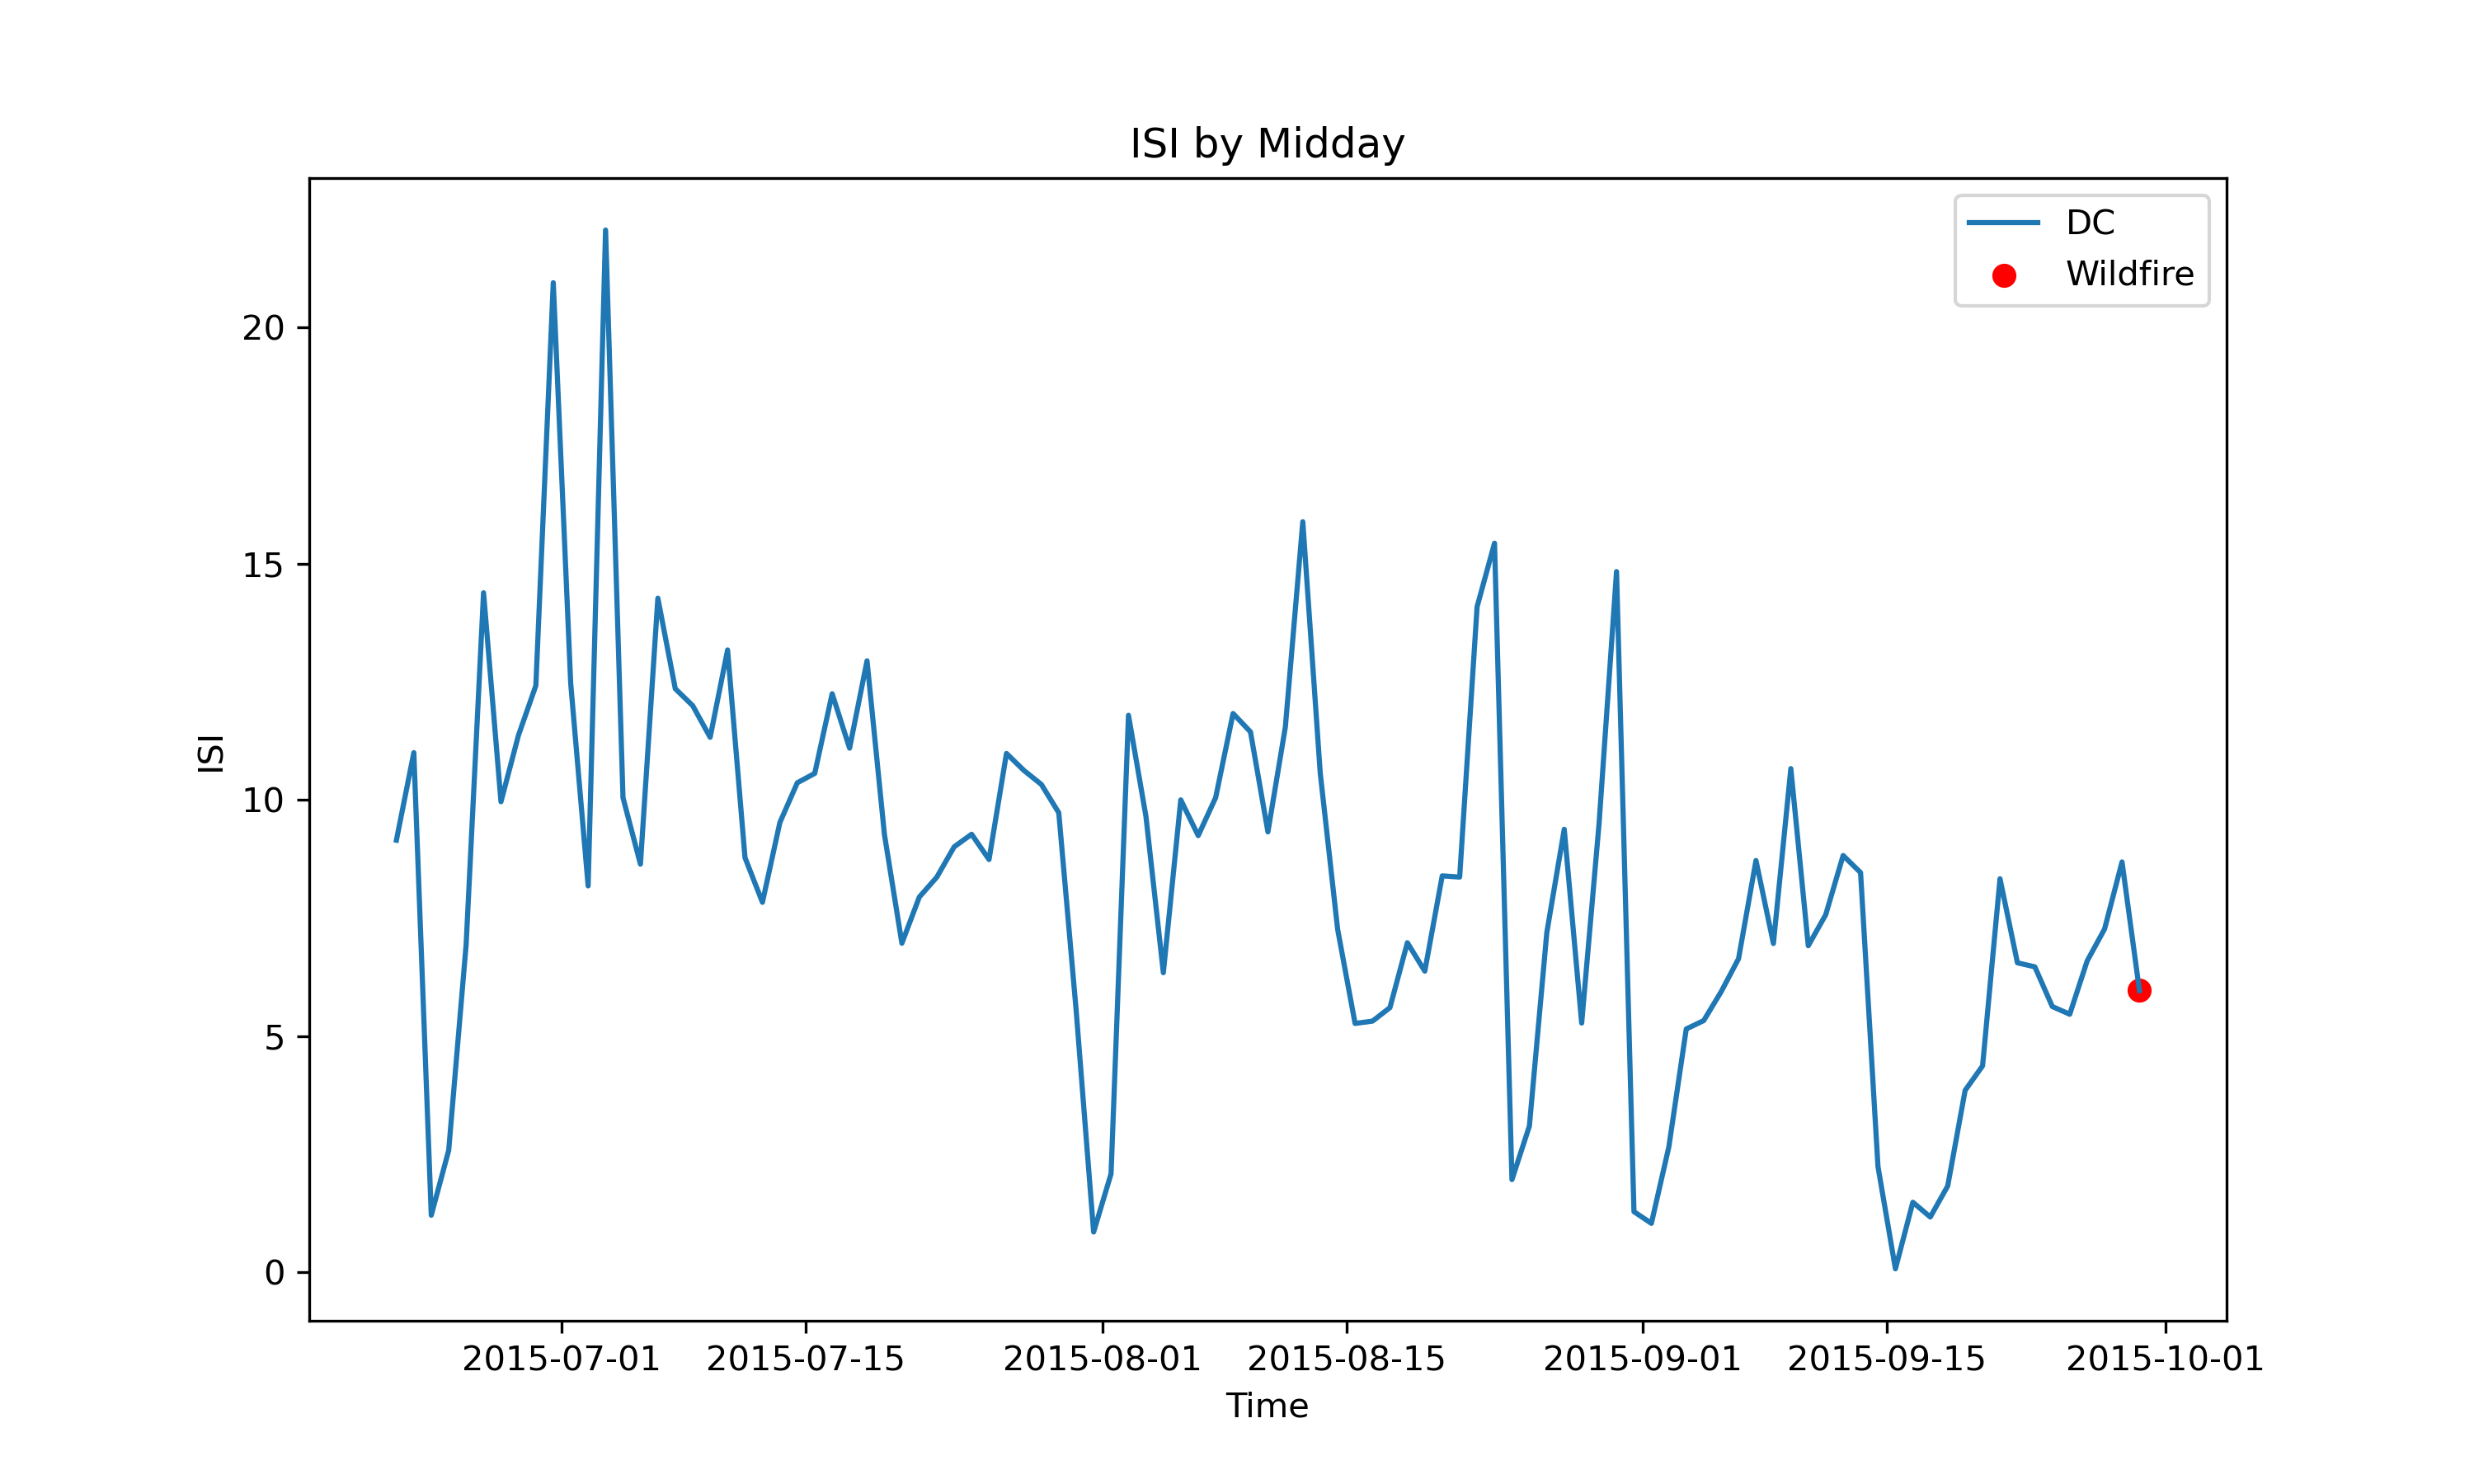
\includegraphics[width=\textwidth]{graphs/2015MesmoSitio/2015CalcISI12.png}
        \caption{Caption for image 2}
        \label{fig:img2}
    \end{subfigure}
    \label{fig:both_images}
\end{figure}

\begin{figure}[h]
\caption{HELLo}
    \centering
    \begin{subfigure}{0.49\textwidth}
        \centering
        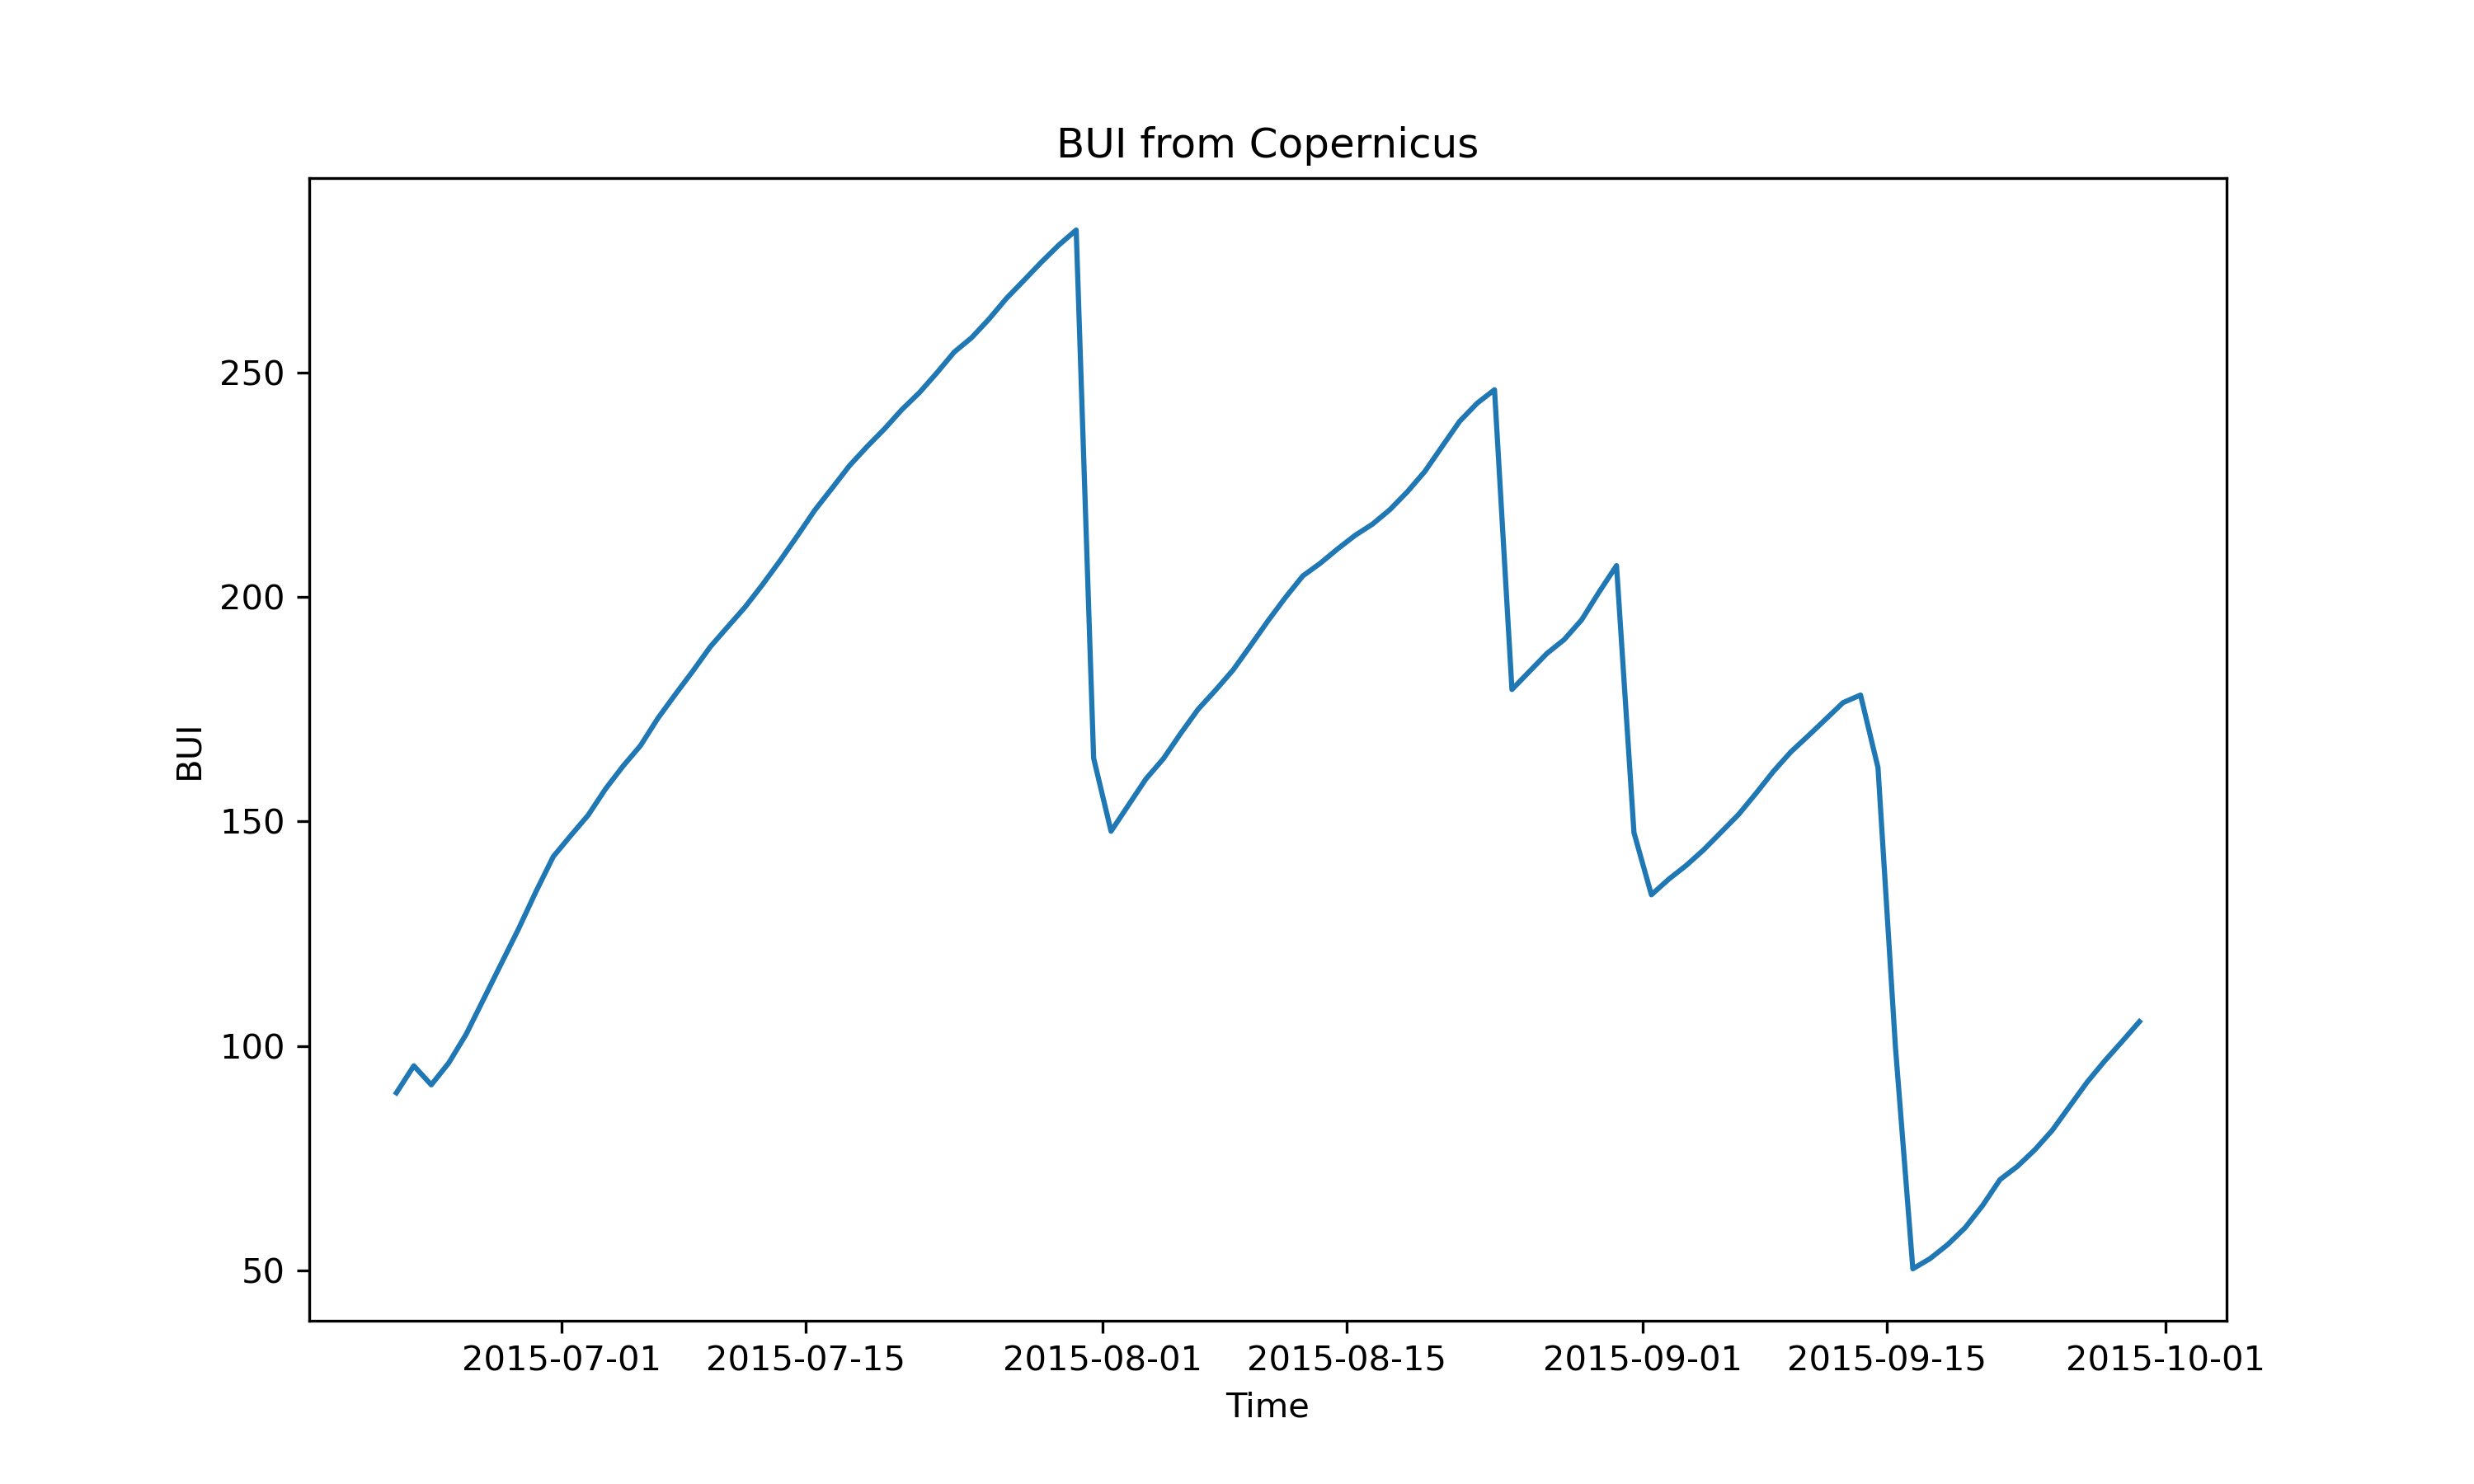
\includegraphics[width=\textwidth]{graphs/2015MesmoSitio/2015CopernicusBUI12.png}
        \caption{Caption for image 1}
        \label{fig:img1}
    \end{subfigure}
    \hfill
    \begin{subfigure}{0.49\textwidth}
        \centering
        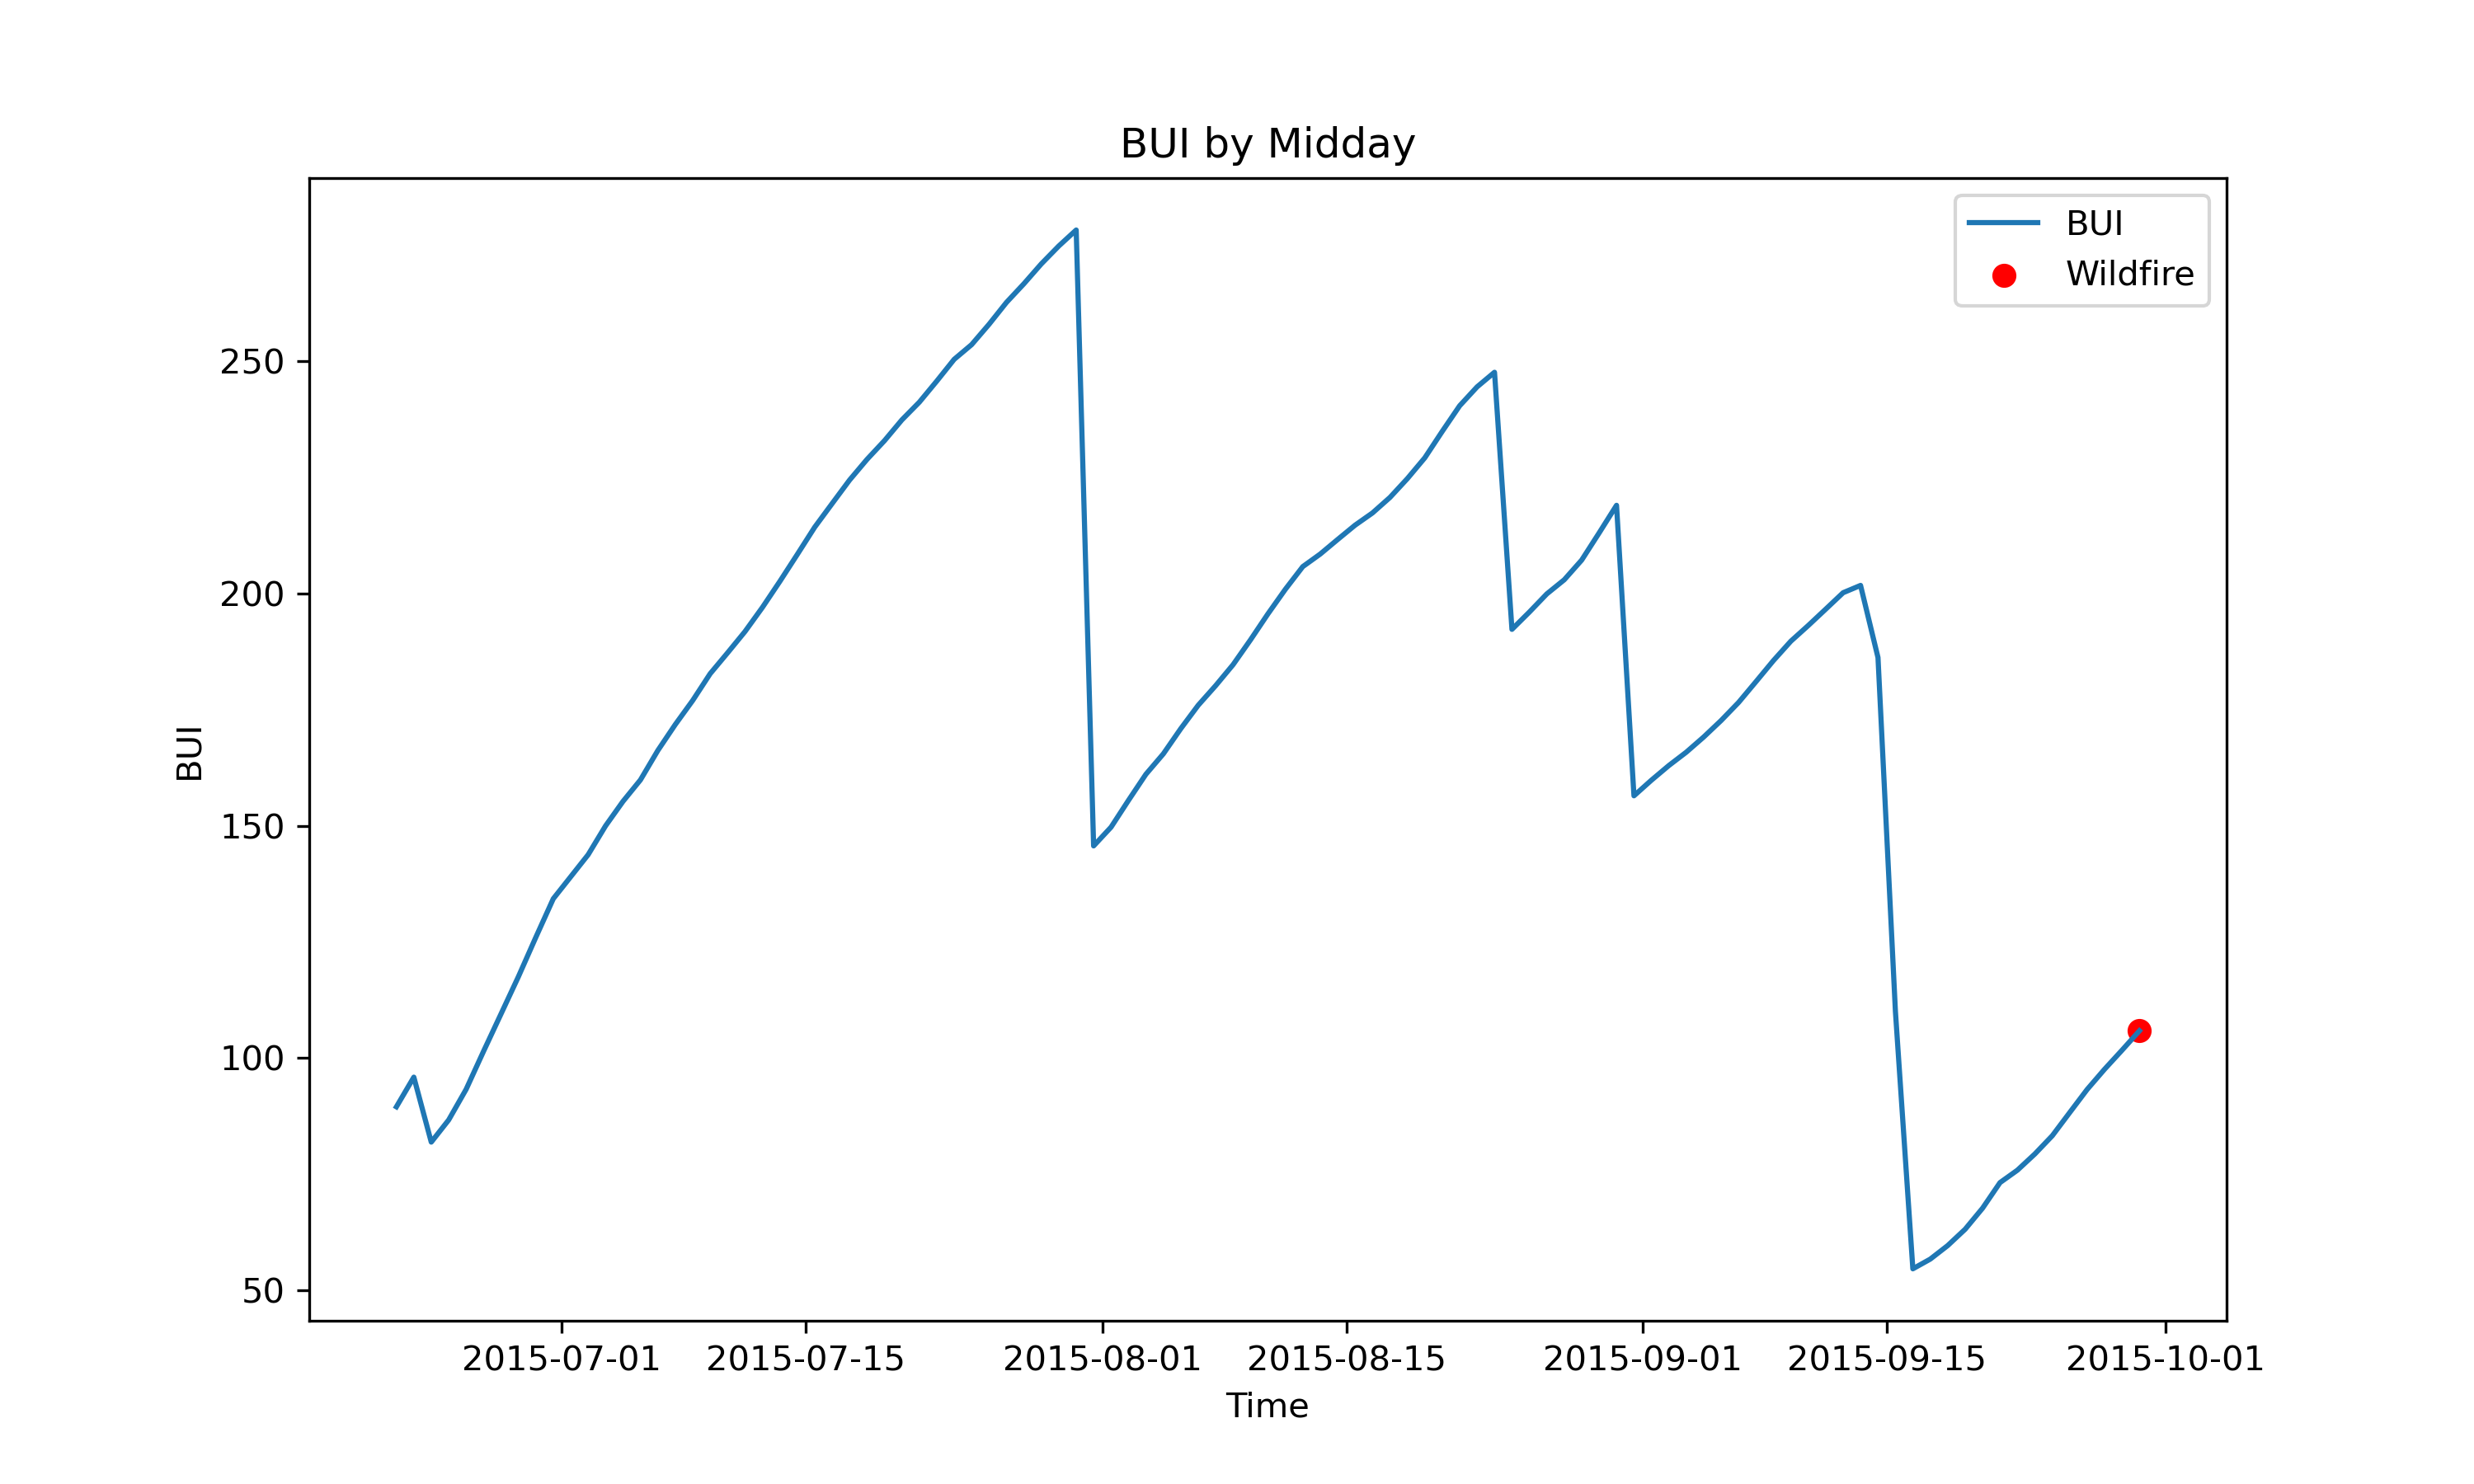
\includegraphics[width=\textwidth]{graphs/2015MesmoSitio/2015CalcBUI12.png}
        \caption{Caption for image 2}
        \label{fig:img2}
    \end{subfigure}
    \label{fig:both_images}
\end{figure}

\FloatBarrier

\section{Comparison of Copernicus and Simulated FWI}
Fogo de 2015
\begin{figure}[h]
\caption{HELLo}
    \centering
    \begin{subfigure}{0.49\textwidth}
        \centering
        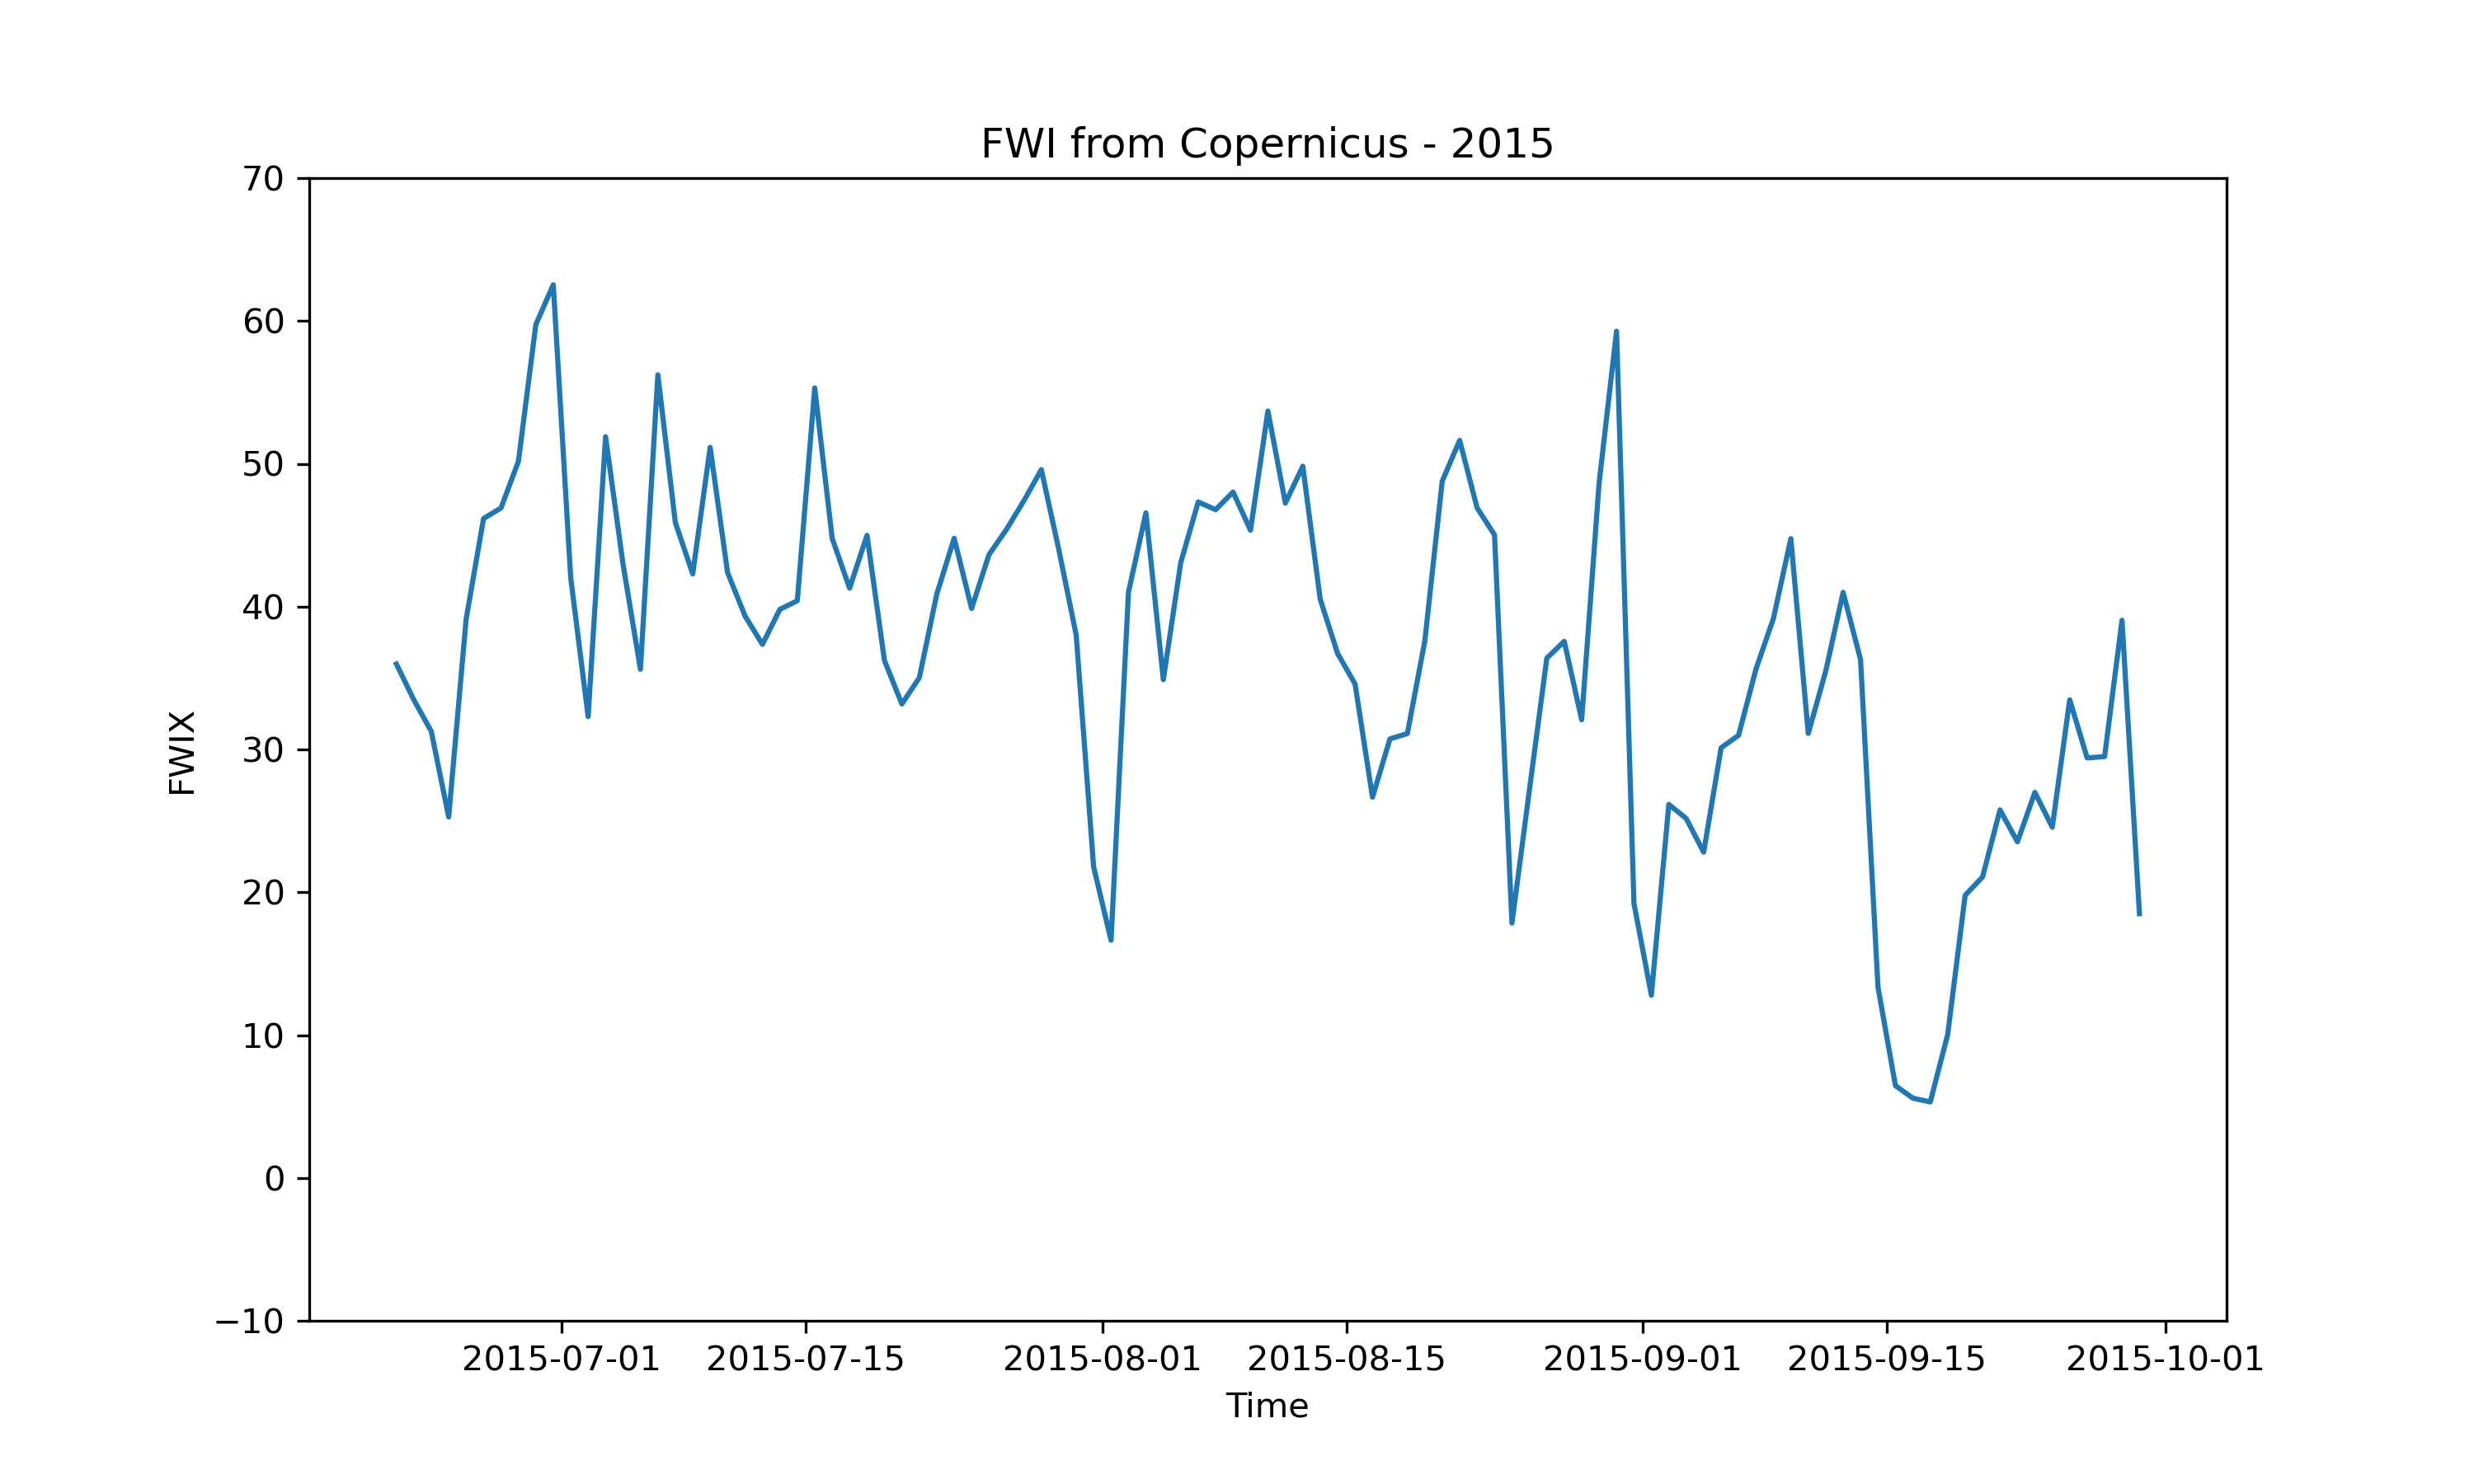
\includegraphics[width=\textwidth]{graphs/2015/2015CopernicusFWI12.png}
        \caption{Caption for image 1}
        \label{fig:img1}
    \end{subfigure}
    \hfill
    \begin{subfigure}{0.49\textwidth}
        \centering
        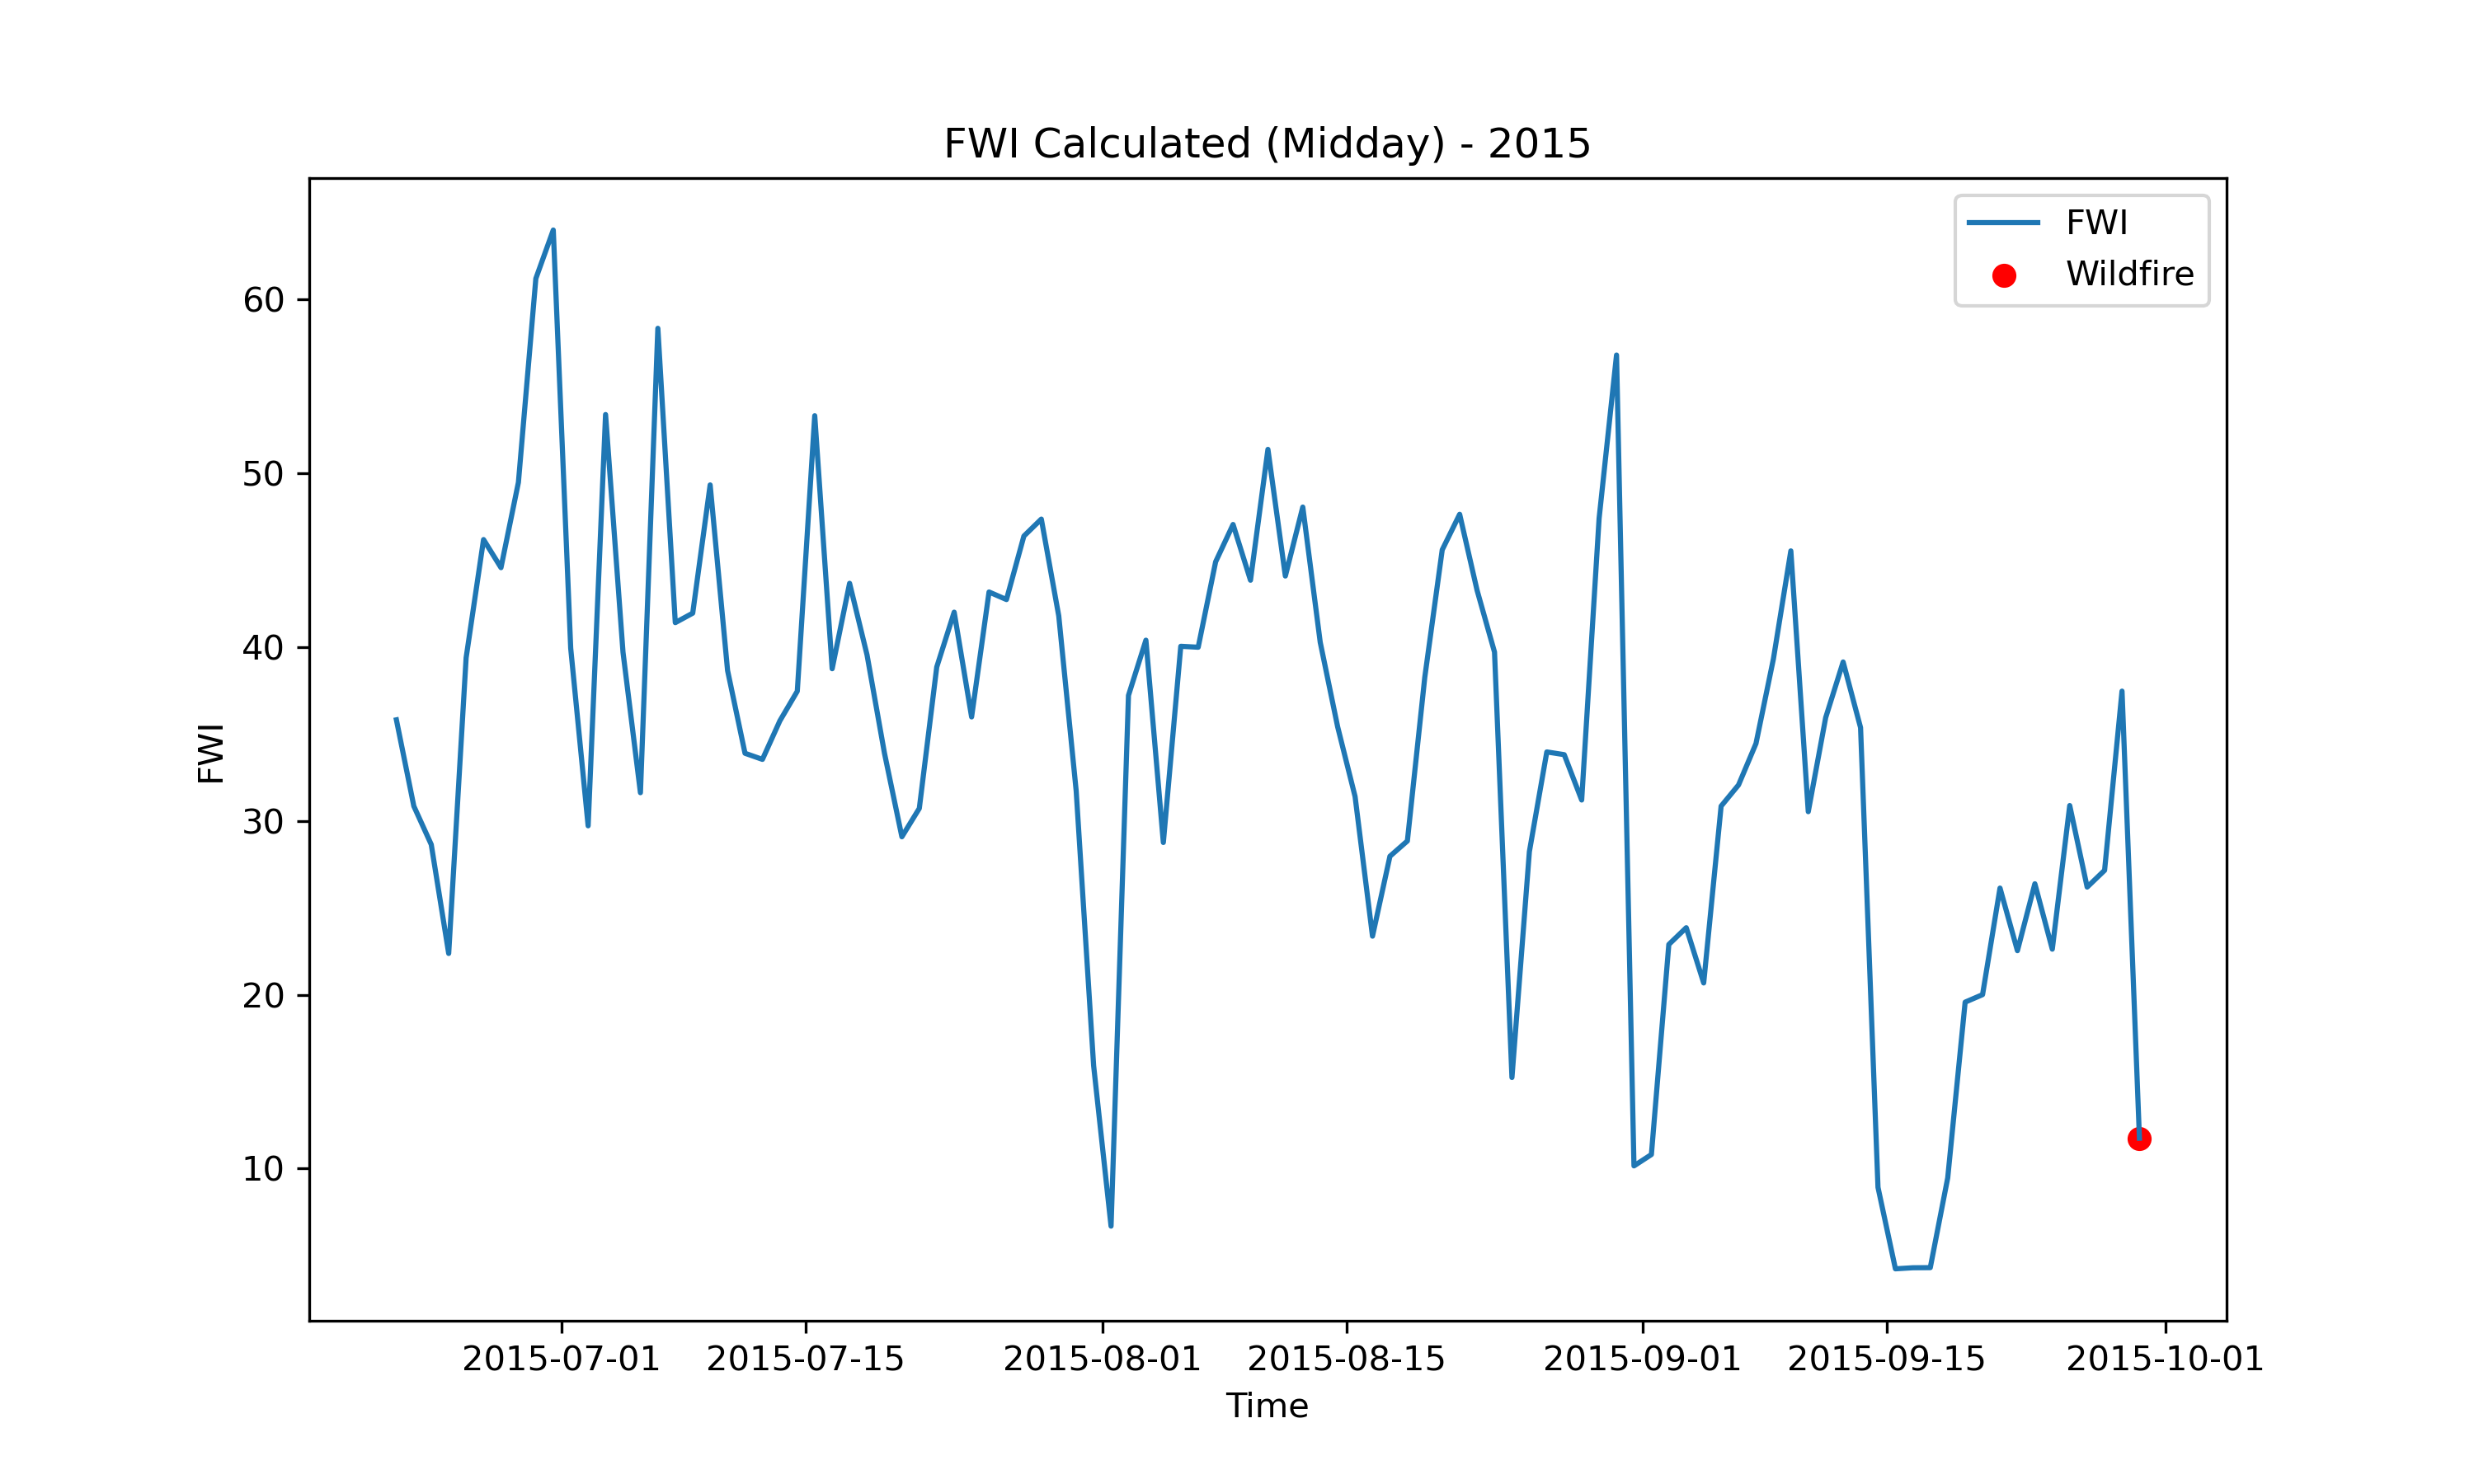
\includegraphics[width=\textwidth]{graphs/2015/2015CalcFWI12.png}
        \caption{Caption for image 2}
        \label{fig:img2}
    \end{subfigure}
    \label{fig:both_images}
\end{figure}

\begin{figure}[h]
\caption{HELLo}
    \centering
    \begin{subfigure}{0.49\textwidth}
        \centering
        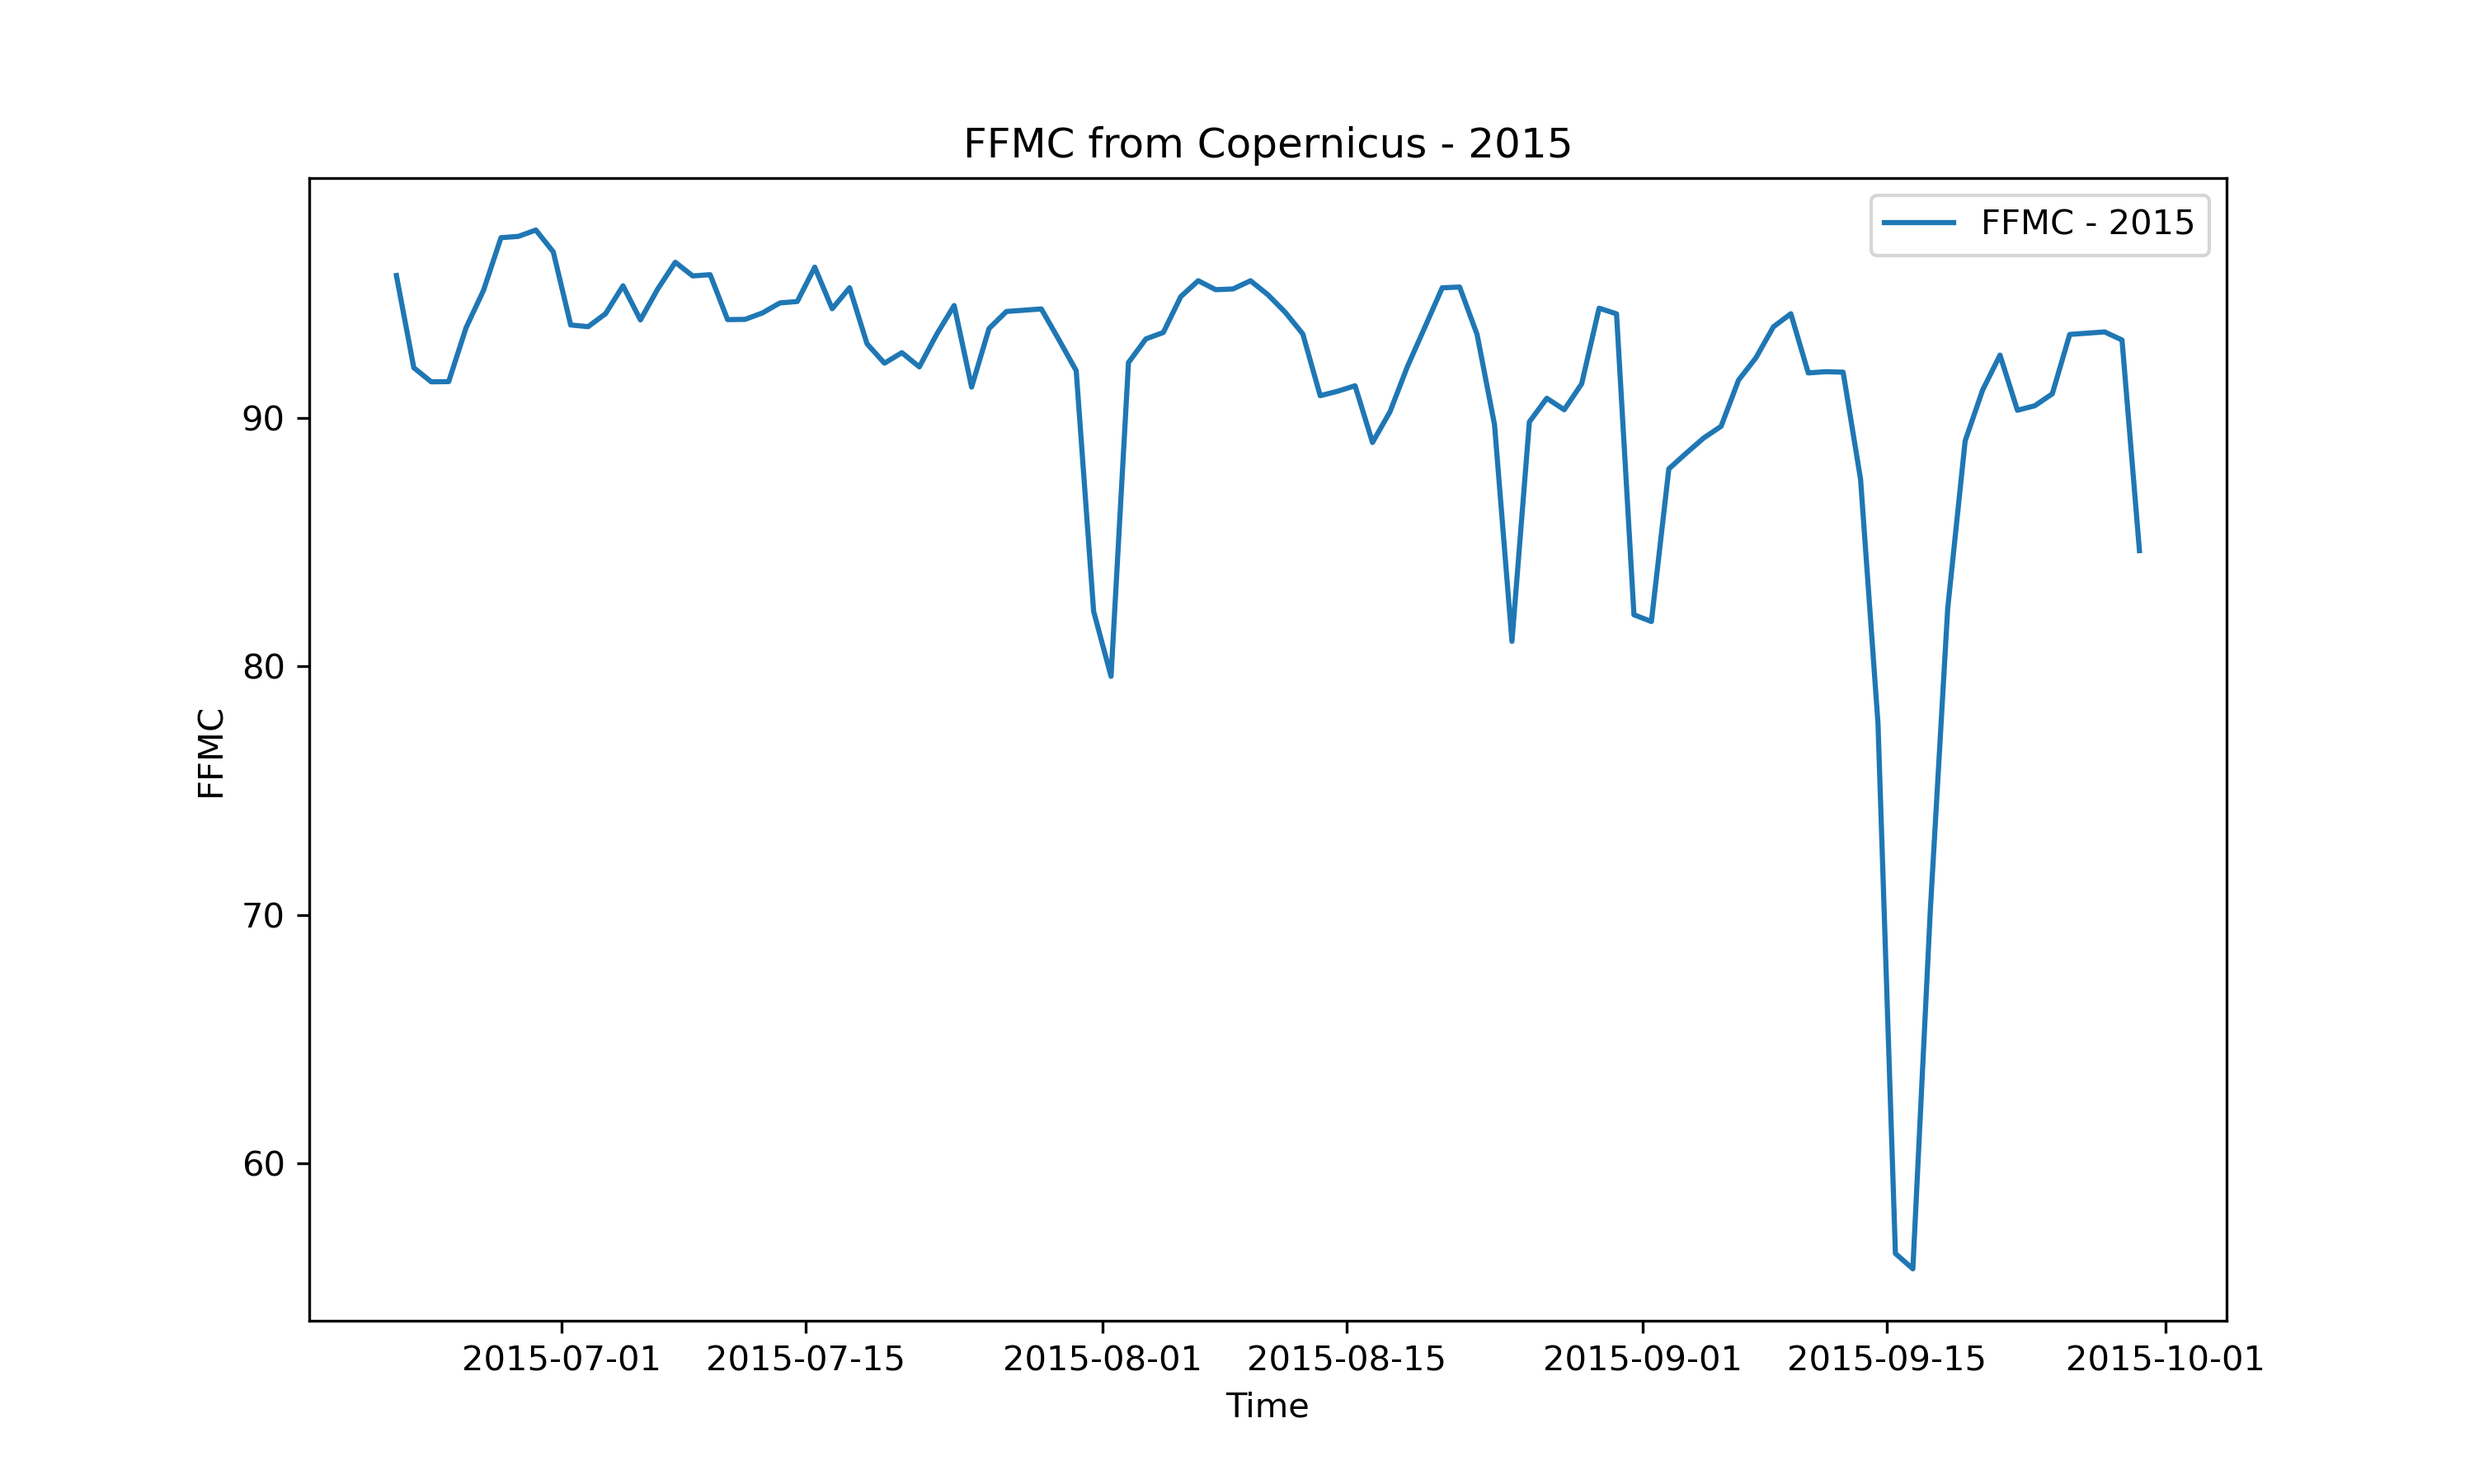
\includegraphics[width=\textwidth]{graphs/2015/2015CopernicusFFMC12.png}
        \caption{Caption for image 1}
        \label{fig:img1}
    \end{subfigure}
    \hfill
    \begin{subfigure}{0.49\textwidth}
        \centering
        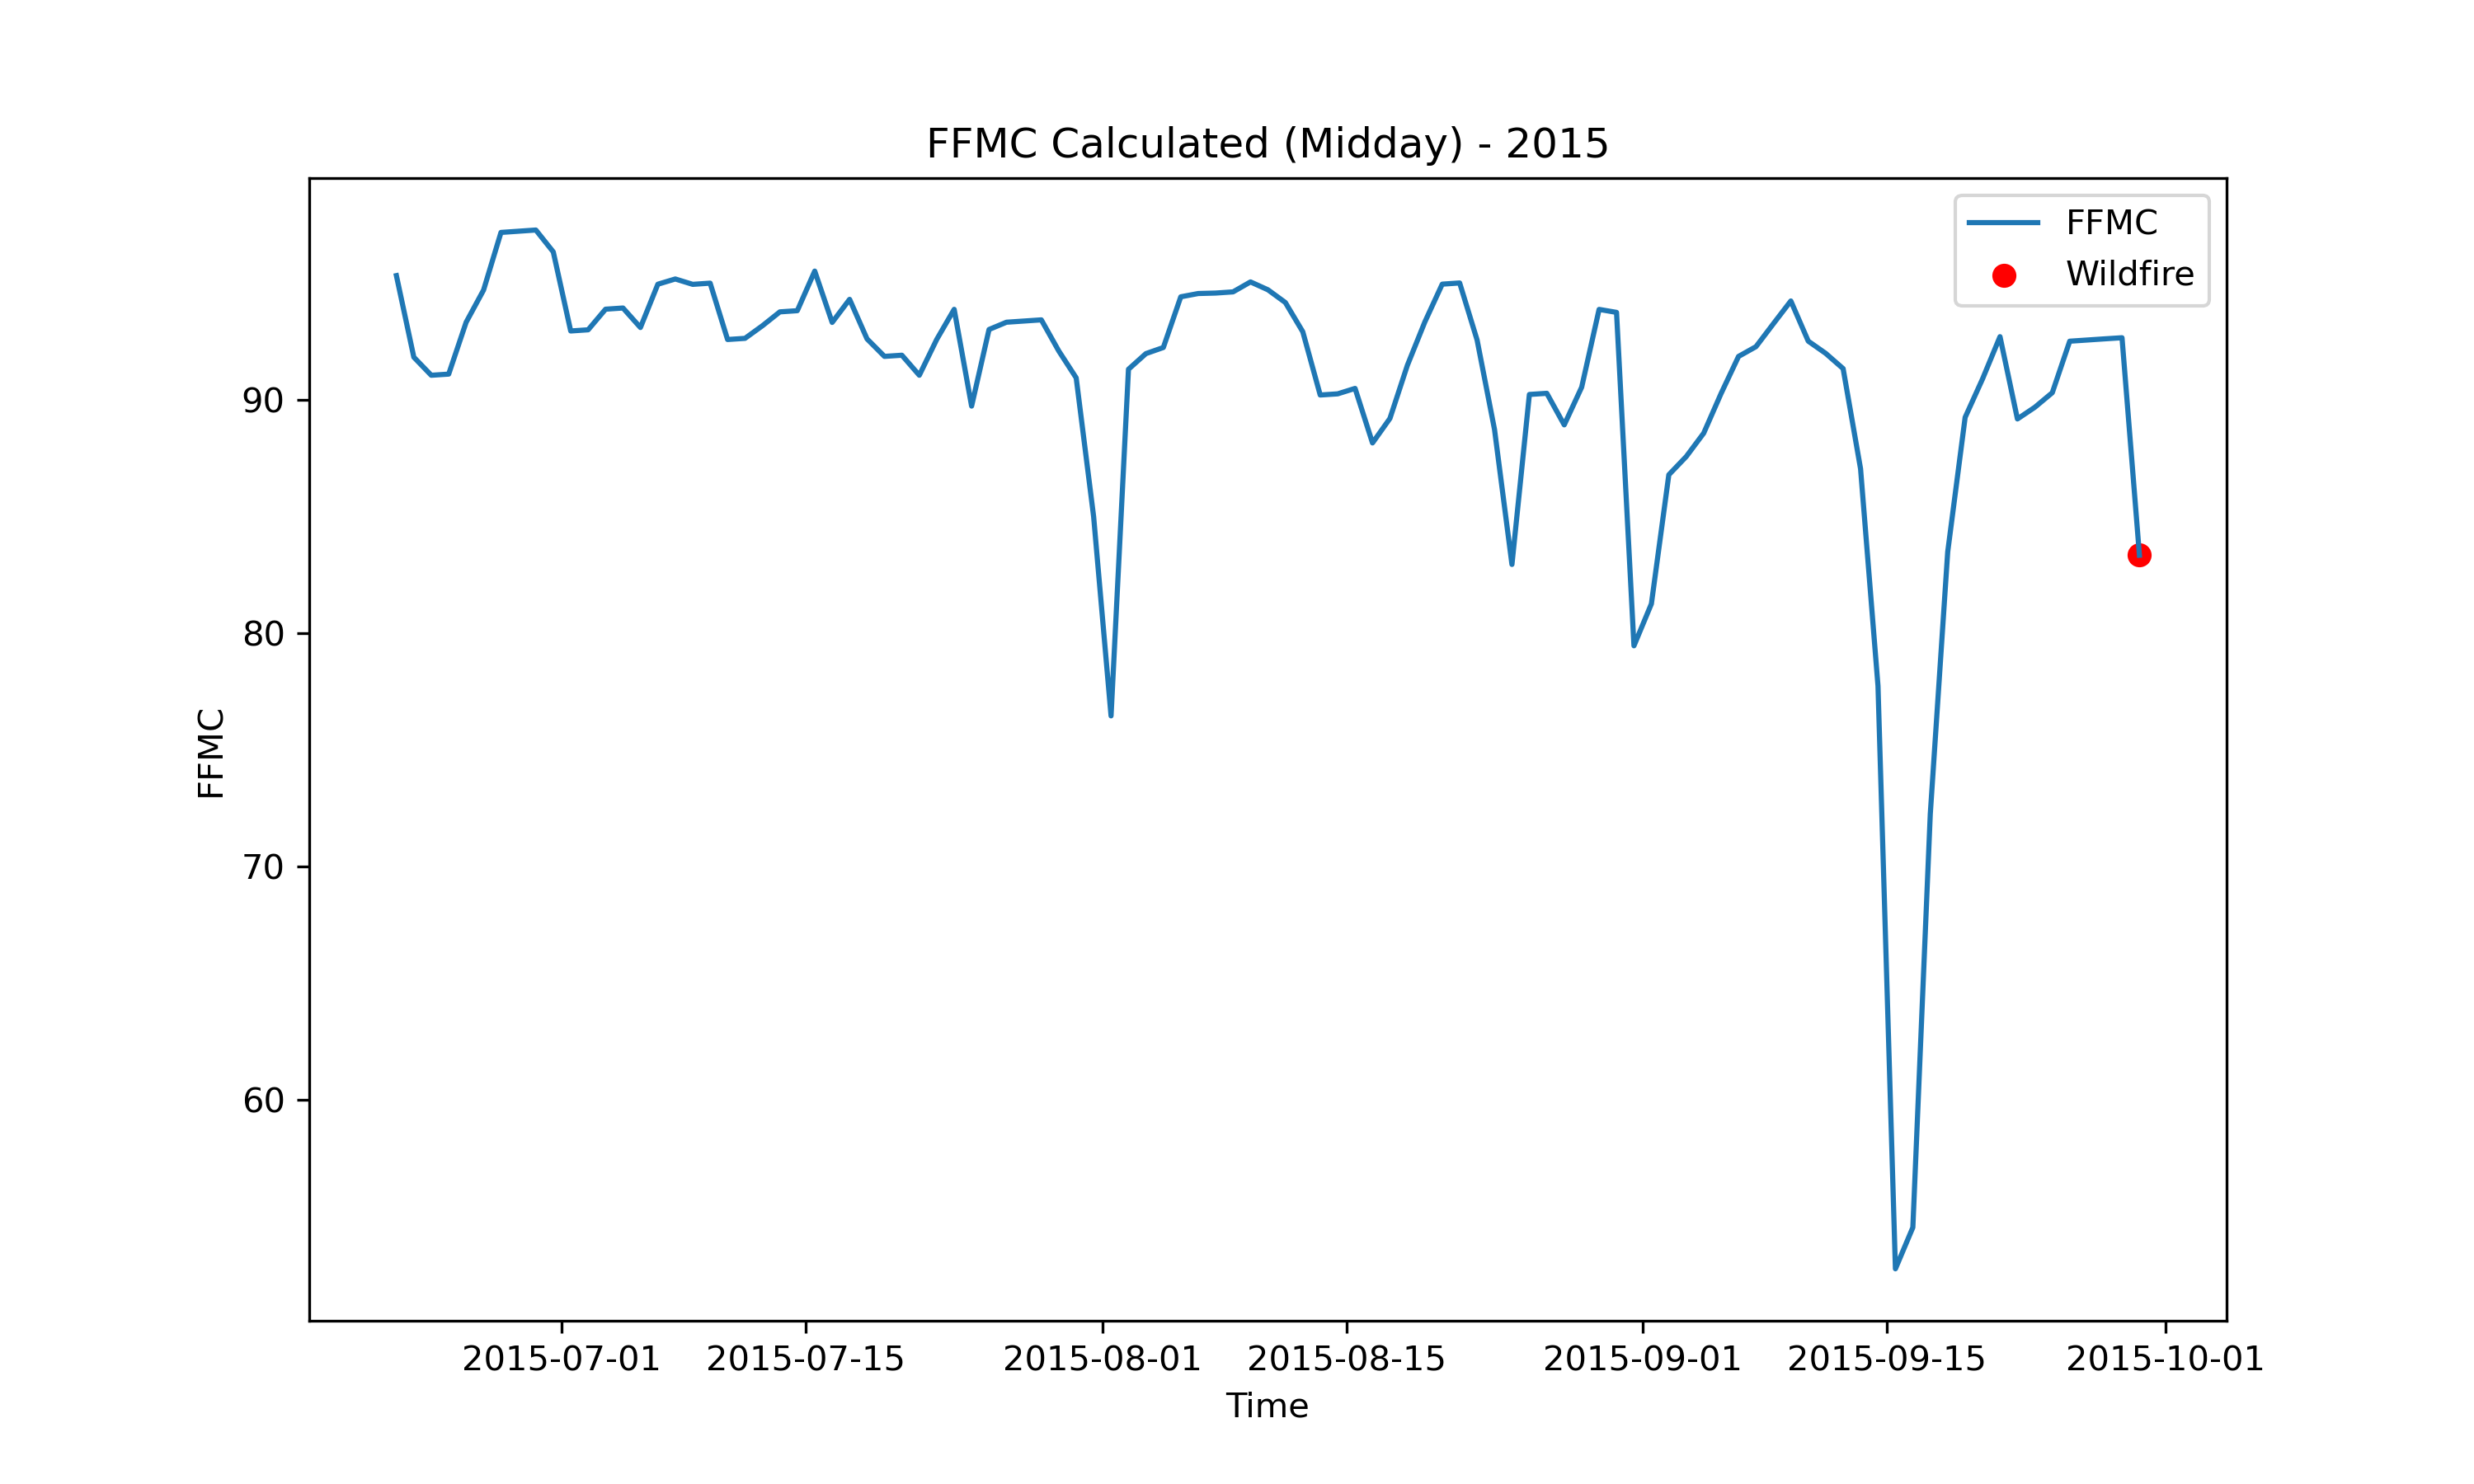
\includegraphics[width=\textwidth]{graphs/2015/2015CalcFFMC12.png}
        \caption{Caption for image 2}
        \label{fig:img2}
    \end{subfigure}
    \label{fig:both_images}
\end{figure}

\begin{figure}[h]
\caption{HELLo}
    \centering
    \begin{subfigure}{0.49\textwidth}
        \centering
        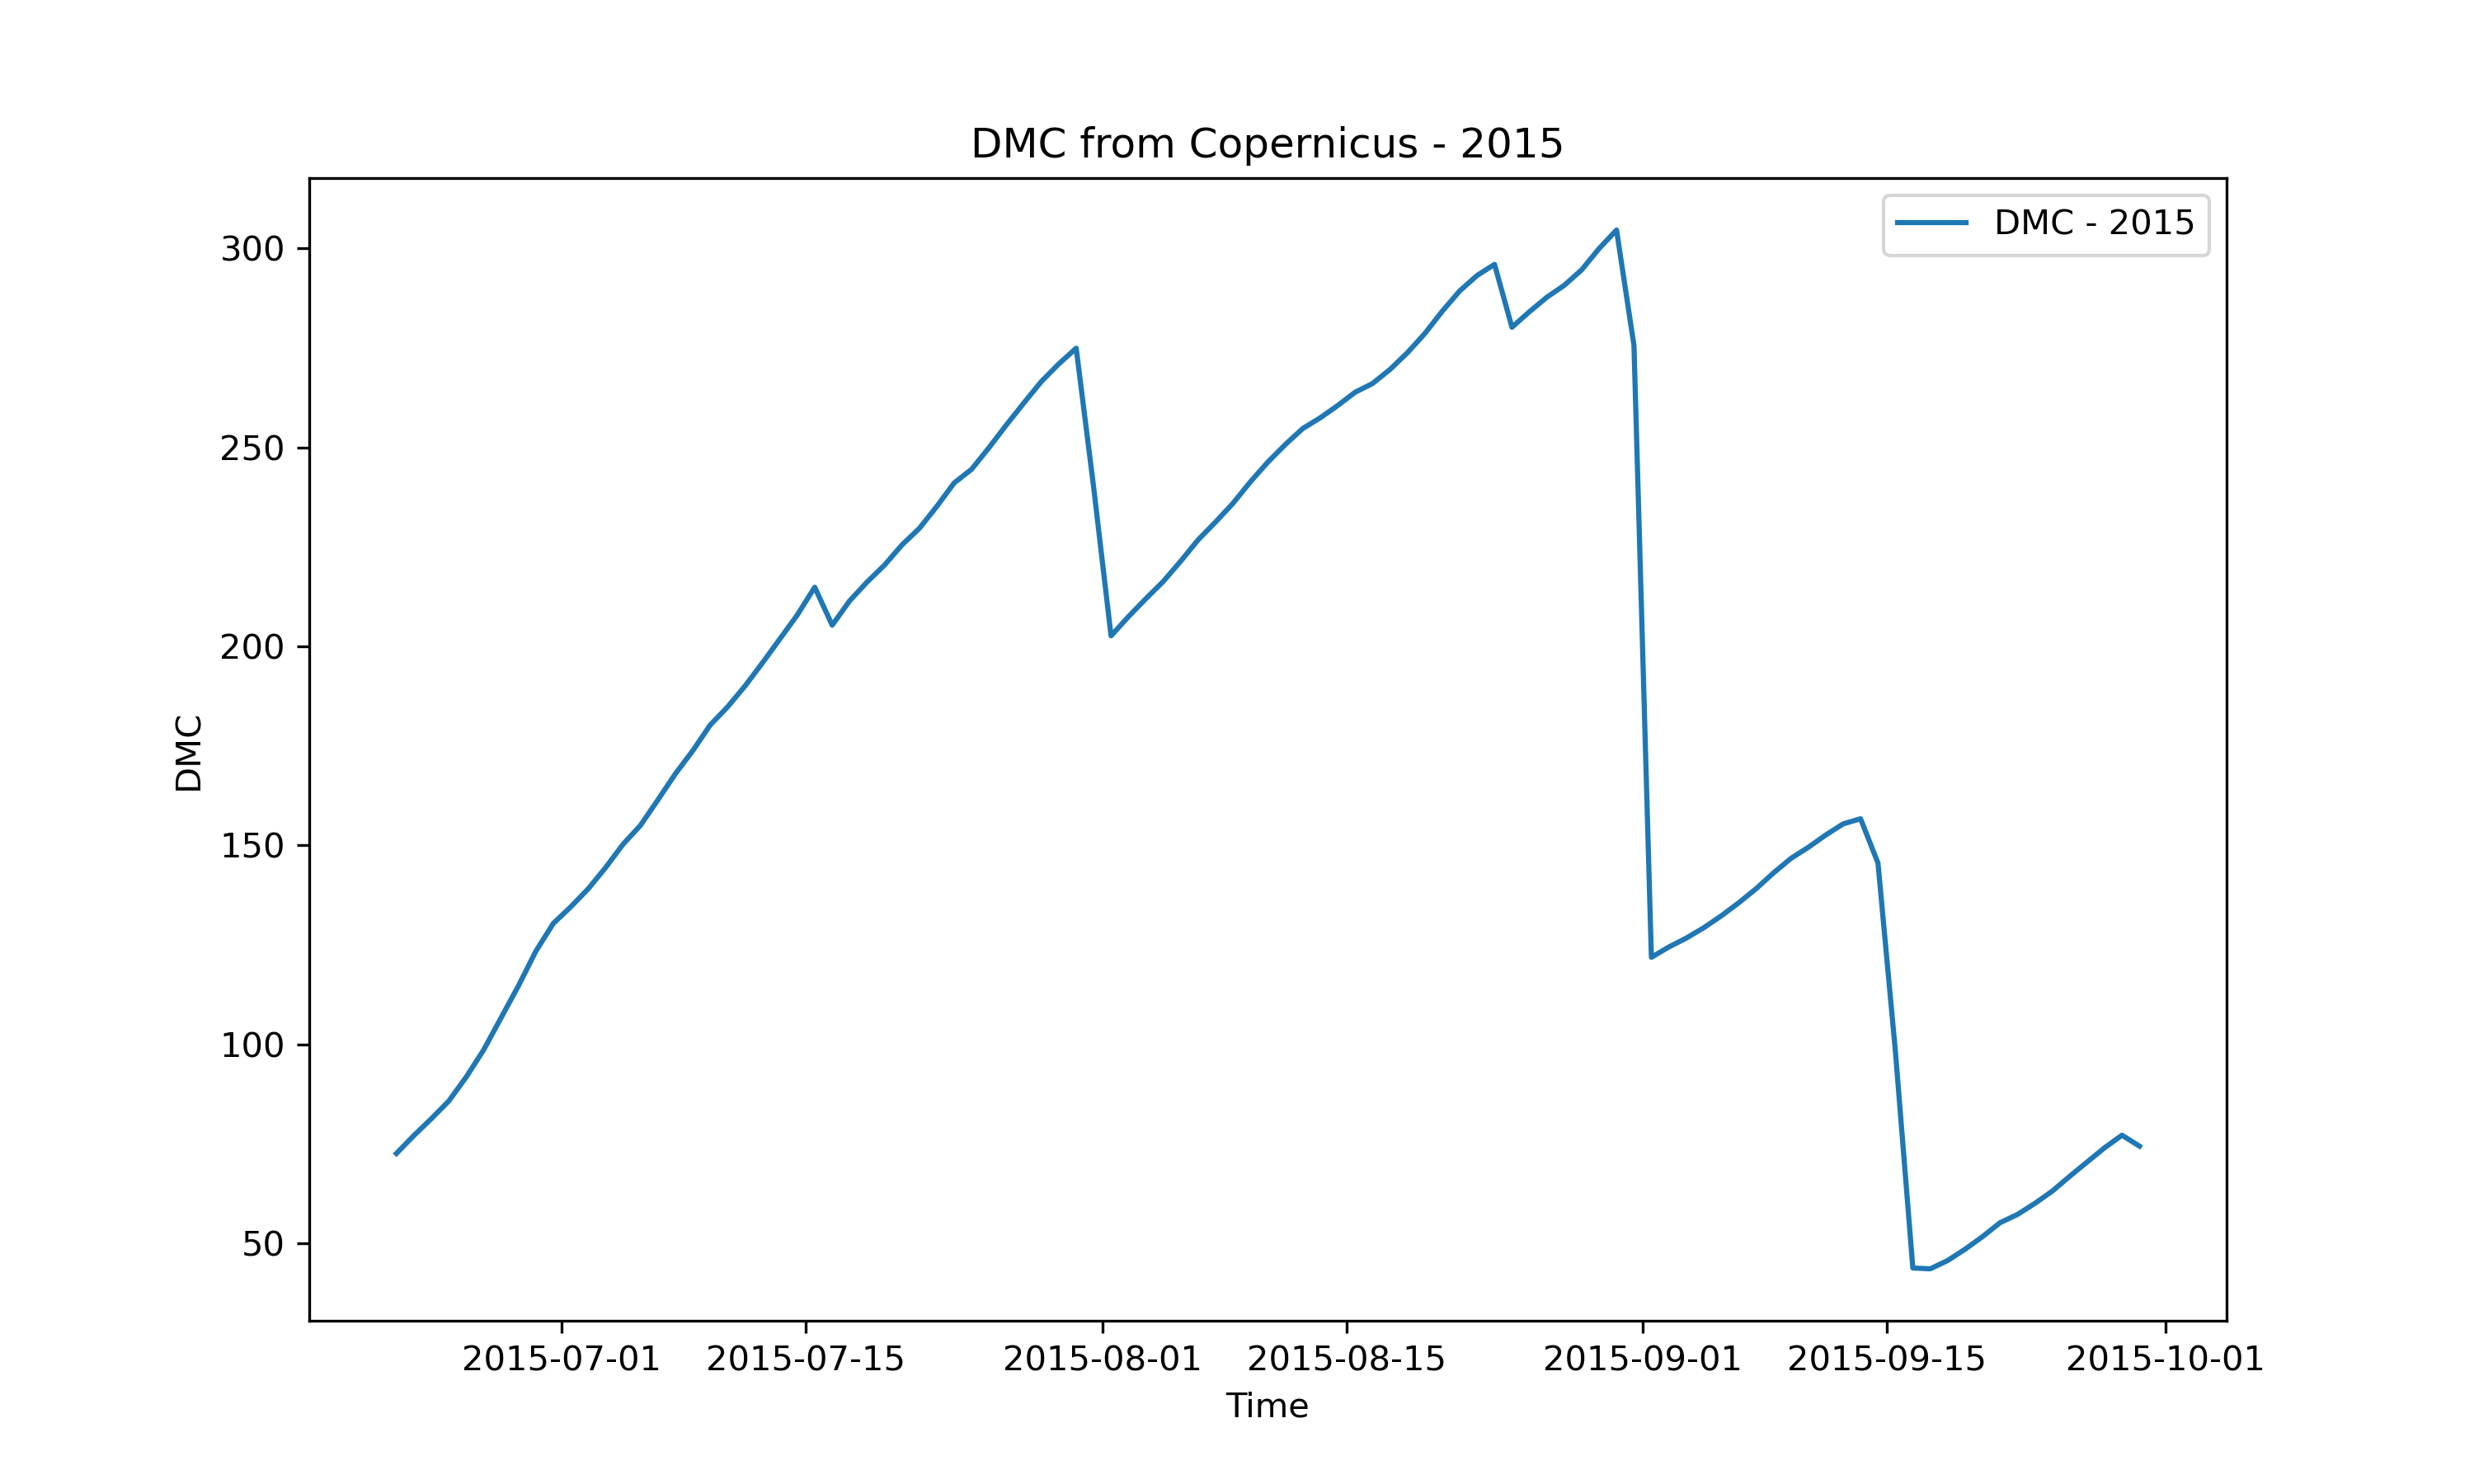
\includegraphics[width=\textwidth]{graphs/2015/2015CopernicusDMC12.png}
        \caption{Caption for image 1}
        \label{fig:img1}
    \end{subfigure}
    \hfill
    \begin{subfigure}{0.49\textwidth}
        \centering
        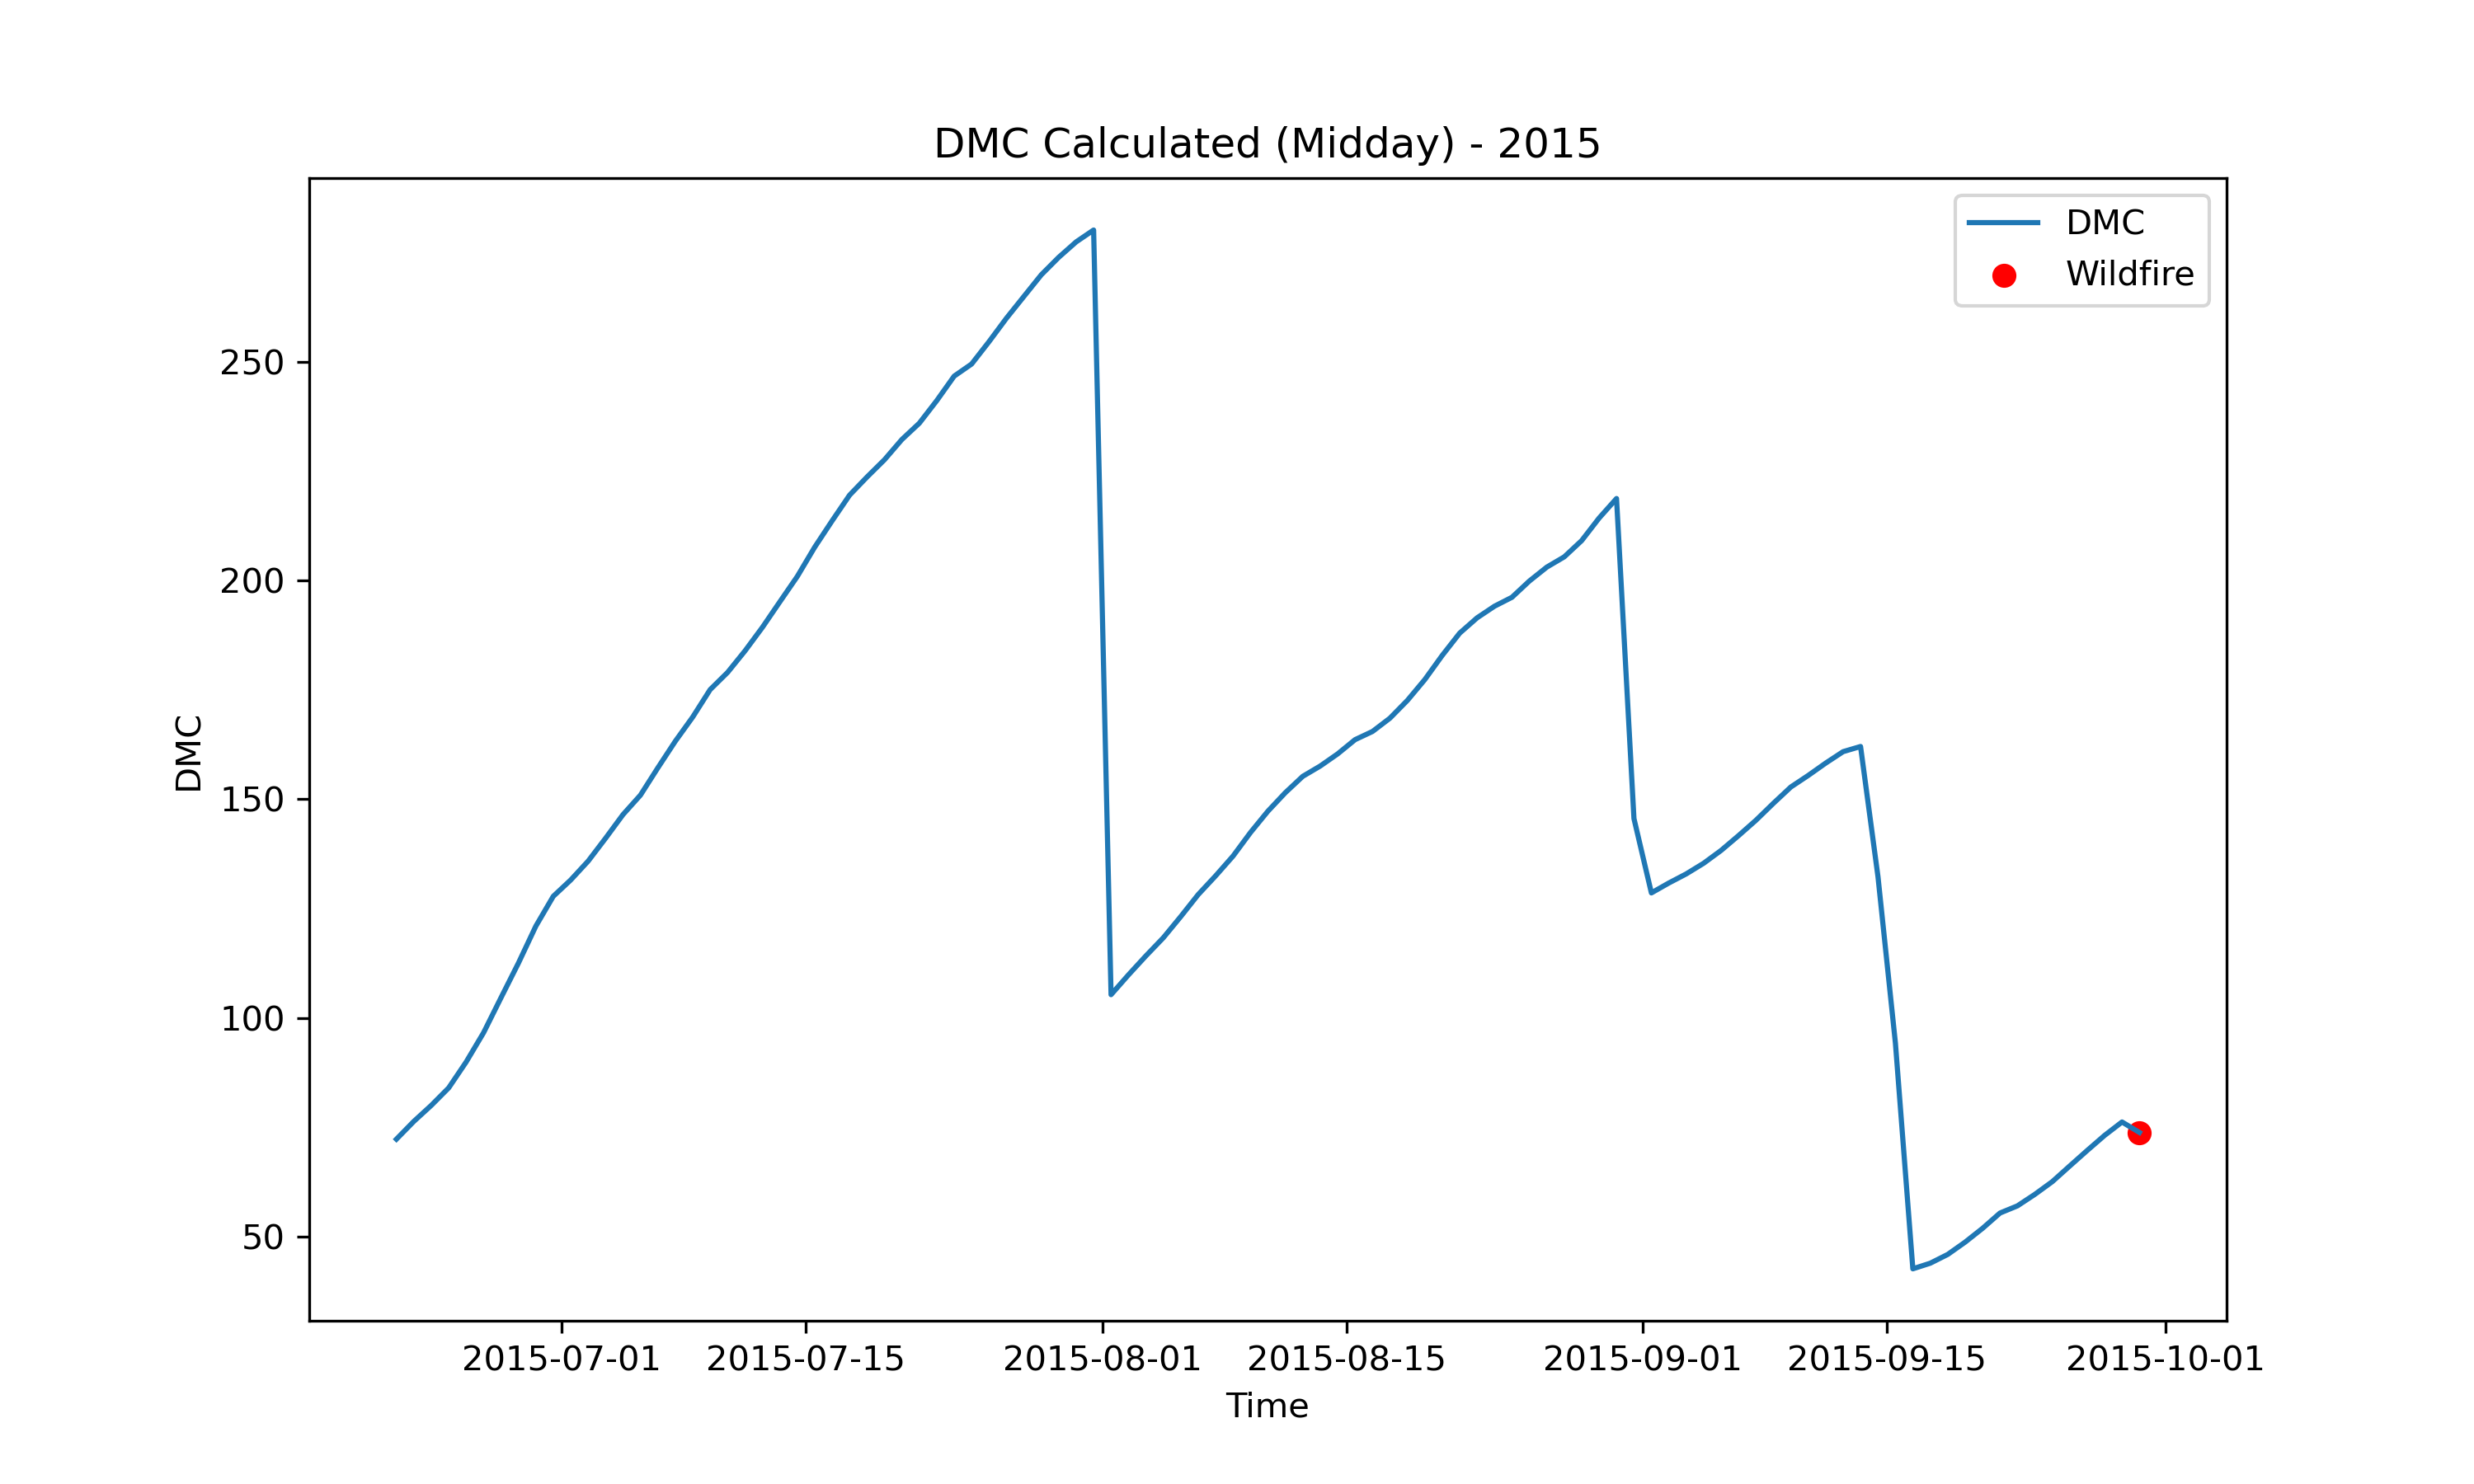
\includegraphics[width=\textwidth]{graphs/2015/2015CalcDMC12.png}
        \caption{Caption for image 2}
        \label{fig:img2}
    \end{subfigure}
    \label{fig:both_images}
\end{figure}

\begin{figure}[h]
\caption{HELLo}
    \centering
    \begin{subfigure}{0.49\textwidth}
        \centering
        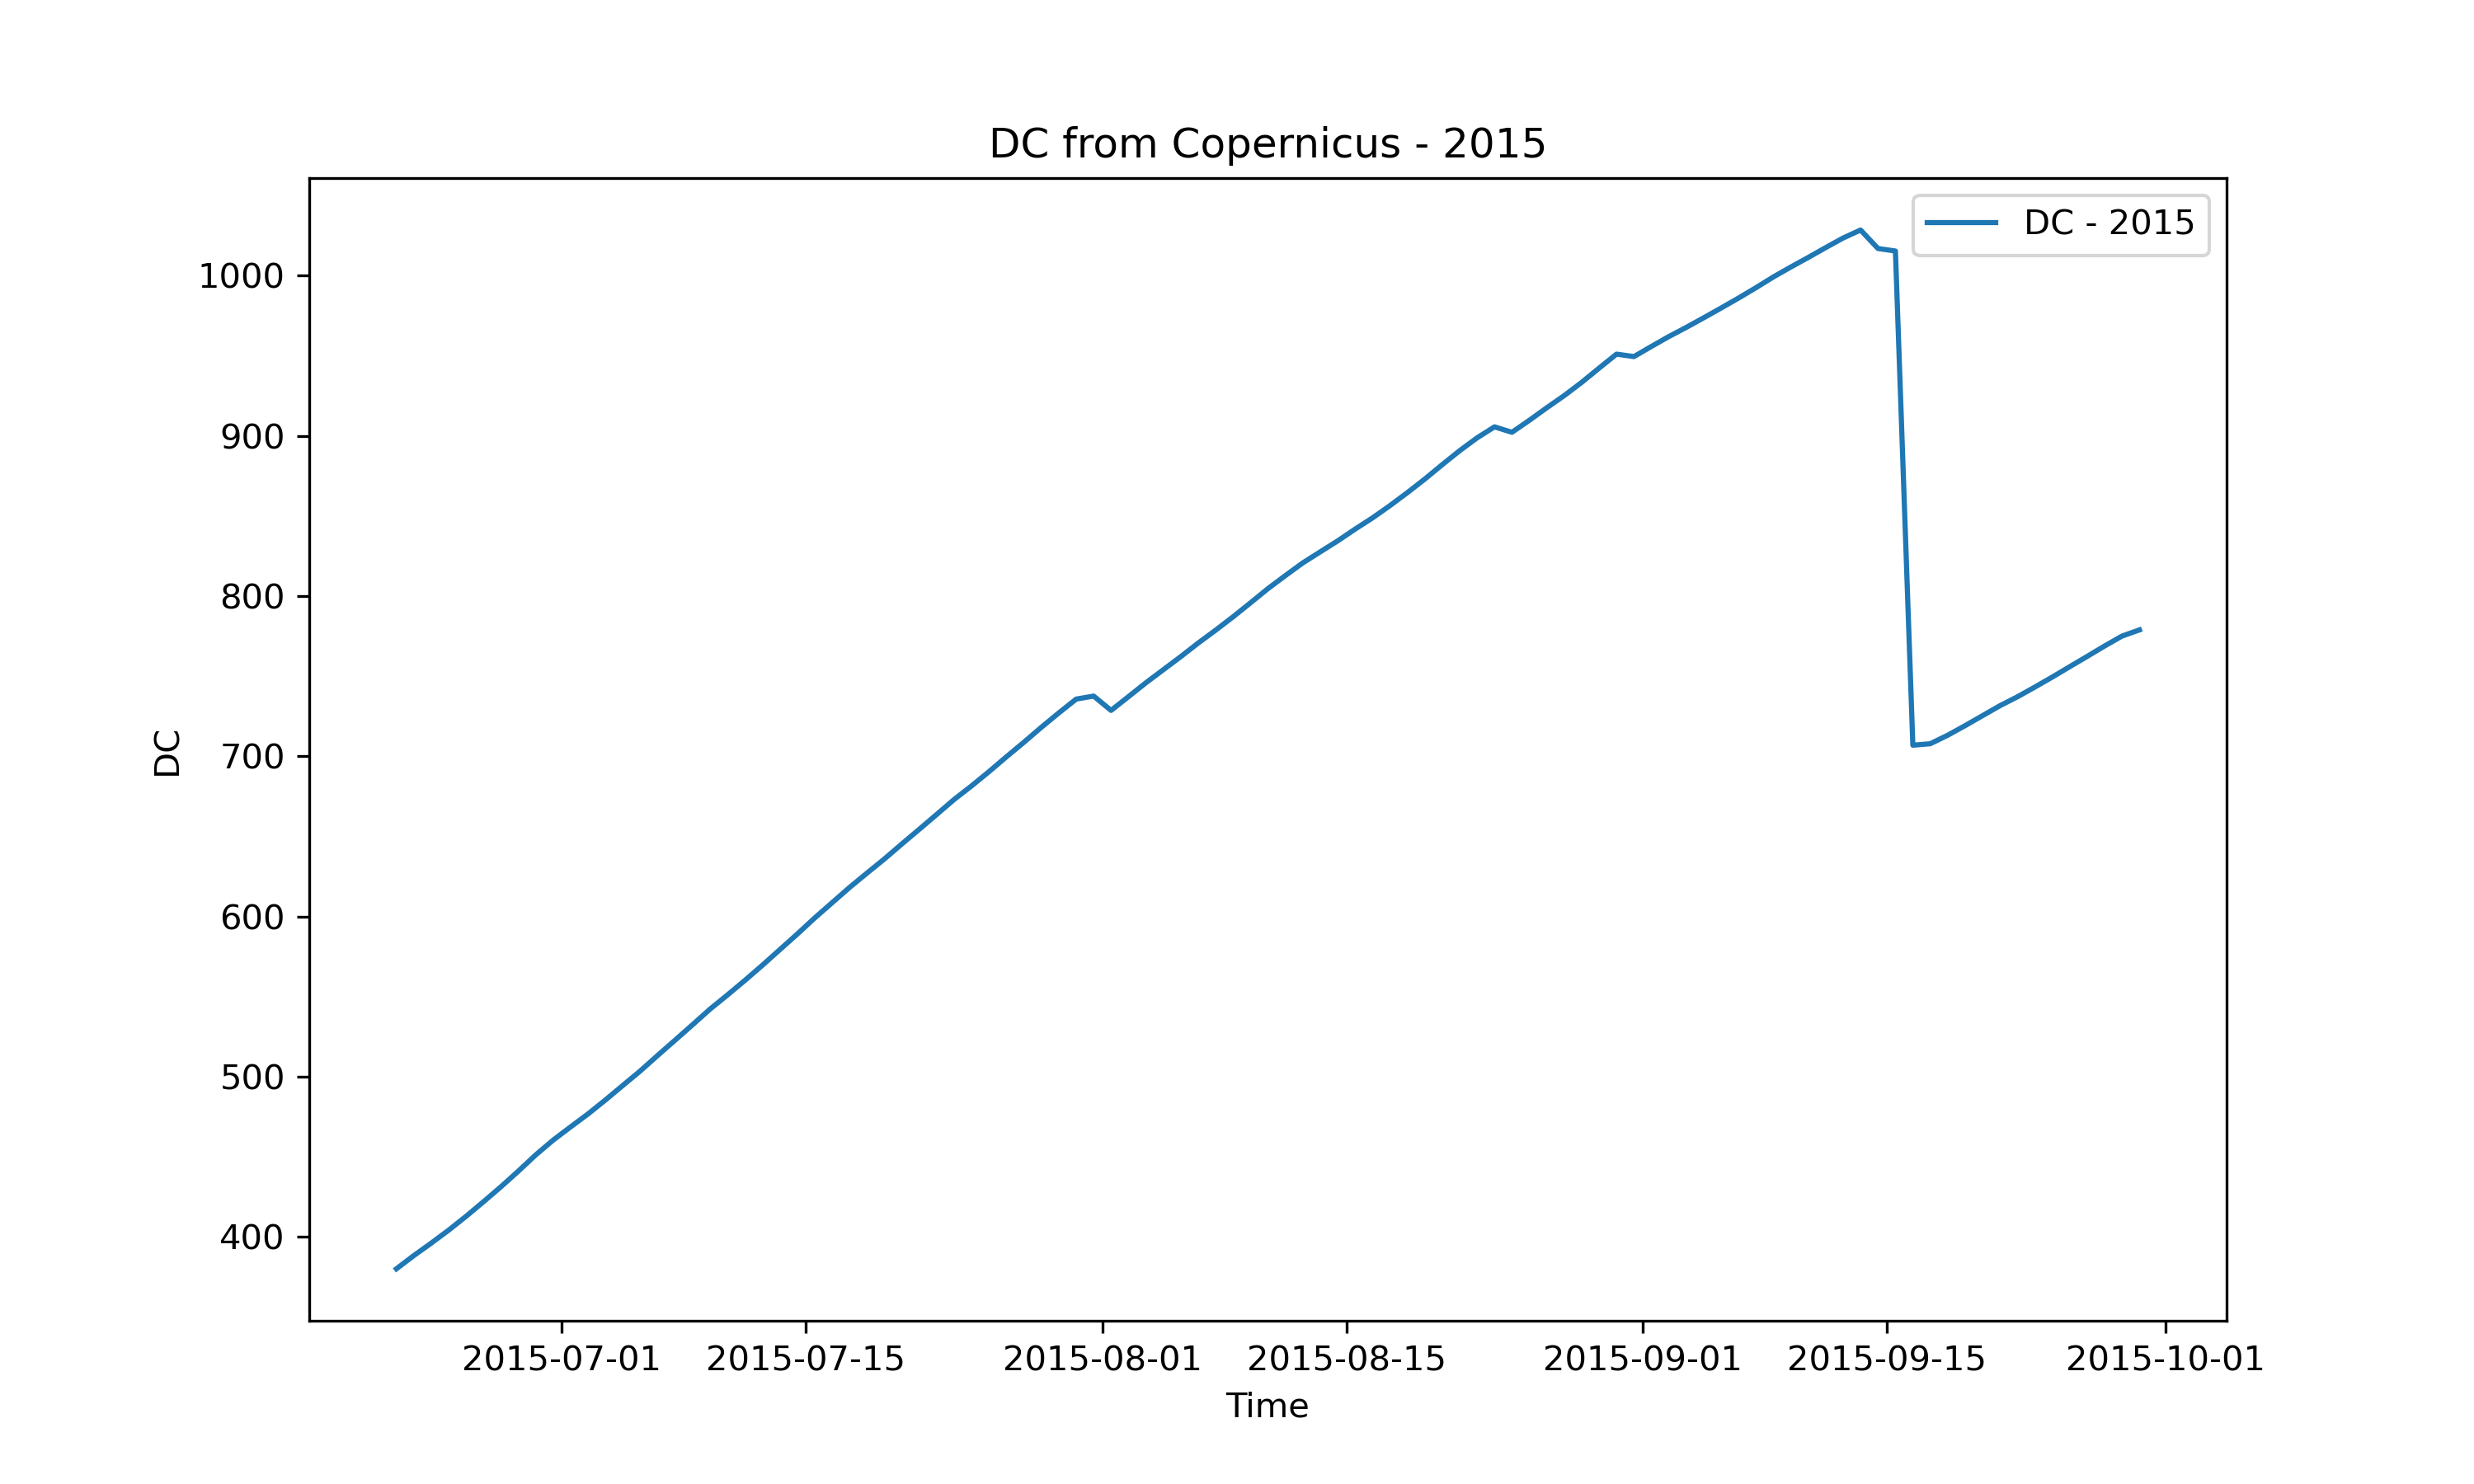
\includegraphics[width=\textwidth]{graphs/2015/2015CopernicusDC12.png}
        \caption{Caption for image 1}
        \label{fig:img1}
    \end{subfigure}
    \hfill
    \begin{subfigure}{0.49\textwidth}
        \centering
        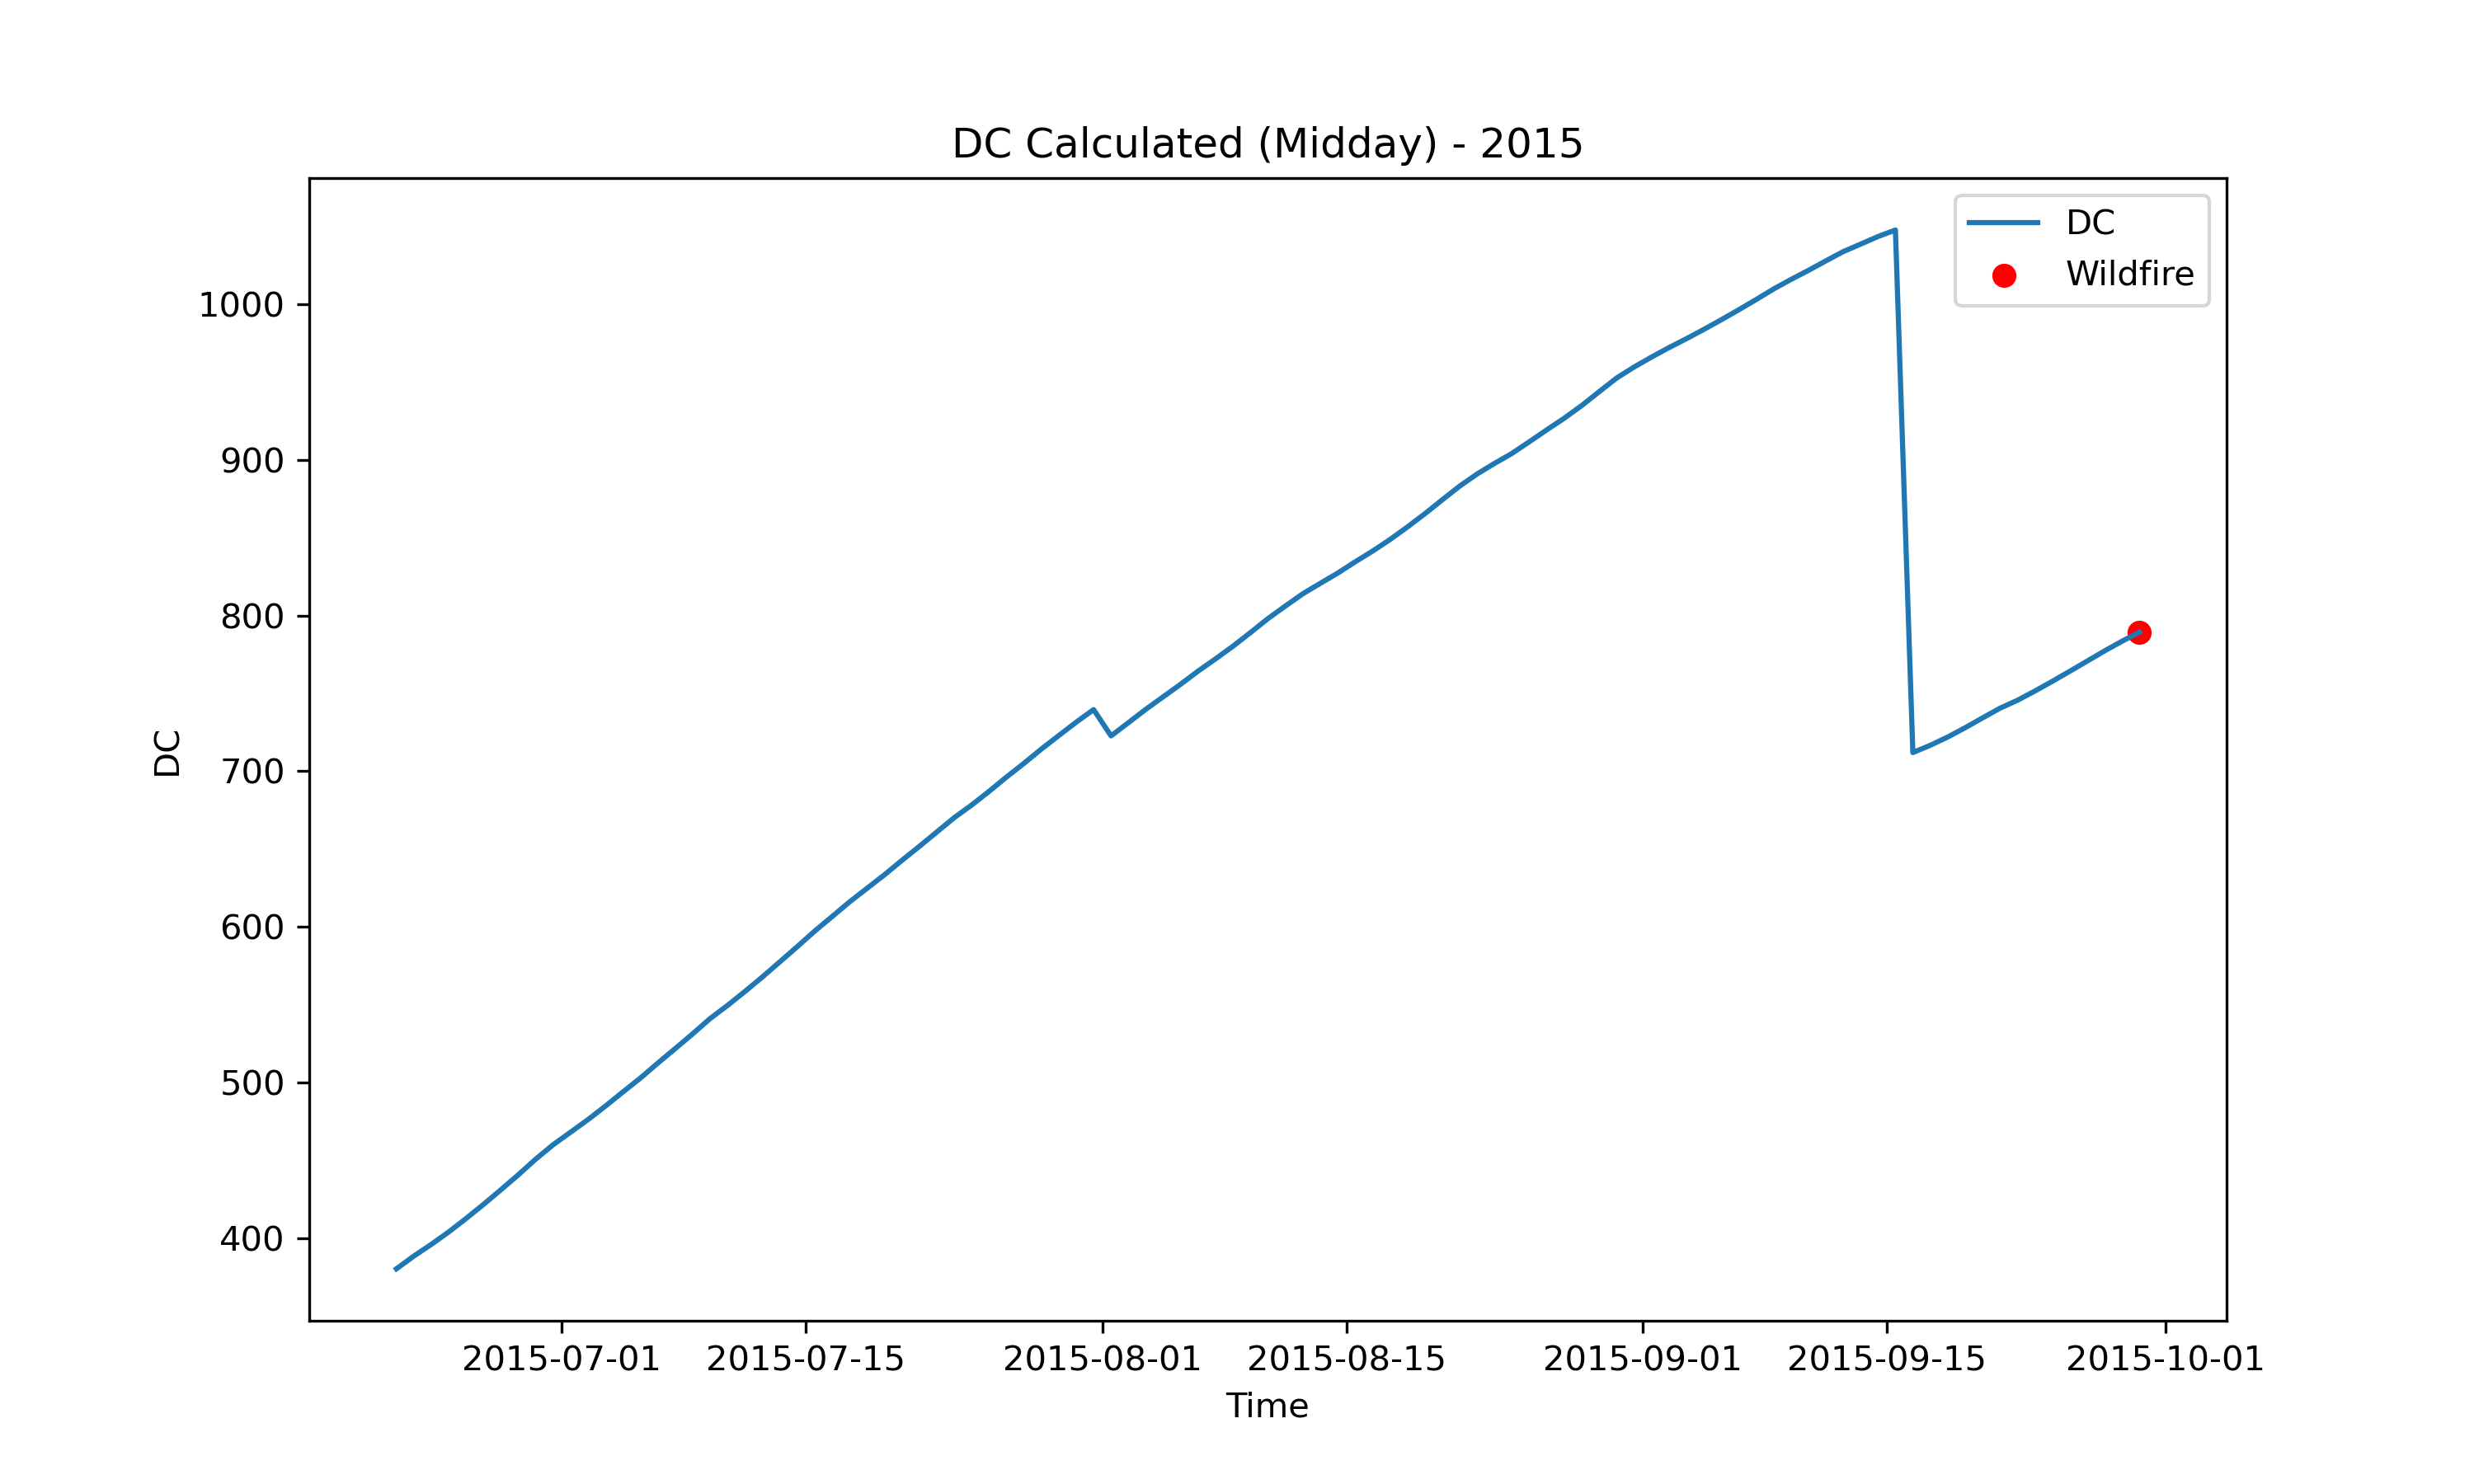
\includegraphics[width=\textwidth]{graphs/2015/2015CalcDC12.png}
        \caption{Caption for image 2}
        \label{fig:img2}
    \end{subfigure}
    \label{fig:both_images}
\end{figure}

\begin{figure}[h]
	\caption{HELLo}
	\centering
	\begin{subfigure}{0.49\textwidth}
		\centering
		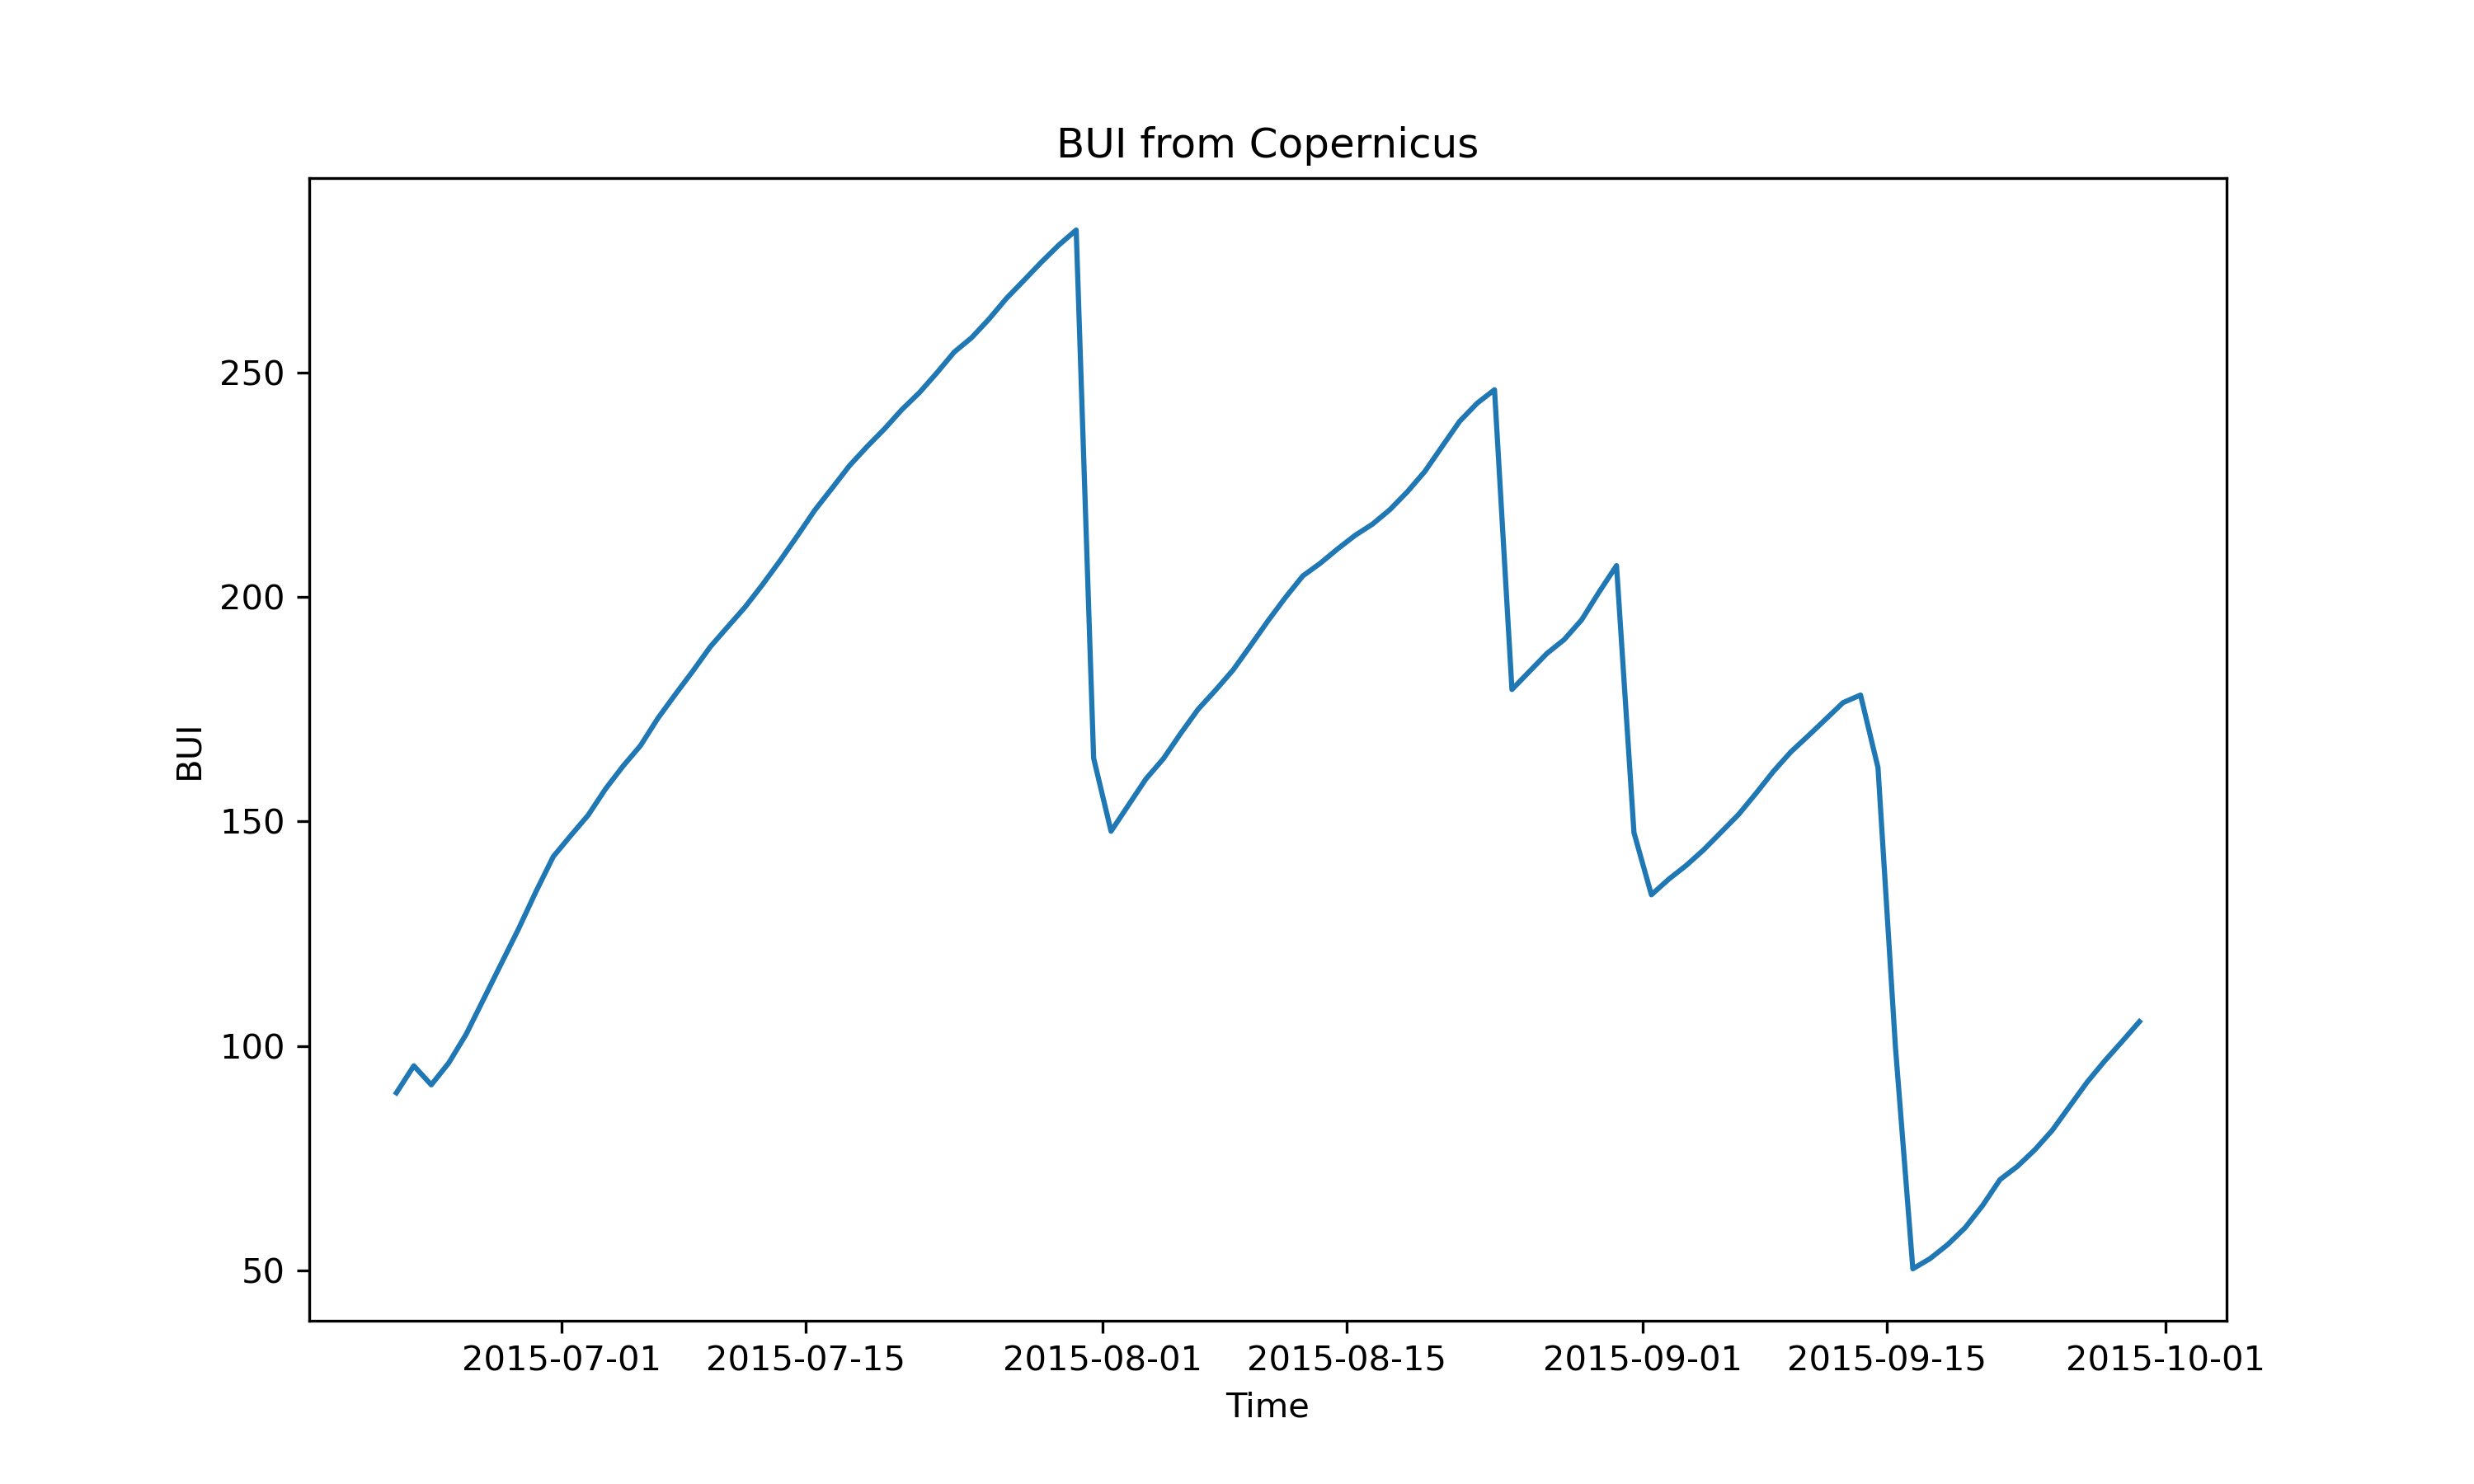
\includegraphics[width=\textwidth]{graphs/2015/2015CopernicusISI12.png}
		\caption{Caption for image 1}
		\label{fig:img1}
	\end{subfigure}
	\hfill
	\begin{subfigure}{0.49\textwidth}
		\centering
		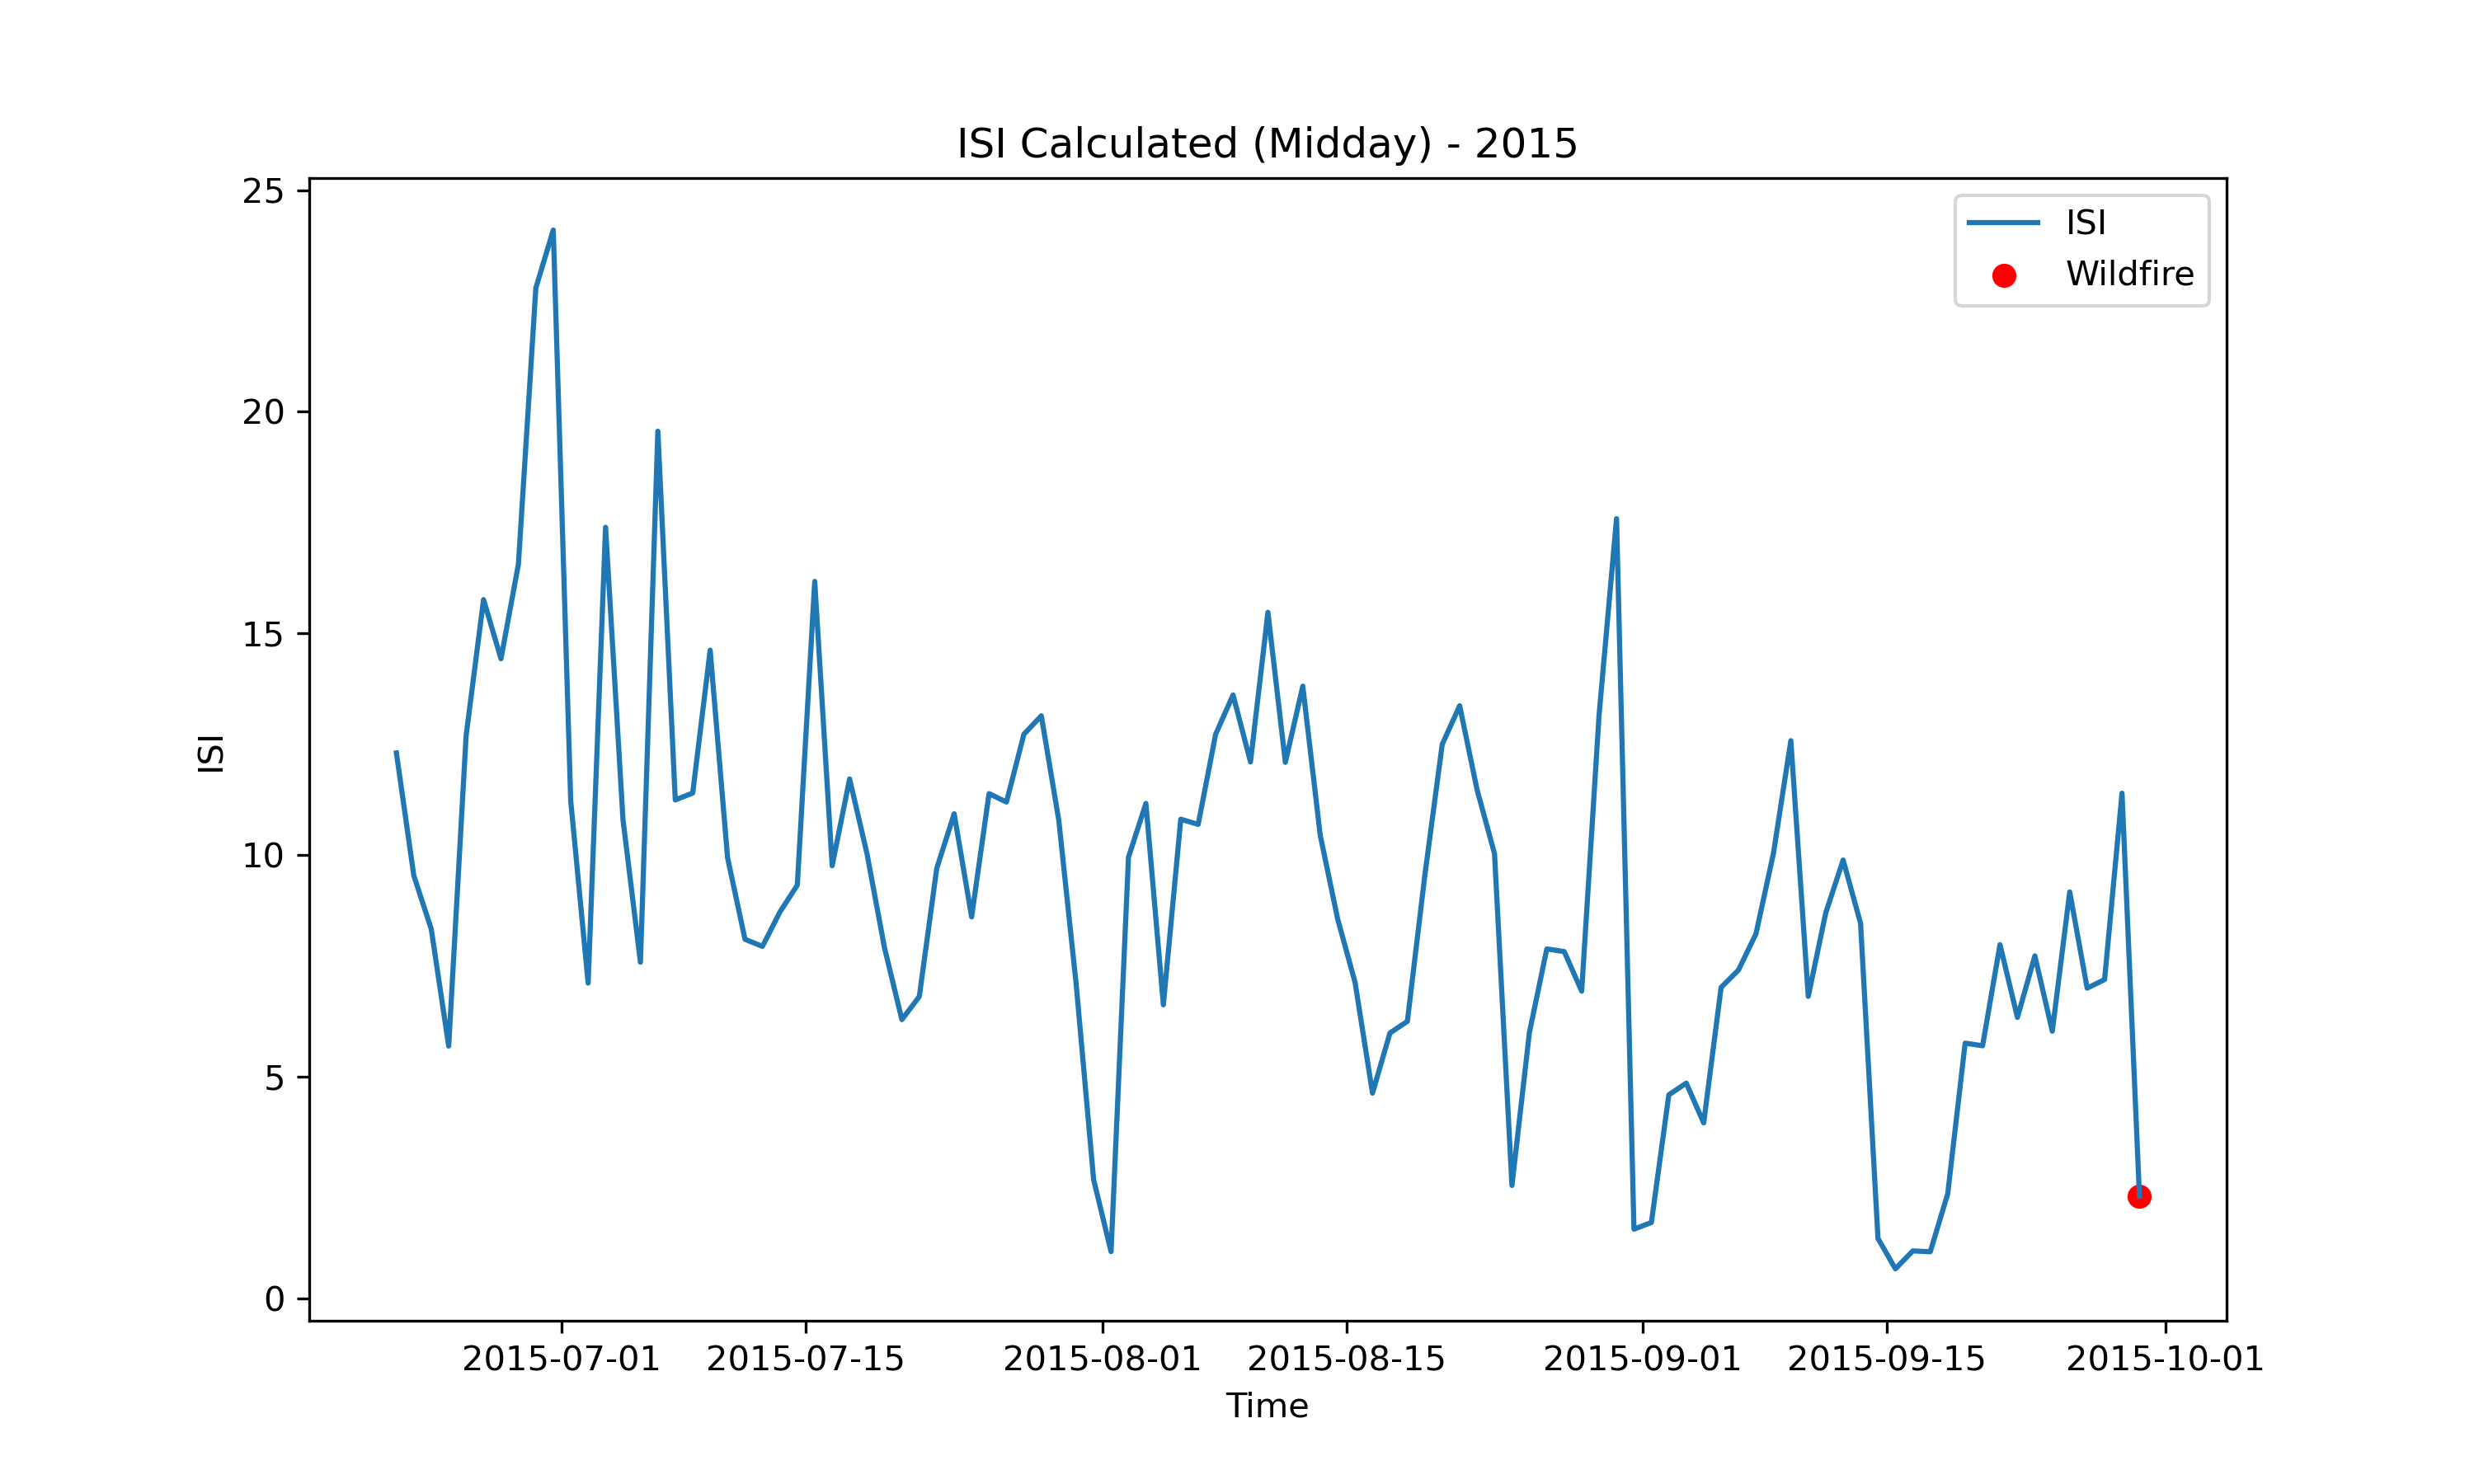
\includegraphics[width=\textwidth]{graphs/2015/2015CalcISI12.png}
		\caption{Caption for image 2}
		\label{fig:img2}
	\end{subfigure}
	\label{fig:both_images}
\end{figure}

\begin{figure}[h]
	\caption{HELLo}
	\centering
	\begin{subfigure}{0.49\textwidth}
		\centering
		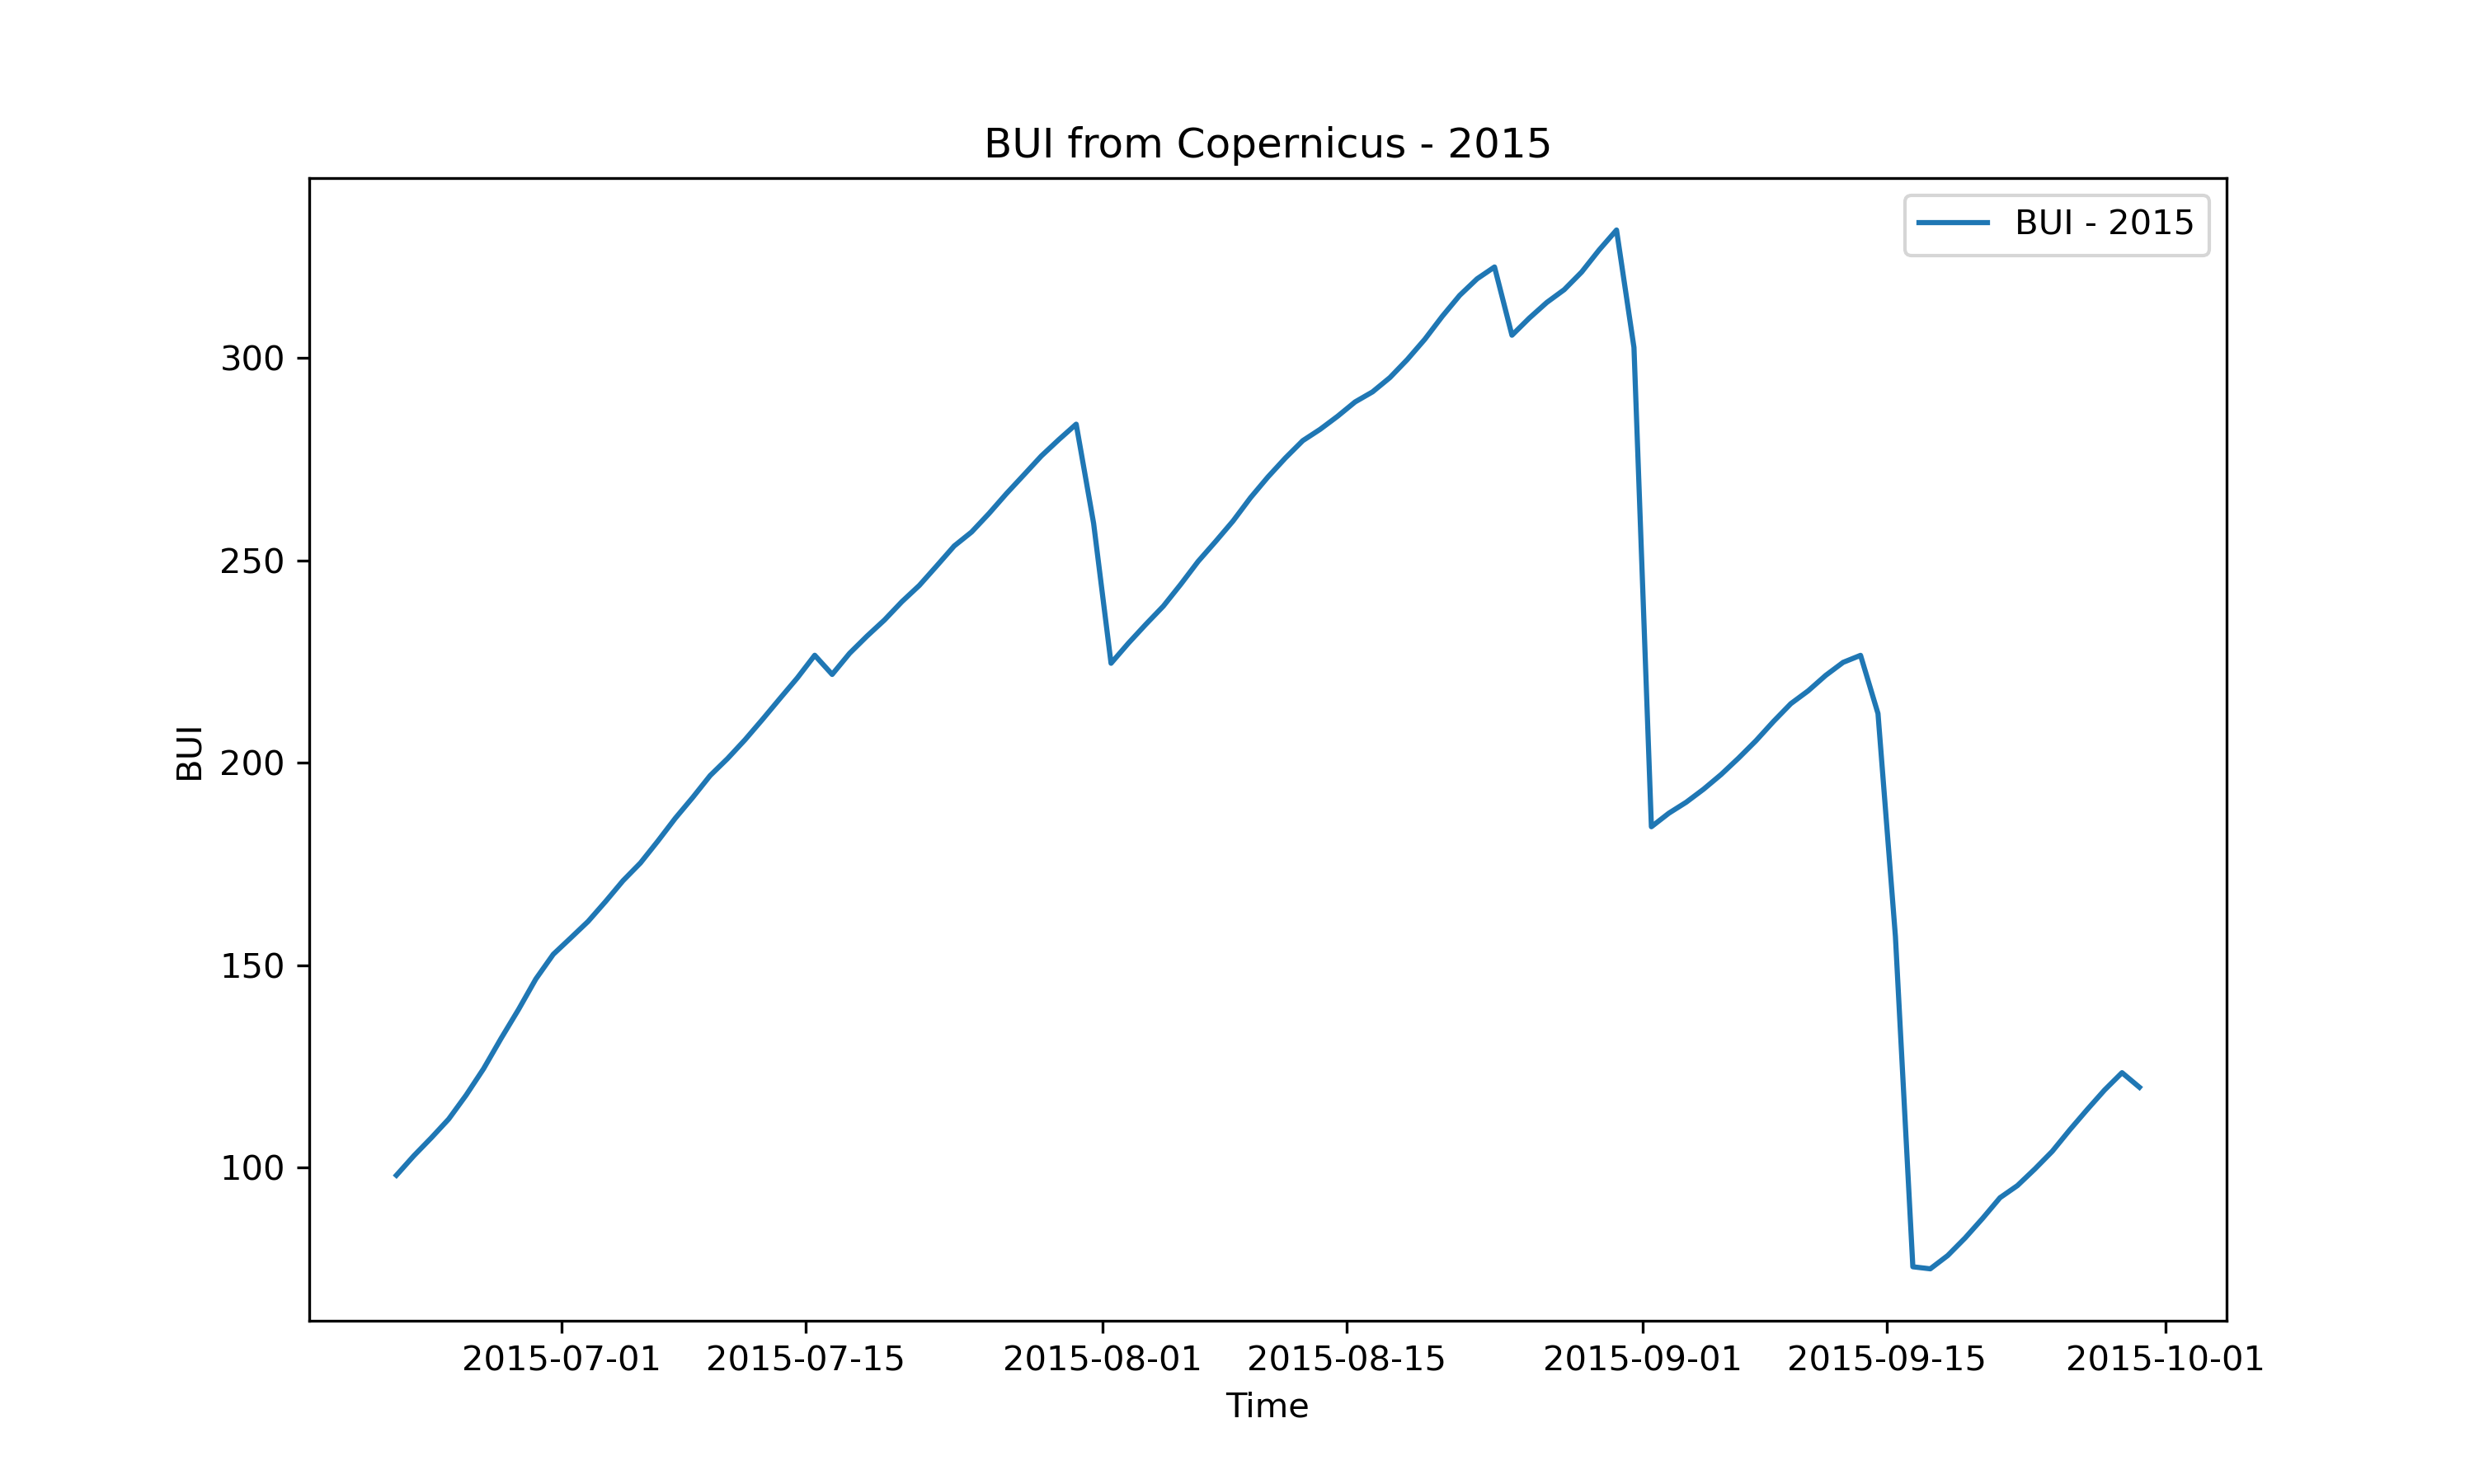
\includegraphics[width=\textwidth]{graphs/2015/2015CopernicusBUI12.png}
		\caption{Caption for image 1}
		\label{fig:img1}
	\end{subfigure}
	\hfill
	\begin{subfigure}{0.49\textwidth}
		\centering
		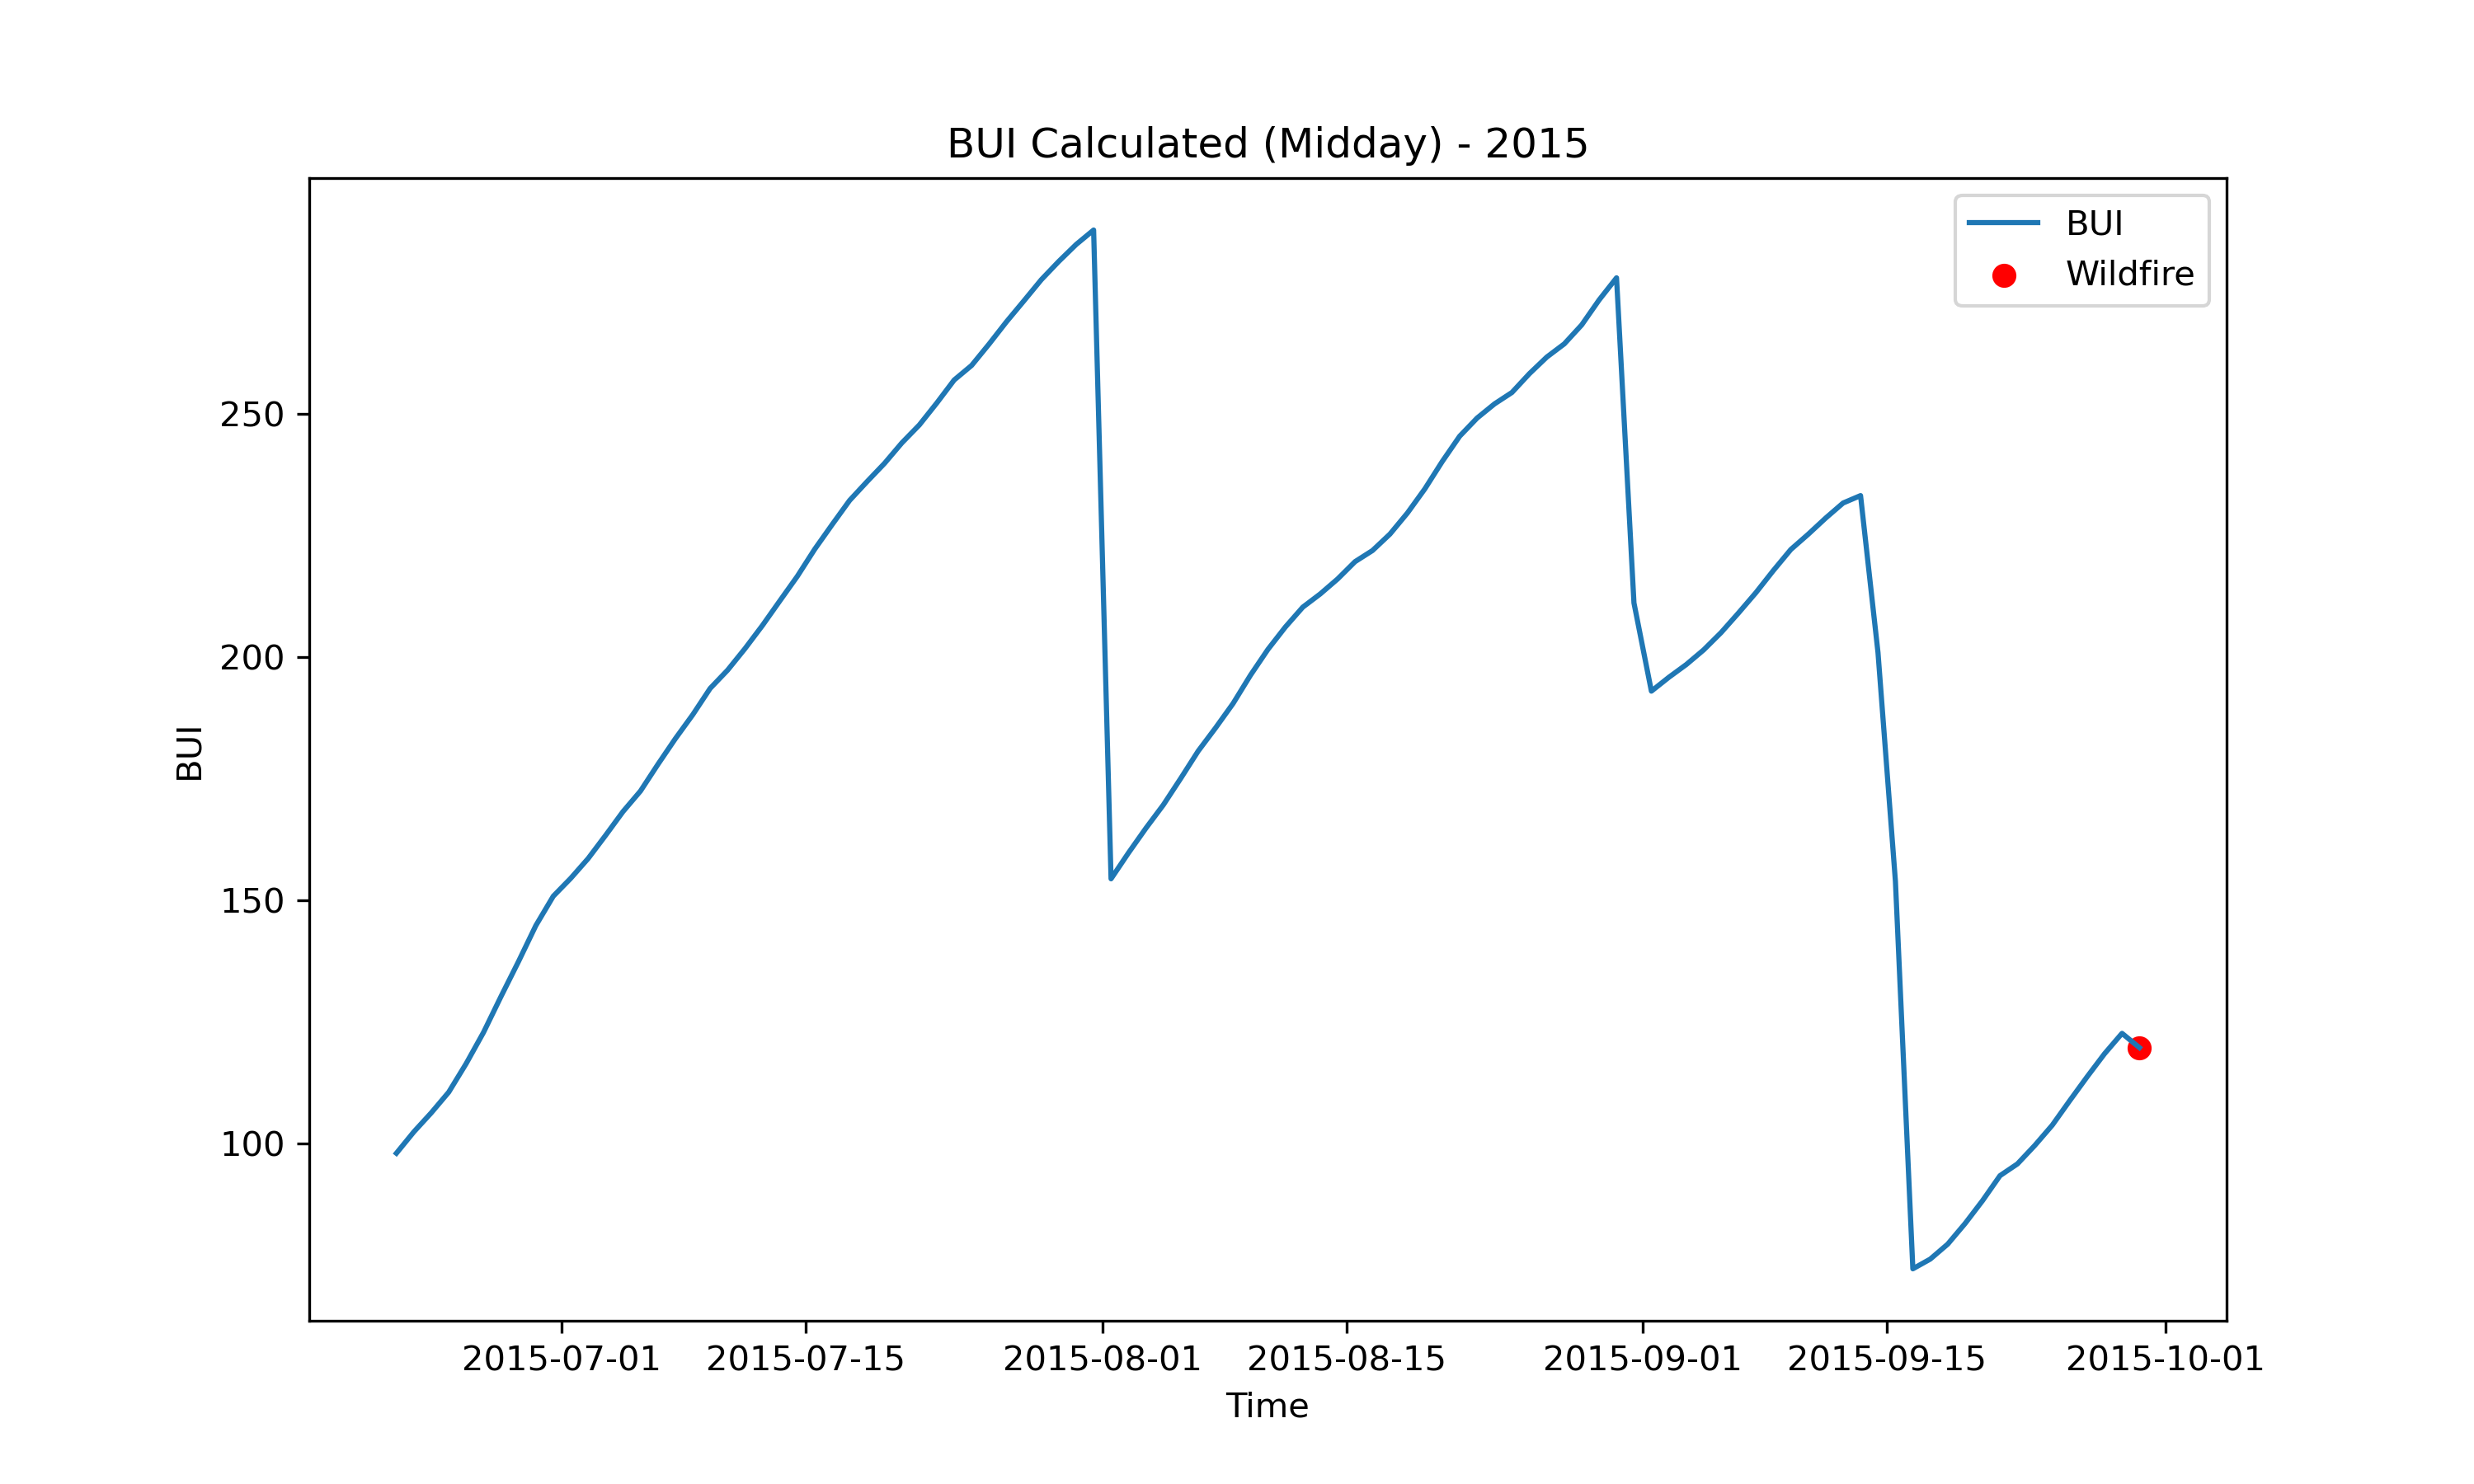
\includegraphics[width=\textwidth]{graphs/2015/2015CalcBUI12.png}
		\caption{Caption for image 2}
		\label{fig:img2}
	\end{subfigure}
	\label{fig:both_images}
\end{figure}

\begin{figure}[h]
	\caption{HELLo}
	\centering
	\begin{subfigure}{0.49\textwidth}
		\centering
		\includegraphics[width=\textwidth]{graphs/2022/2022CalcFWIX.png}
		\caption{Caption for image 1}
		\label{fig:img1}
	\end{subfigure}
	\hfill
	\begin{subfigure}{0.49\textwidth}
		\centering
		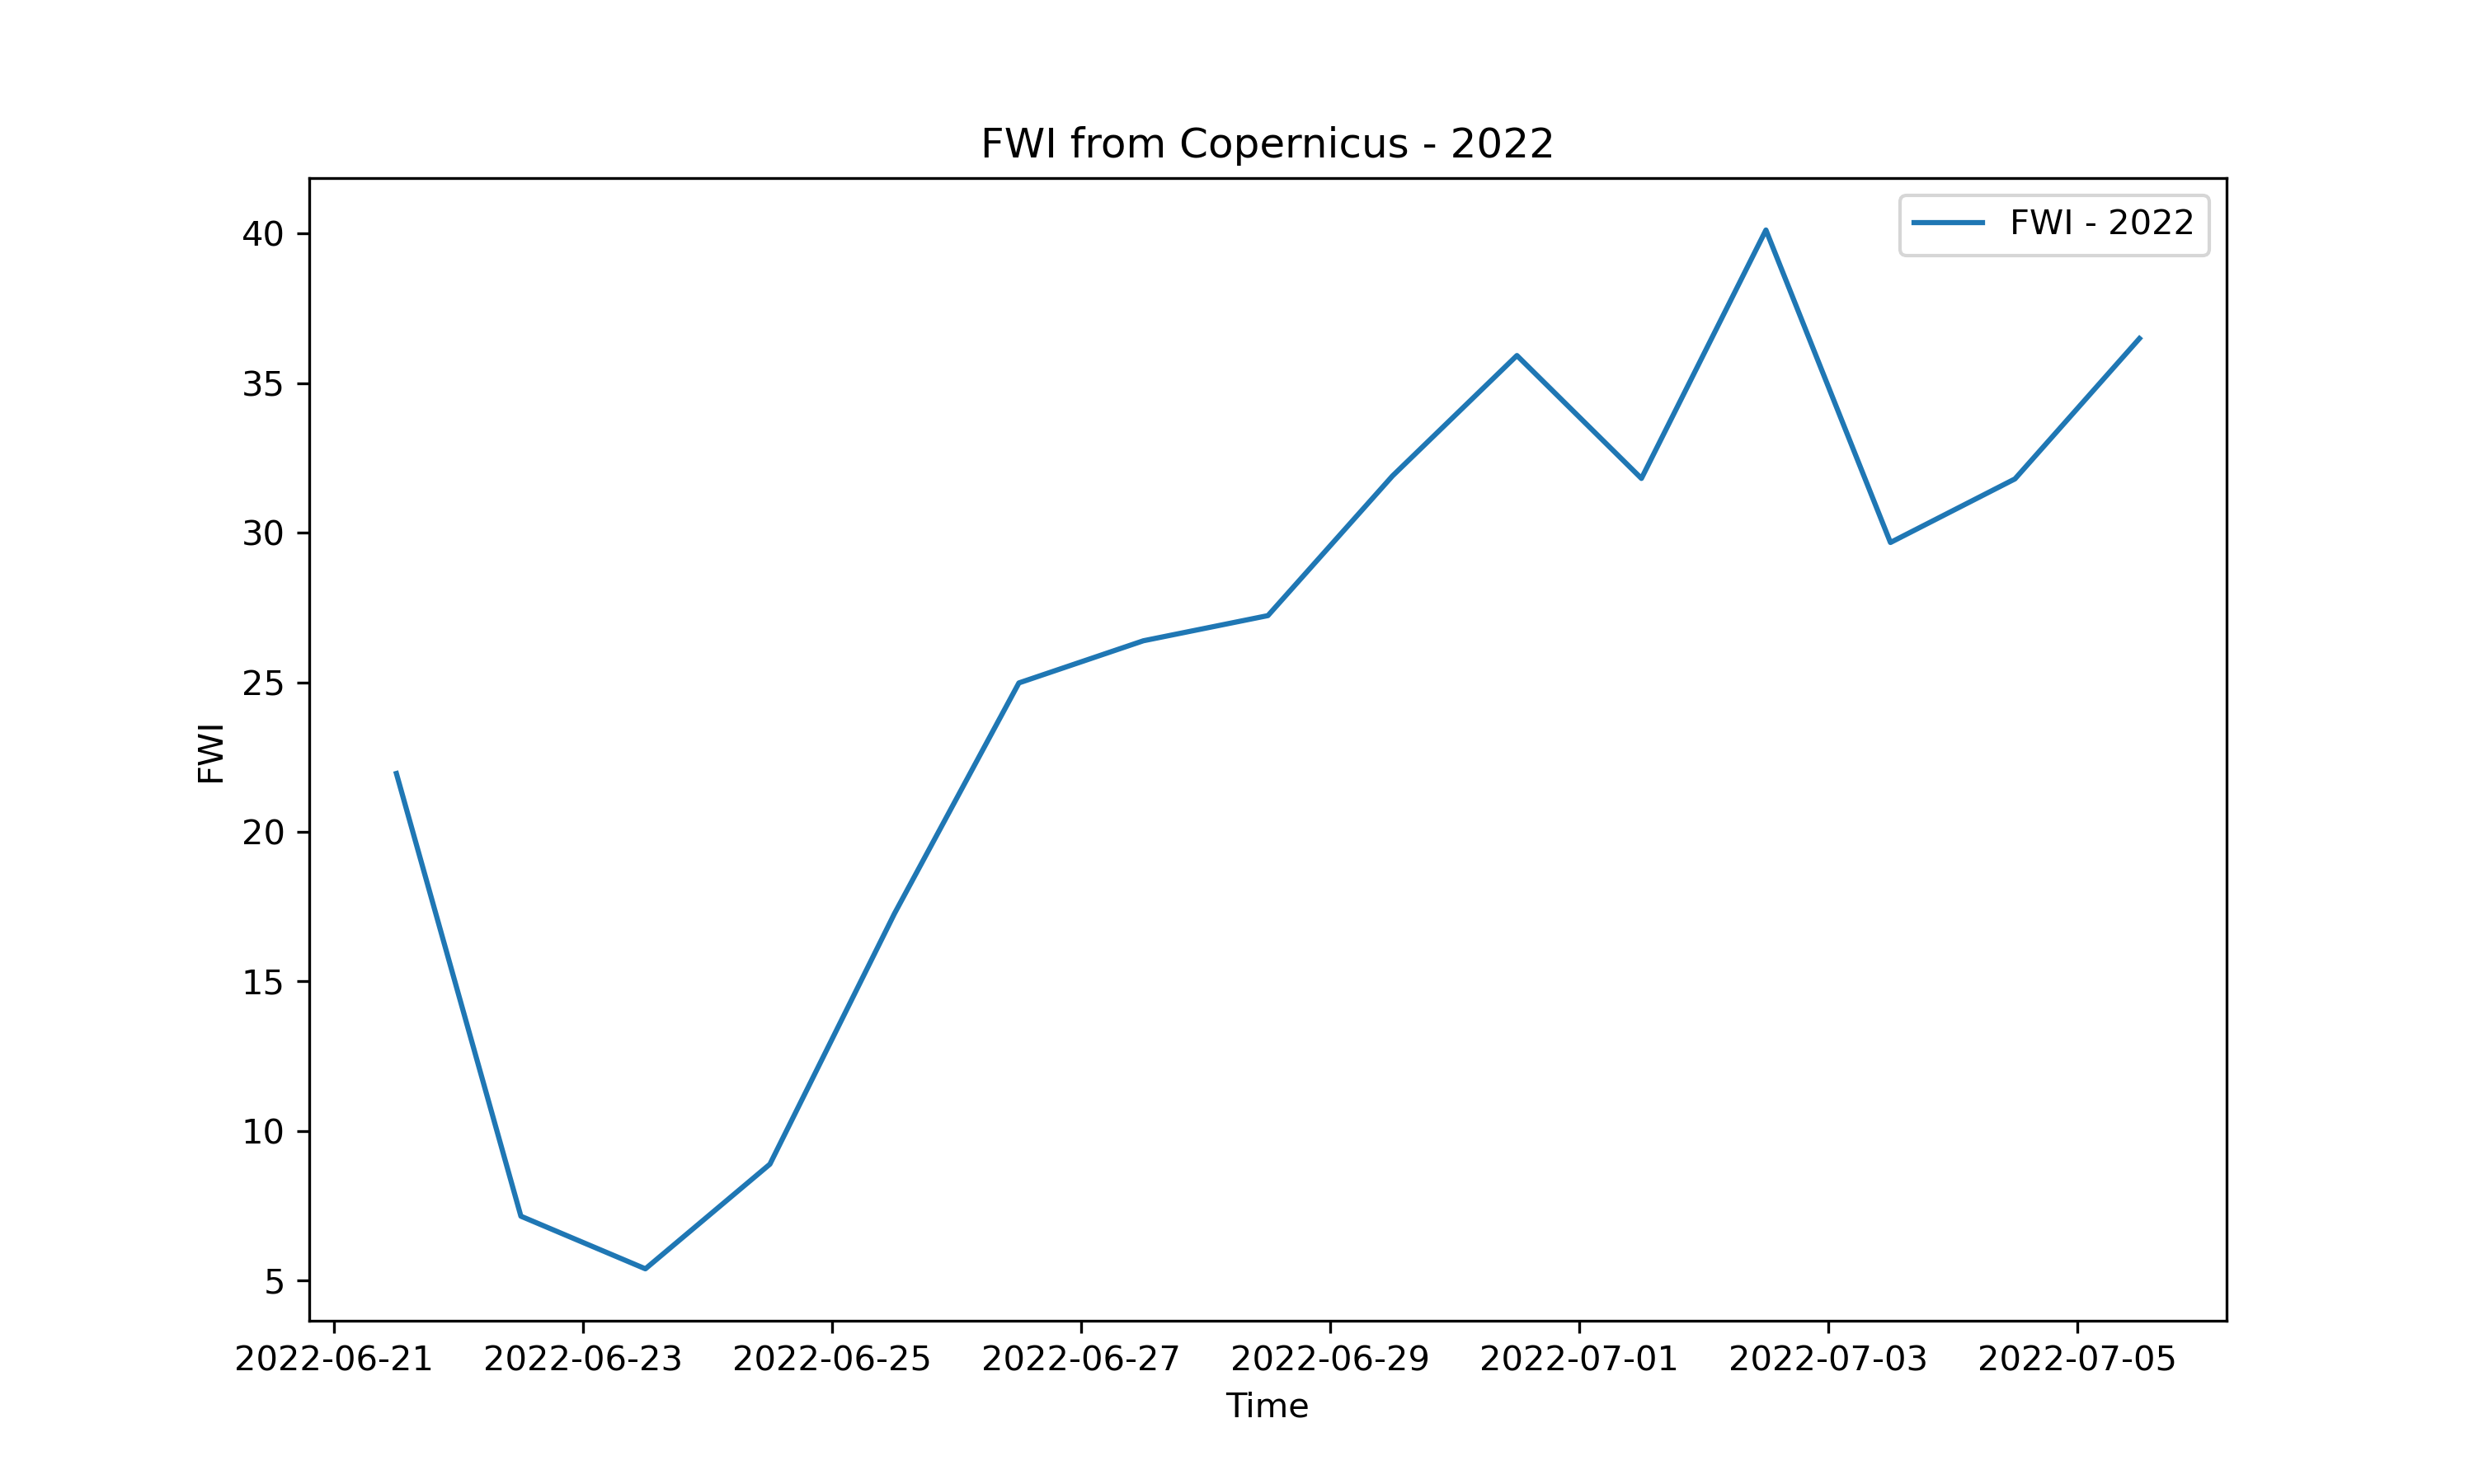
\includegraphics[width=\textwidth]{graphs/2022/2022CopernicusFWI12.png}
		\caption{Caption for image 2}
		\label{fig:img2}
	\end{subfigure}
	\label{fig:both_images}
\end{figure}

\FloatBarrier

\section{Hourly FWI variables}
\begin{figure}[h]
	\centering
	\caption{Caption for the whole figure}
	\begin{subfigure}{0.3\textwidth}
		\centering
		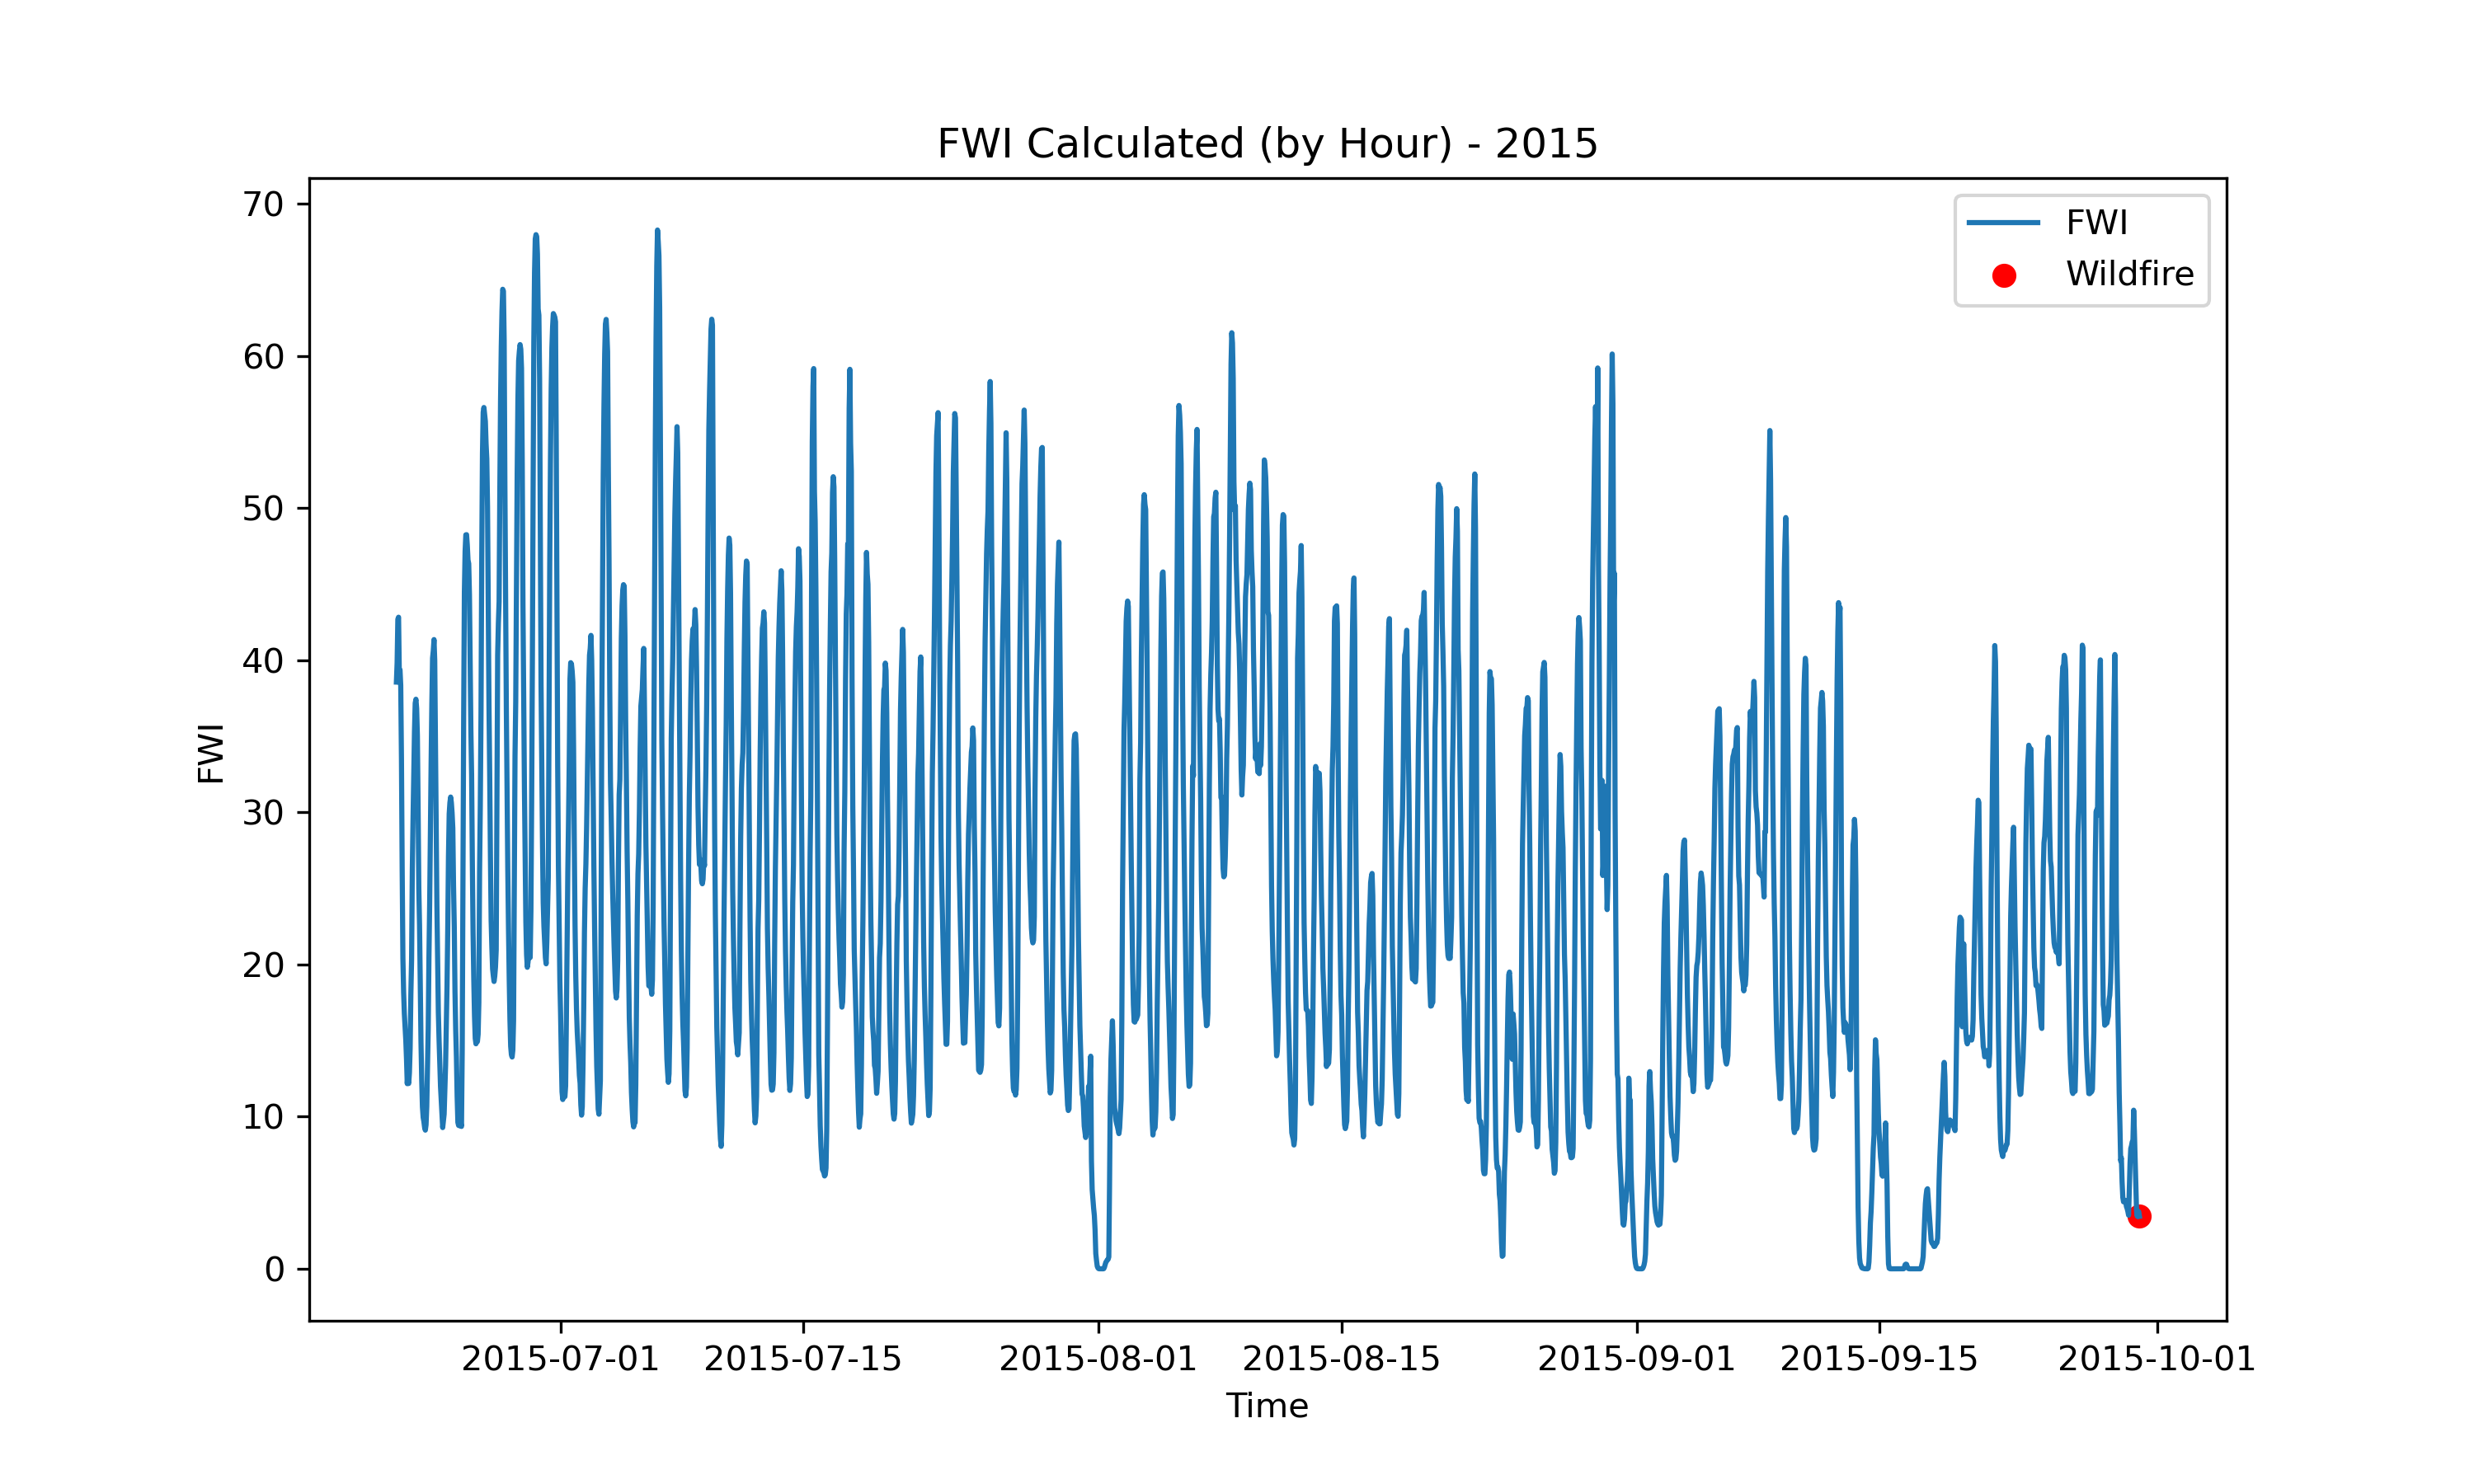
\includegraphics[width=\textwidth]{graphs/2015/byHour/2015CalcFWI12.png}
		\caption{Caption for image 1}
		\label{fig:img1}
	\end{subfigure}
	\hfill
	\begin{subfigure}{0.3\textwidth}
		\centering
		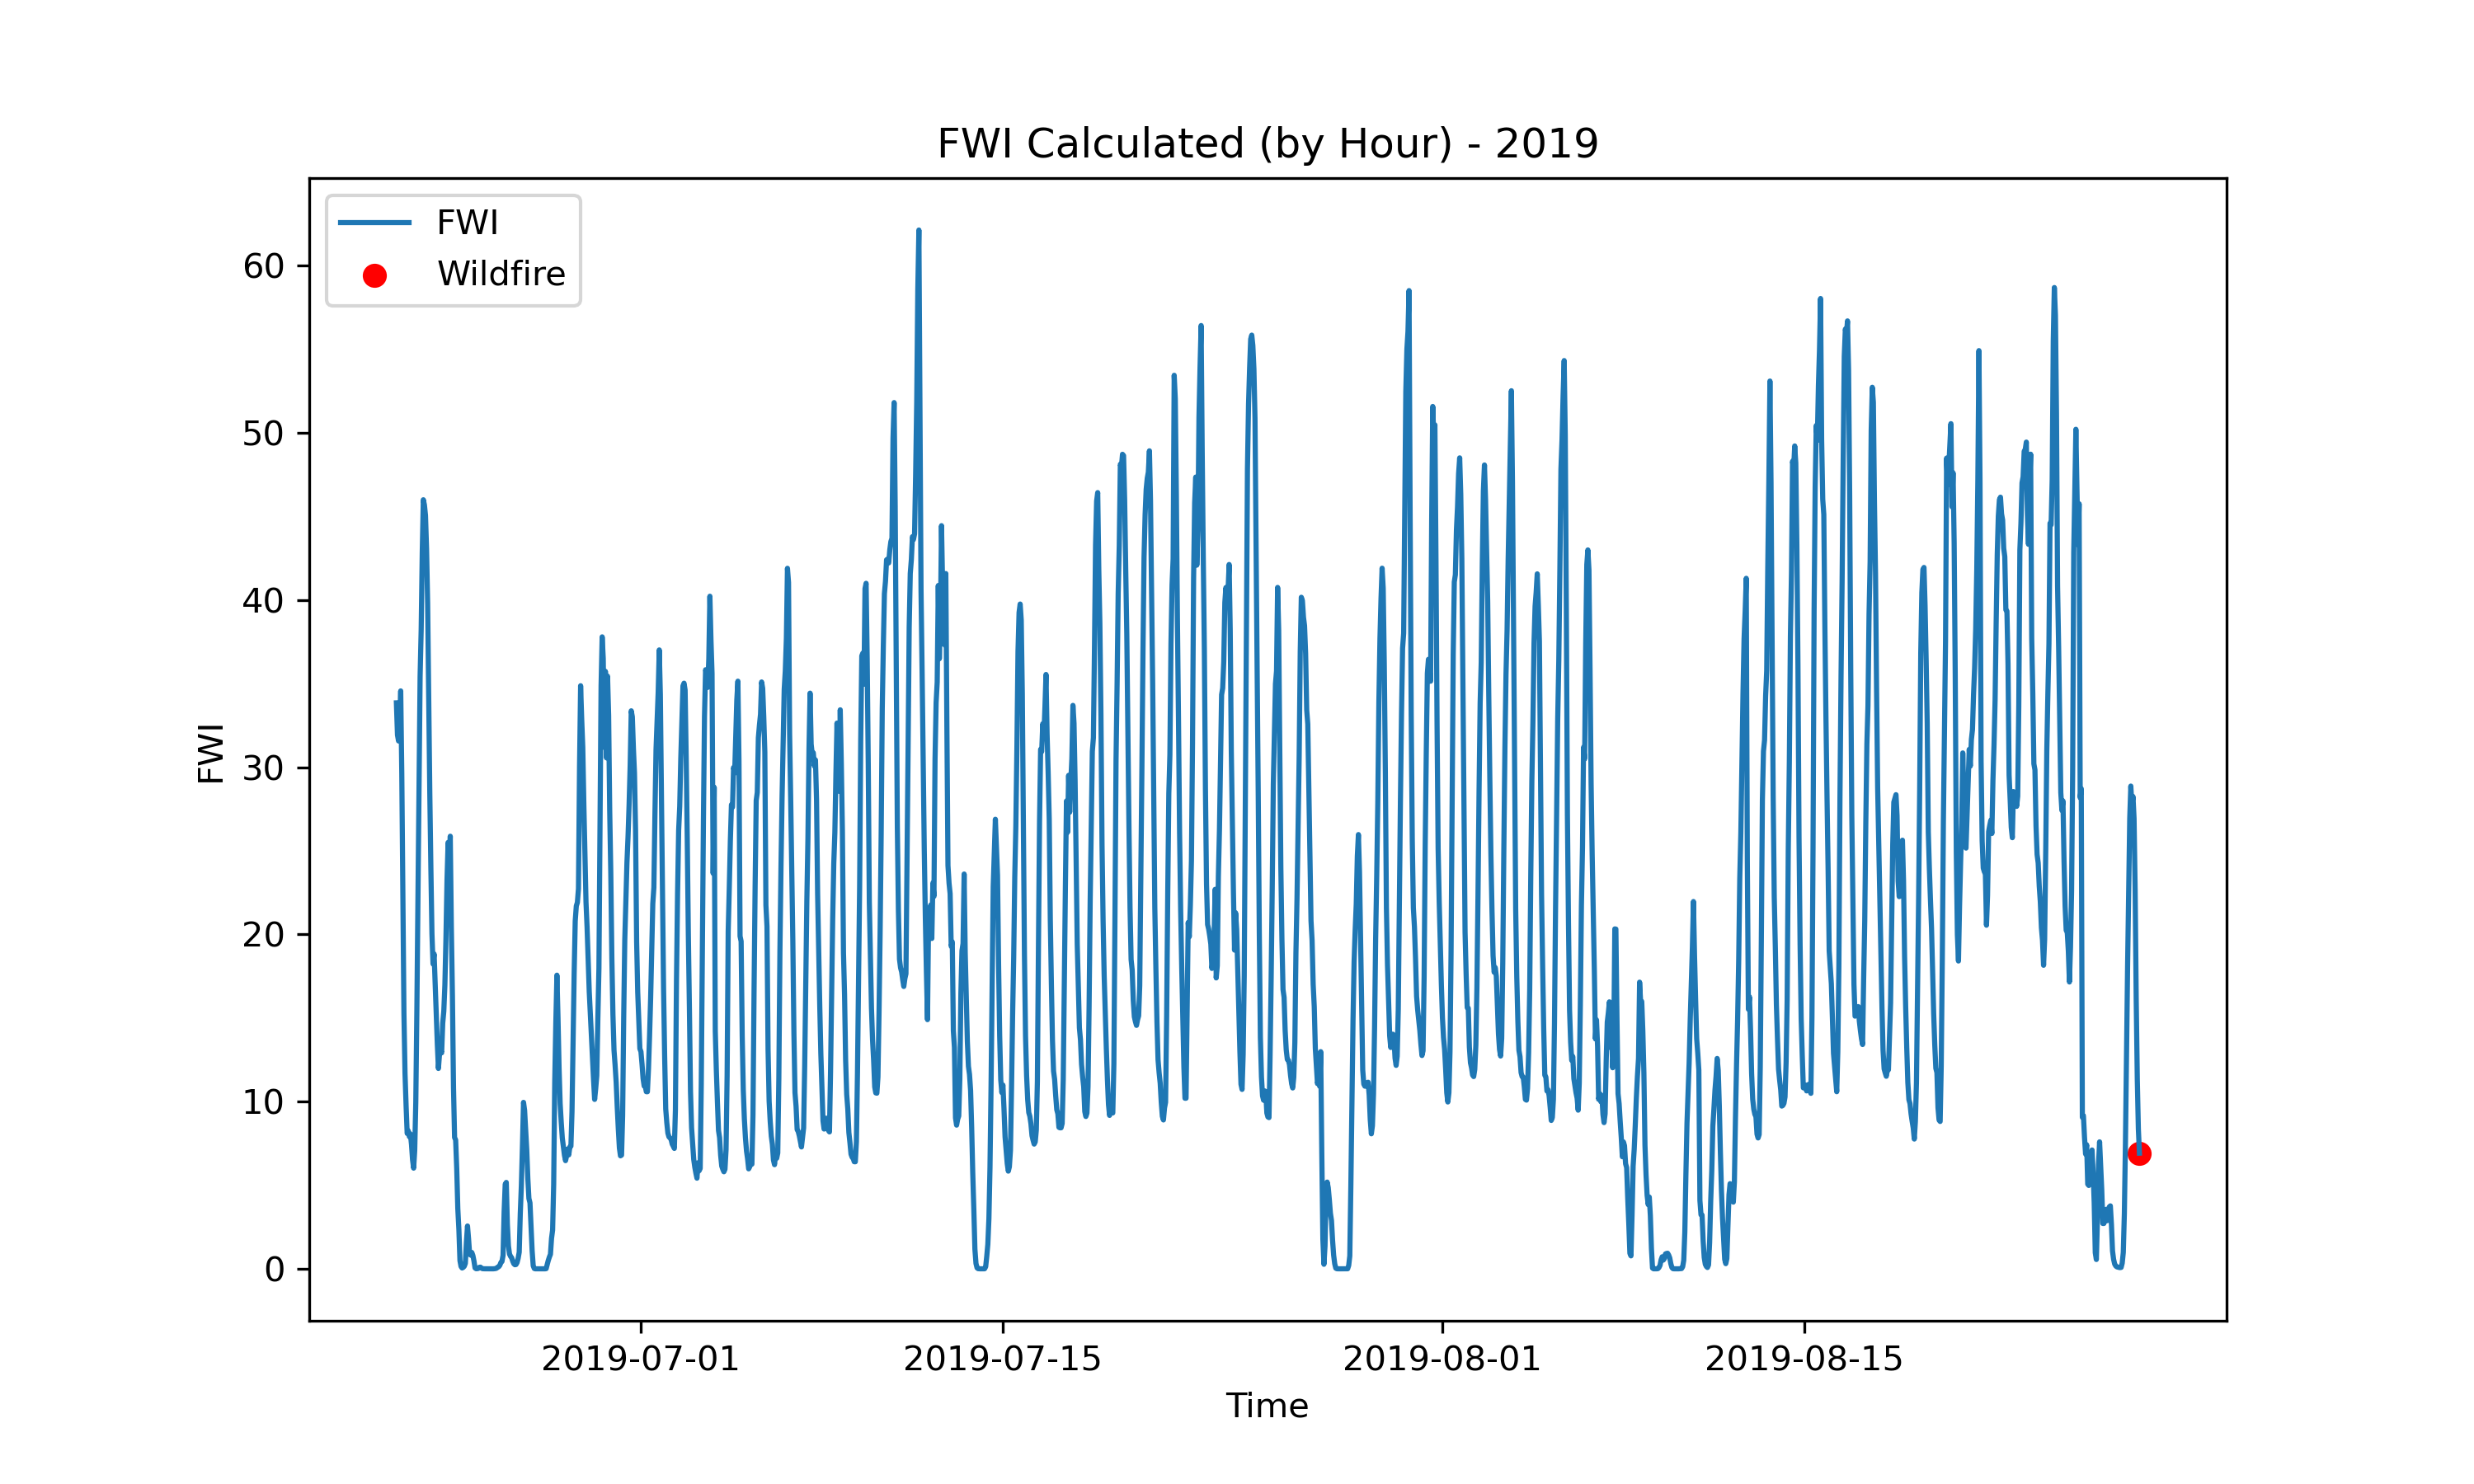
\includegraphics[width=\textwidth]{graphs/2019/byHour/2019CalcFWI12.png}
		\caption{Caption for image 2}
		\label{fig:img2}
	\end{subfigure}
	\hfill
	\begin{subfigure}{0.3\textwidth}
		\centering
		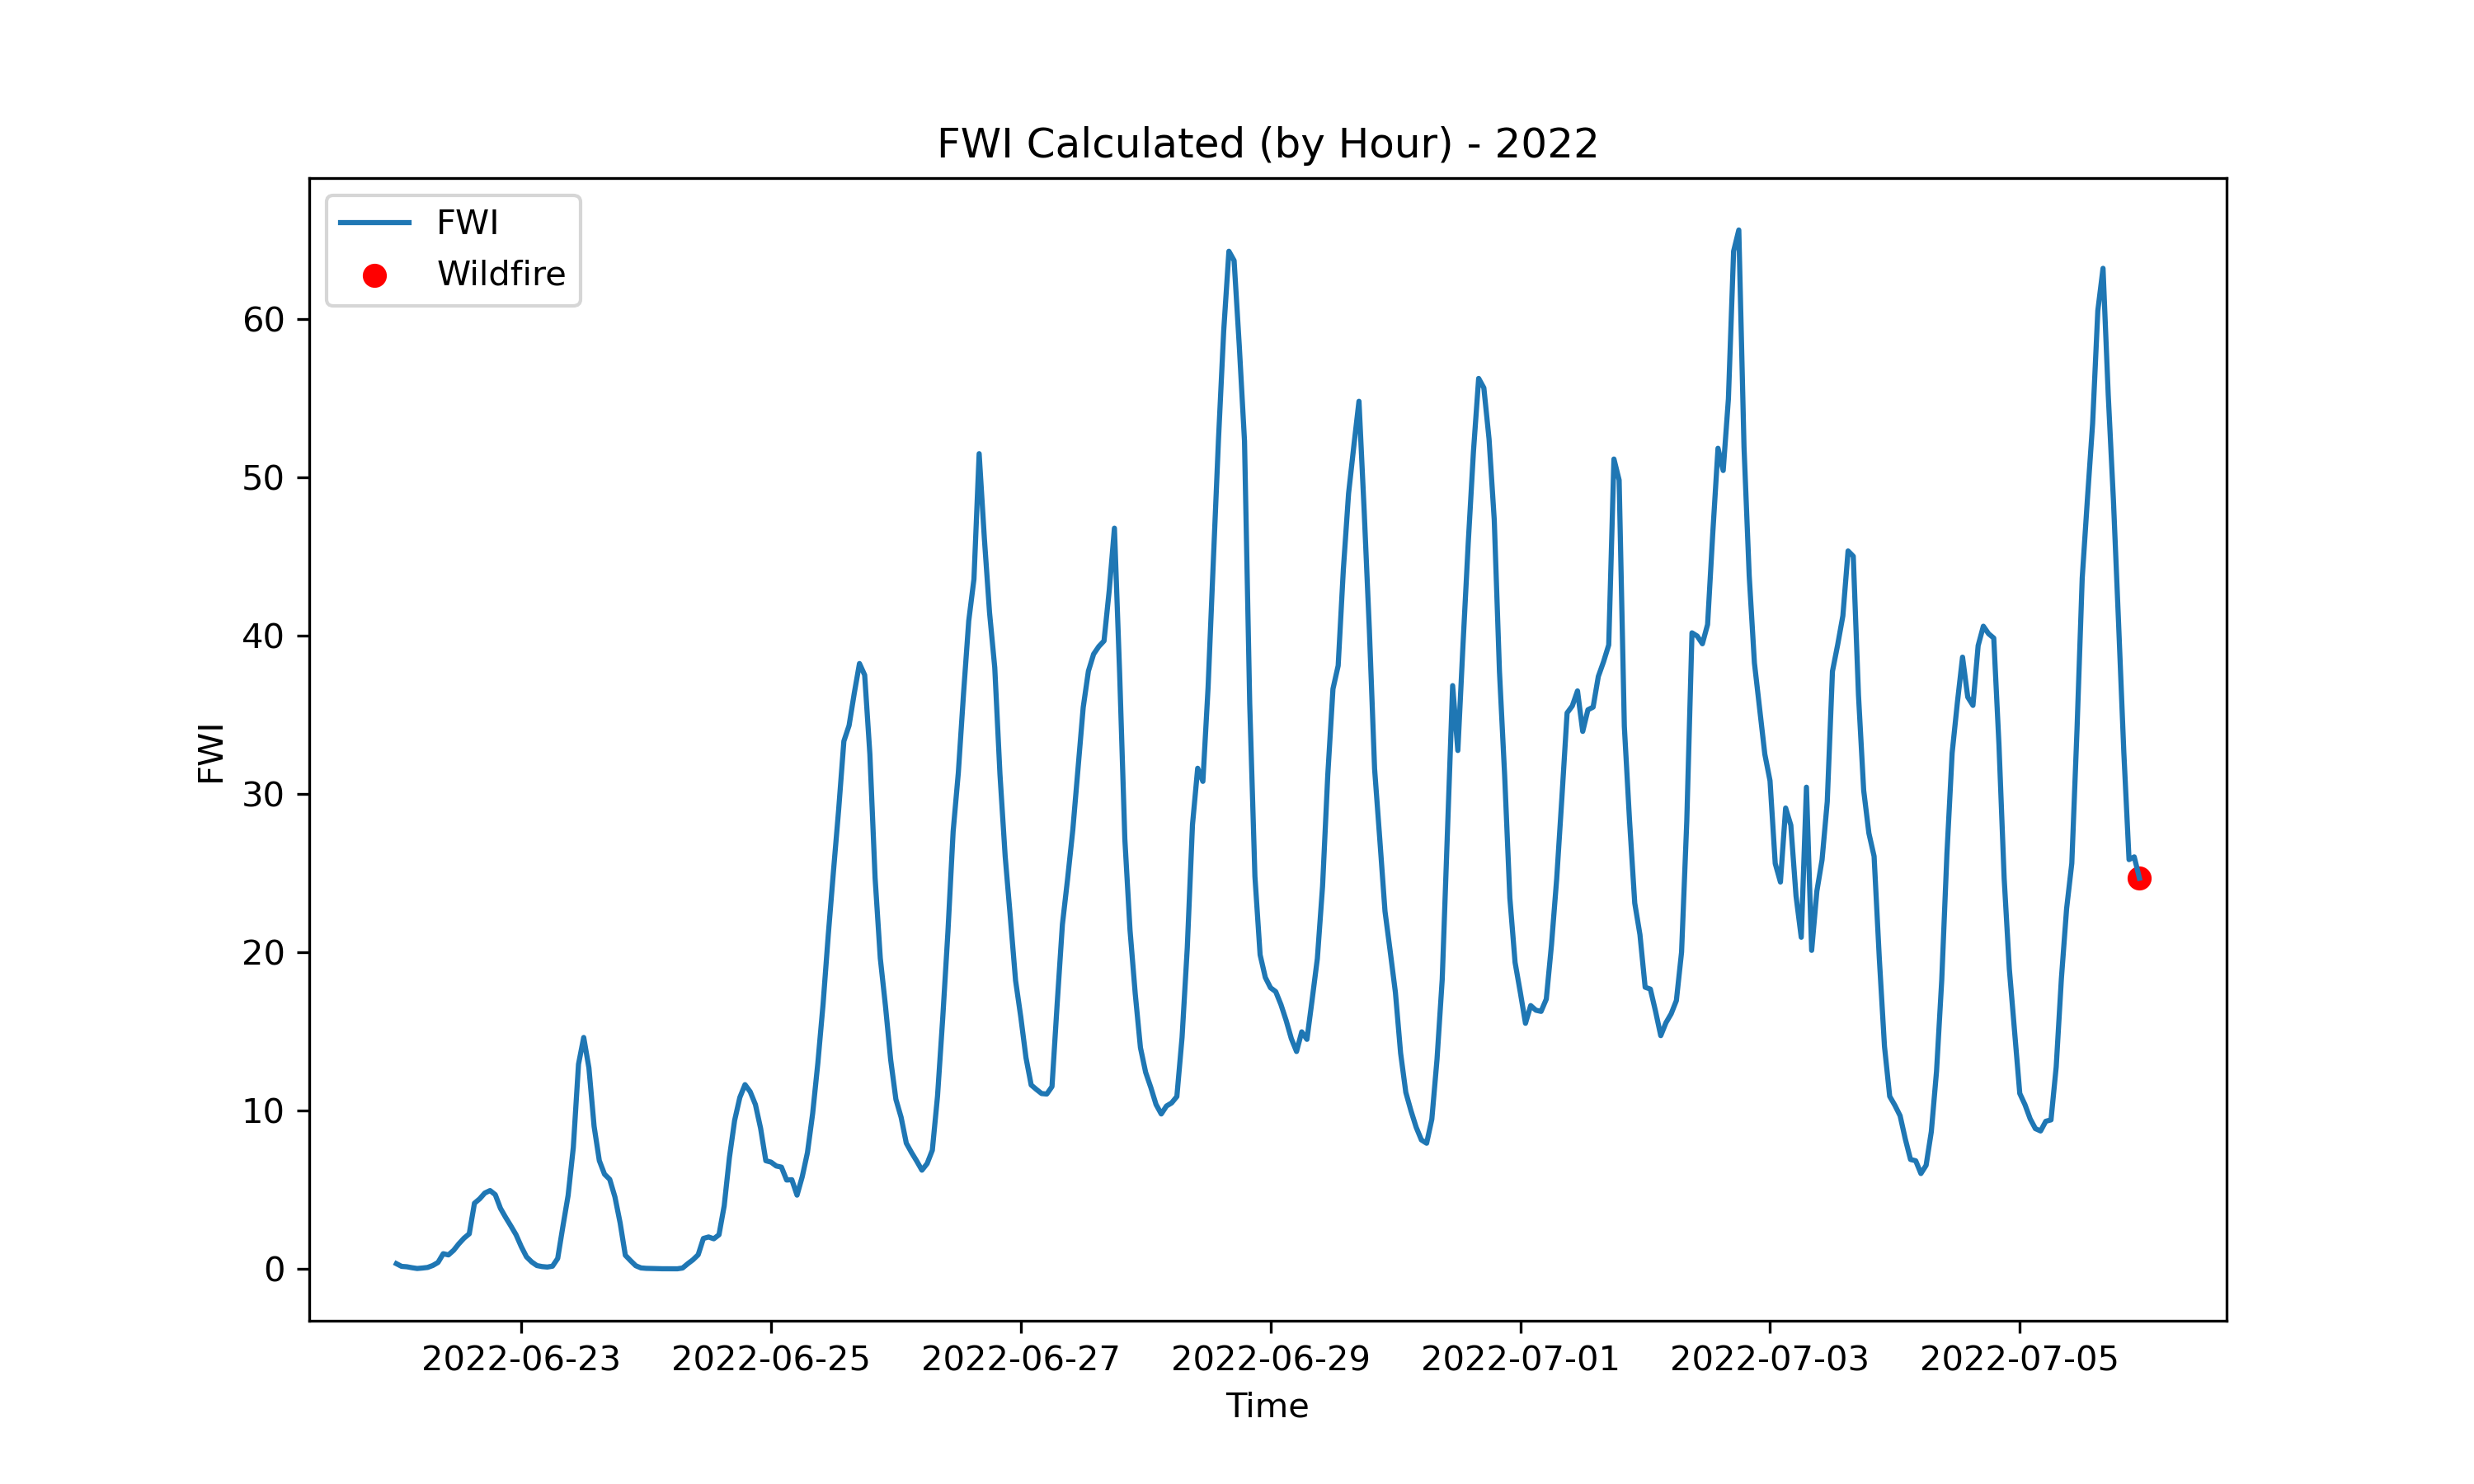
\includegraphics[width=\textwidth]{graphs/2022/2022CalcFWI12.png}
		\caption{Caption for image 3}
		\label{fig:img3}
	\end{subfigure}
	
	\label{fig:all_images}
\end{figure}

\begin{figure}[h]
	\centering
	\caption{Caption for the whole figure}
	\begin{subfigure}{0.3\textwidth}
		\centering
		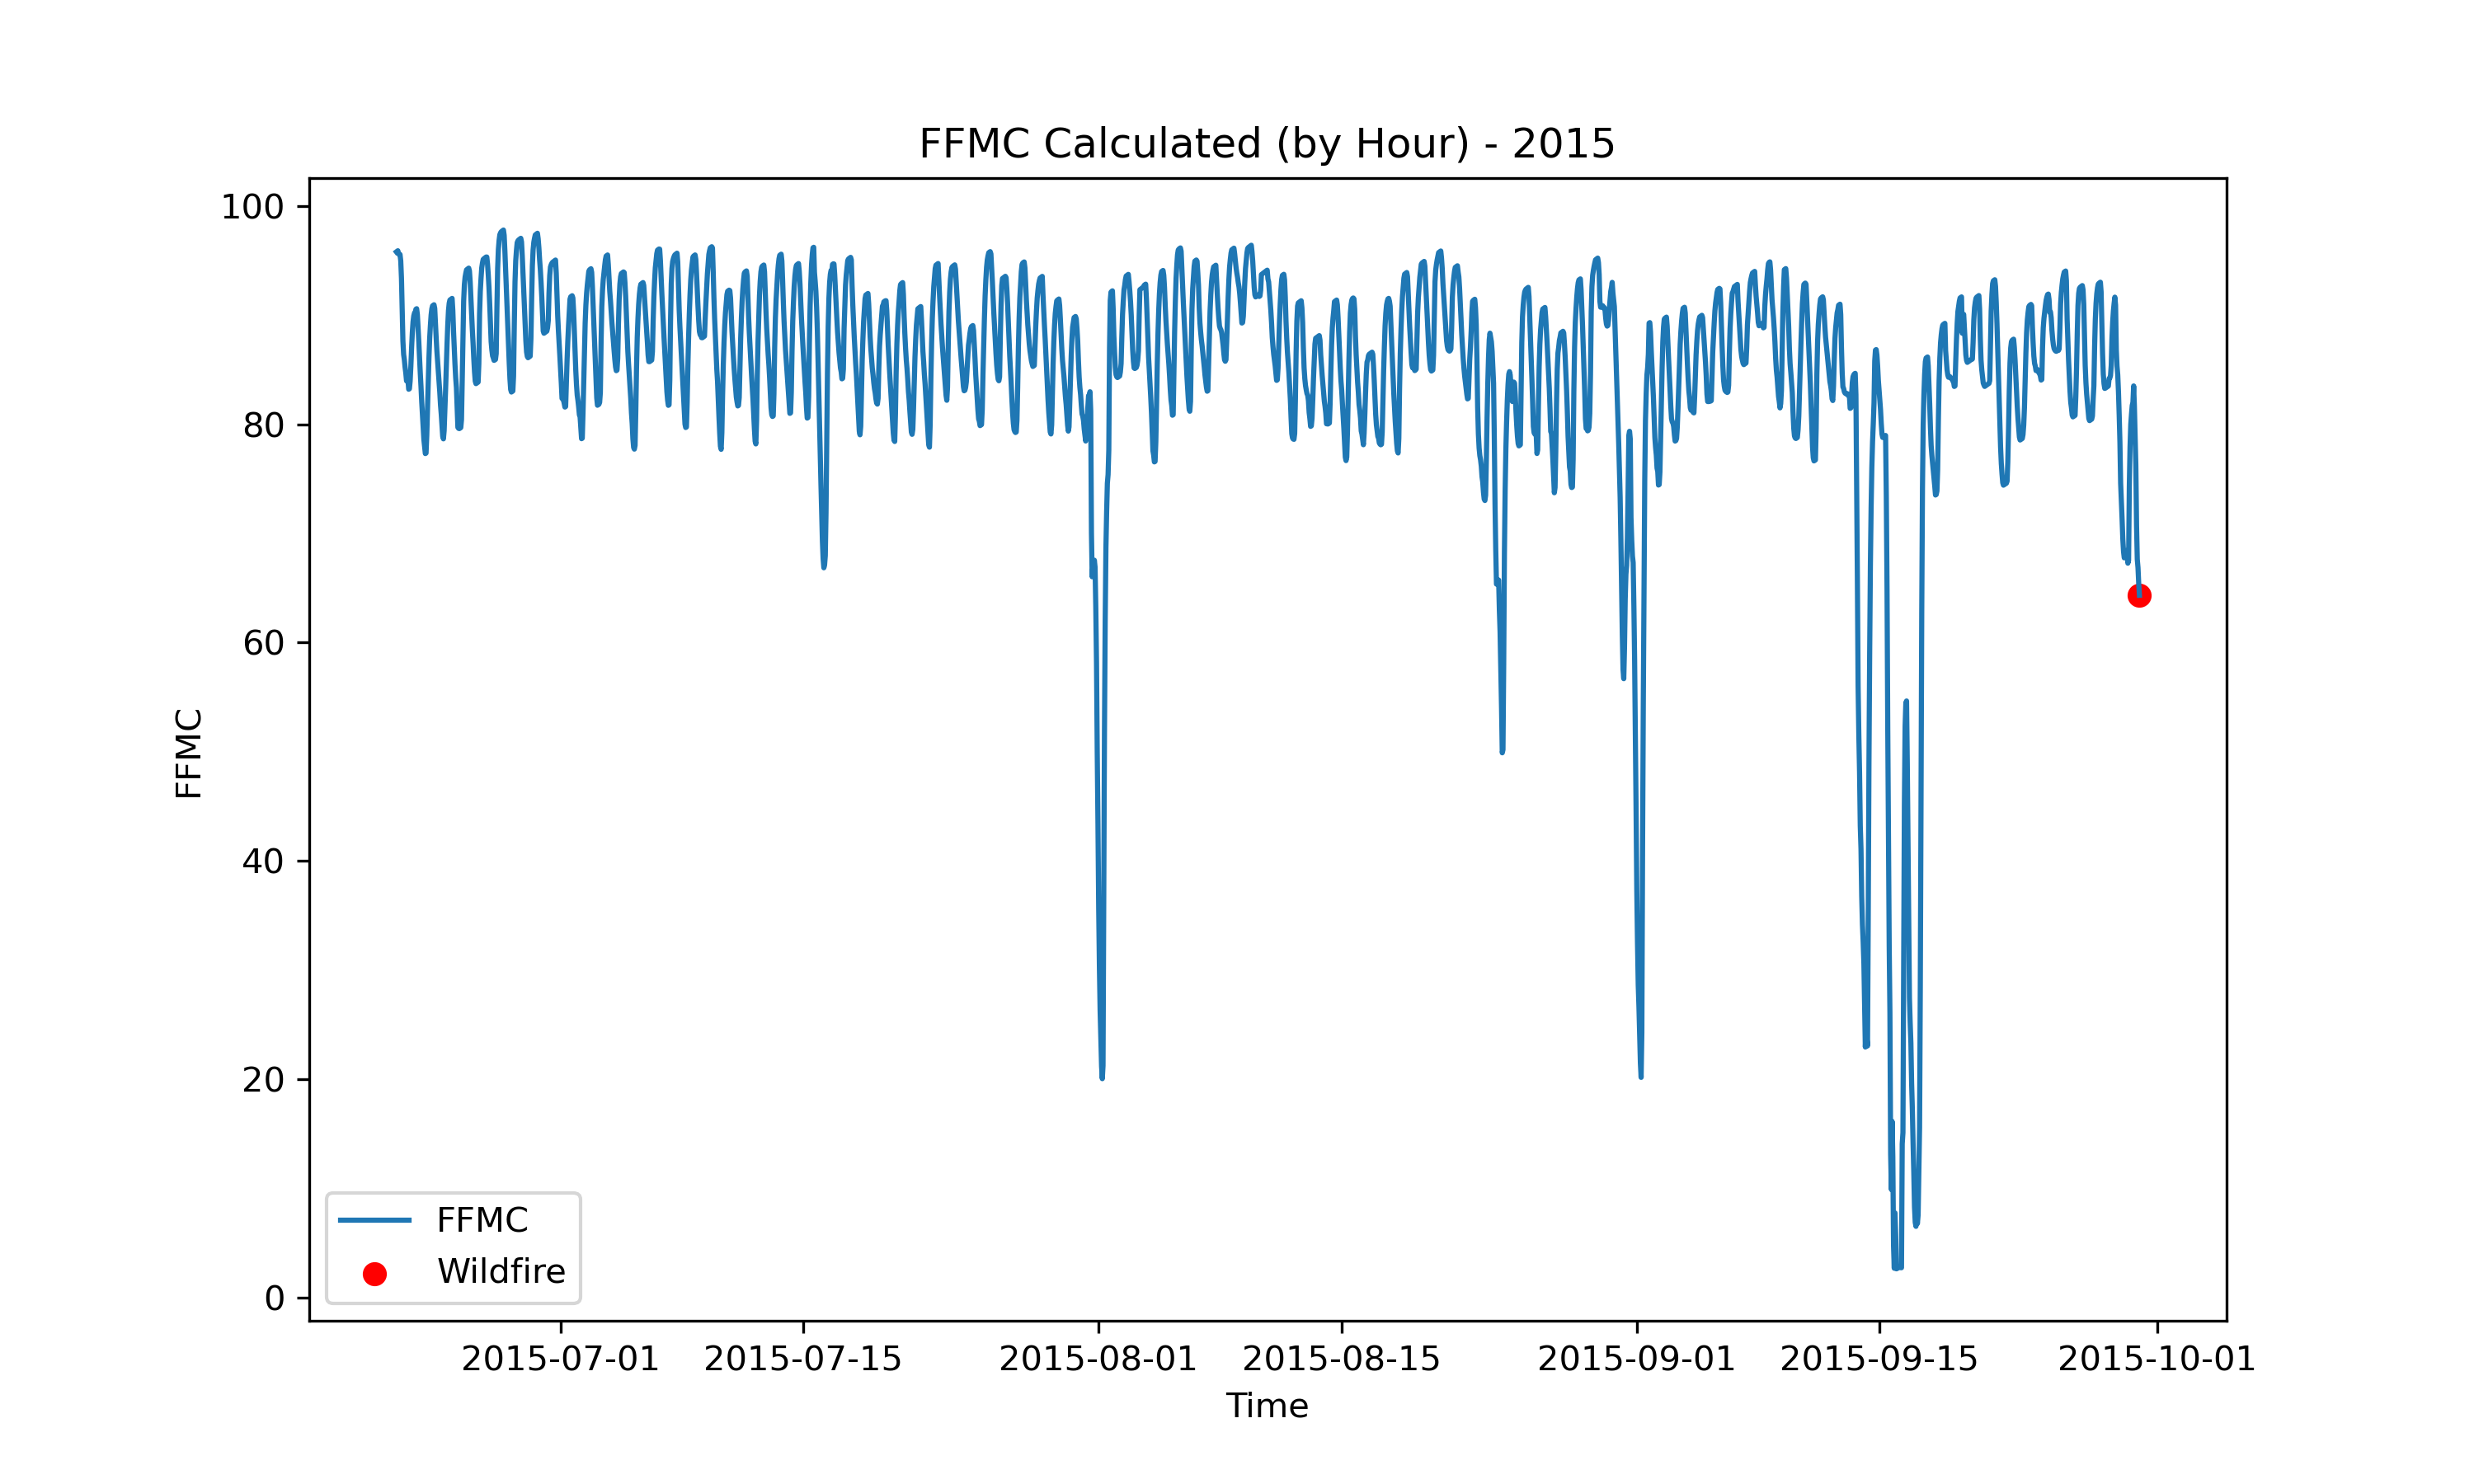
\includegraphics[width=\textwidth]{graphs/2015/byHour/2015CalcFFMC12.png}
		\caption{Caption for image 1}
		\label{fig:img1}
	\end{subfigure}
	\hfill
	\begin{subfigure}{0.3\textwidth}
		\centering
		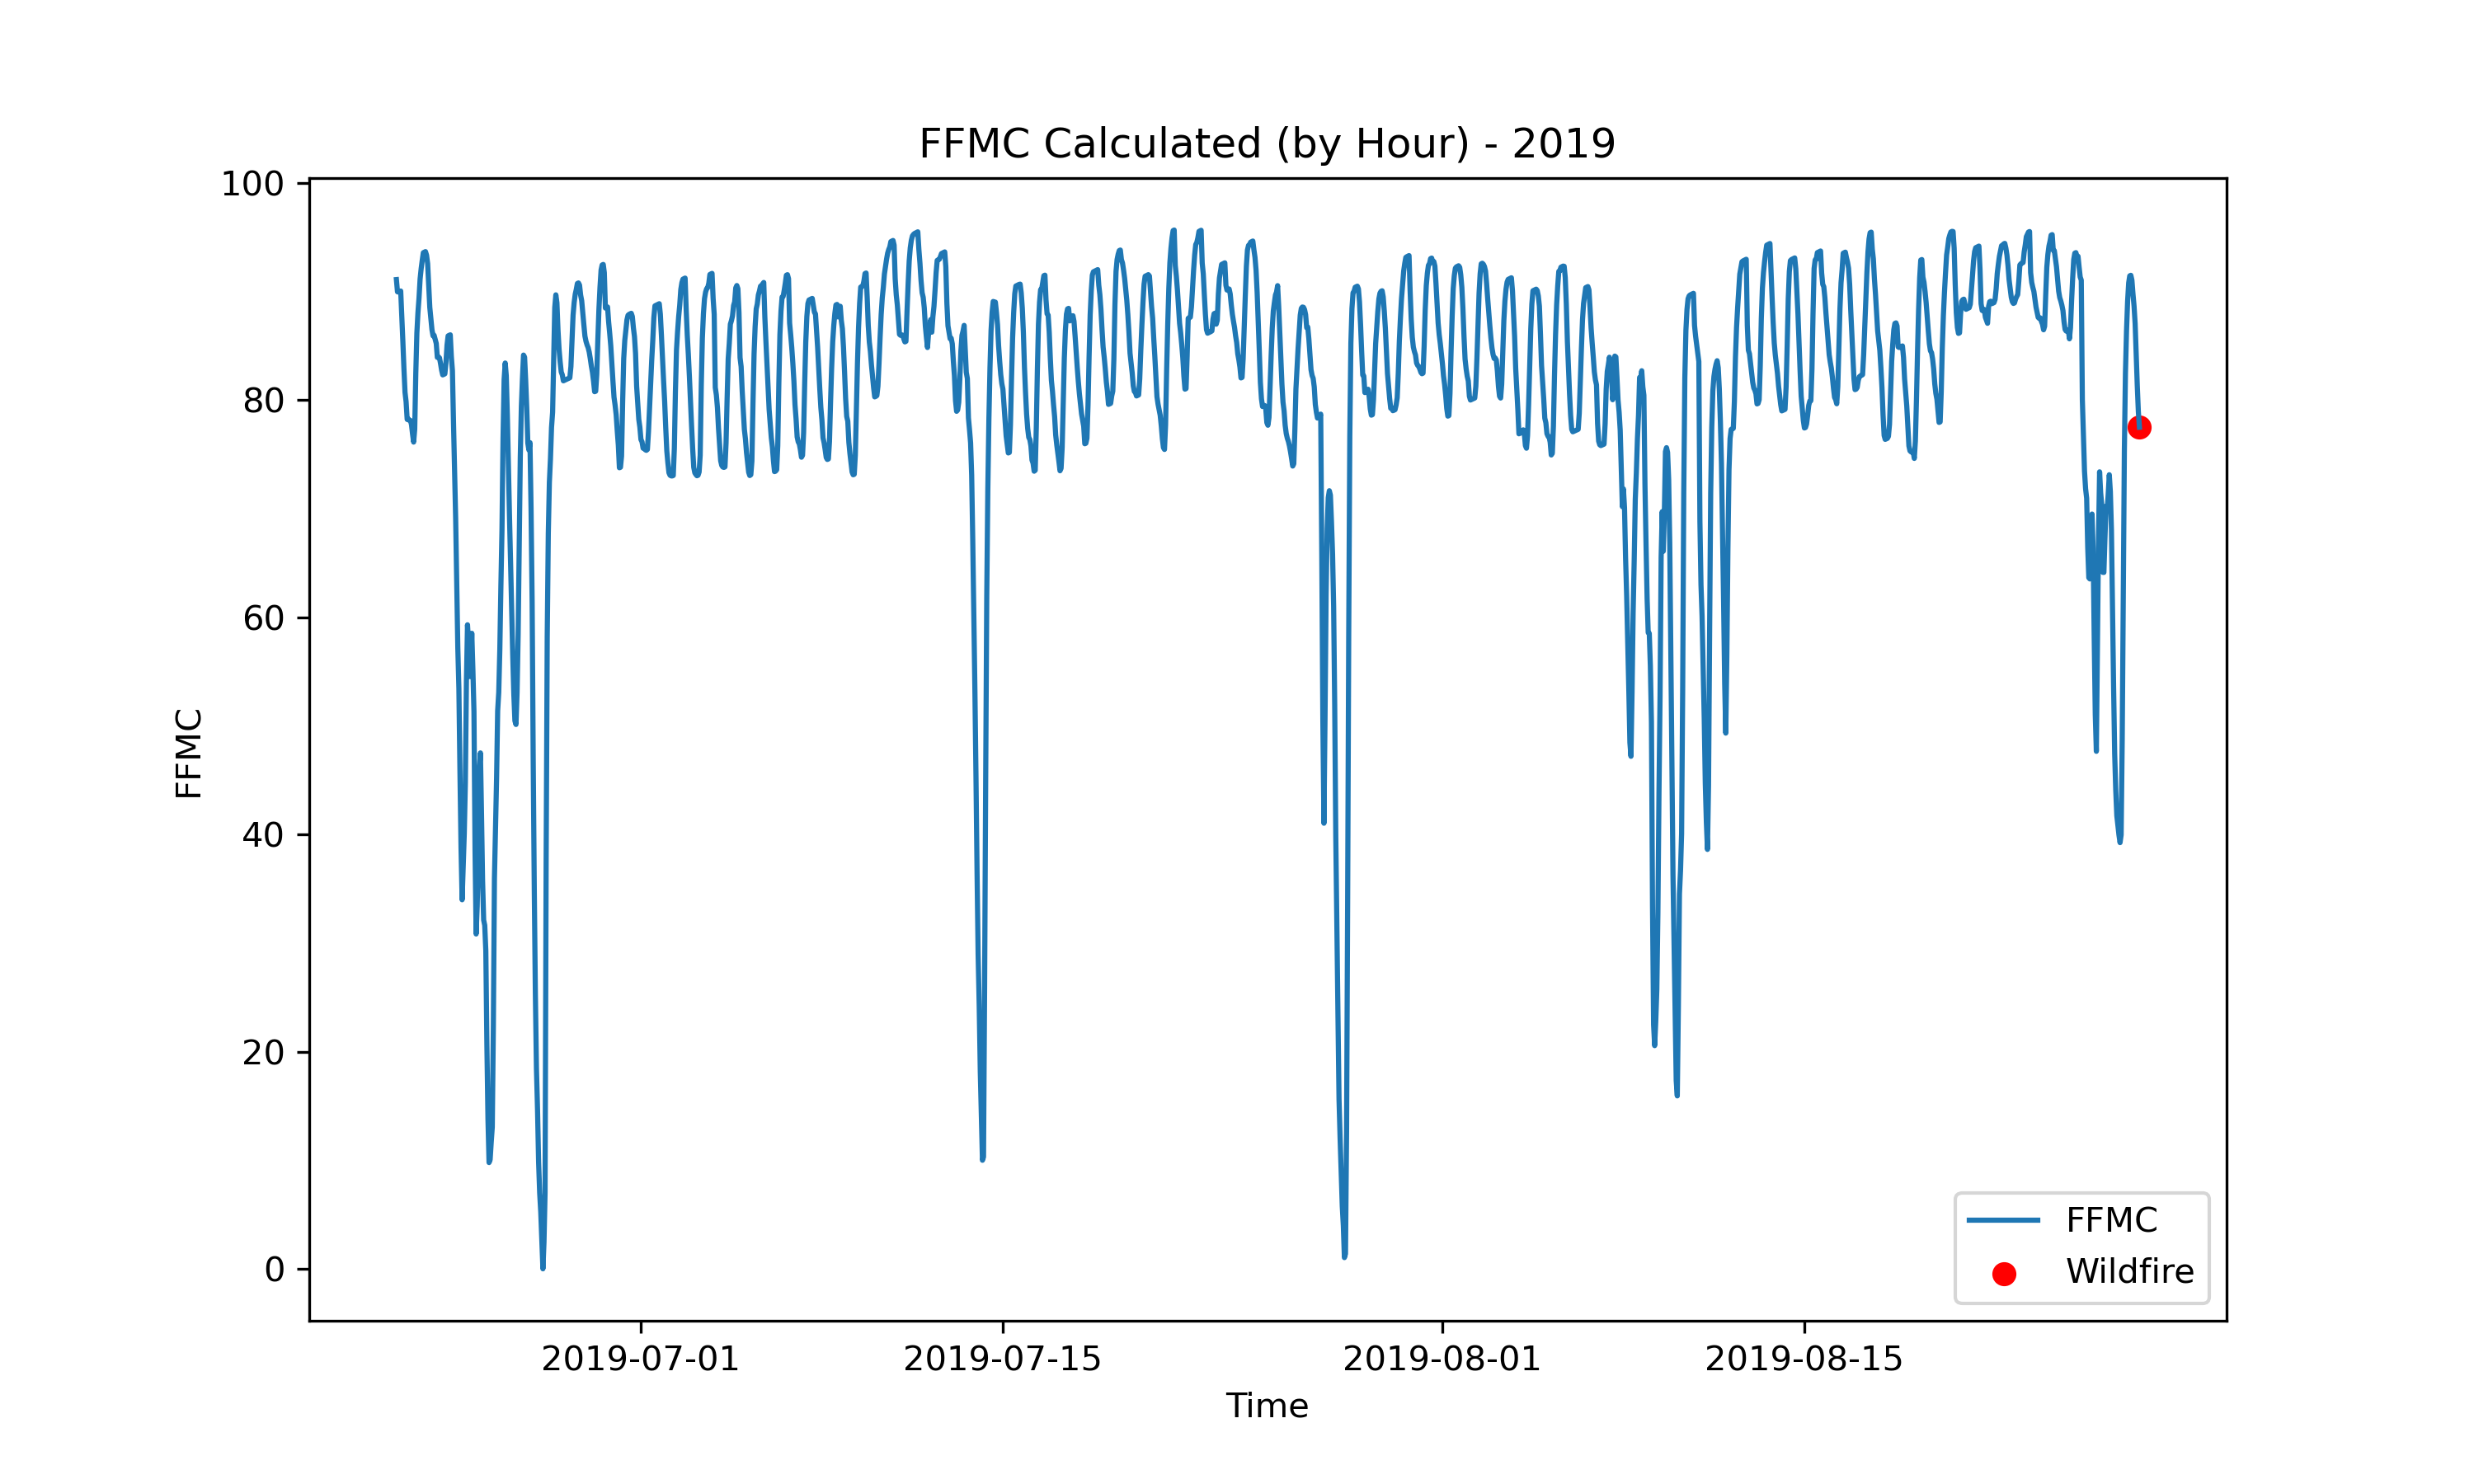
\includegraphics[width=\textwidth]{graphs/2019/byHour/2019CalcFFMC12.png}
		\caption{Caption for image 2}
		\label{fig:img2}
	\end{subfigure}
	\hfill
	\begin{subfigure}{0.3\textwidth}
		\centering
		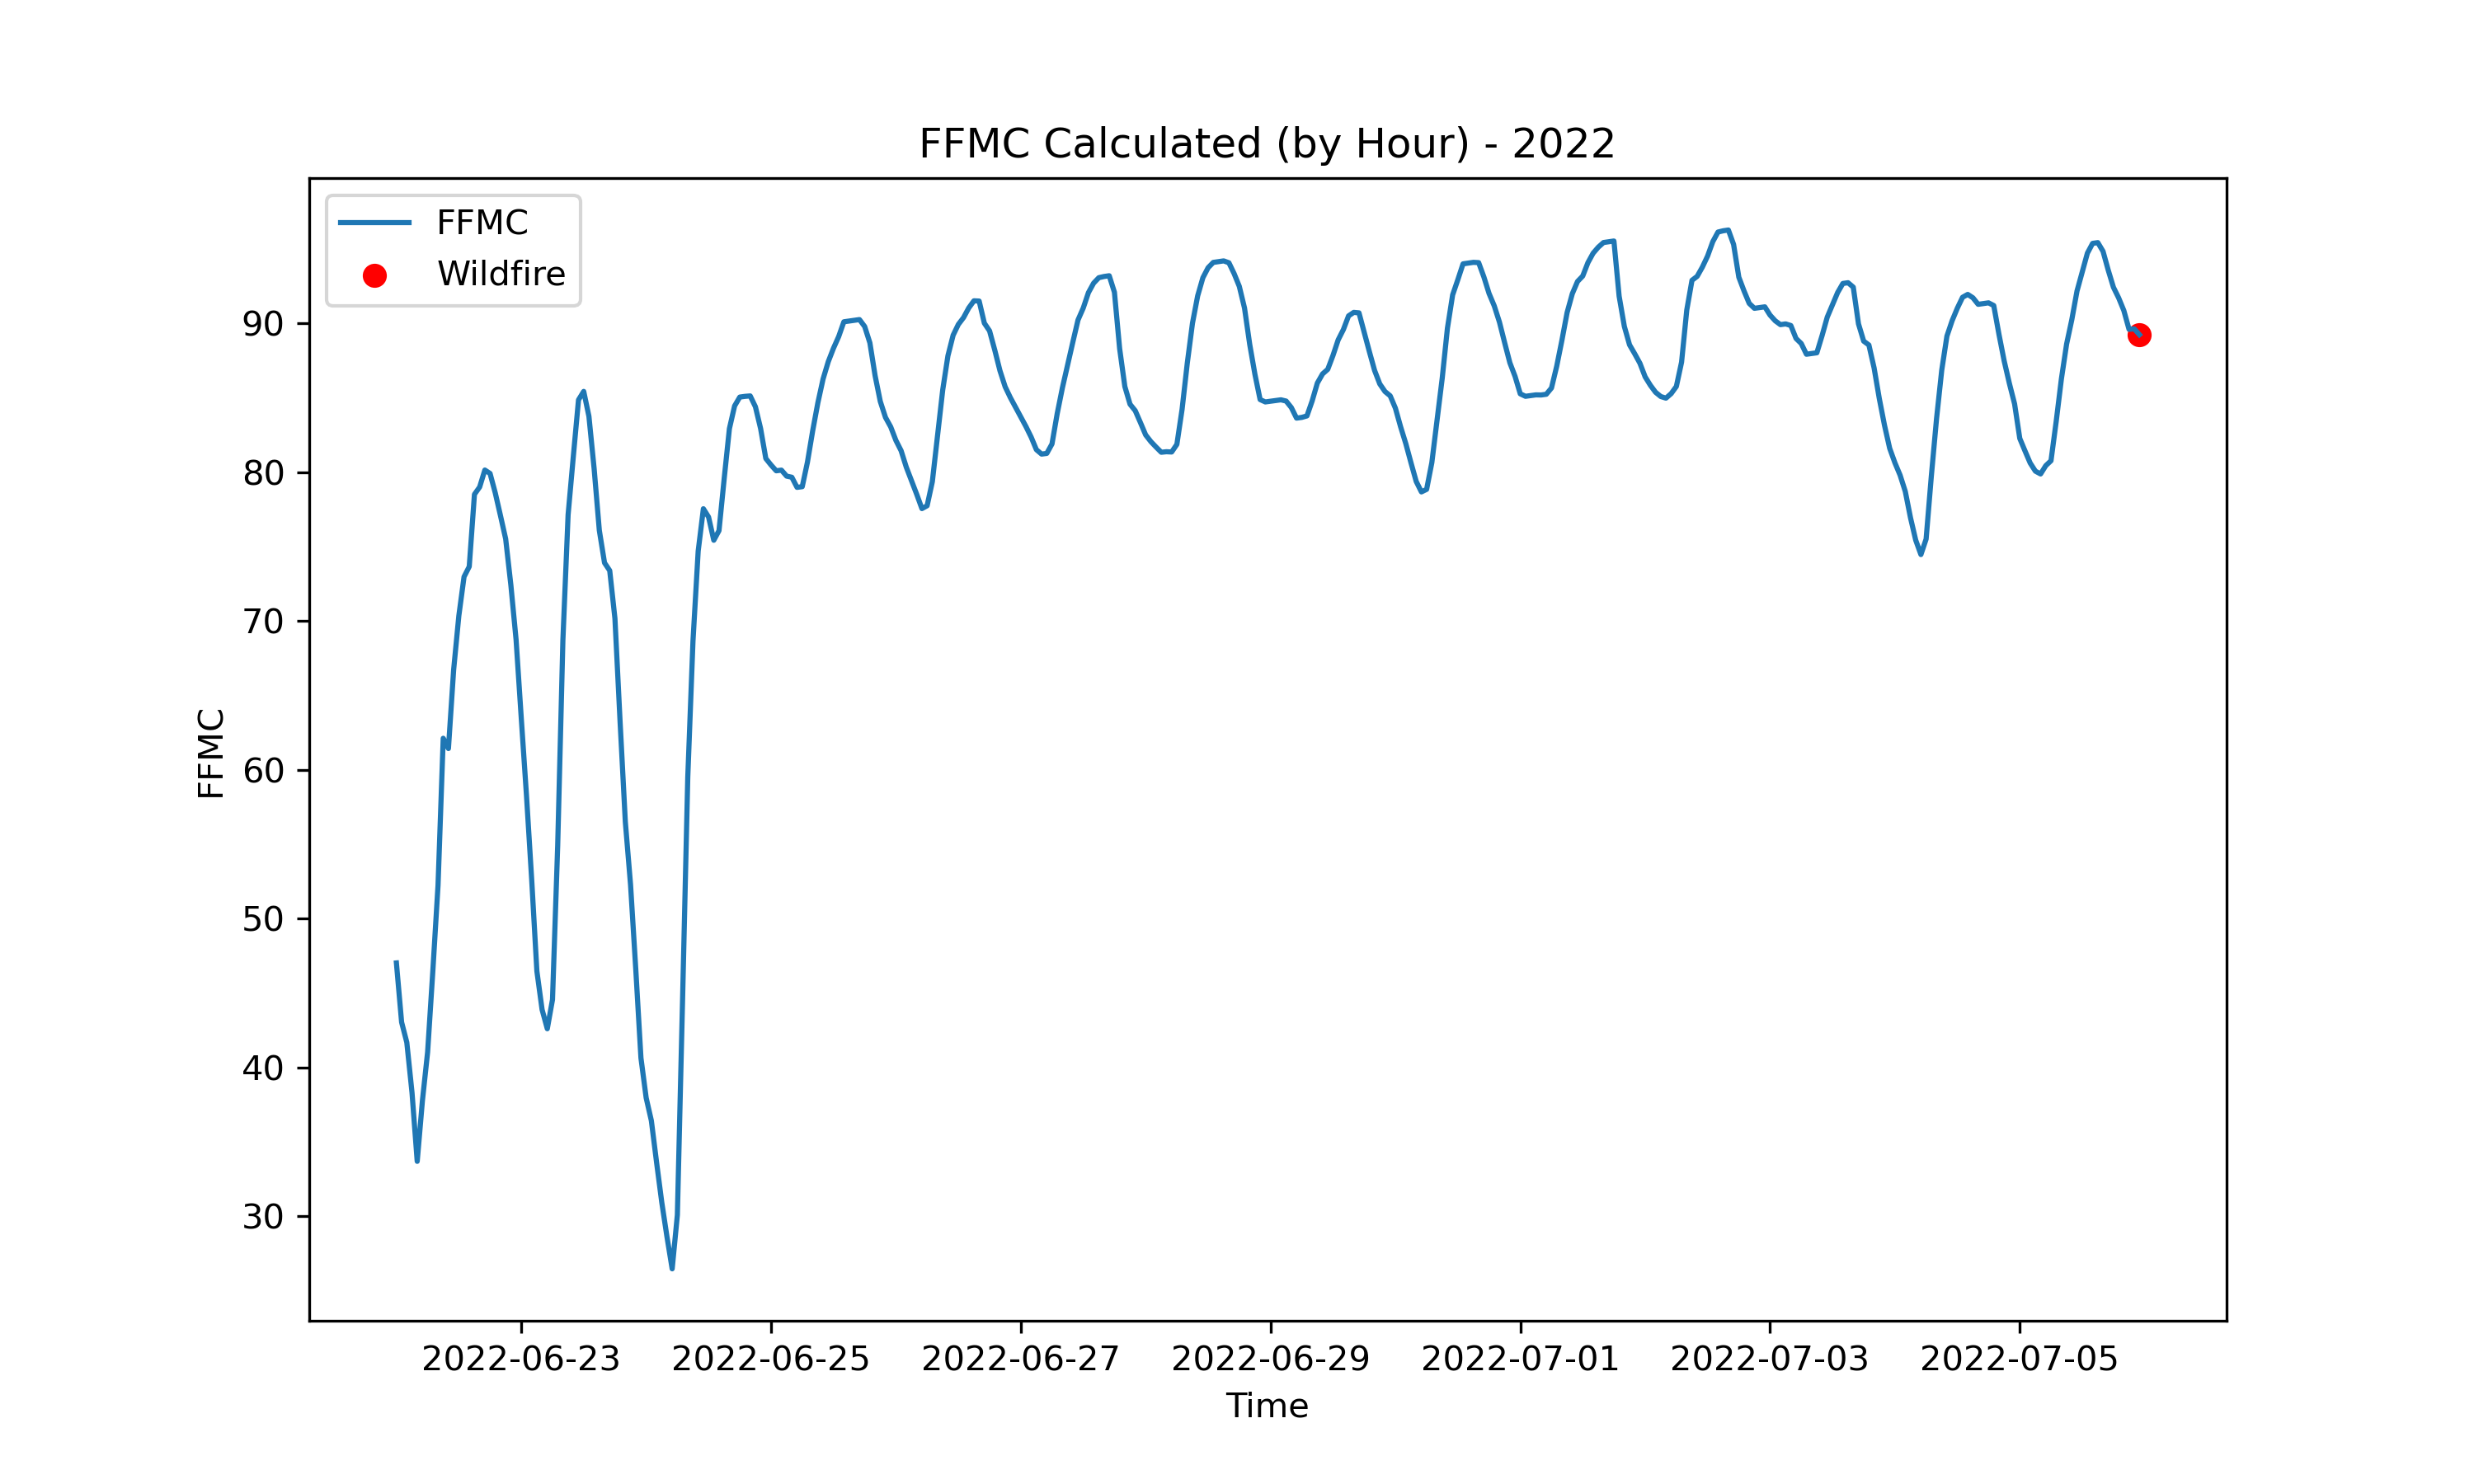
\includegraphics[width=\textwidth]{graphs/2022/2022CalcFFMC12.png}
		\caption{Caption for image 3}
		\label{fig:img3}
	\end{subfigure}
	
	\label{fig:all_images}
\end{figure}

\begin{figure}[h]
	\centering
	\caption{Caption for the whole figure}
	\begin{subfigure}{0.3\textwidth}
		\centering
		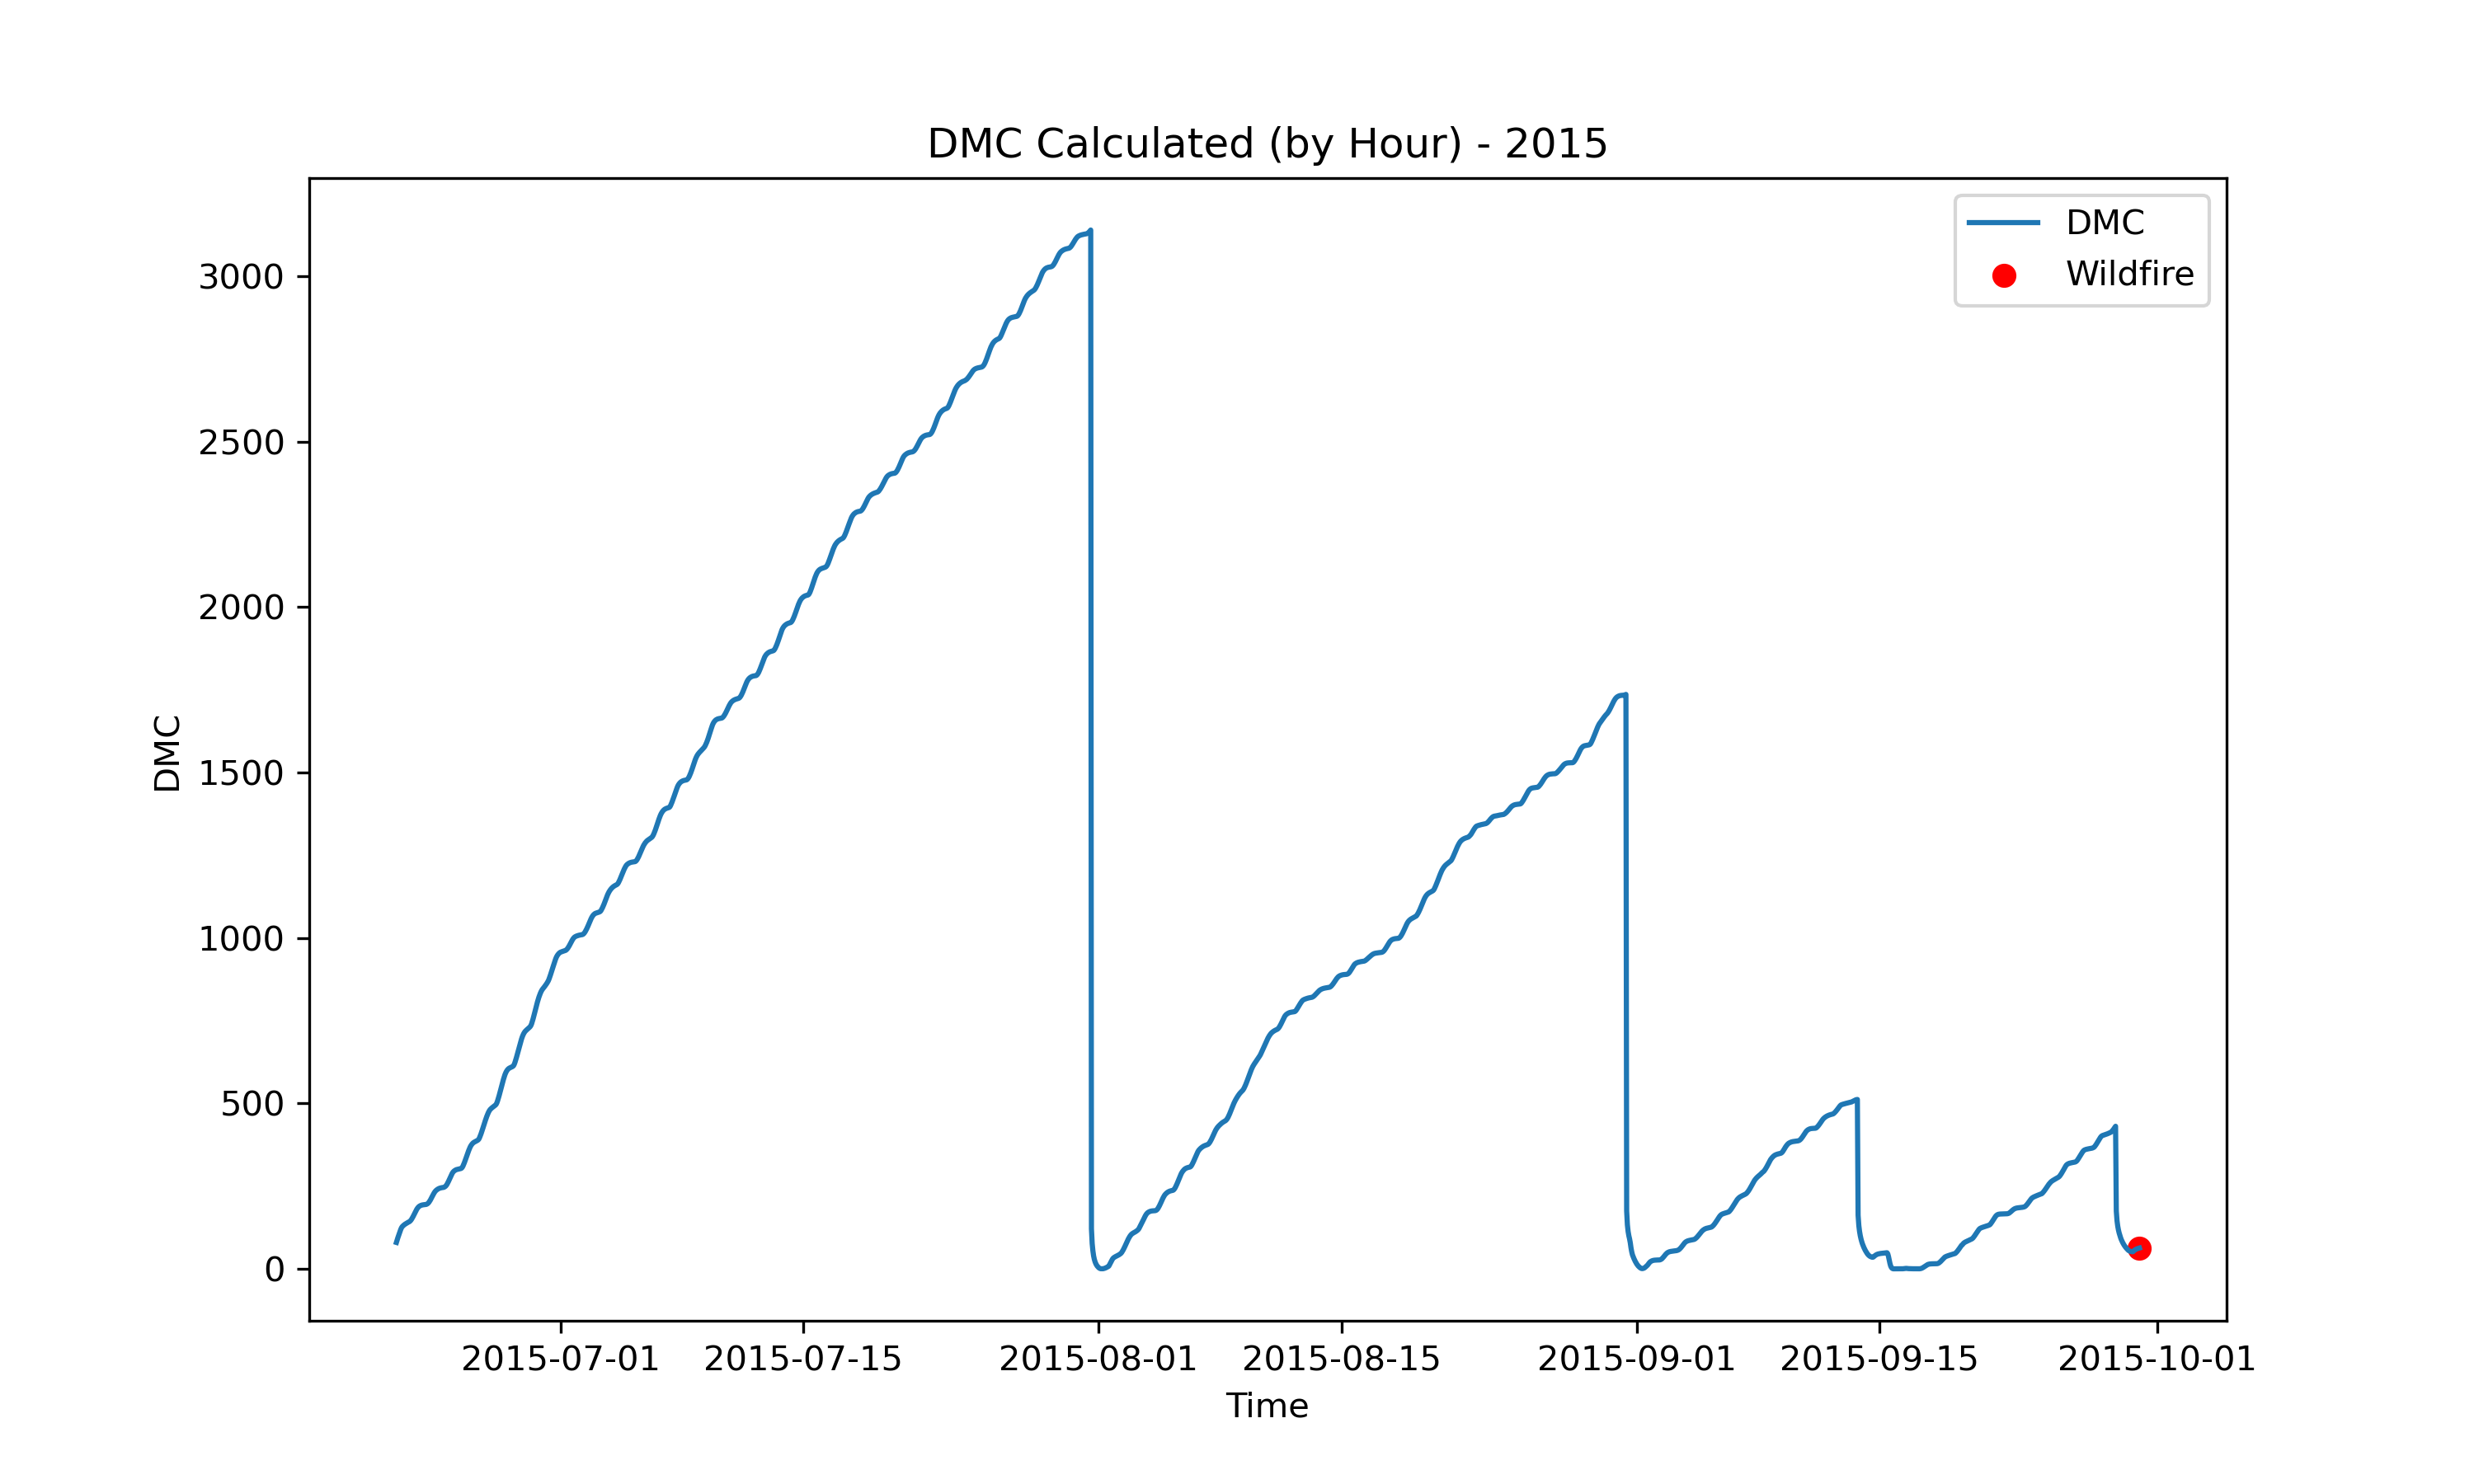
\includegraphics[width=\textwidth]{graphs/2015/byHour/2015CalcDMC12.png}
		\caption{Caption for image 1}
		\label{fig:img1}
	\end{subfigure}
	\hfill
	\begin{subfigure}{0.3\textwidth}
		\centering
		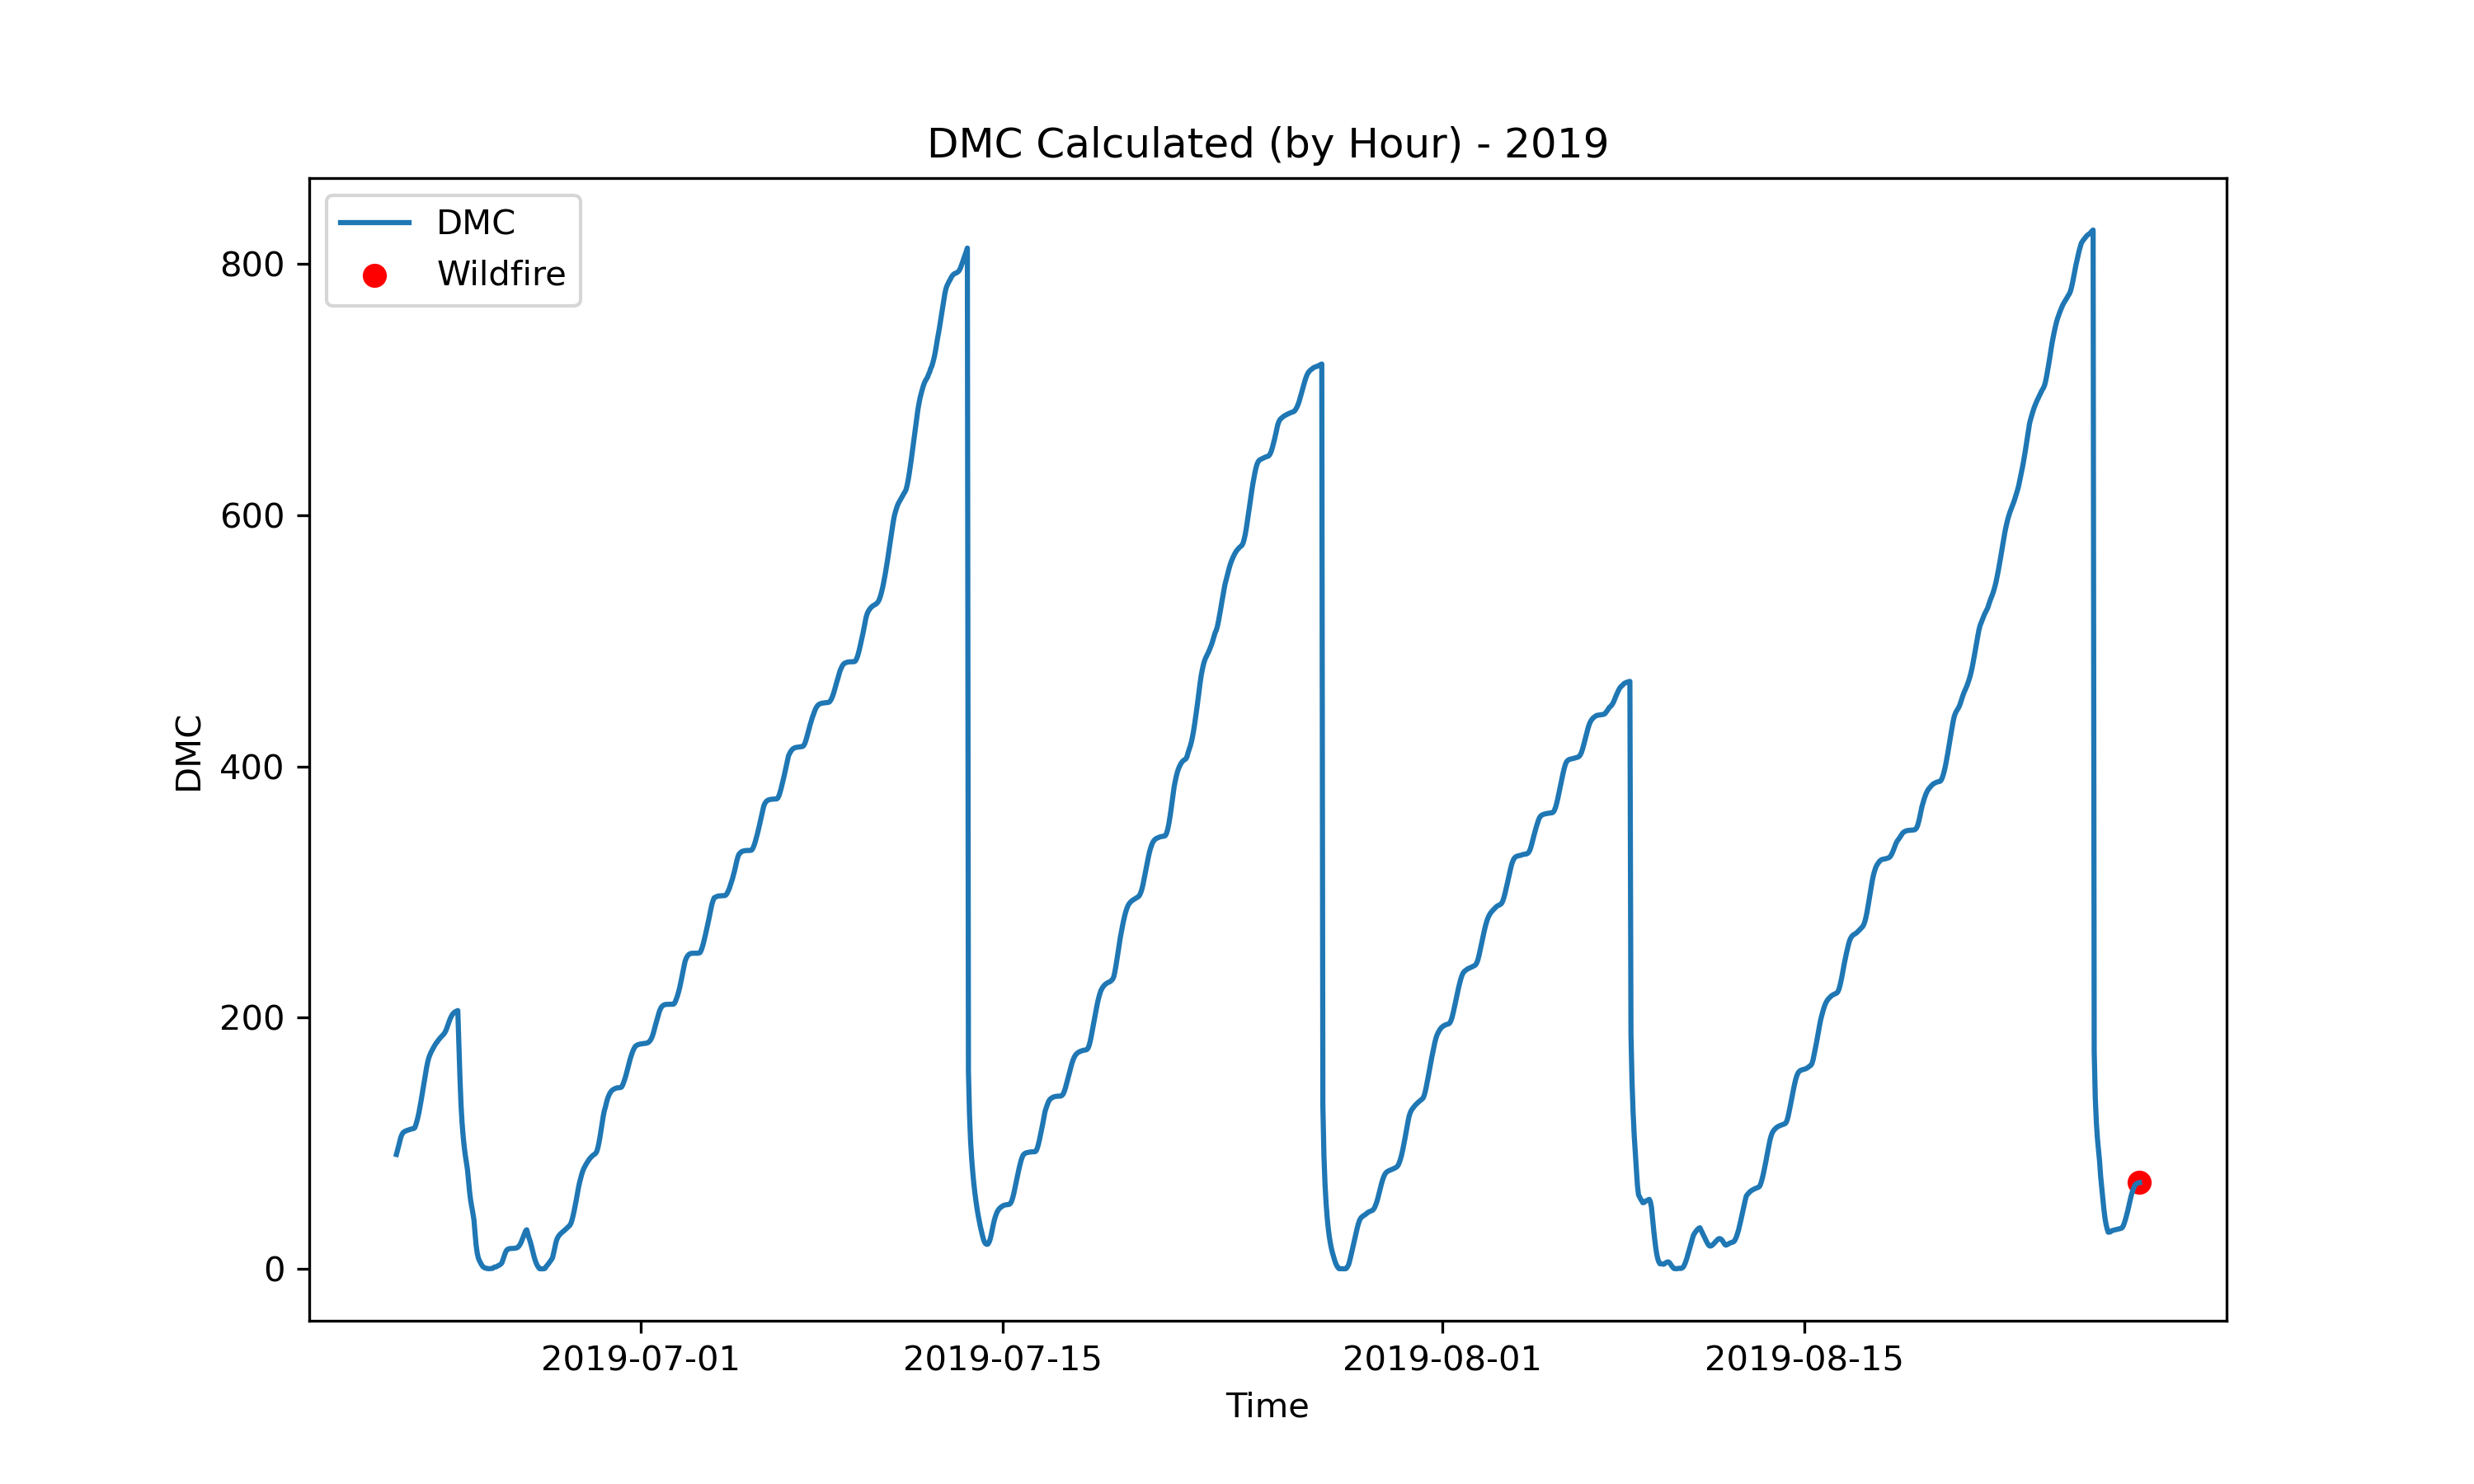
\includegraphics[width=\textwidth]{graphs/2019/byHour/2019CalcDMC12.png}
		\caption{Caption for image 2}
		\label{fig:img2}
	\end{subfigure}
	\hfill
	\begin{subfigure}{0.3\textwidth}
		\centering
		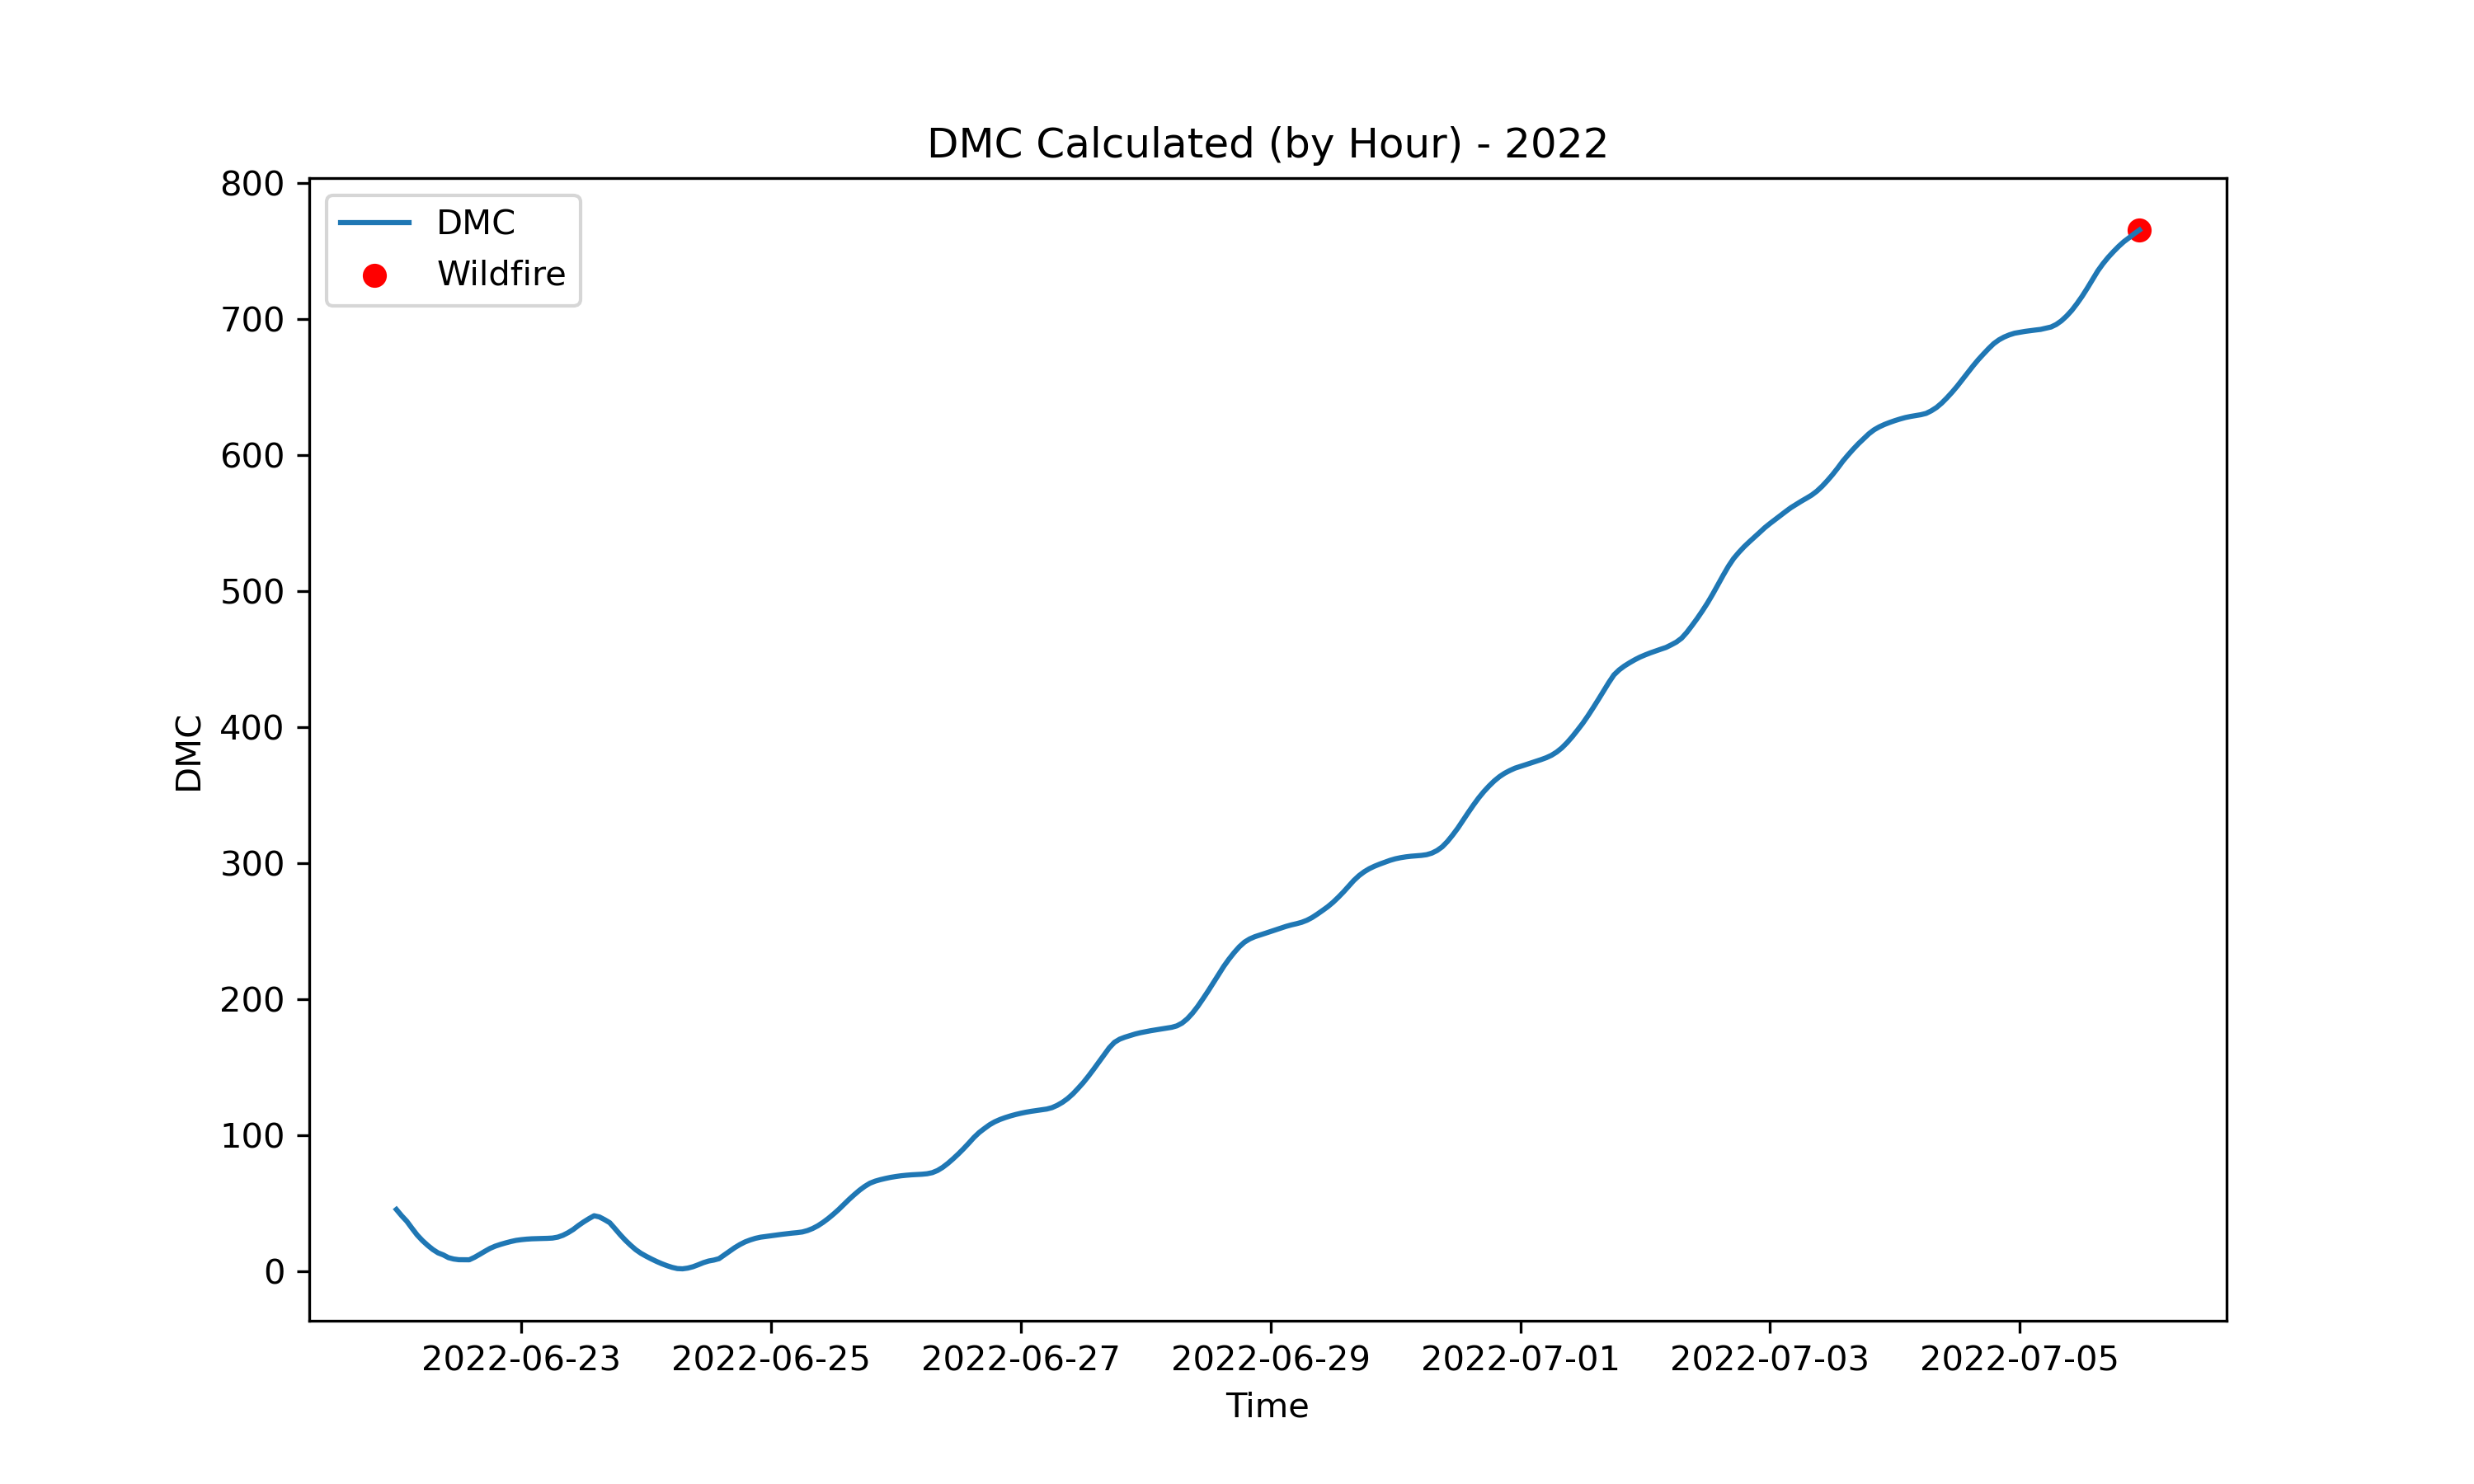
\includegraphics[width=\textwidth]{graphs/2022/2022CalcDMC12.png}
		\caption{Caption for image 3}
		\label{fig:img3}
	\end{subfigure}
	
	\label{fig:all_images}
\end{figure}

\begin{figure}[h]
	\centering
	\caption{Caption for the whole figure}
	\begin{subfigure}{0.3\textwidth}
		\centering
		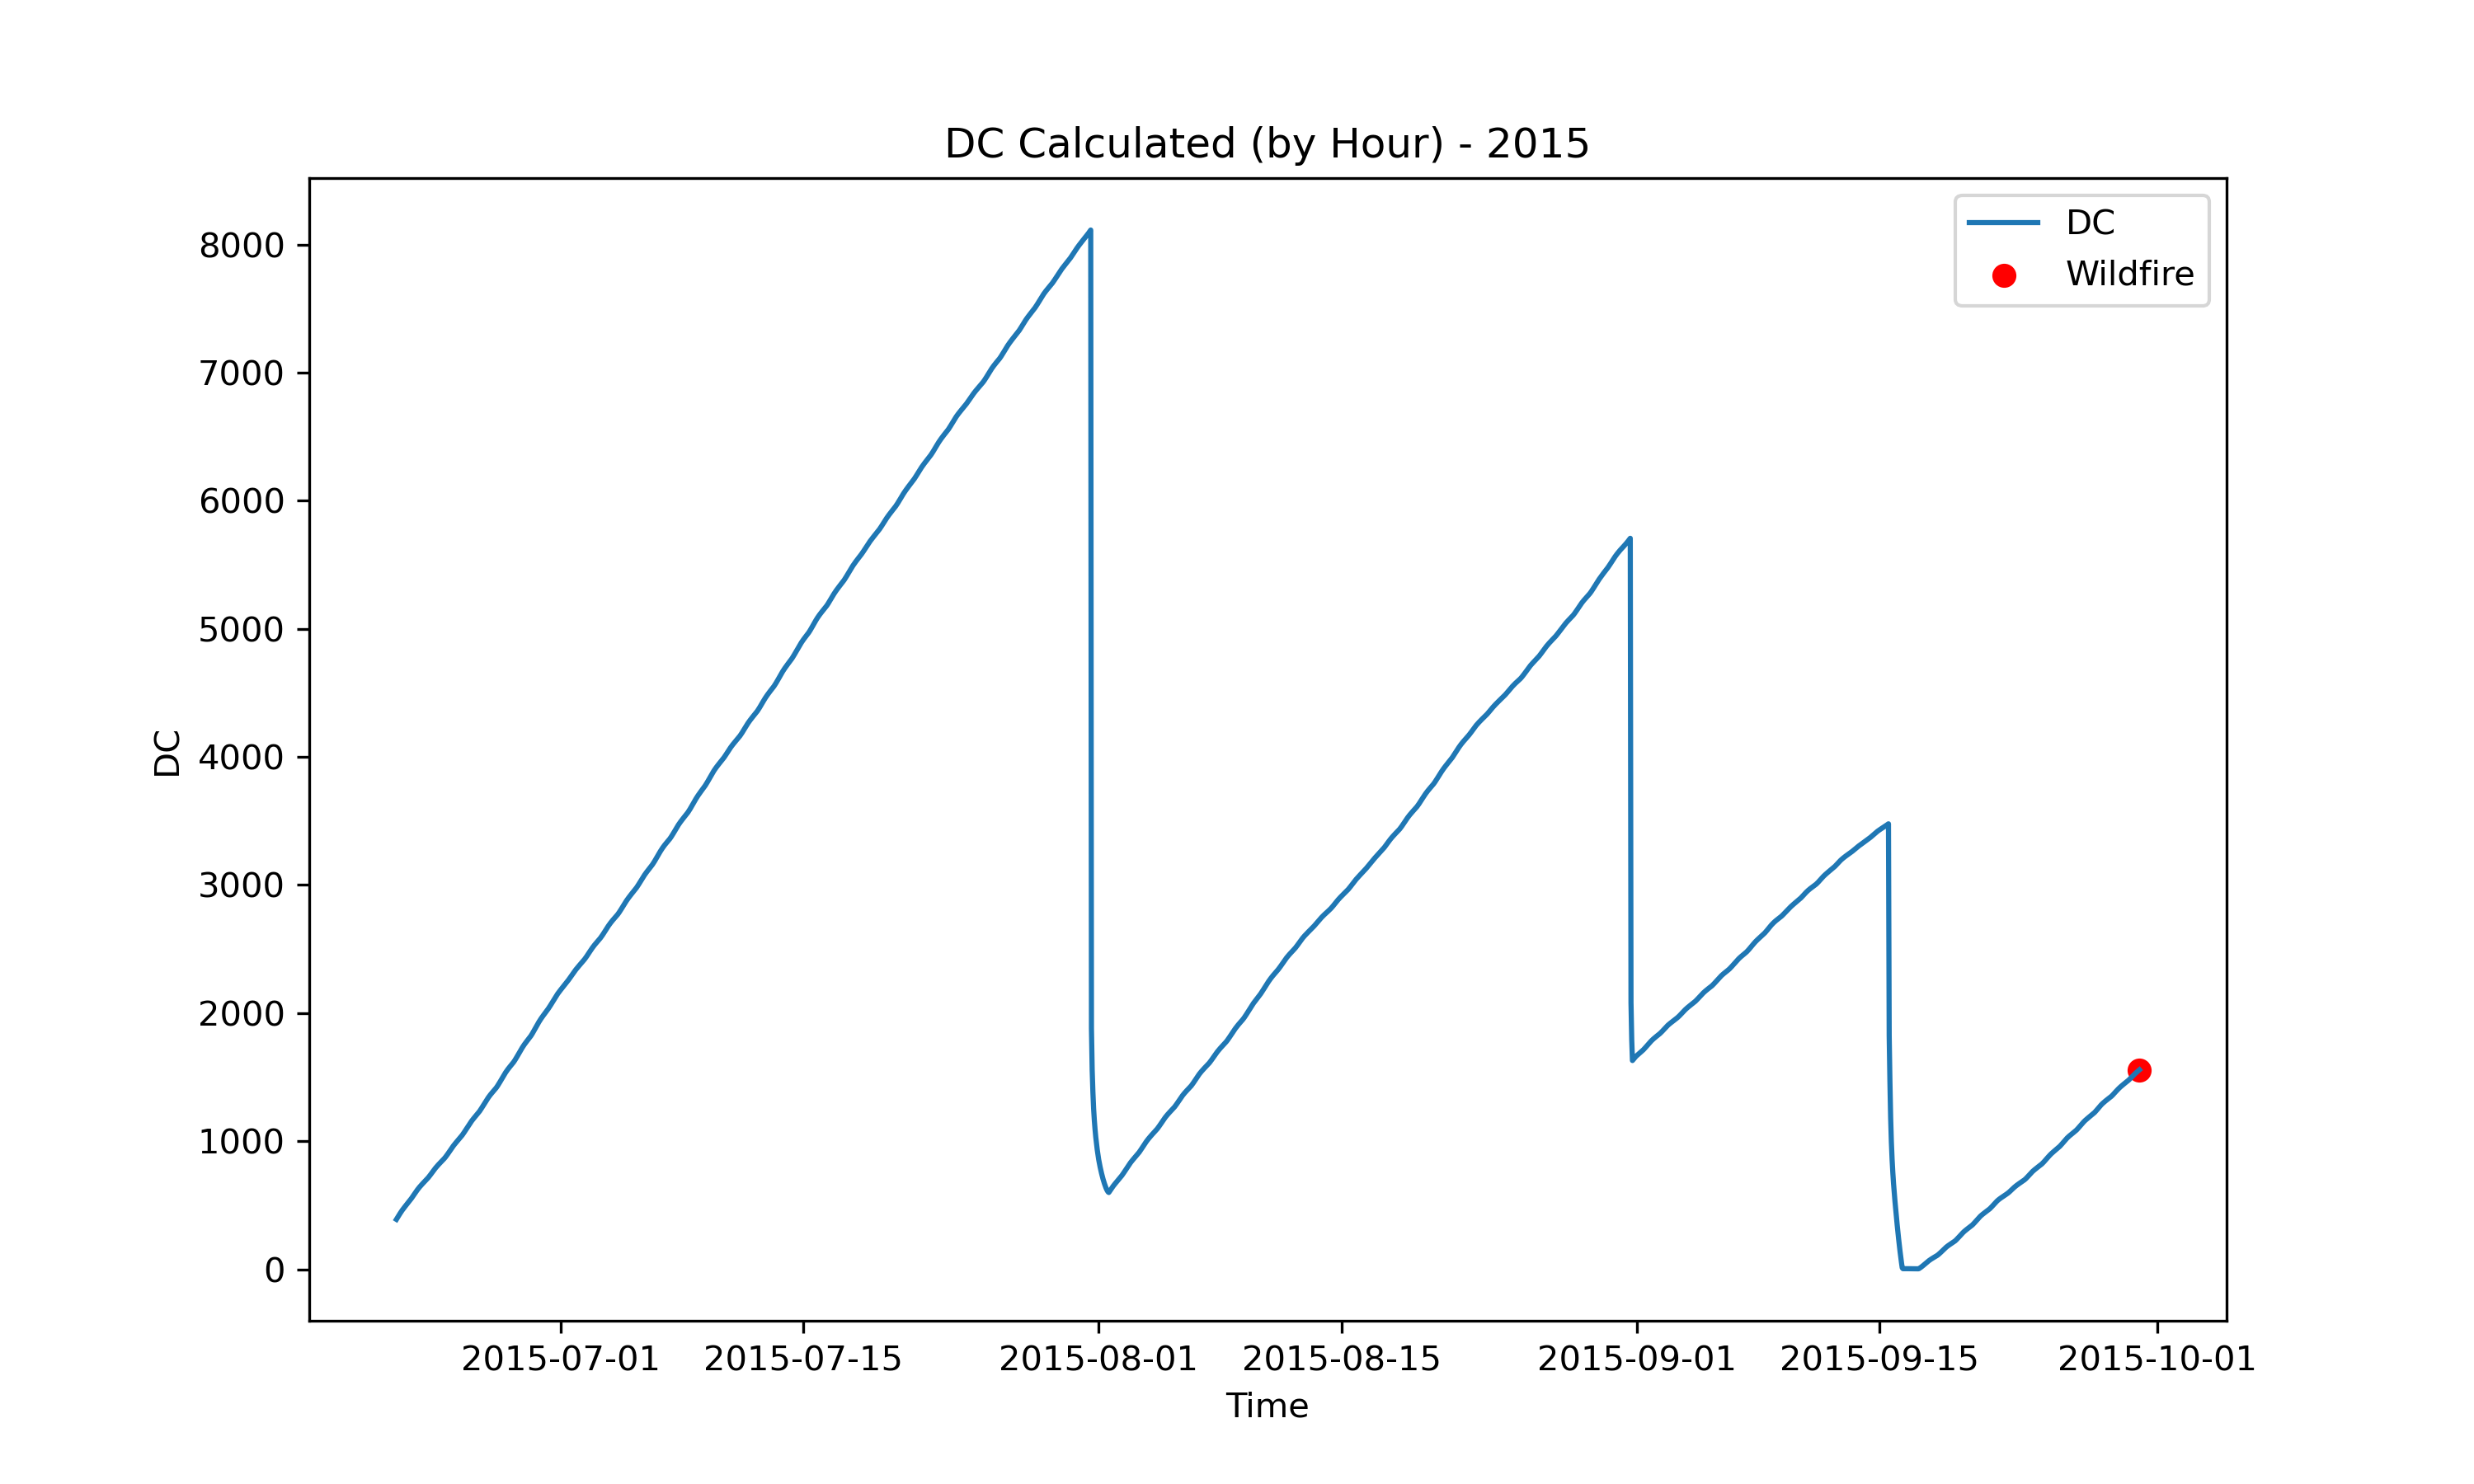
\includegraphics[width=\textwidth]{graphs/2015/byHour/2015CalcDC12.png}
		\caption{Caption for image 1}
		\label{fig:img1}
	\end{subfigure}
	\hfill
	\begin{subfigure}{0.3\textwidth}
		\centering
		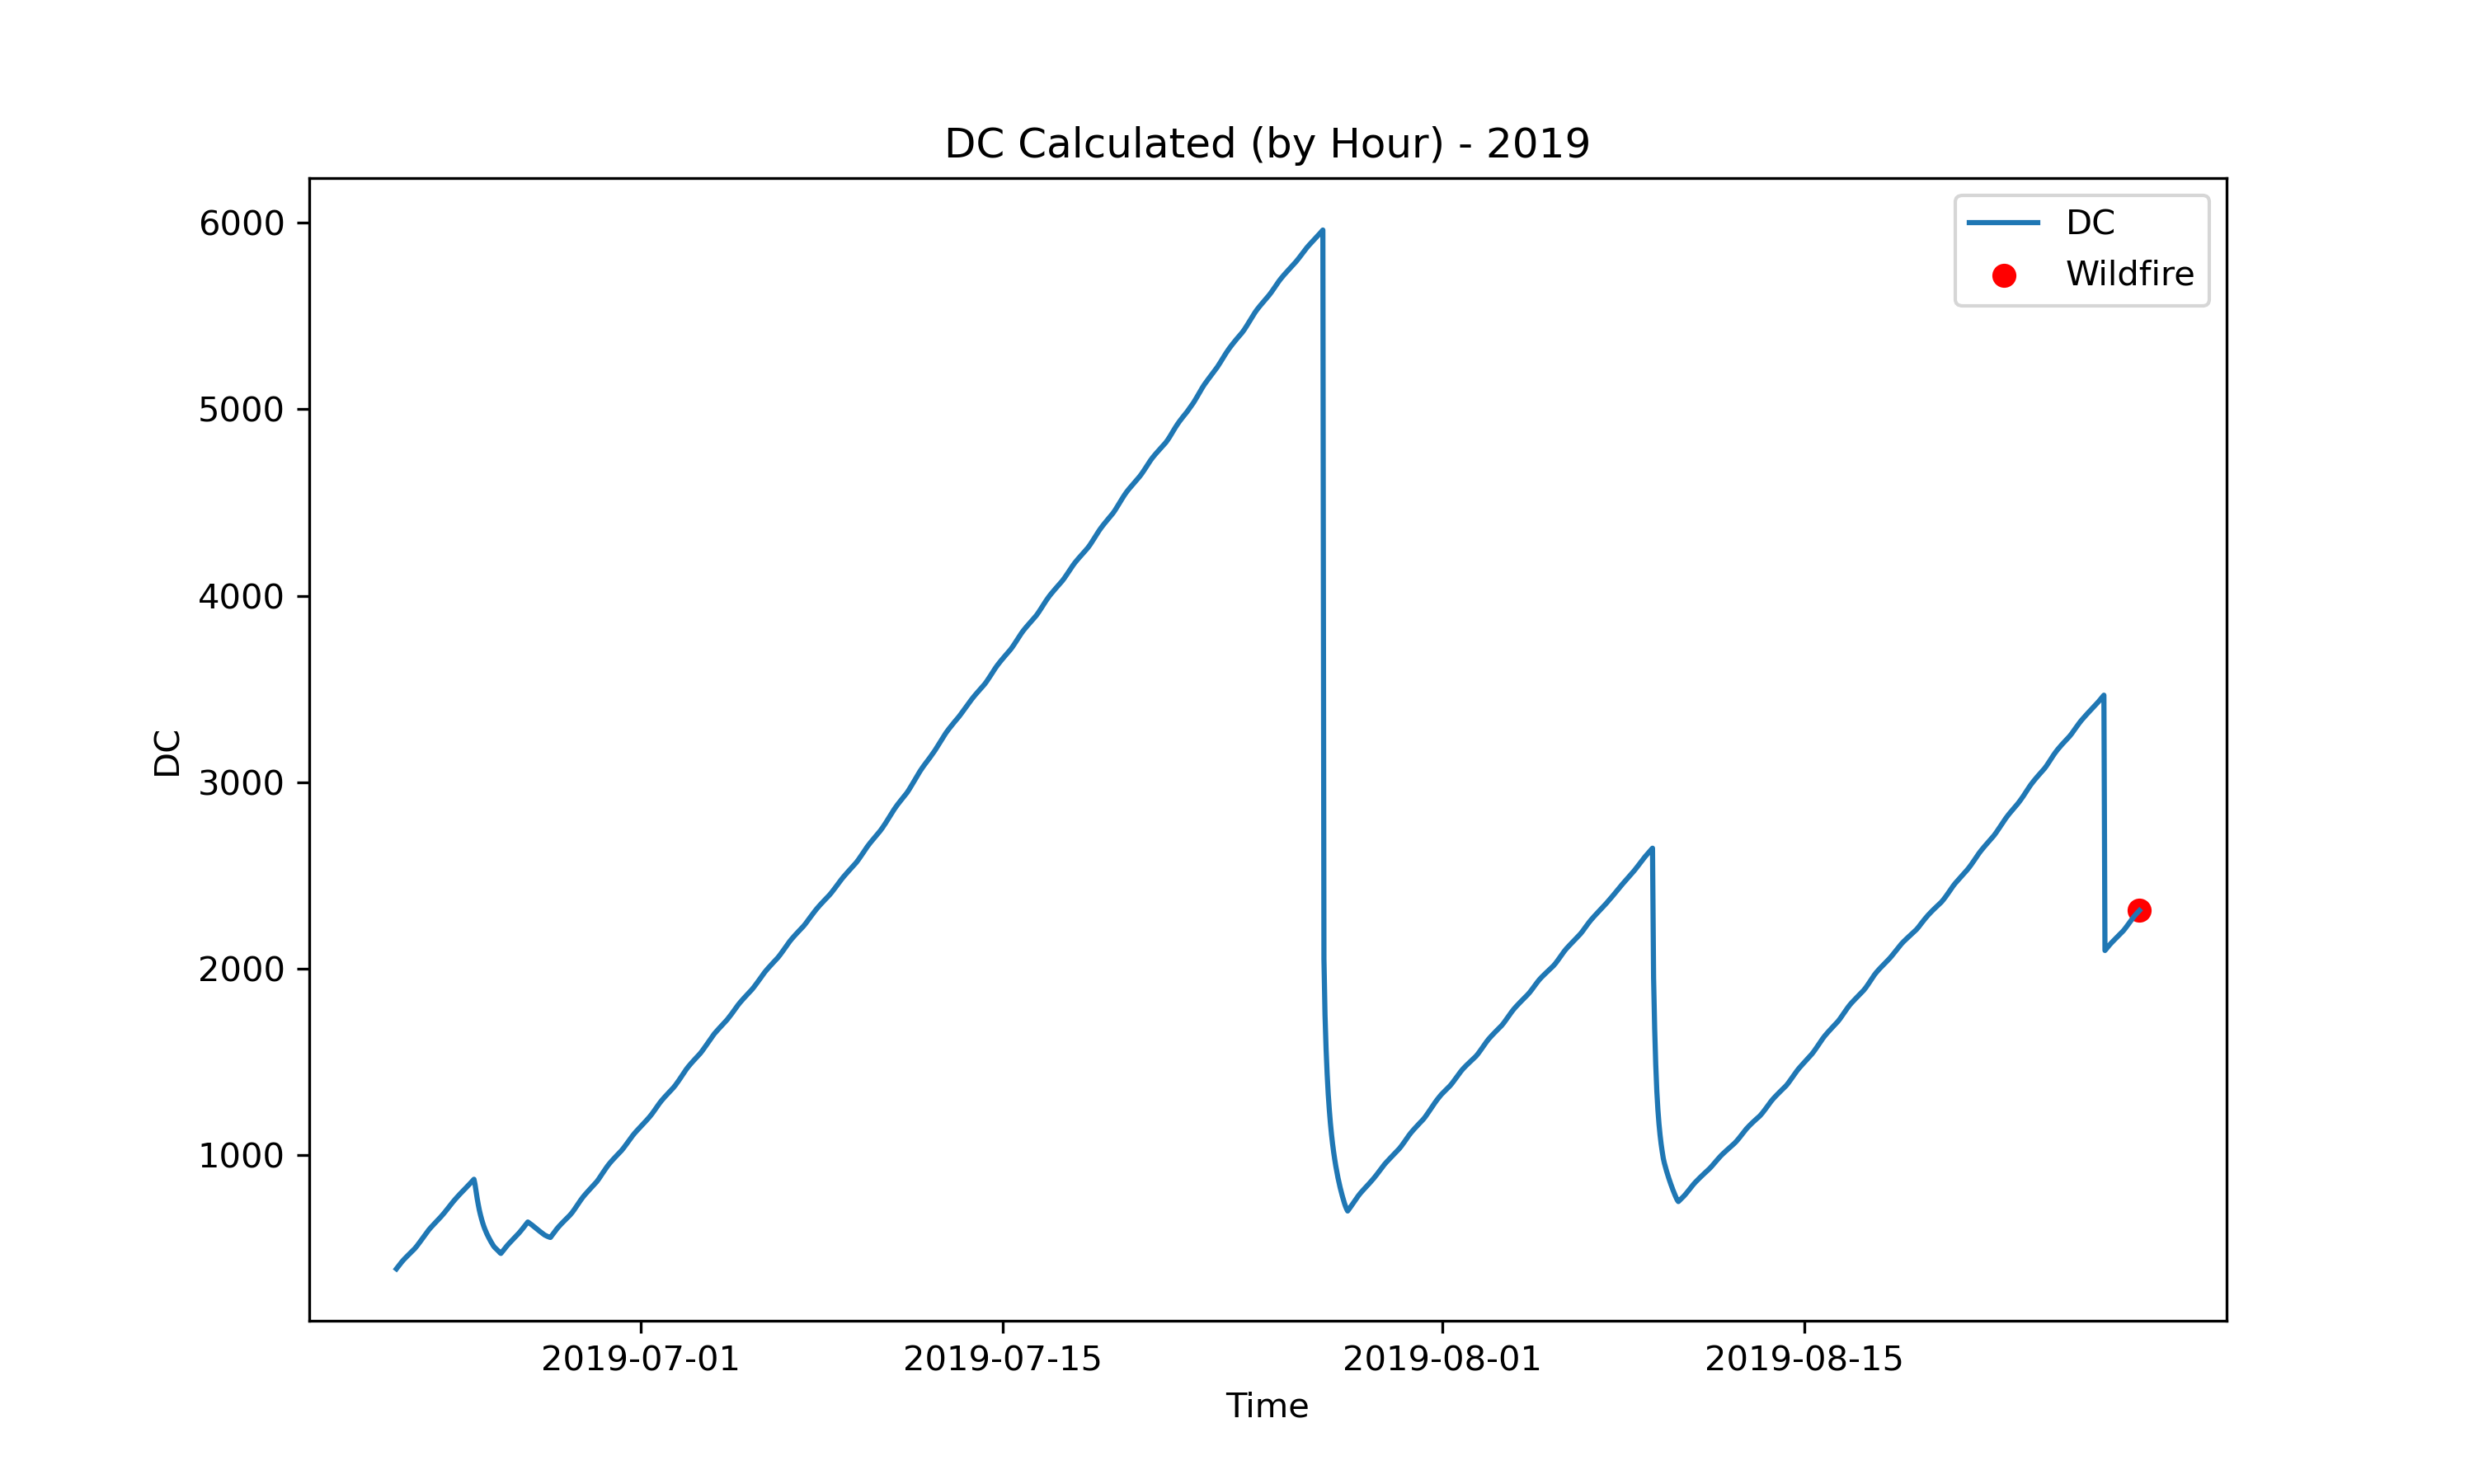
\includegraphics[width=\textwidth]{graphs/2019/byHour/2019CalcDC12.png}
		\caption{Caption for image 2}
		\label{fig:img2}
	\end{subfigure}
	\hfill
	\begin{subfigure}{0.3\textwidth}
		\centering
		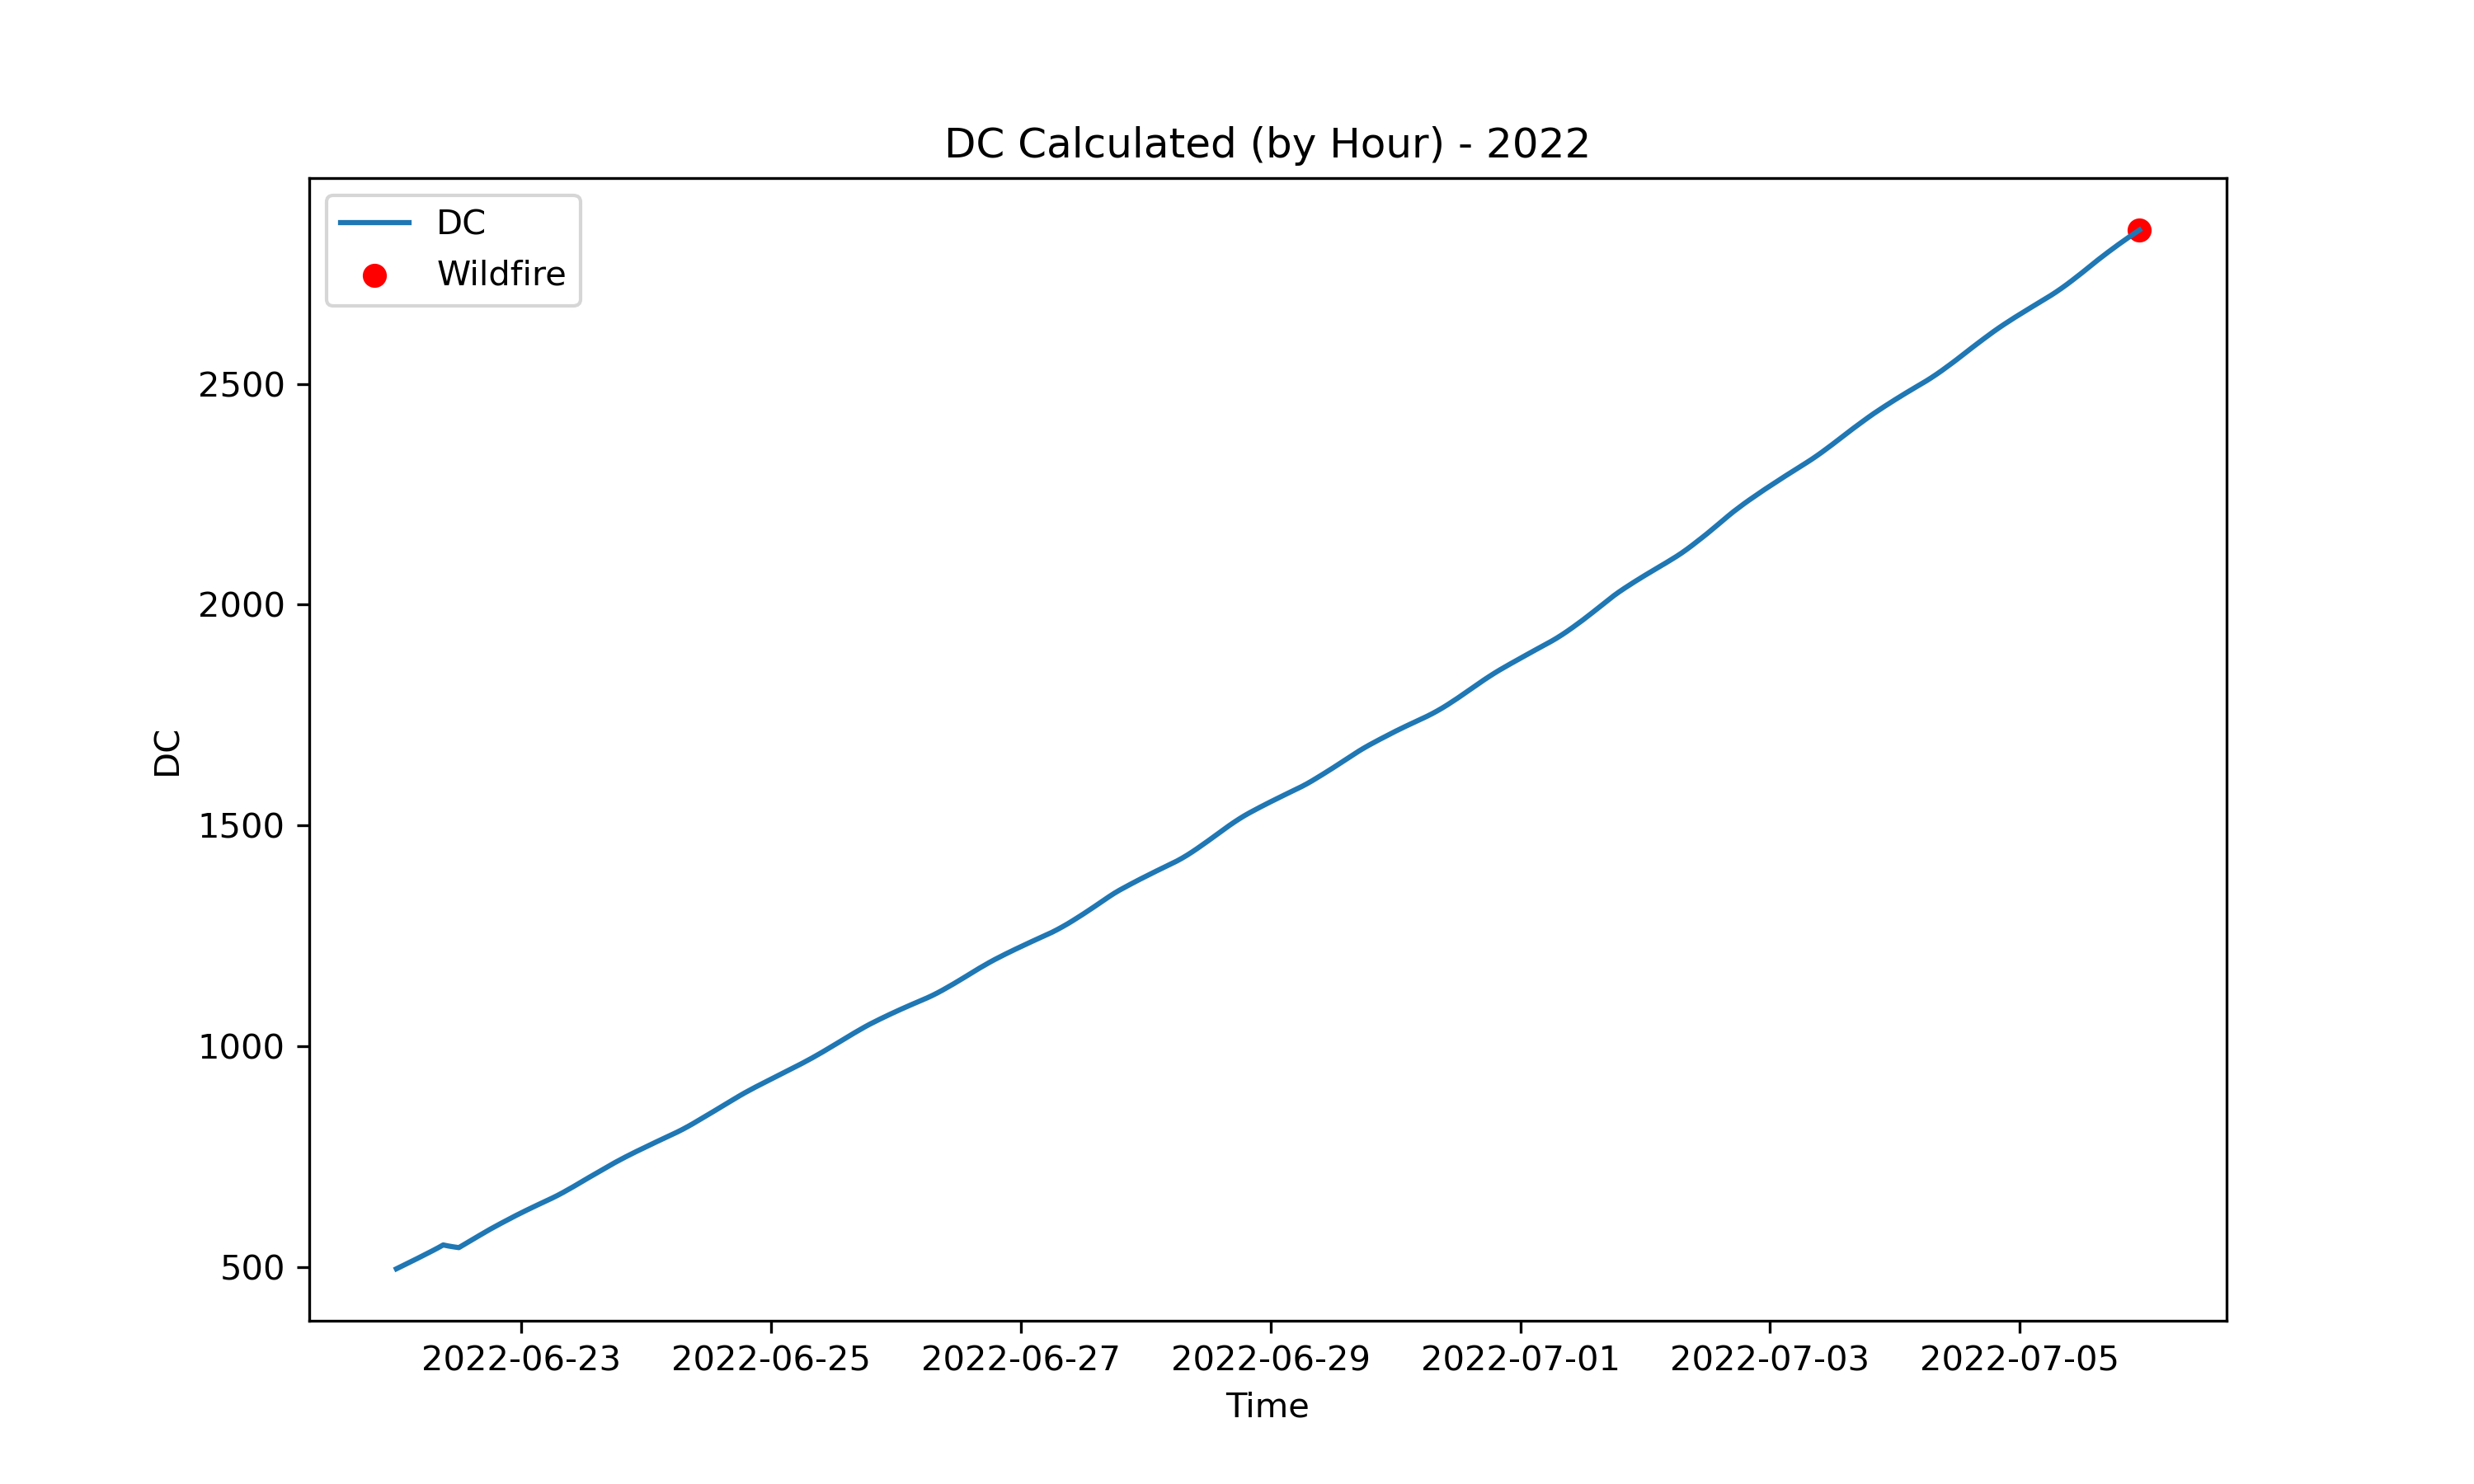
\includegraphics[width=\textwidth]{graphs/2022/2022CalcDC12.png}
		\caption{Caption for image 3}
		\label{fig:img3}
	\end{subfigure}
	
	\label{fig:all_images}
\end{figure}

\begin{figure}[h]
	\centering
	\caption{Caption for the whole figure}
	\begin{subfigure}{0.3\textwidth}
		\centering
		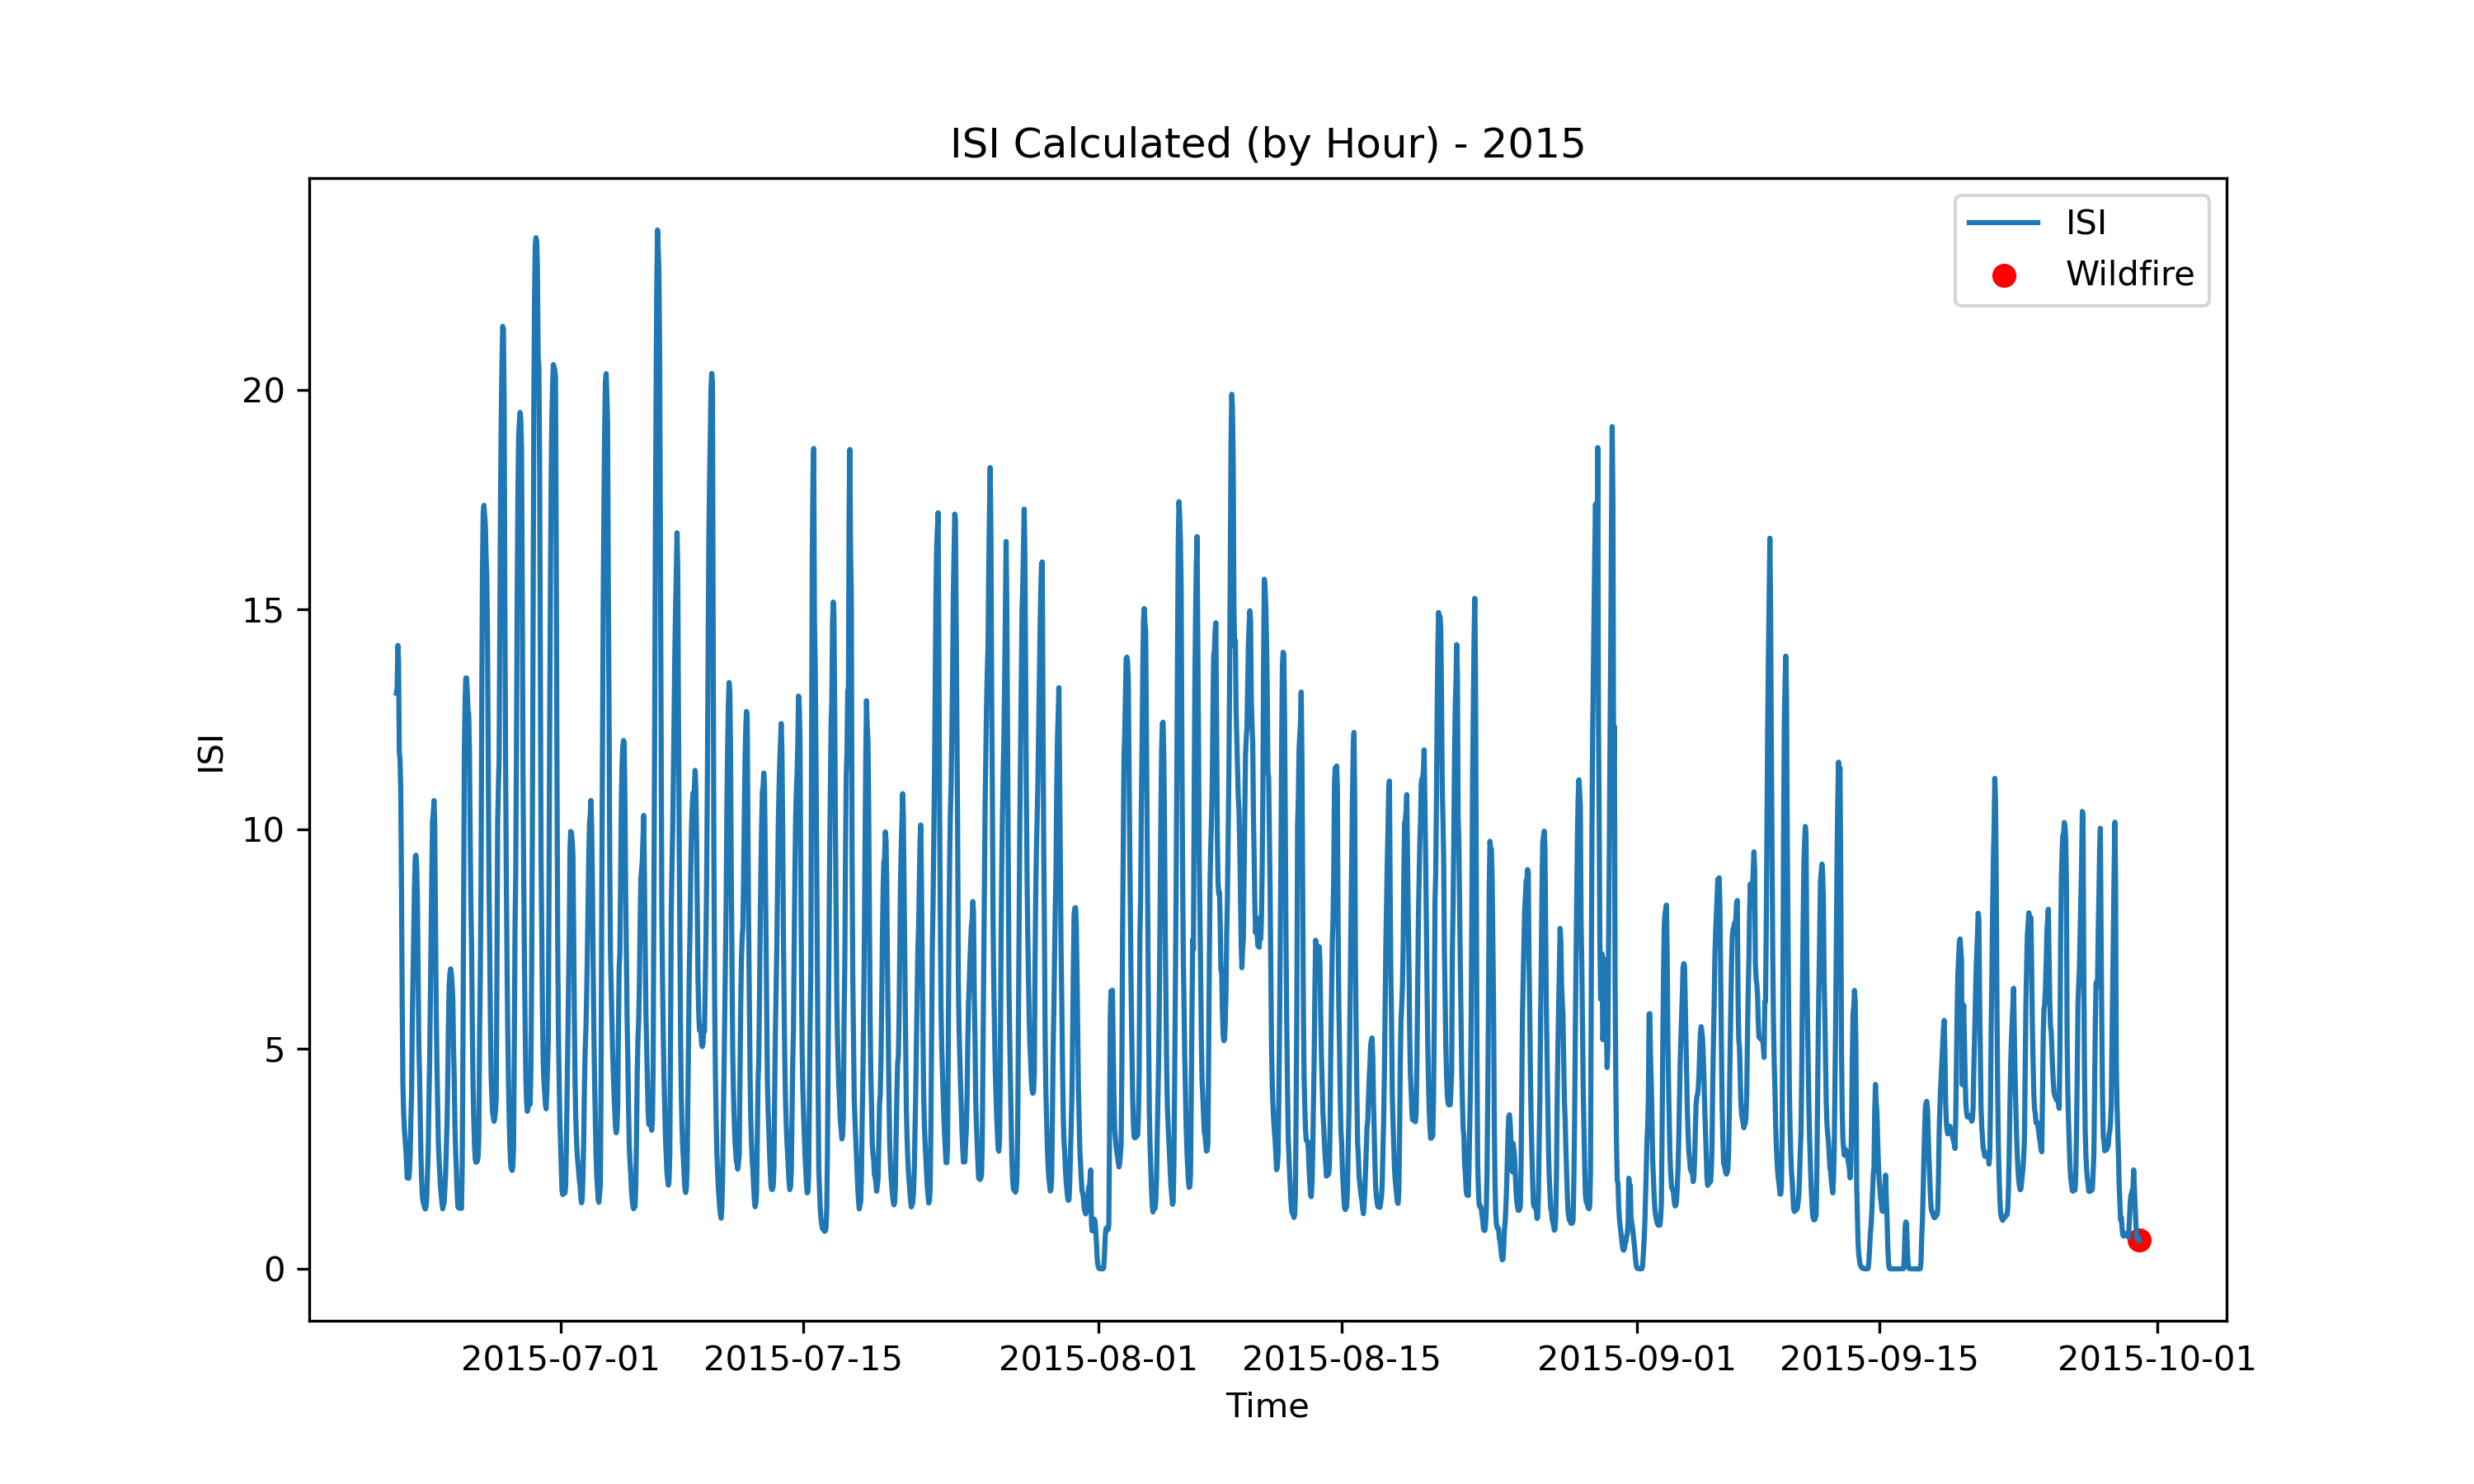
\includegraphics[width=\textwidth]{graphs/2015/byHour/2015CalcISI12.png}
		\caption{Caption for image 1}
		\label{fig:img1}
	\end{subfigure}
	\hfill
	\begin{subfigure}{0.3\textwidth}
		\centering
		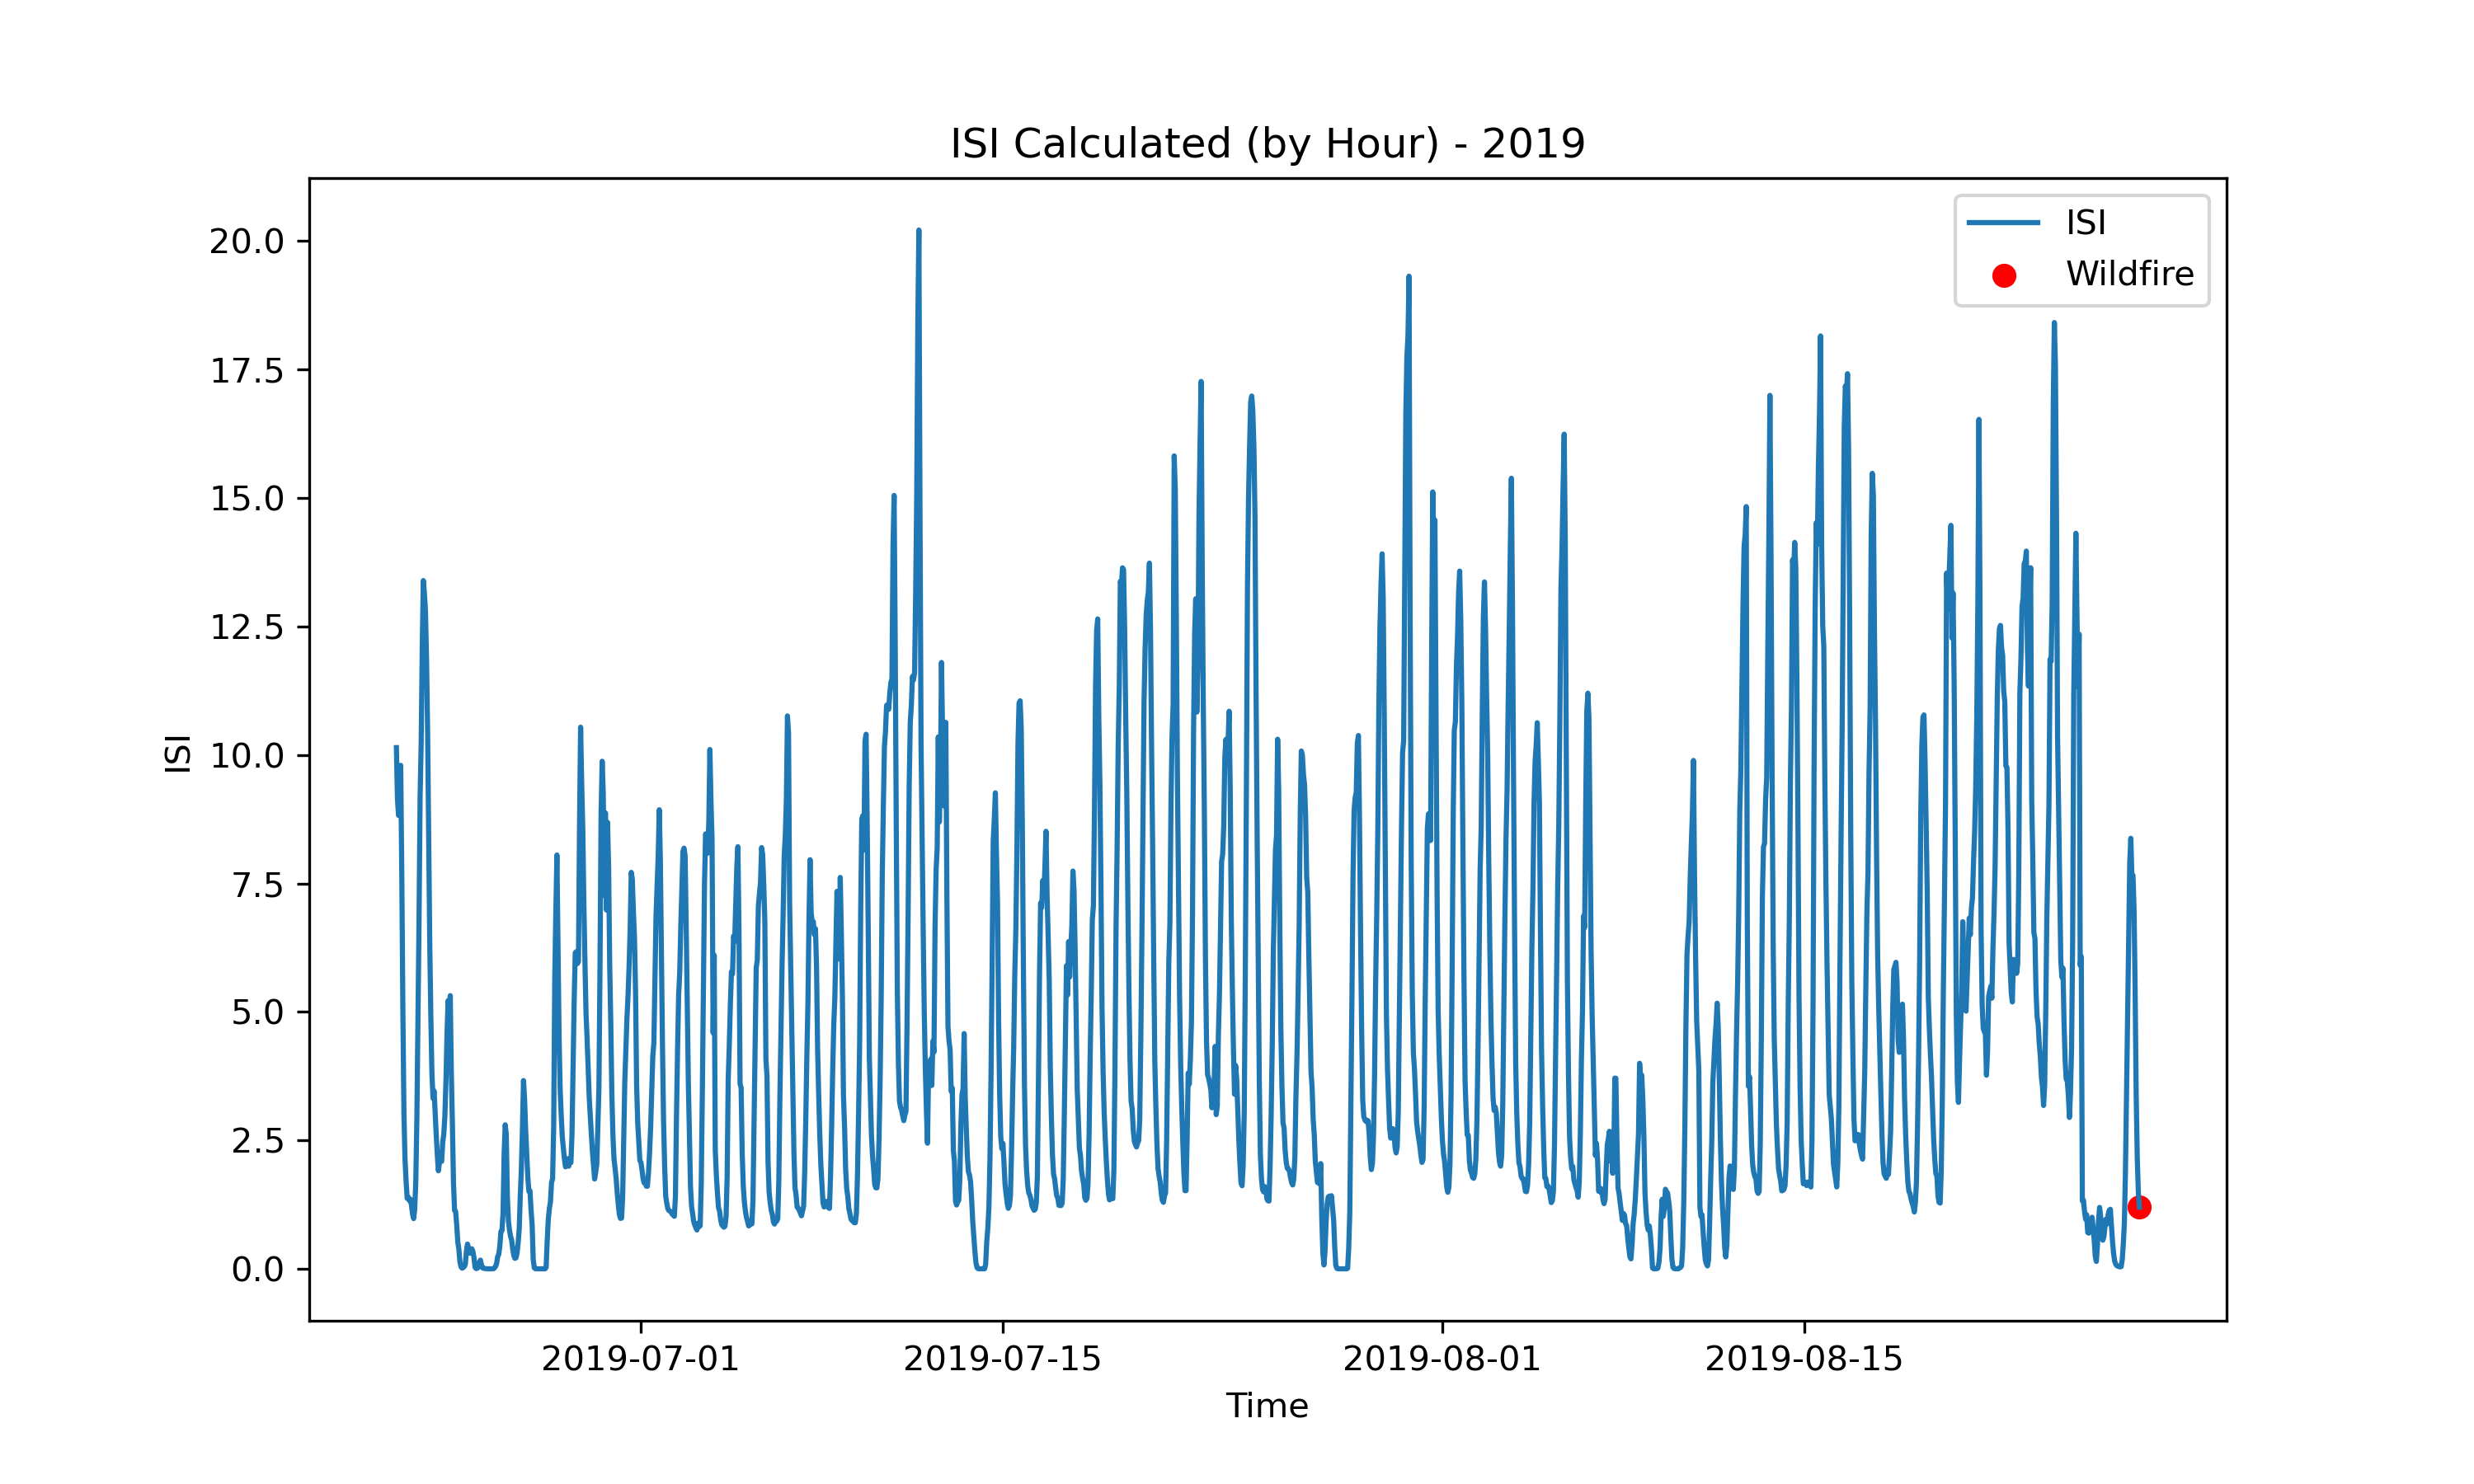
\includegraphics[width=\textwidth]{graphs/2019/byHour/2019CalcISI12.png}
		\caption{Caption for image 2}
		\label{fig:img2}
	\end{subfigure}
	\hfill
	\begin{subfigure}{0.3\textwidth}
		\centering
		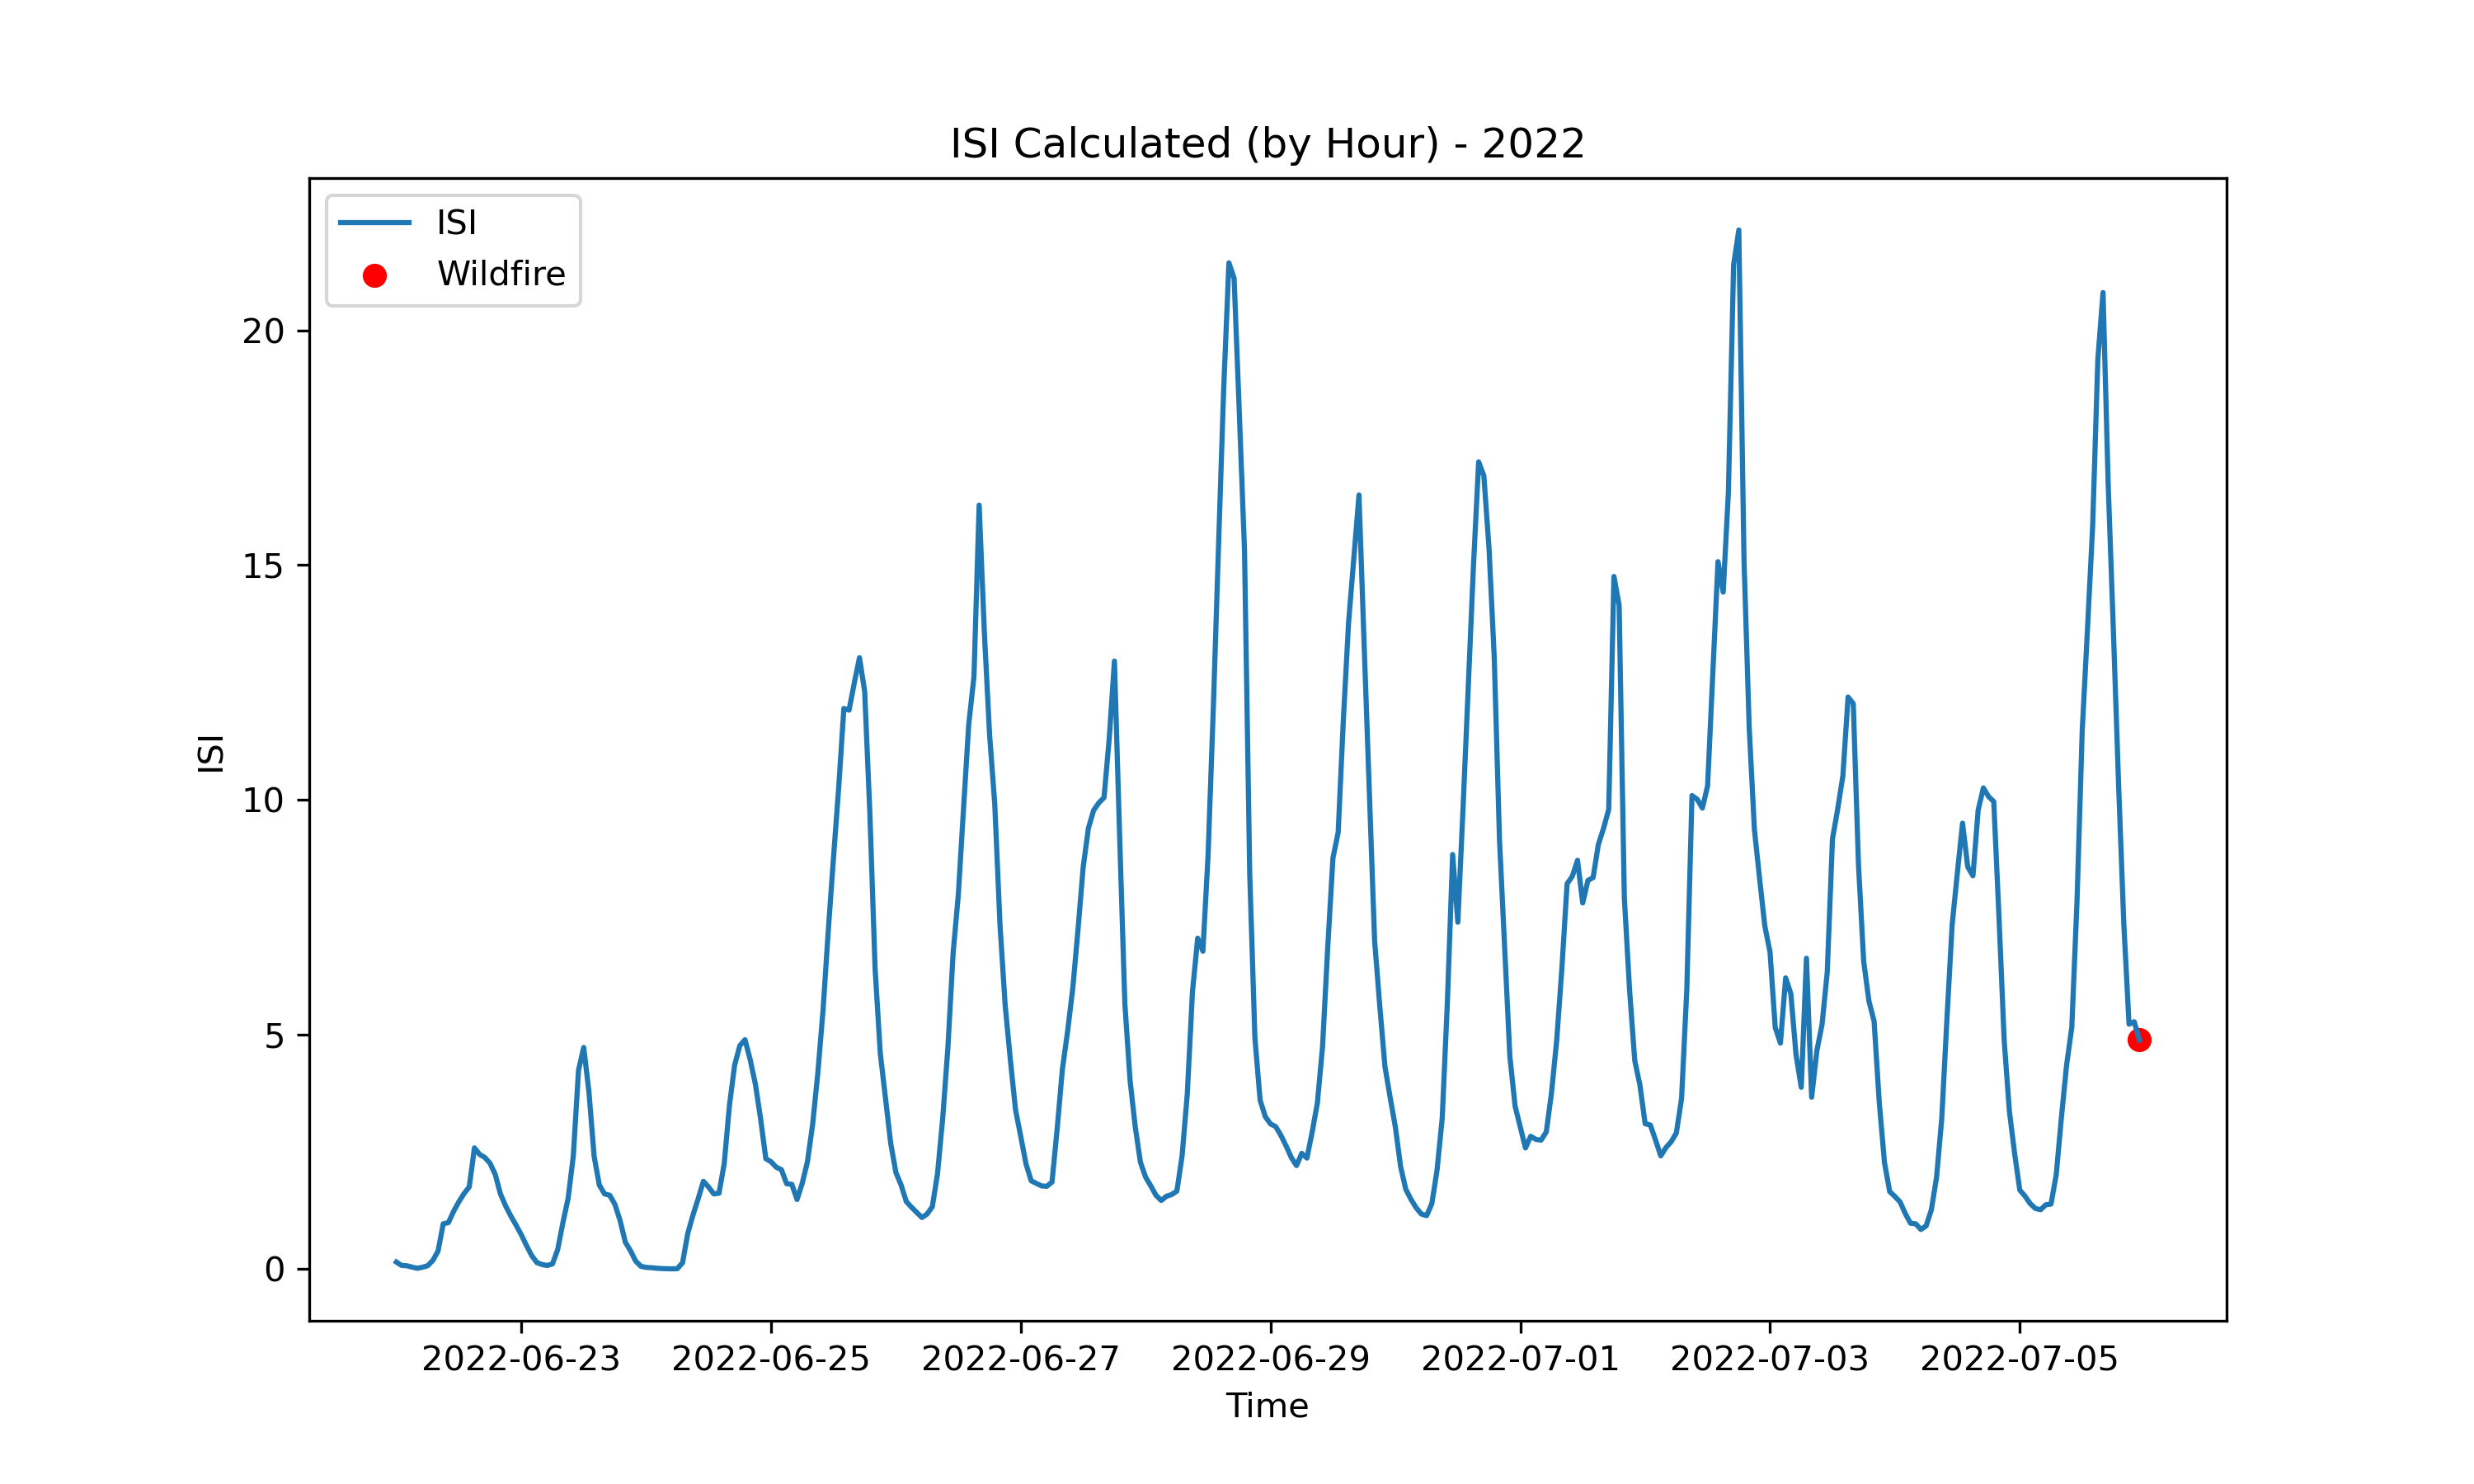
\includegraphics[width=\textwidth]{graphs/2022/2022CalcISI12.png}
		\caption{Caption for image 3}
		\label{fig:img3}
	\end{subfigure}
	
	\label{fig:all_images}
\end{figure}

\begin{figure}[h]
	\centering
	\caption{Caption for the whole figure}
	\begin{subfigure}{0.3\textwidth}
		\centering
		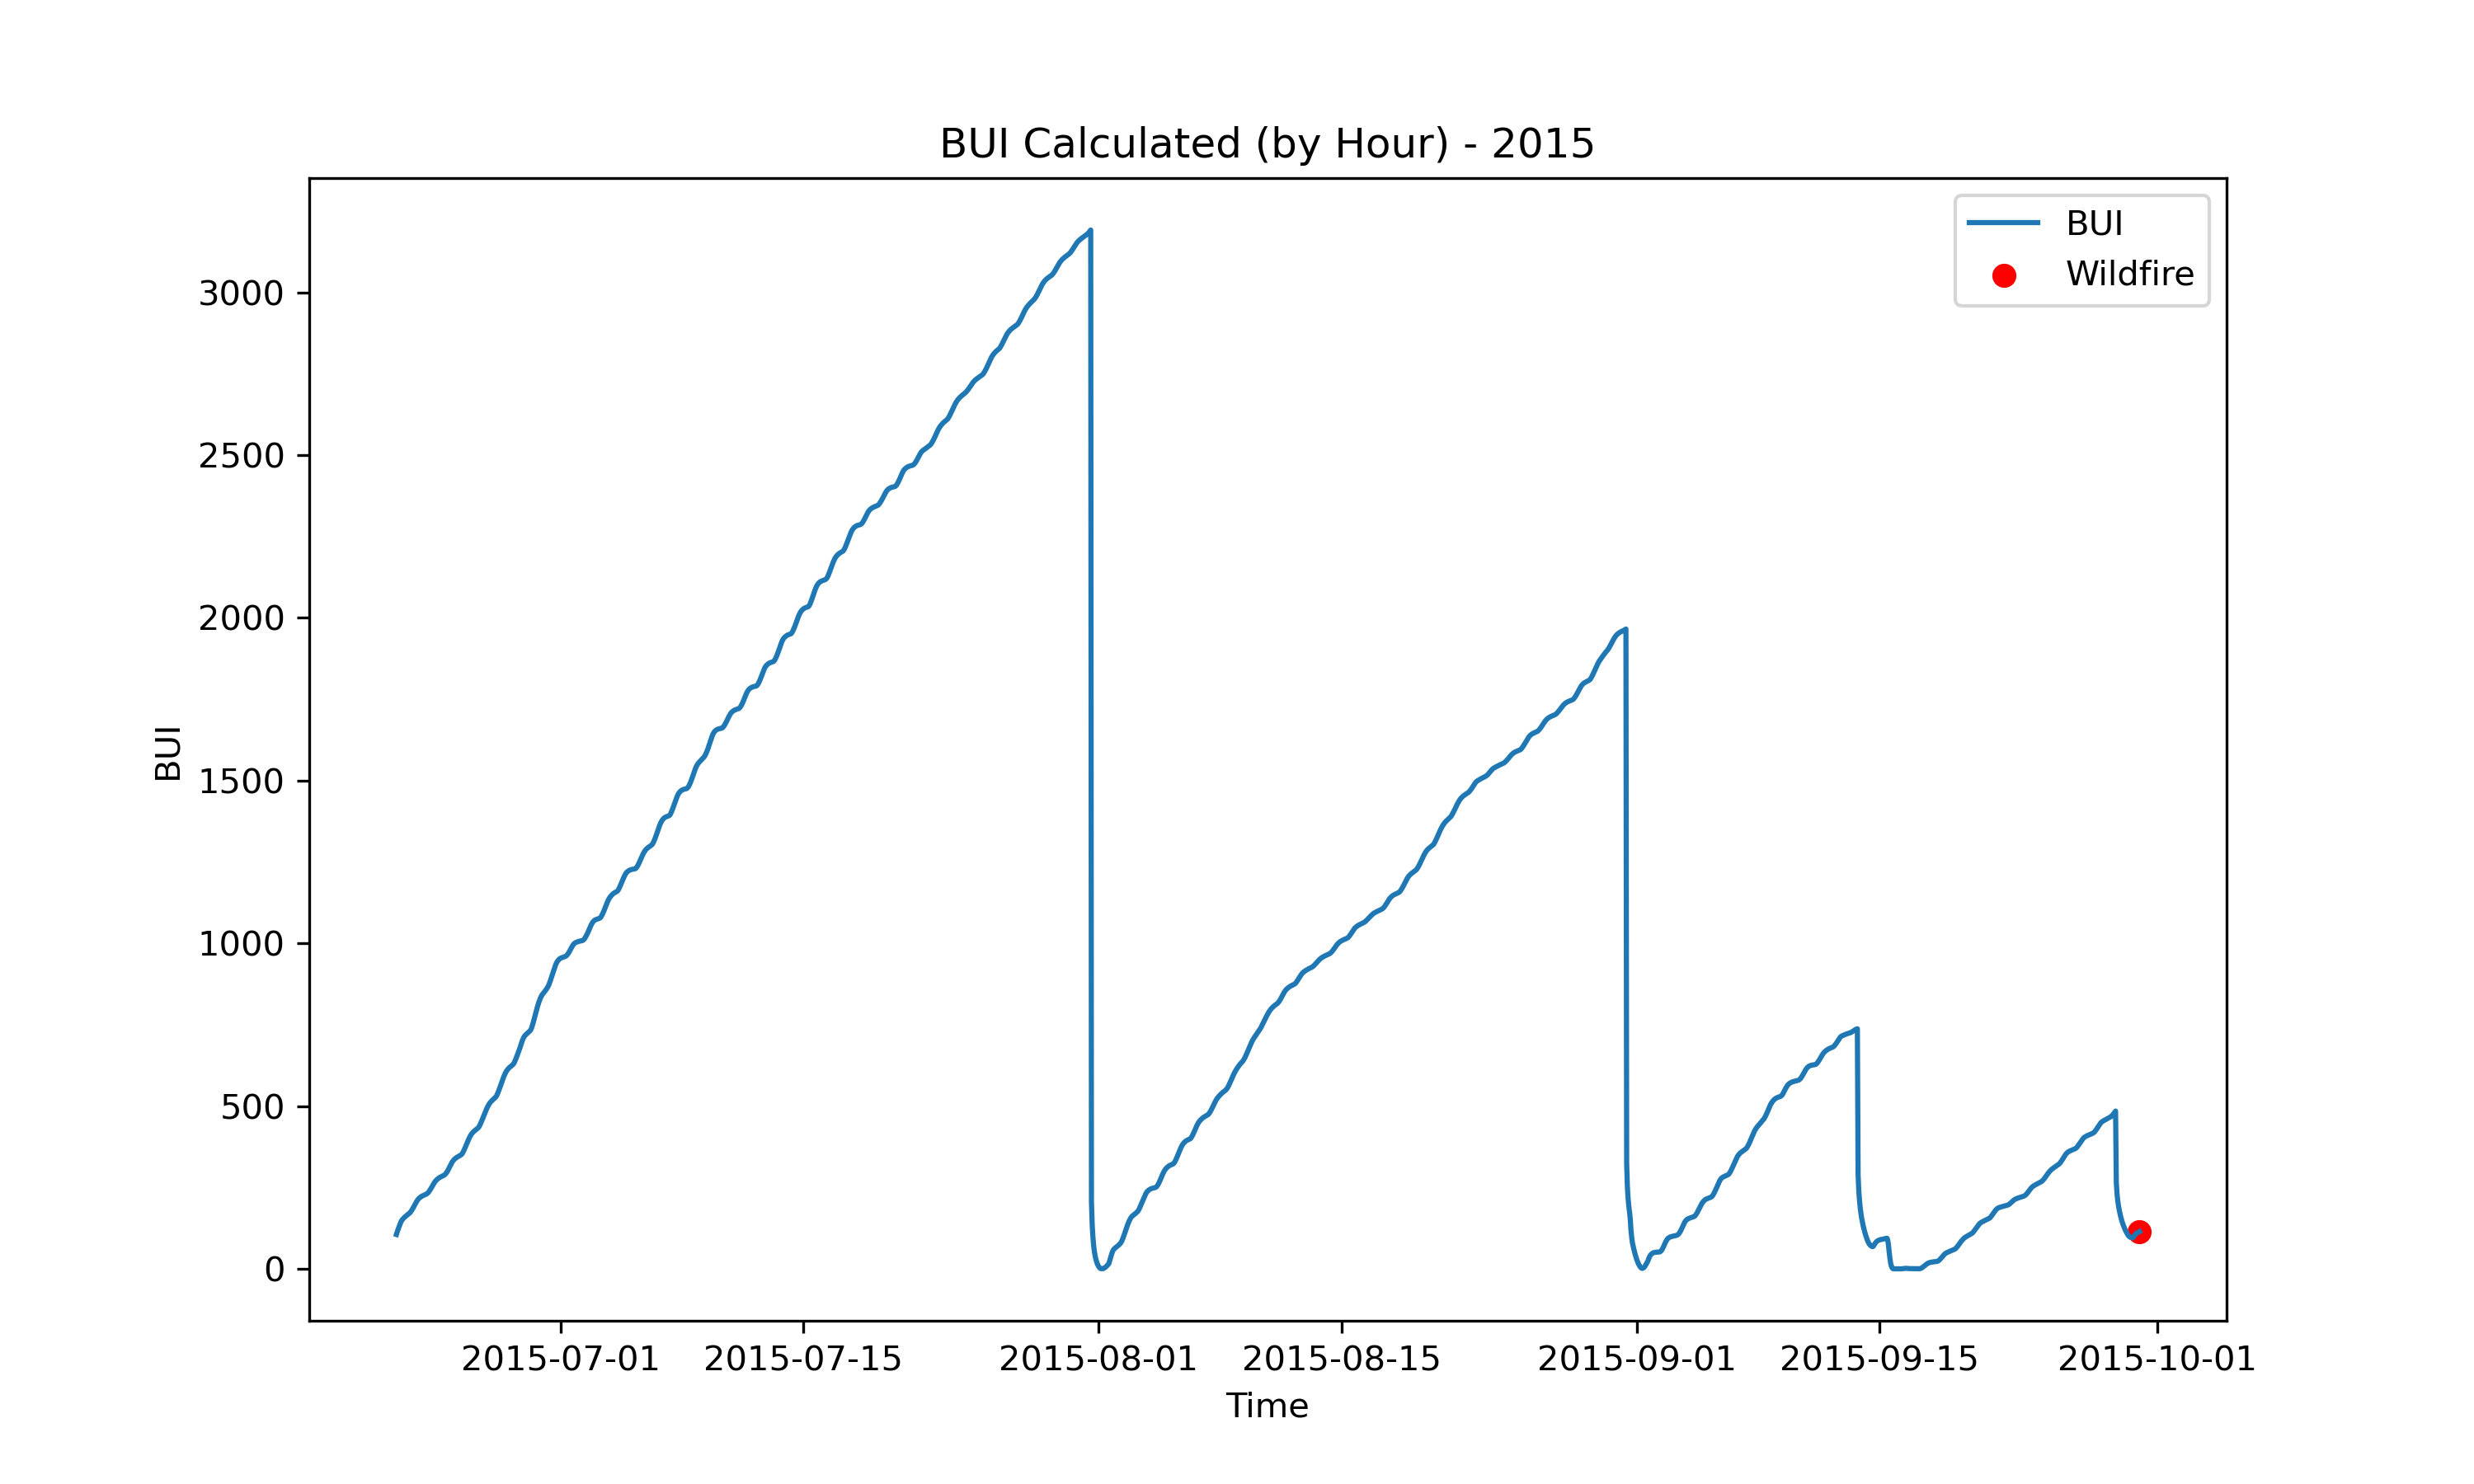
\includegraphics[width=\textwidth]{graphs/2015/byHour/2015CalcBUI12.png}
		\caption{Caption for image 1}
		\label{fig:img1}
	\end{subfigure}
	\hfill
	\begin{subfigure}{0.3\textwidth}
		\centering
		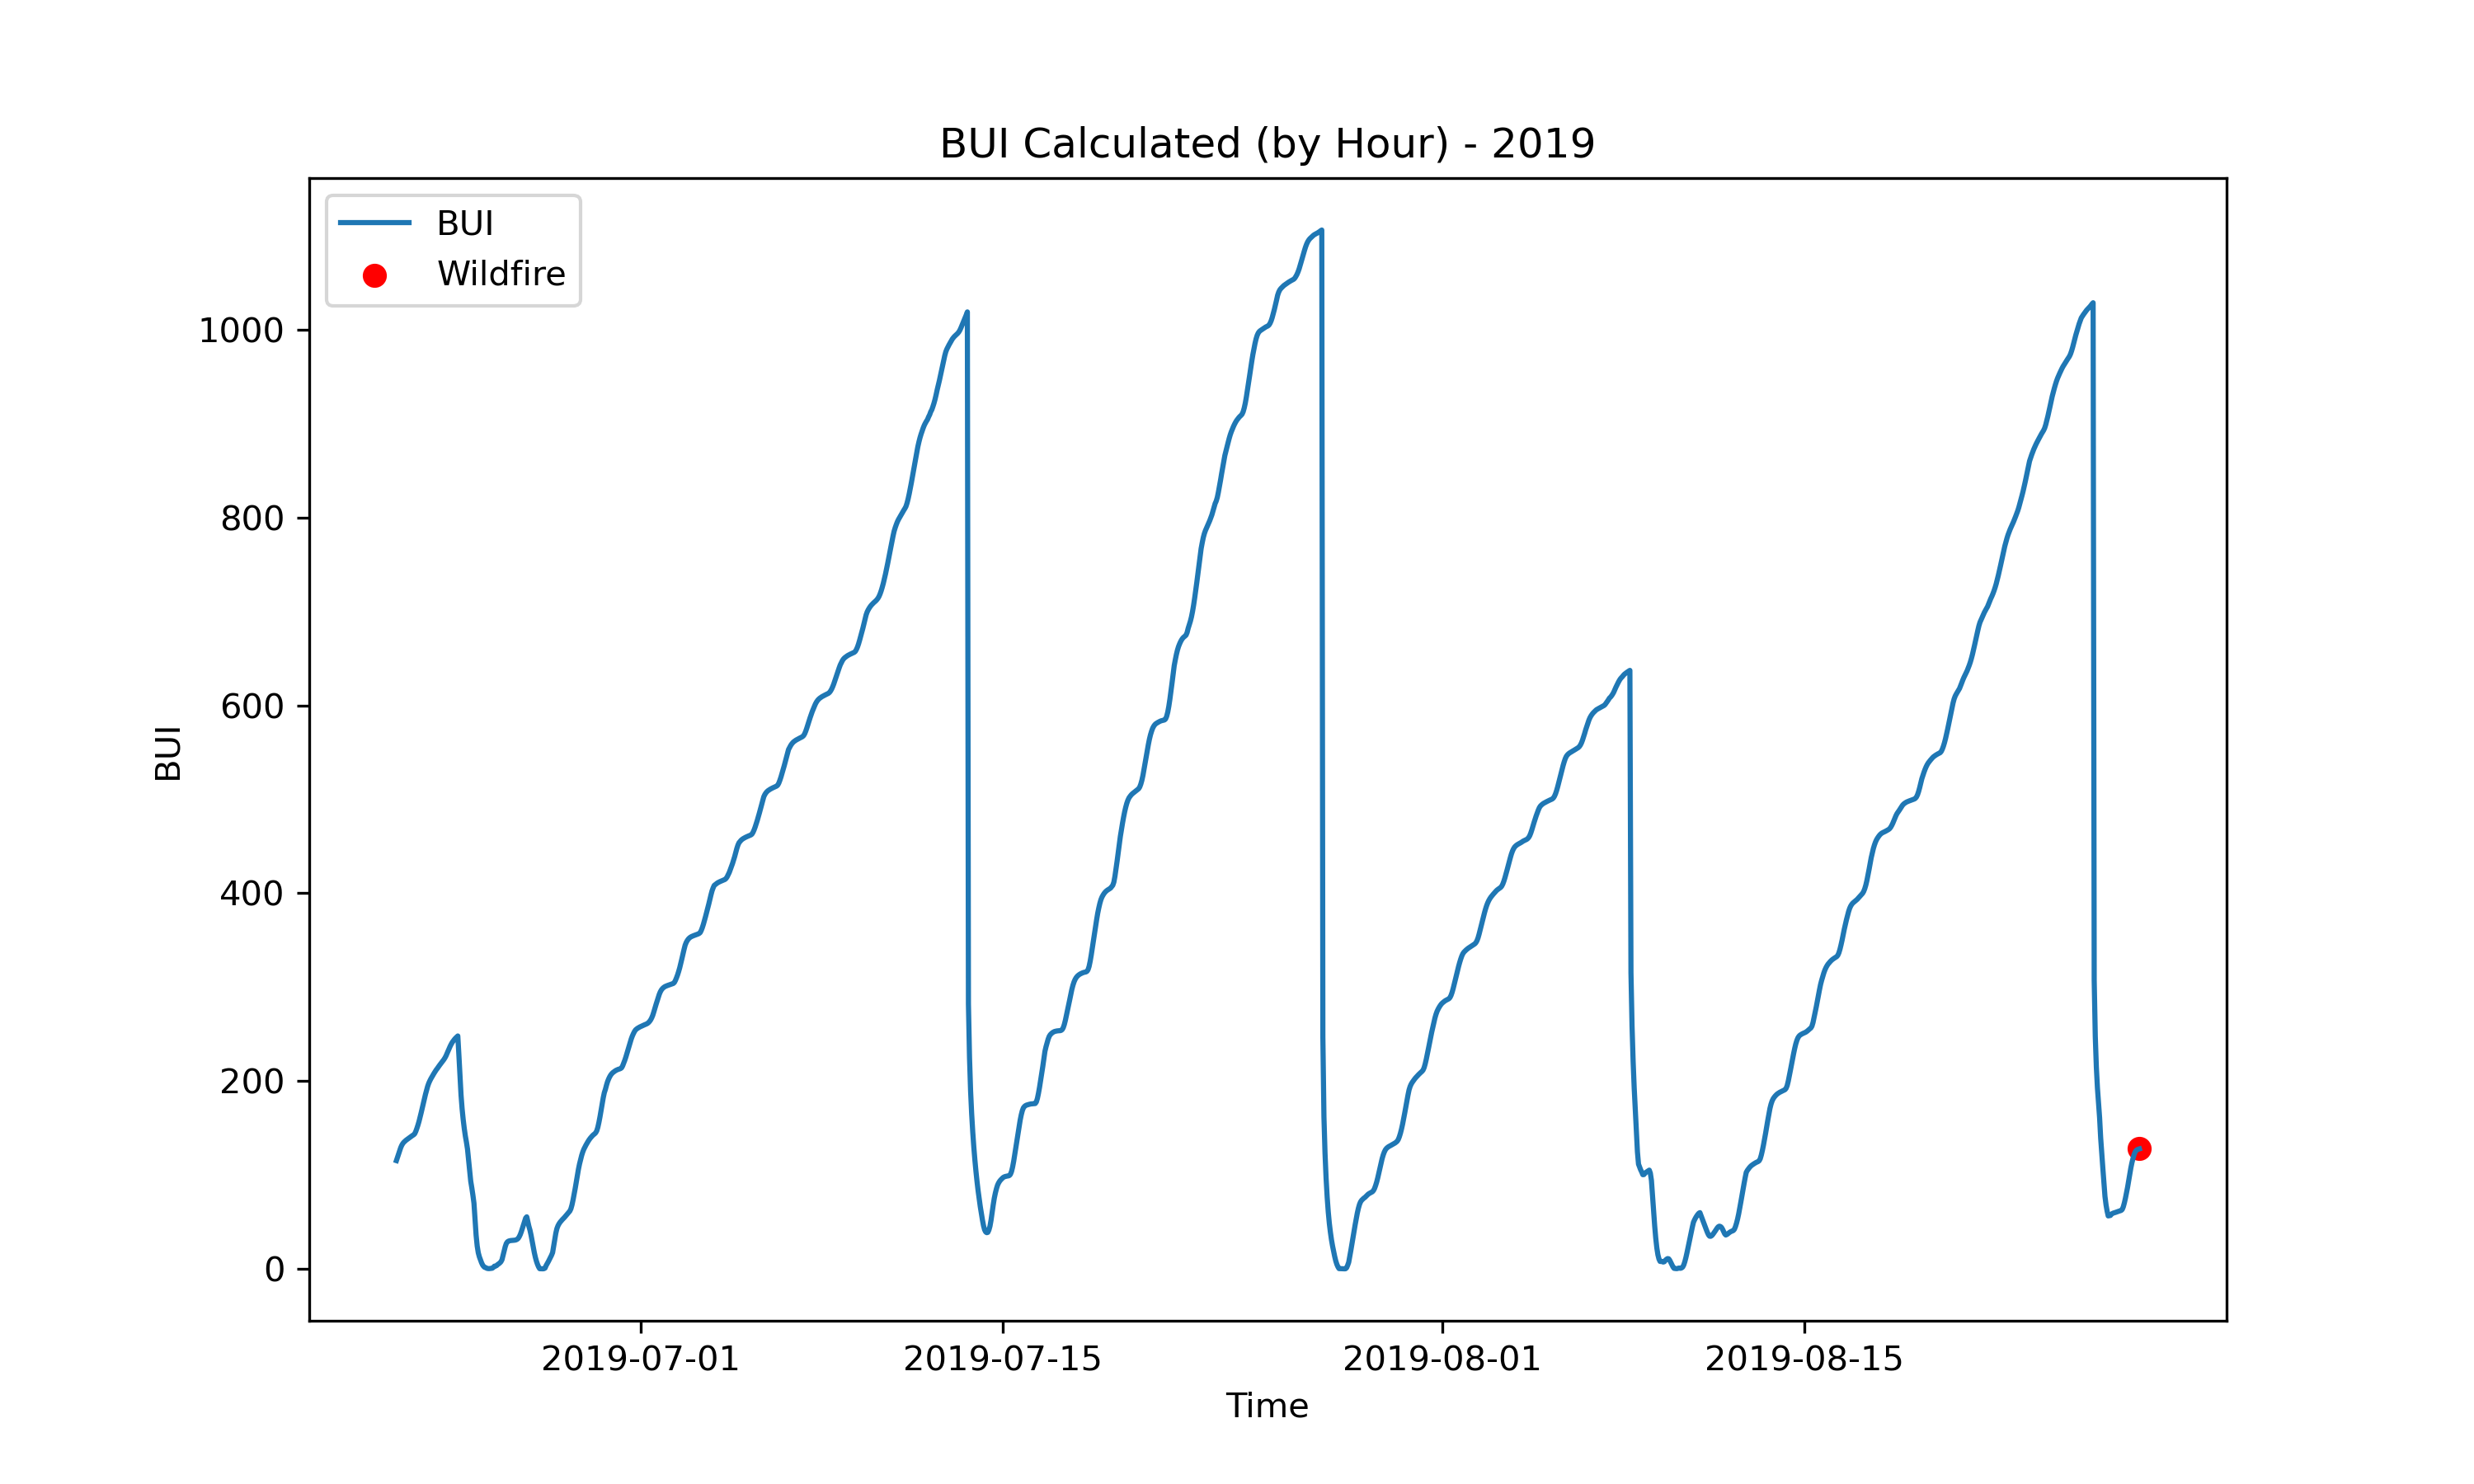
\includegraphics[width=\textwidth]{graphs/2019/byHour/2019CalcBUI12.png}
		\caption{Caption for image 2}
		\label{fig:img2}
	\end{subfigure}
	\hfill
	\begin{subfigure}{0.3\textwidth}
		\centering
		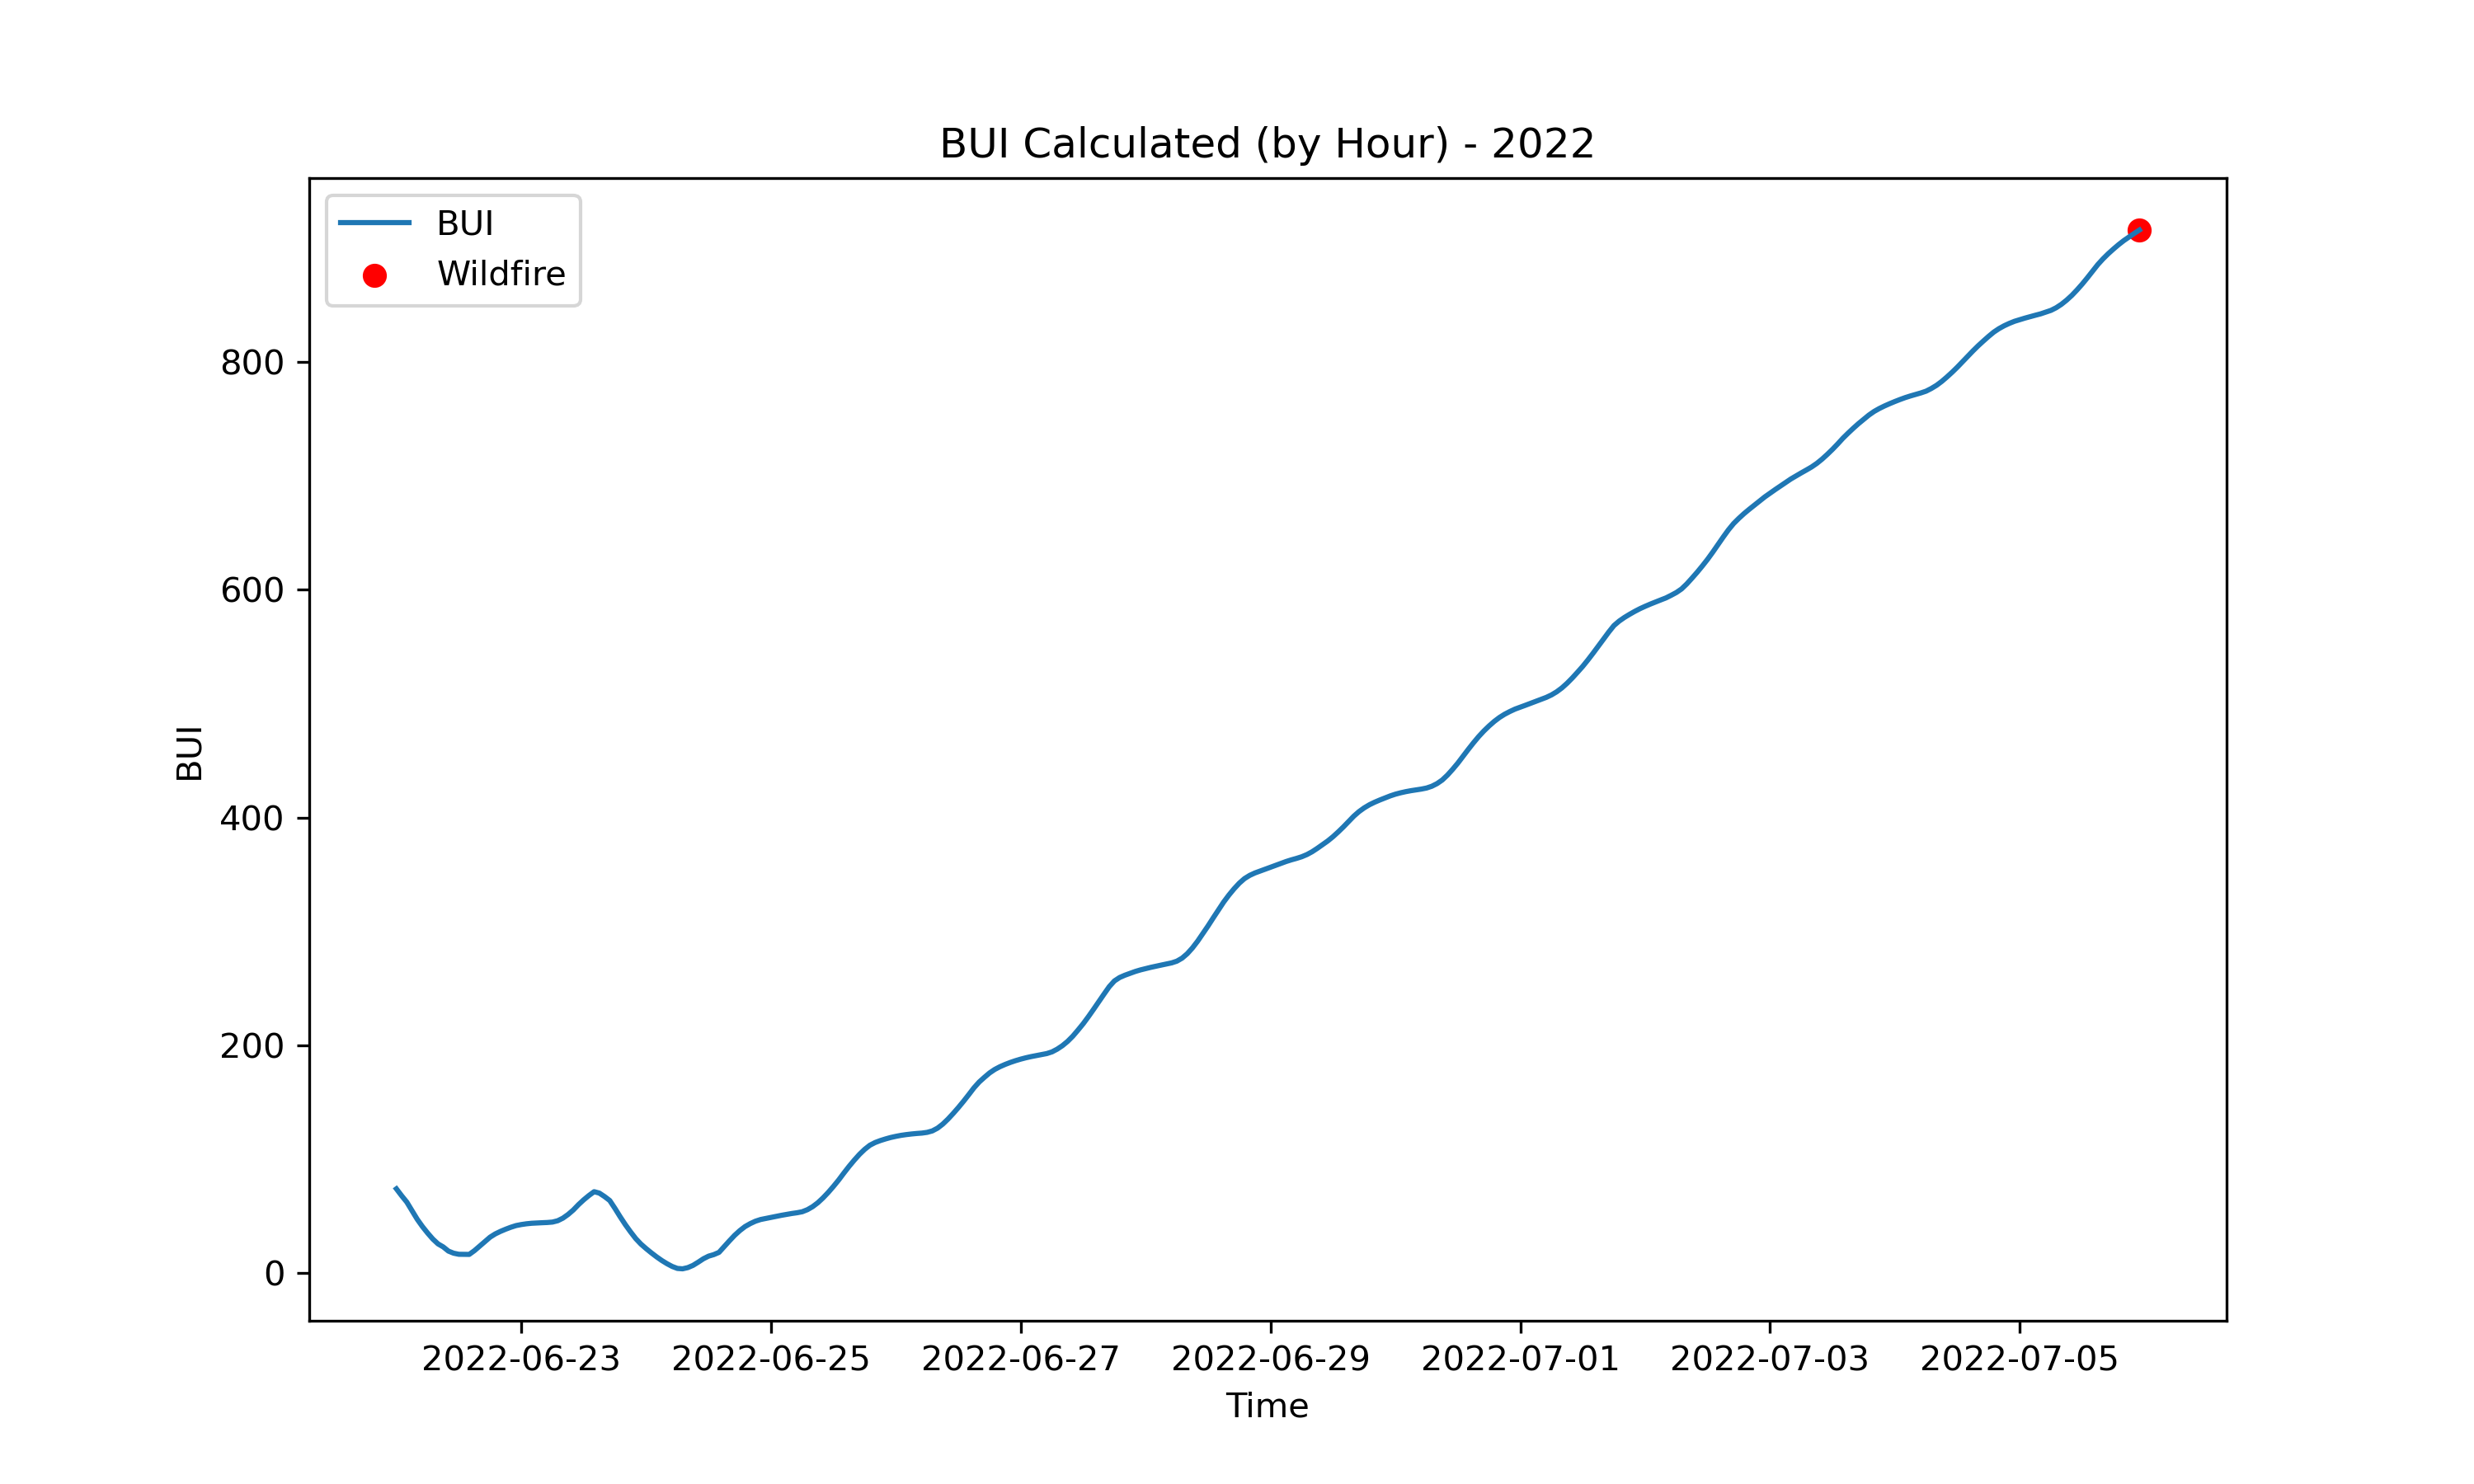
\includegraphics[width=\textwidth]{graphs/2022/2022CalcBUI12.png}
		\caption{Caption for image 3}
		\label{fig:img3}
	\end{subfigure}
	
	\label{fig:all_images}
\end{figure}

\FloatBarrier

\section{Evolution of maximum and minimum daily values of FWI variables}
\begin{figure}[h]
	\centering
	\caption{Caption for the whole figure}
	\begin{subfigure}{0.3\textwidth}
		\centering
		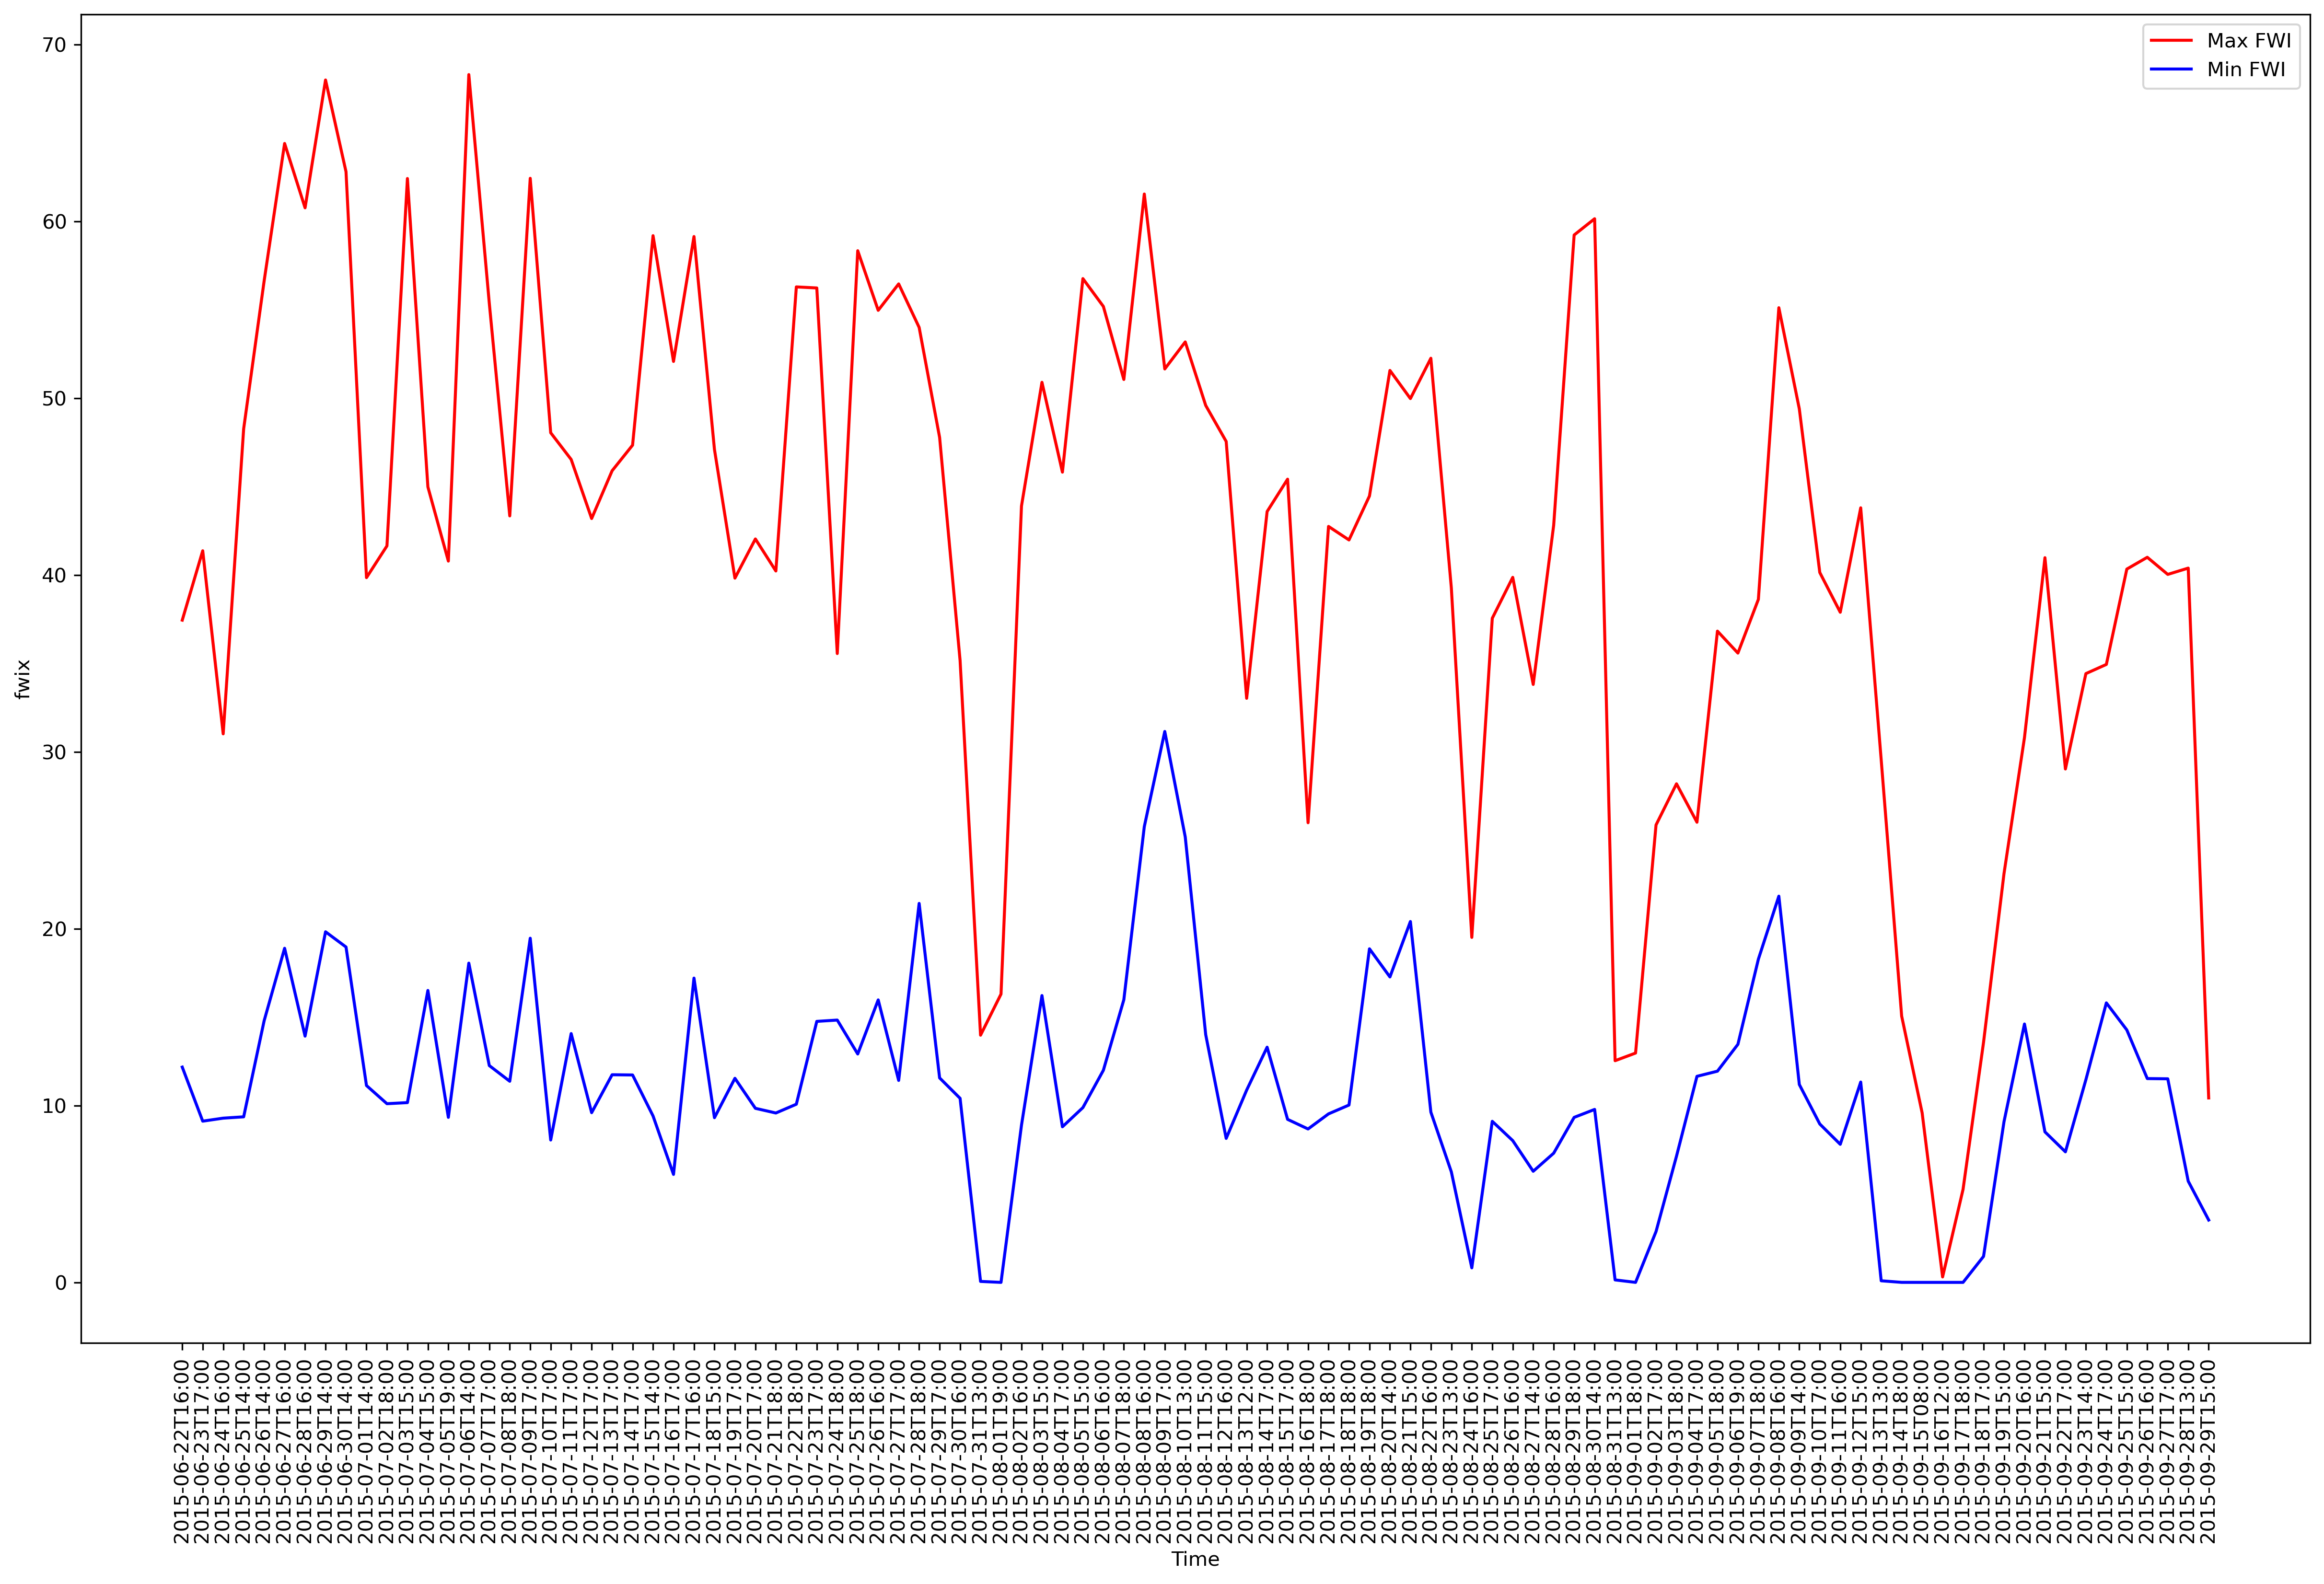
\includegraphics[width=\textwidth]{graphs/2015/byHour/FWI_maxMin.png}
		\caption{Caption for image 1}
		\label{fig:img1}
	\end{subfigure}
	\hfill
	\begin{subfigure}{0.3\textwidth}
		\centering
		\includegraphics[width=\textwidth]{graphs/2019/byHour/FWI_maxMin.png}
		\caption{Caption for image 2}
		\label{fig:img2}
	\end{subfigure}
	\hfill
	\begin{subfigure}{0.3\textwidth}
		\centering
		\includegraphics[width=\textwidth]{graphs/2022/FWI_maxMin.png}
		\caption{Caption for image 3}
		\label{fig:img3}
	\end{subfigure}
	
	\label{fig:all_images}
\end{figure}

\FloatBarrier

\section{Difference between the daily maximum and minimum values of the FWI variables}


\FloatBarrier

\section{3-day time frame mean tendency graphs of FWI variables}
\begin{figure}[h]
	\caption{HELLo}
	\centering
	\begin{subfigure}{0.49\textwidth}
		\centering
		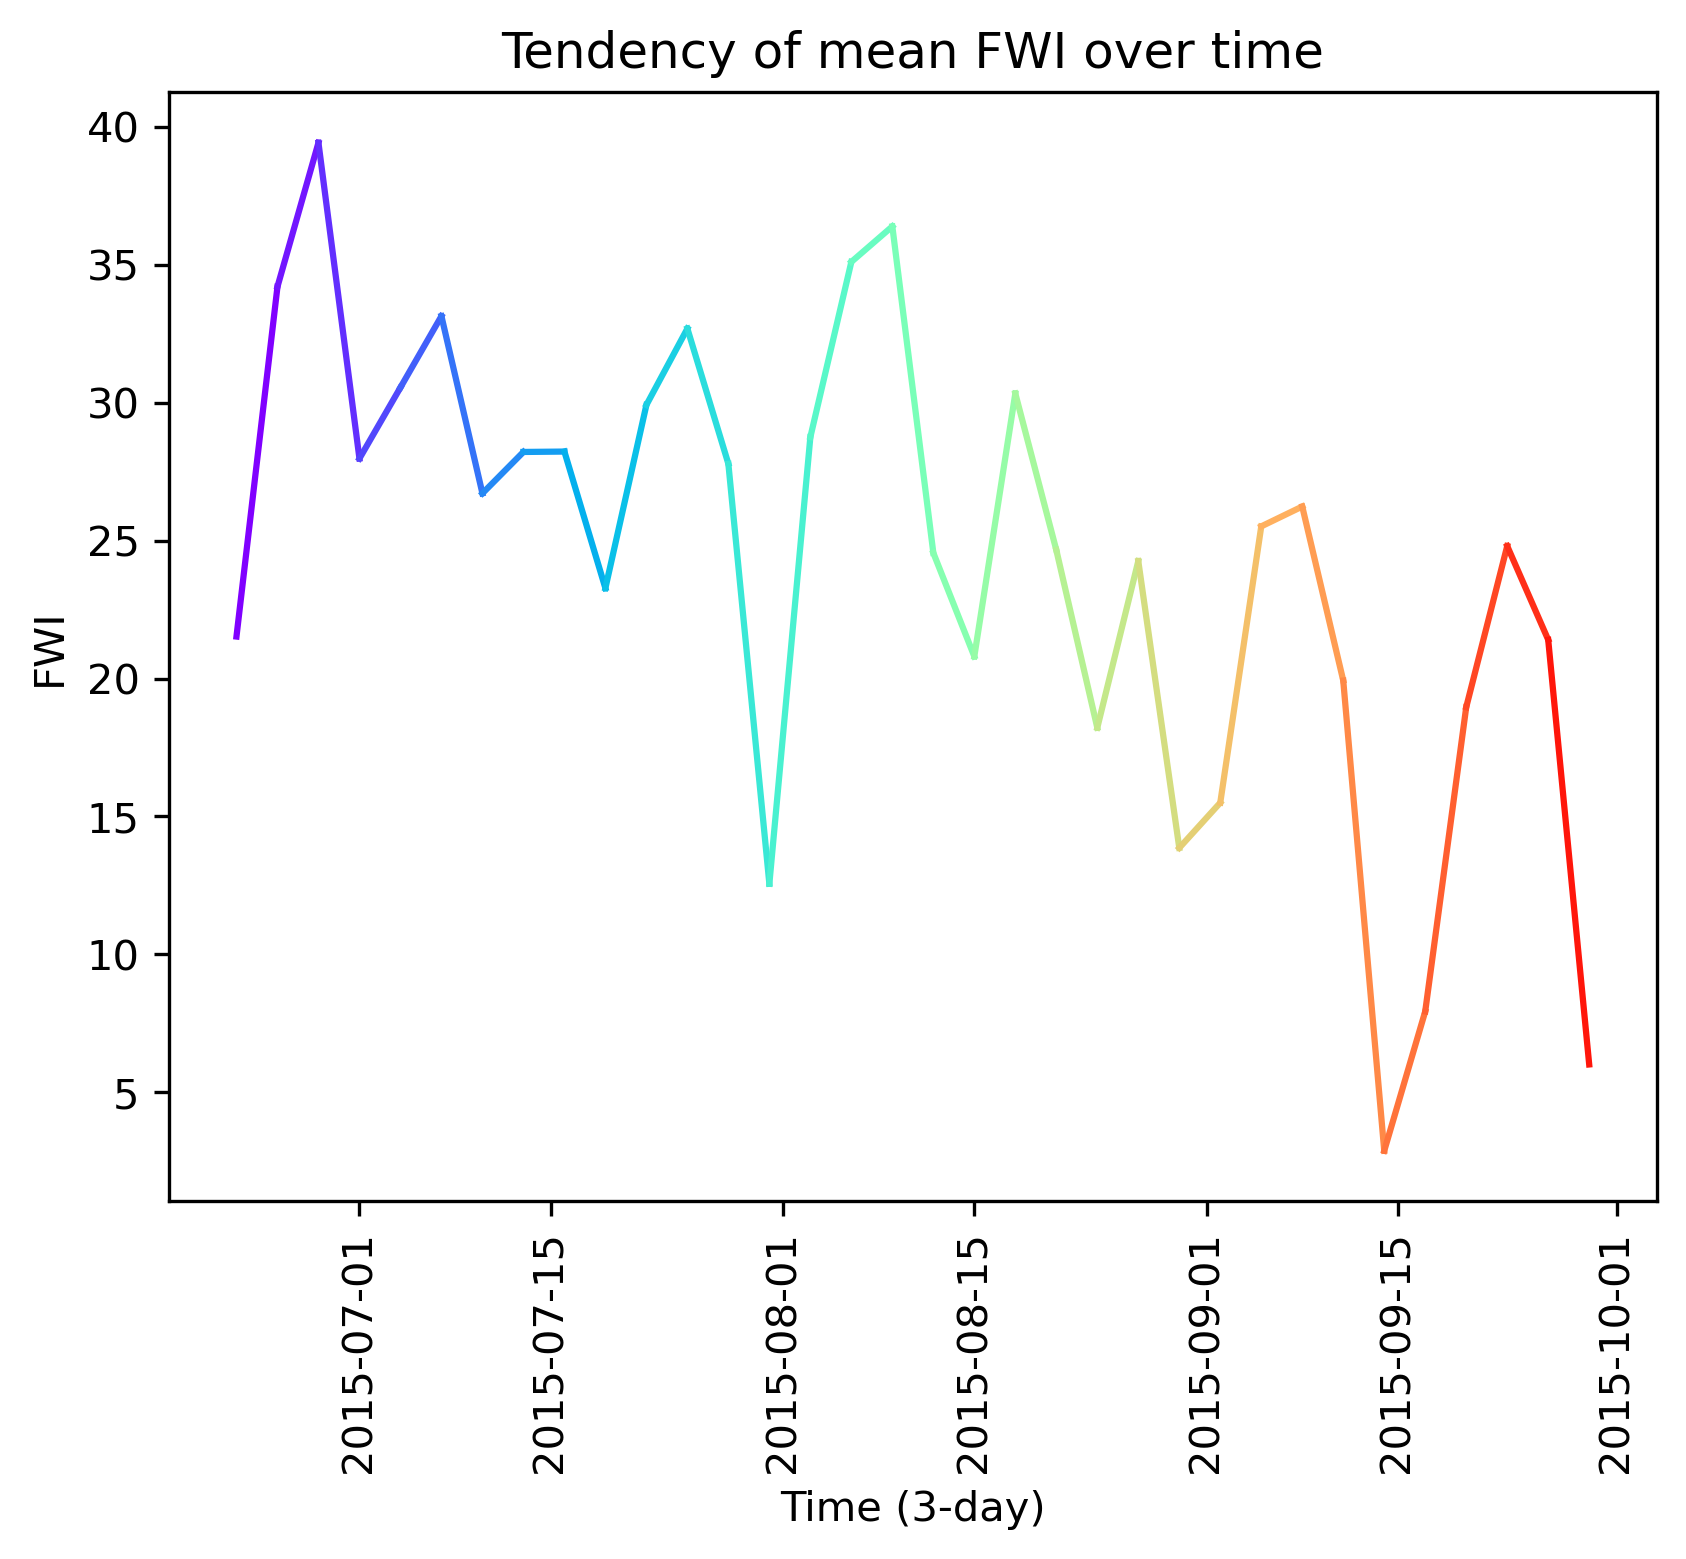
\includegraphics[width=\textwidth]{graphs/2015/tendency/2015_tendency_graph_FWI.png}
		\caption{Caption for image 1}
		\label{fig:img1}
	\end{subfigure}
	\hfill
	\begin{subfigure}{0.49\textwidth}
		\centering
		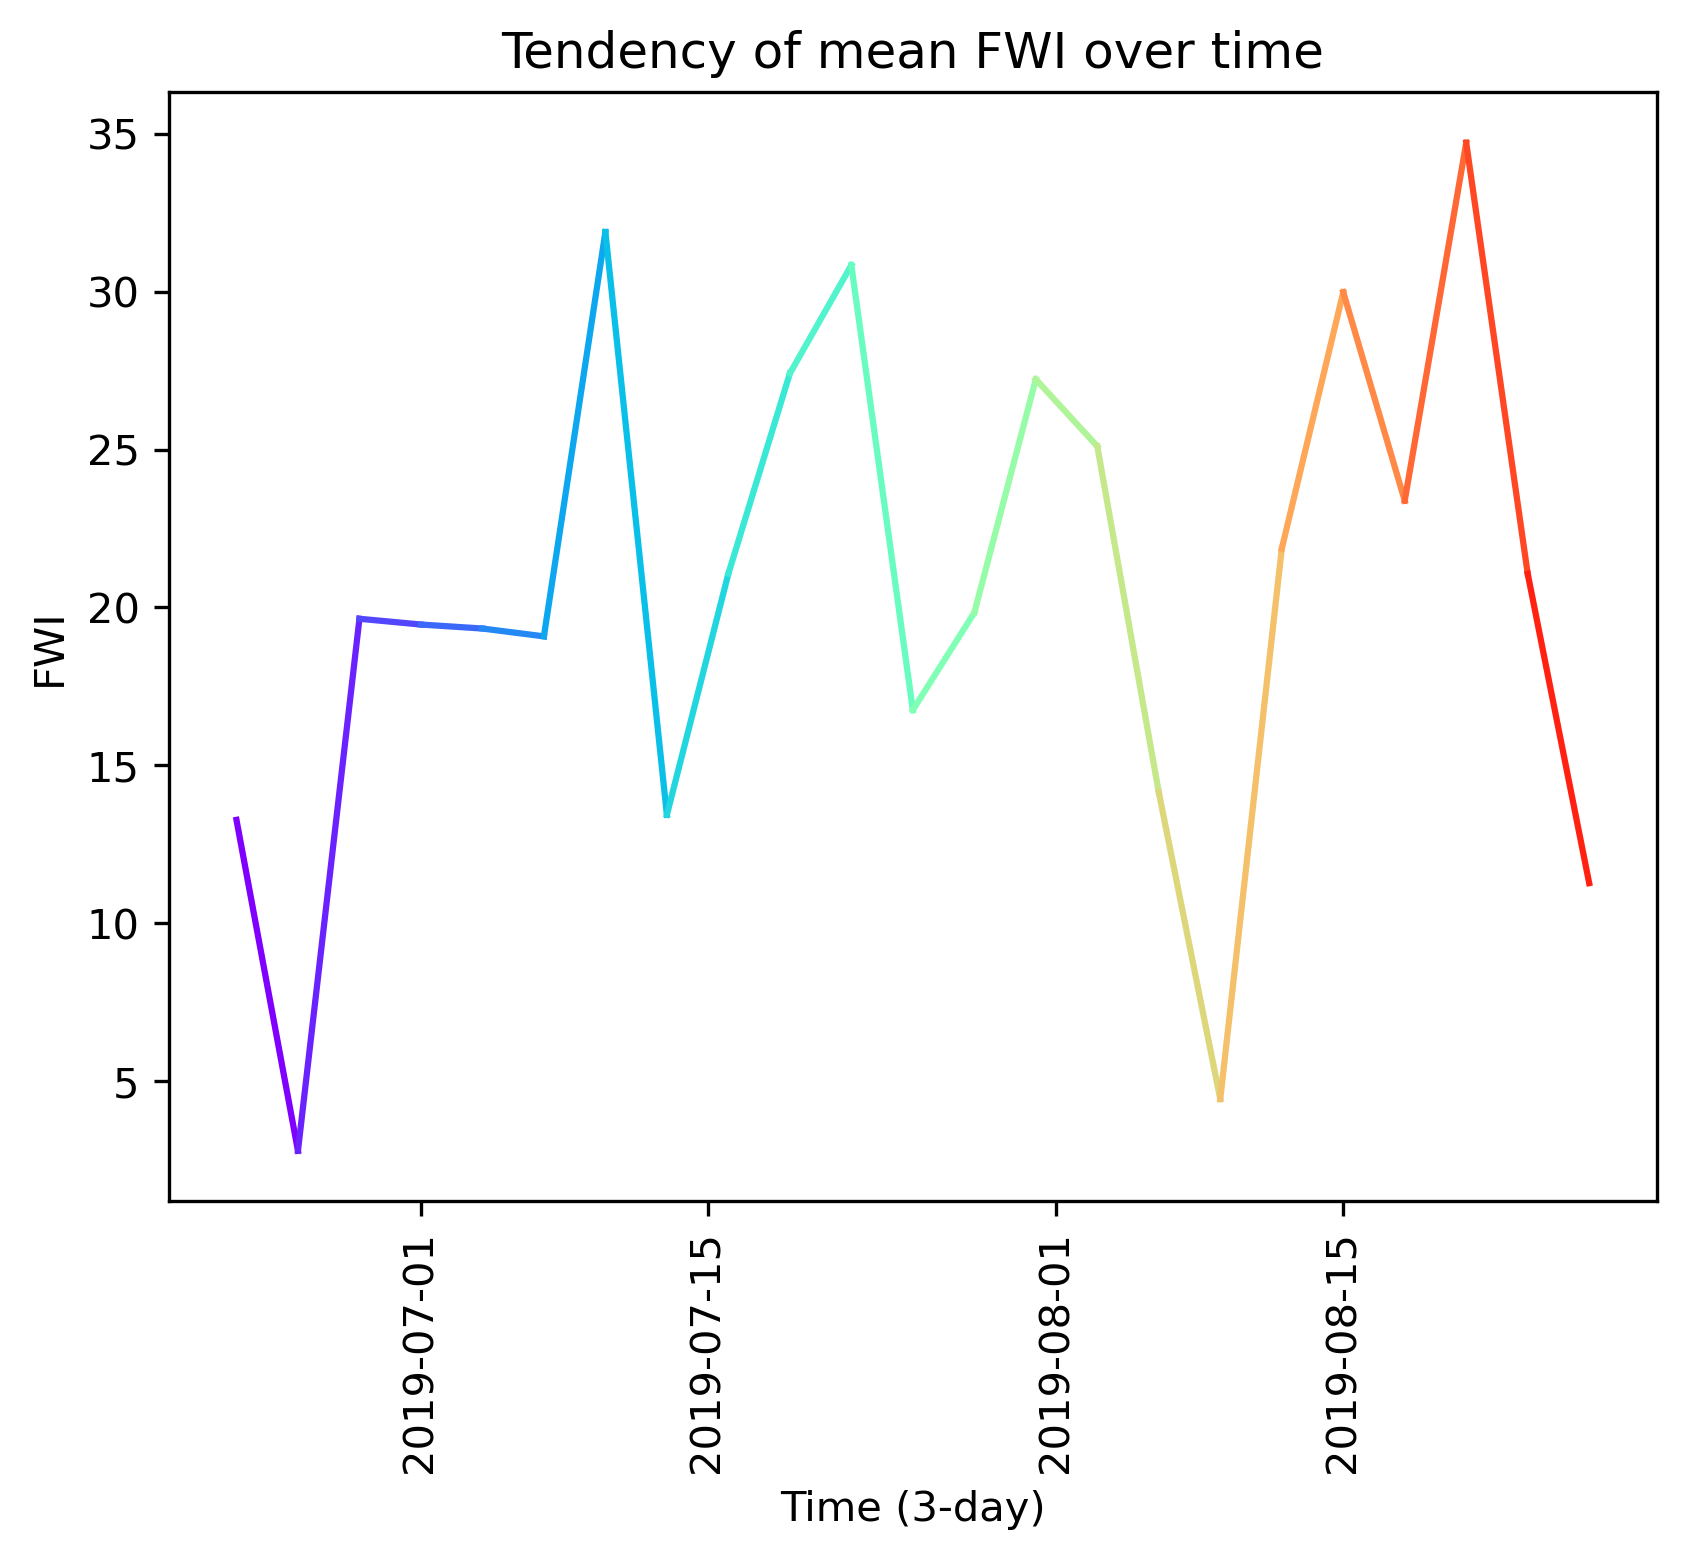
\includegraphics[width=\textwidth]{graphs/2019/tendency/2019_tendency_graph_FWI.png}
		\caption{Caption for image 2}
		\label{fig:img2}
	\end{subfigure}
	\label{fig:both_images}
\end{figure}

\begin{figure}[h]
	\caption{HELLo}
	\centering
	\begin{subfigure}{0.49\textwidth}
		\centering
		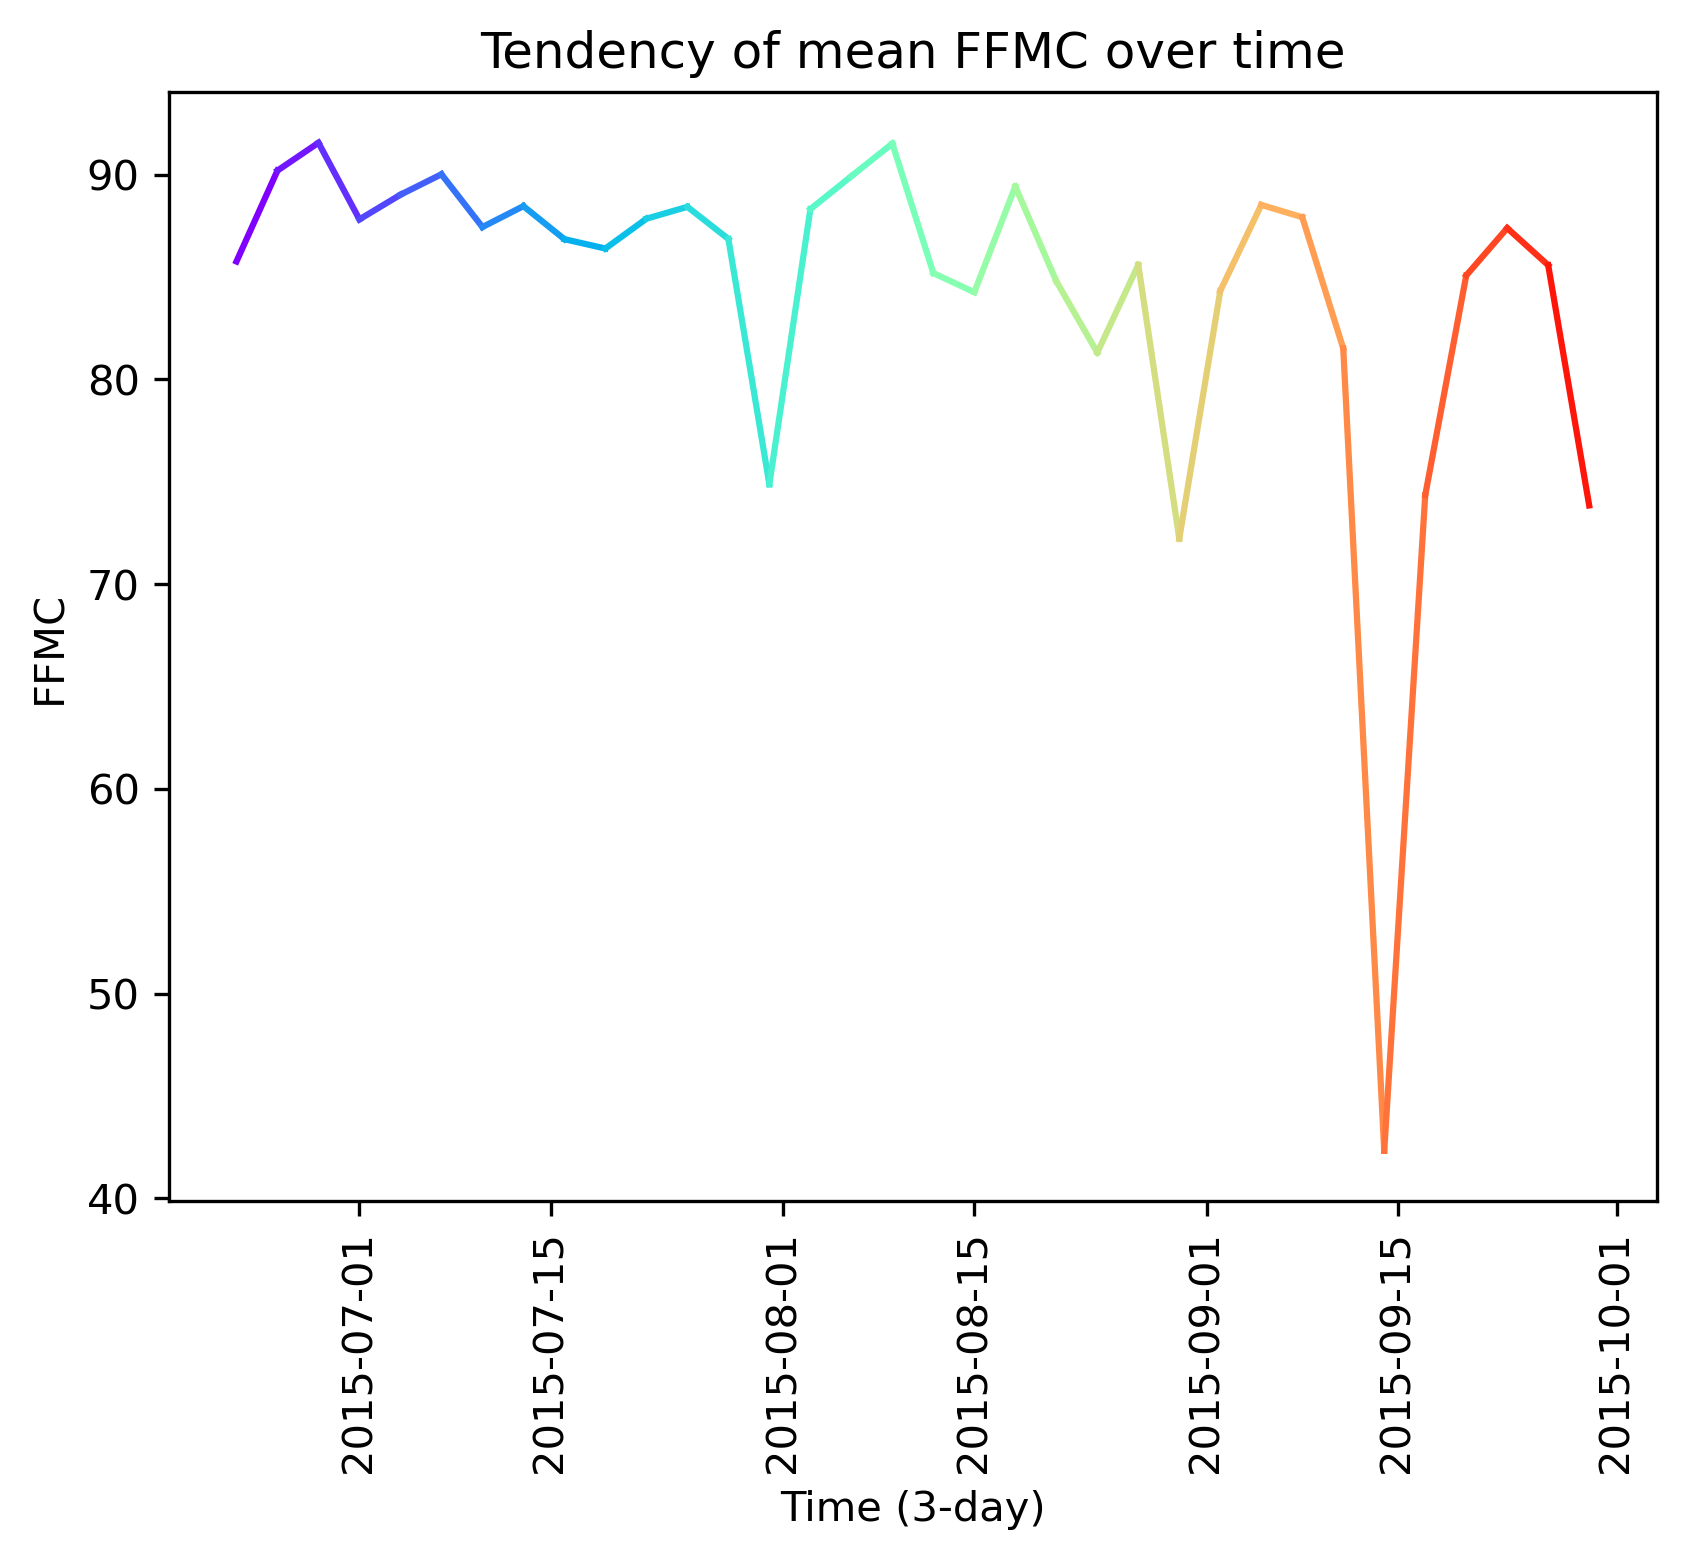
\includegraphics[width=\textwidth]{graphs/2015/tendency/2015_tendency_graph_FFMC.png}
		\caption{Caption for image 1}
		\label{fig:img1}
	\end{subfigure}
	\hfill
	\begin{subfigure}{0.49\textwidth}
		\centering
		\includegraphics[width=\textwidth]{graphs/2019/tendency/2019_tendency_graph_FFMC.png}
		\caption{Caption for image 2}
		\label{fig:img2}
	\end{subfigure}
	\label{fig:both_images}
\end{figure}

\begin{figure}[h]
	\caption{HELLo}
	\centering
	\begin{subfigure}{0.49\textwidth}
		\centering
		\includegraphics[width=\textwidth]{graphs/2015/tendency/2015_tendency_graph_DMC.png}
		\caption{Caption for image 1}
		\label{fig:img1}
	\end{subfigure}
	\hfill
	\begin{subfigure}{0.49\textwidth}
		\centering
		\includegraphics[width=\textwidth]{graphs/2019/tendency/2019_tendency_graph_DMC.png}
		\caption{Caption for image 2}
		\label{fig:img2}
	\end{subfigure}
	\label{fig:both_images}
\end{figure}

\begin{figure}[h]
	\caption{HELLo}
	\centering
	\begin{subfigure}{0.49\textwidth}
		\centering
		\includegraphics[width=\textwidth]{graphs/2015/tendency/2015_tendency_graph_DC.png}
		\caption{Caption for image 1}
		\label{fig:img1}
	\end{subfigure}
	\hfill
	\begin{subfigure}{0.49\textwidth}
		\centering
		\includegraphics[width=\textwidth]{graphs/2019/tendency/2019_tendency_graph_DC.png}
		\caption{Caption for image 2}
		\label{fig:img2}
	\end{subfigure}
	\label{fig:both_images}
\end{figure}

\begin{figure}[h]
	\caption{HELLo}
	\centering
	\begin{subfigure}{0.49\textwidth}
		\centering
		\includegraphics[width=\textwidth]{graphs/2015/tendency/2015_tendency_graph_ISI.png}
		\caption{Caption for image 1}
		\label{fig:img1}
	\end{subfigure}
	\hfill
	\begin{subfigure}{0.49\textwidth}
		\centering
		\includegraphics[width=\textwidth]{graphs/2019/tendency/2019_tendency_graph_ISI.png}
		\caption{Caption for image 2}
		\label{fig:img2}
	\end{subfigure}
	\label{fig:both_images}
\end{figure}

\begin{figure}[h]
	\caption{HELLo}
	\centering
	\begin{subfigure}{0.49\textwidth}
		\centering
		\includegraphics[width=\textwidth]{graphs/2015/tendency/2015_tendency_graph_BUI.png}
		\caption{Caption for image 1}
		\label{fig:img1}
	\end{subfigure}
	\hfill
	\begin{subfigure}{0.49\textwidth}
		\centering
		\includegraphics[width=\textwidth]{graphs/2019/tendency/2019_tendency_graph_BUI.png}
		\caption{Caption for image 2}
		\label{fig:img2}
	\end{subfigure}
	\label{fig:both_images}
\end{figure}




\FloatBarrier

\section{Comparison of mean FWI variables 15 days prior to the wildfire}

\begin{figure}[h]
    \centering
    \caption{Caption for the whole figure}
    \begin{subfigure}{0.3\textwidth}
        \centering
        \includegraphics[width=\textwidth]{graphs/2015/15daysprior/2015_15daysprior_tendency_graph_FWI.png}
        \caption{Caption for image 1}
        \label{fig:img1}
    \end{subfigure}
    \hfill
    \begin{subfigure}{0.3\textwidth}
        \centering
        \includegraphics[width=\textwidth]{graphs/2019/15daysprior/2019_15daysprior_tendency_graph_FWI.png}
        \caption{Caption for image 2}
        \label{fig:img2}
    \end{subfigure}
    \hfill
    \begin{subfigure}{0.3\textwidth}
        \centering
        \includegraphics[width=\textwidth]{graphs/2022/tendency/2022_tendency_graph_FWI.png}
        \caption{Caption for image 3}
        \label{fig:img3}
    \end{subfigure}
    
    \label{fig:all_images}
\end{figure}

\begin{figure}[h]
    \centering
    \caption{Caption for the whole figure}
    \begin{subfigure}{0.3\textwidth}
        \centering
        \includegraphics[width=\textwidth]{graphs/2015/15daysprior/2015_15daysprior_tendency_graph_FFMC.png}
        \caption{Caption for image 1}
        \label{fig:img1}
    \end{subfigure}
    \hfill
    \begin{subfigure}{0.3\textwidth}
        \centering
        \includegraphics[width=\textwidth]{graphs/2019/15daysprior/2019_15daysprior_tendency_graph_FFMC.png}
        \caption{Caption for image 2}
        \label{fig:img2}
    \end{subfigure}
    \hfill
    \begin{subfigure}{0.3\textwidth}
        \centering
        \includegraphics[width=\textwidth]{graphs/2022/tendency/2022_tendency_graph_FFMC.png}
        \caption{Caption for image 3}
        \label{fig:img3}
    \end{subfigure}
    
    \label{fig:all_images}
\end{figure}

\begin{figure}[h]
    \centering
    \caption{Caption for the whole figure}
    \begin{subfigure}{0.3\textwidth}
        \centering
        \includegraphics[width=\textwidth]{graphs/2015/15daysprior/2015_15daysprior_tendency_graph_DMC.png}
        \caption{Caption for image 1}
        \label{fig:img1}
    \end{subfigure}
    \hfill
    \begin{subfigure}{0.3\textwidth}
        \centering
        \includegraphics[width=\textwidth]{graphs/2019/15daysprior/2019_15daysprior_tendency_graph_DMC.png}
        \caption{Caption for image 2}
        \label{fig:img2}
    \end{subfigure}
    \hfill
    \begin{subfigure}{0.3\textwidth}
        \centering
        \includegraphics[width=\textwidth]{graphs/2022/tendency/2022_tendency_graph_DMC.png}
        \caption{Caption for image 3}
        \label{fig:img3}
    \end{subfigure}
    
    \label{fig:all_images}
\end{figure}

\begin{figure}[h]
    \centering
    \caption{Caption for the whole figure}
    \begin{subfigure}{0.3\textwidth}
        \centering
        \includegraphics[width=\textwidth]{graphs/2015/15daysprior/2015_15daysprior_tendency_graph_DC.png}
        \caption{Caption for image 1}
        \label{fig:img1}
    \end{subfigure}
    \hfill
    \begin{subfigure}{0.3\textwidth}
        \centering
        \includegraphics[width=\textwidth]{graphs/2019/15daysprior/2019_15daysprior_tendency_graph_DC.png}
        \caption{Caption for image 2}
        \label{fig:img2}
    \end{subfigure}
    \hfill
    \begin{subfigure}{0.3\textwidth}
        \centering
        \includegraphics[width=\textwidth]{graphs/2022/tendency/2022_tendency_graph_DC.png}
        \caption{Caption for image 3}
        \label{fig:img3}
    \end{subfigure}
    
    \label{fig:all_images}
\end{figure}

\begin{figure}[h]
    \centering
    \caption{Caption for the whole figure}
    \begin{subfigure}{0.3\textwidth}
        \centering
        \includegraphics[width=\textwidth]{graphs/2015/15daysprior/2015_15daysprior_tendency_graph_ISI.png}
        \caption{Caption for image 1}
        \label{fig:img1}
    \end{subfigure}
    \hfill
    \begin{subfigure}{0.3\textwidth}
        \centering
        \includegraphics[width=\textwidth]{graphs/2019/15daysprior/2019_15daysprior_tendency_graph_ISI.png}
        \caption{Caption for image 2}
        \label{fig:img2}
    \end{subfigure}
    \hfill
    \begin{subfigure}{0.3\textwidth}
        \centering
        \includegraphics[width=\textwidth]{graphs/2022/tendency/2022_tendency_graph_ISI.png}
        \caption{Caption for image 3}
        \label{fig:img3}
    \end{subfigure}
    
    \label{fig:all_images}
\end{figure}

\begin{figure}[h]
    \centering
    \caption{Caption for the whole figure}
    \begin{subfigure}{0.3\textwidth}
        \centering
        \includegraphics[width=\textwidth]{graphs/2015/15daysprior/2015_15daysprior_tendency_graph_BUI.png}
        \caption{Caption for image 1}
        \label{fig:img1}
    \end{subfigure}
    \hfill
    \begin{subfigure}{0.3\textwidth}
        \centering
        \includegraphics[width=\textwidth]{graphs/2019/15daysprior/2019_15daysprior_tendency_graph_BUI.png}
        \caption{Caption for image 2}
        \label{fig:img2}
    \end{subfigure}
    \hfill
    \begin{subfigure}{0.3\textwidth}
        \centering
        \includegraphics[width=\textwidth]{graphs/2022/tendency/2022_tendency_graph_BUI.png}
        \caption{Caption for image 3}
        \label{fig:img3}
    \end{subfigure}
    
    \label{fig:all_images}
\end{figure}